% !Mode:: "TeX:UTF-8"

%Composed by Y.B. TANG (ybtang21c@gmail.com), spring-2011
%tex distribution: Texlive / MikTex 2010
%recommended editer: Eclipse + Texlipse
%usage: compile with XeLatex

%option: red, brown, blue
% \documentclass[14pt,mathserif]{beamer}
% \documentclass[14pt]{beamer}
\documentclass[usepdftitle=false, 14pt, handout]{beamer} %无动画
% \documentclass[usepdftitle=false, 14pt]{beamer}

\usepackage{amsmath,amsfonts,amssymb,amsthm,bm}
% \usepackage{txfonts} %another style of math fonts
\usepackage{beamerthemesplit,color,graphics}
\usepackage{ulem} %erase line
\usepackage{esint} %any type of integral symbol
% \usepackage{yhmath} %圆弧帽:\wideparen{AB}

\usepackage{tcolorbox} %各种自定义的盒子
\tcbuselibrary{skins, breakable, theorems}

\usepackage{extarrows}%任意长的等号, \xlongequal

\usepackage{bbding}%各种五角星
% \FiveStar,\FiveStarOpen,\FiveStarLines,\FiveStarShadow
% \FiveStarOutline,\FiveStarCenterOpen,\FiveStarOpenDotted
% \FiveStarConvex,\FiveStarOutlineHeavy,\FiveStarOpenCircled

%==============XeCJK==============================
\usepackage[slantfont,boldfont,CJKchecksingle]{xeCJK}
\setmainfont{Times New Roman}
\setCJKmainfont[BoldFont={Adobe Heiti Std},
	ItalicFont={Adobe Kaiti Std},
    SlantedFont={Adobe Song Std},
%     BoldItalicFont={Weibei SC},
     BoldSlantedFont={Adobe Fangsong Std}
	]{Adobe Heiti Std}
\punctstyle{CCT}
\usepackage{xeCJKfntef}%汉字加点和可断行的下划线

\newCJKfontfamily[Wawa]\Wawati{Wawati SC}
\newCJKfontfamily[STLi]\stliti{STLiti}

%============== Chinese Font Config 2 ===================

% \usepackage{fontspec, xunicode, xltxtra}
% \usepackage{xeCJK}%中文字体
% 
% \setmainfont{Times New Roman}%缺省英文字体 Times New Roman
% \setCJKmainfont[ItalicFont={Adobe Kaiti Std}, 
% 	BoldFont={Adobe Heiti Std}]{Adobe Song Std}%衬线字体 缺省中文字体
% \setCJKsansfont{Adobe Heiti Std}%serif是有衬线字体sans serif无衬线字体。
% \setCJKmonofont{Adobe Fangsong Std}%中文等宽字体

%======== customer defined fonts and fontsize ============

% %-----------------------xeCJK下设置中文字体------------------------------%
%常用字体
\setCJKfamilyfont{song}{Adobe Song Std}				%Adobe宋 \song
\newcommand{\song}{\CJKfamily{song}}                
      
\setCJKfamilyfont{fsong}{Adobe Fangsong Std}			%adobe仿宋 \fsong
\newcommand{\fsong}{\CJKfamily{fsong}}

\setCJKfamilyfont{kai}{Adobe Kaiti Std}				%Adobe楷体 \kaiti
\newcommand{\kaiti}{\CJKfamily{kai}}

\setCJKfamilyfont{hei}{Adobe Heiti Std}				%Adobe黑体 \heiti
\renewcommand{\heiti}{\CJKfamily{hei}}

\setCJKfamilyfont{hwzs}{STZhongsong}				%华文中宋 \hwzs
\newcommand{\hwzs}{\CJKfamily{hwzs}}

\setCJKfamilyfont{yh}{Microsoft YaHei}				%微软雅黑 \msyh
\newcommand{\msyh}{\CJKfamily{yh}}

%其他字体
\setCJKfamilyfont{hwfs}{STFangsong}				%华文仿宋  hwfs
\newcommand{\hwfs}{\CJKfamily{hwfs}}

\setCJKfamilyfont{hwxh}{STXihei}					%华文细黑  hwxh
\newcommand{\hwxh}{\CJKfamily{hwxh}}

\setCJKfamilyfont{hwl}{STLiti}						%华文隶书  hwl
\newcommand{\hwls}{\CJKfamily{hwl}}

\setCJKfamilyfont{hwxw}{STXinwei}					%华文新魏  hwxw
\newcommand{\hwxw}{\CJKfamily{hwxw}}

\setCJKfamilyfont{hwxk}{STXingkai}					%华文行楷  hwxk
\newcommand{\hwxk}{\CJKfamily{hwxk}}

\setCJKfamilyfont{hwhp}{STHupo}					%华文琥珀   hwhp
\newcommand{\hwhp}{\CJKfamily{hwhp}}

\setCJKfamilyfont{wawati}{Wawati SC}				%娃娃体 wawati
\newcommand{\wawati}{\CJKfamily{wawati}}

%------------------------------设置字体大小------------------------%
\newcommand{\chuhao}{\fontsize{42pt}{\baselineskip}\selectfont}     %初号
\newcommand{\xiaochuhao}{\fontsize{36pt}{\baselineskip}\selectfont} %小初号
\newcommand{\yihao}{\fontsize{28pt}{\baselineskip}\selectfont}      %一号
\newcommand{\erhao}{\fontsize{21pt}{\baselineskip}\selectfont}      %二号
\newcommand{\xiaoerhao}{\fontsize{18pt}{\baselineskip}\selectfont}  %小二号
\newcommand{\sanhao}{\fontsize{15.75pt}{\baselineskip}\selectfont}  %三号
\newcommand{\sihao}{\fontsize{14pt}{\baselineskip}\selectfont}%     四号
\newcommand{\xiaosihao}{\fontsize{12pt}{\baselineskip}\selectfont}  %小四号
\newcommand{\wuhao}{\fontsize{10.5pt}{\baselineskip}\selectfont}    %五号
\newcommand{\xiaowuhao}{\fontsize{9pt}{\baselineskip}\selectfont}   %小五号
\newcommand{\liuhao}{\fontsize{7.875pt}{\baselineskip}\selectfont}  %六号
\newcommand{\qihao}{\fontsize{5.25pt}{\baselineskip}\selectfont}    %七号

\usefonttheme{professionalfonts}

\newcommand{\fs}[1]{\fontspec{#1}\CJKfontspec{#1}}

%

% %==============std fontspec settings==============
% \usepackage[no-math,cm-default]{fontspec}
% % \newfontfamily\zhfont[BoldFont=Adobe Heiti Std]{Adobe Heiti Std}
% \newfontfamily\zhfont[BoldFont=Adobe Heiti Std]{Adobe Kaiti Std}
% % 
% % %==============spacing of CH in Xetex==============
% \usepackage{zhspacing}
% \zhspacing

%==============layout setting==============
\setlength{\parindent}{0pt}  

%==============beamer configuration==============
\setbeamertemplate{theorems}[normal font]

%============beamer theme setting #2============
\mode<presentation>{
	\usetheme{CambridgeUS} %Copenhagen, Warsaw, CambridgeUS
  	\usecolortheme{rose} %rose, seahorse, lily, crane
  	\usefonttheme{serif}
  	\usefonttheme{structurebold}
  	\useoutertheme{infolines}
%   \beamertemplateshadingbackground{brown!5}{yellow!10}
% 	\setbeamercolor{frametitle}{bg=white}	
%  	\setbeamercovered{transparent}
}

%============TOC setting============
% \AtBeginSection{
%    \begin{frame}{内容提要}
%      \tableofcontents[currentsection,hideallsubsections]
%    \end{frame}
% }
% \AtBeginSubsection{
%    \begin{frame}{内容提要}
%      \tableofcontents[currentsection,currentsubsection]
%    \end{frame}
% }
% \AtBeginSection{
%   \frame{\tableofcontents[sections={\thesection}]}
% }

%===============macros====================
% \newcommand{\bb}{\bf\color{blue}}
% \newcommand{\ba}[1]{\alert{\bf #1}}
% \newcommand*{\e}{\ensuremath{\varepsilon}}
% \renewcommand{\b}{\color{blue}}
% \newcommand*{\p}{\ensuremath{\partial}}
% \newcommand{\limn}{\ensuremath{\lim\limits_{n\to\infty}}}
% \newcommand{\sumn}{\ensuremath{\sum\limits_{n=1}^{\infty}}}
% \newcommand*{\df}[2]{\displaystyle\frac{\,{#1}\,}{\,{#2}\,}}
% \newcommand*{\limx}[1]{\ensuremath{\lim\limits_{x\to{#1}}}}
% \newcommand*{\limdx}{\ensuremath{\lim\limits_{\Delta x\to 0}}}
% \newcommand*{\dx}{\Delta x}
% \newcommand{\dint}{\ensuremath{\displaystyle\int}}
% \renewcommand{\d}{\mathrm{d}}
% \newcommand{\ds}{\displaystyle}

%===============macros====================
\def\ds{\displaystyle}
\def\fin{\hfill$\Box$}
\def\bs{\bigskip}
\def\b{\color{blue!80!yellow}}
\def\bb{\bf\color{blue}}
\def\e{\ensuremath{\varepsilon}}

\newcommand{\ba}[1]{\alert{\bf #1}}
\providecommand{\mbb}[1]{\ensuremath{\mathbb{{#1}}}}
\providecommand{\mr}[1]{\ensuremath{\mathrm{{#1}}}}


\newcommand{\limn}{\ensuremath{\lim\limits_{n\to\infty}}}
\newcommand*{\limx}[1]{\ensuremath{\lim\limits_{x\to{#1}}}}
\newcommand*{\limdx}{\ensuremath{\lim\limits_{\Delta x\to 0}}}
\providecommand{\llim}[1]{\ensuremath{\lim\limits_{#1}}}

\newcommand{\sumn}{\ensuremath{\sum\limits_{n=1}^{\infty}}}
\providecommand{\sumk}[1]{\ensuremath{\sum\limits_{k={#1}}^n}}
\providecommand{\suml}{\ensuremath{\sum\limits}}

\newcommand*{\df}[2]{\displaystyle\frac{\,{#1}\,}{\,{#2}\,}}
\newcommand*{\dx}{\Delta x}
\renewcommand{\d}{\mathrm{d}}
\newcommand*{\p}{\ensuremath{\partial}}

\newcommand{\dint}{\ensuremath{\displaystyle\int}}

\newcommand{\ps}[1]{$^{[\mbox{\it\footnotesize 注}]}$
\marginpar{\kaiti\small {注:}#1}}

%define tab of .25 textwidth and can auto strech
%\tab{the word}\tab{another word}\tab{3rd one}
\newlength{\tabcont}
\newcommand{\tab}[1]{%
	\settowidth{\tabcont}{#1}%
	\ifthenelse{\lengthtest{\tabcont < .25\linewidth}}%
	{\makebox[.25\linewidth][l]{#1}\ignorespaces}%
	%{\makebox[.5\linewidth][l]{\color{red} #1}\ignorespaces}%
	{\makebox[.5\linewidth][l]{#1}\ignorespaces}%
}%

%set fontsize with number of points
% \newcommand{\fs}[1]{\fontsize{#1 pt}{5pt}\selectfont}

\newtcolorbox{thx}{colframe=blue!40!black,colback=white,breakable}

\newtcolorbox{ext}{colframe=green!60!black,colback=green!20!white,breakable}



%================exampleblock counter===================
% \newcounter{examplecounter}
% \usecounter{examplecounter}
% \setcounter{examplecounter}{1}
% \newcommand{\exno}{{\bf
% 例\arabic{examplecounter}}\refstepcounter{examplecounter}}

%================block setting test=====================
% \definecolor{beamer@blendedred}{rgb}{0.7,0.2,0.2} % use structure theme to change
% \definecolor{beamer@blendedblue}{rgb}{0.2,0.2,0.7} % use structure theme to change
% \definecolor{beamer@blendedyellow}{rgb}{0.7,0.7,0.2}

% \setbeamercolor{structure}{fg=beamer@blendedred}

% \setbeamercolor{block title}
% {use=structure,fg=structure.fg,bg=structure.fg!20!bg}
% \setbeamercolor{block title alerted}
% {use=alerted text,fg=alerted text.fg,bg=alerted text.fg!20!bg}
% \setbeamercolor{block title example}
% {use=example text,fg=example text.fg,bg=example text.fg!20!bg}

% \setbeamercolor{block body}
% {parent=normal text,use=block title,bg=block title.bg!50!bg}
% \setbeamercolor{block body alerted}
% {parent=normal text,use=block title alerted,bg=block title alerted.bg!50!bg}
% \setbeamercolor{block body example}
% {parent=normal text,use=block title example,bg=block title example.bg!50!bg}

% \setbeamercolor{titlelike}{parent=structure,bg=white!90!red}
%=======================================================

%===============title setting====================

% \title{Advanced Mathematics II}
% \author[ybtang@nudt.edu.cn]{唐扬斌\\
% \texttt{\small ybtang21c@gmail.com\\tangyangbin@gfkd.mtn\\CP: 18374857376}}
% \institute[NUDT]{National University of Defense Technology}
% \date[Spring 2017]{Spring 2017}

% \title{作业讲评}
\title{作业讲评}
% \title{常微分方程小结与补充例题}
% \title{随堂测验}

%===============document begins here==============

\begin{document}

% % !Mode:: "TeX:UTF-8"

\titlepage

\begin{frame}{说在前面}
	\linespread{1.5}
	  \begin{itemize}[<+-|alert@+>]
	    \item 作业中打$\color{red}\times$的必须订正,否则下次不予批改,
		默认评分为$C$以下;
	    \item 写过的作业不许撕掉,除非重写;
	    \item 不要忘记贴照片,作业本封面注明学员队和班号;
	    \item 作业本不要分栏写;
	    \item 抄作业也要动脑子,不要当“复印机”!
	    \item {\b 今后每周一交作业,按照单双周对应学号尾数为单双号的同学分别上交,
	    平均每人两周交一次作业。} 
	  \end{itemize}
\end{frame}

\begin{frame}{出现的问题}
	\linespread{1.5}
	  \begin{itemize}[<+-|alert@+>]
	    \item 解题过程叙述不清,无用的话太多,未说明推理的依据;
	    \item 概念使用不熟练,例如:一道题里出现多个$\e$,不会正确地表达无界,无穷大;
	    \item 放缩不熟练,例如:$N$的取值太复杂;
	    \item 使用了不存在或无意义的极限,例如:$\limx0\sin\df1x$;
	    \item 符号书写不规范,如:$\mathbb{Z},\;\e,\;\delta$;
	    \item 书写脏乱,字迹难以辨认。
	  \end{itemize}
\end{frame}

\section{习题1-1}

\begin{frame}
	\linespread{1.5}
	\ba{5.用定义证明极限:(1)$\limn\df{\sqrt{n^2+a^2}}n=1$}\pause
	
	\bigskip
	
	证:\it 对任意$\e>0$,令$N=\left[\df{a^2}{\e}\right]+1>\df{a^2}{\e}$,
	则对任意$n>N$,均有
	$$\left|\df{\sqrt{n^2+a^2}}n-1\right|
	=\df{a^2}{n(\sqrt{n^2+a^2}+n)}<\df{a^2}n<\df{a^2}N<\e,
	$$
	由数列极限的定义,即证。\hfill$\Box$
\end{frame}

\begin{frame}
	\linespread{1.5}
	\ba{5.用定义证明极限:(4)$\limn0.\underbrace{99\ldots9}
	_{n\mbox{\footnotesize 个}}=1.$}\pause
	
	\bigskip
	
	证:\it 对任意$\e>0$,令$N=[-\lg\e]+1$,则对任意$n>N$,均有
	$$|0.\underbrace{99\ldots9}_{n\mbox{\footnotesize 个}}-1|
	=\df1{10^n}<\df1{10^N}
	<\df1{10^{-\lg\e}}=\e,$$
	由数列极限的定义,即证。\hfill$\Box$
\end{frame}

\begin{frame}
	\linespread{1.2}
	\ba{7.数列$\{x_n\}$有界,$\limn y_n=0$,证明:$\limn x_ny_n=0$。}\pause
	
	\bigskip
	
	证:\it $\{x_n\}$有界,故存在$M>0$,对任意$n\in\mathbb{Z}_+$,均有
	$$|x_n|\leq M.$$\pause
	对任意$\e>0$,令$\e_1=\df{\e}M$,由$\limn y_n=0$,存在$N$,对任意$n>N$有
	$$|y_n-0|<\e_1.$$\pause
	综上,当$n>N$时,总有
	$$|x_ny_n-0|\leq M\e_1=\e,$$
	由数列极限的定义,即证。\hfill$\Box$
\end{frame}

\begin{frame}
	\linespread{1.2}
	\ba{8.对于数列$\{x_n\}$,若$x_{2k-1}\to a\,(k\to\infty)$,
	$x_{2k}\to a\,(k\to\infty)$,证明:
	$x_n\to a\,(n\to\infty)$。}\pause
	
	\bigskip
	
	证:\it 对任意$\e>0$,由$x_{2k-1}\to a\,(k\to\infty)$,存在$K_1$,
	对任意$k>K_1$,有$|x_{2k-1}-a|<\e$;\pause
	对以上的$\e>0$,由$x_{2k}\to a\,(k\to\infty)$,存在$K_2$,
	对任意$k>K_2$,有$|x_{2k}-a|<\e$。\pause
	
	综上,令$N=\max\{2K_1-1,2K_2\}$,则对任意$n>N$,均有
	$$|a_n-a|<\e.$$
	由数列极限的定义,即证。\hfill$\Box$
\end{frame}

\section{习题1-3}

\begin{frame}
	\linespread{1.5}
	\ba{5.根据函数极限的定义证明:(3)$\limx{-2}\df{x^2-4}{x+2}=-4$.}\pause
	
	\bigskip
	
	证:\it 对任意$\e>0$,令$\delta=\e$,则对任意$x\in U_0(-2,\delta)$,总有
	$$\left|\df{x^2-4}{x+2}-(-4)\right|=|x+2|<\delta=\e.$$
	由函数极限的定义,即证。\hfill$\Box$
\end{frame}

\begin{frame}
	\linespread{1.5}
	\ba{6.根据函数极限的定义证明:
	(2)$\limx{+\infty}\df{\sin x}{\sqrt x}$.}\pause
	
	\bigskip
	
	证:\it 对任意$\e>0$,令$X=\df1{\e^2}$,则对任意$x>X$,总有
	$$\left|\df{\sin x}{\sqrt x}-0\right|\leq\df1{\sqrt x}
	<\df1{\sqrt X}=\e.$$
	由函数极限的定义,即证。\hfill$\Box$
\end{frame}

\begin{frame}
	\linespread{1.2}
	\ba{7.当$x\to2$时,$y=x^2\to 4$,问$\delta$等于多少,使当$|x-2|<\delta$时,
	$|y-4|<0.001$?}\pause
	
% 	\bigskip
	
	解:\it $$|y-4|<0.001\quad\Leftrightarrow\quad 3.999<x^2<4.001.$$
	进而当$x>0$时,必有
	$\sqrt{3.999}<x<\sqrt{4.001}$。	由此可知须
	$$|x-2|<\min\{2-\sqrt{3.999},\sqrt{4.001}-2\}$$
	时,方能满足题目要求。注意到$2-\sqrt{3.999}>\sqrt{4.001}-2$,故
	取$\delta=\sqrt{4.001}-2$,即为所求。\hfill$\Box$
\end{frame}

\begin{frame}
	\linespread{1.5}
	\ba{8.当$x\to\infty$时,$y=\df{x^2-1}{x^2+3}\to1$,问$X$等于多少,使当
	$|x|>X$时,$|y-1|<0.01$?}\pause
	
	\bigskip
	
	解:\it 由题意
	$$|y-1|=\left|\df{x^2-1}{x^2+3}-1\right|=\df4{x^2+3}<0.01,$$
	由此可解得$|x|>\sqrt{397}$,故$X=\sqrt{397}$即为所求。\hfill$\Box$
\end{frame}

\section{习题1-4}

\begin{frame}
	\linespread{1.5}
	\ba{7.证明:函数$y=\df1x\sin\df1x$在区间$(0,1]$内无界,但不是$x\to0^+$
	时的无穷大。}\pause
	
	\bigskip
	
	证:\it 先证该函数无界。对任意$M>0$,总可令$x_M=\df1{2([M]+1)\pi+\frac{\pi}2}$,
	则
	$$
	y(x_M)=2([M]+1)\pi+\frac{\pi}2>M.$$
	由函数无界的定义,即证。
\end{frame}

\begin{frame}
	\linespread{1.2}
	\ba{7.证明:函数$y=\df1x\sin\df1x$在区间$(0,1]$内无界,但不是$x\to0^+$
	时的无穷大。}\pause
	
	\bigskip
	
	\it 下证该函数不是$x\to0^+$时的无穷大。用反证法,若该函数是$x\to0^+$时的
	无穷大,则
	$$\limx{0^+}\df1y=\limx{0^+}x\df1{\sin\frac1x}=0.$$
	考虑数列$x_n=\frac1{n\pi}$,显然$\limn x_n=0$,且$\sin\df1{x_n}=0$,
	此时$\df1{y(x_n)}$无定义,故$\left\{\df1{y(x_n)}\right\}$
	必不收敛,从而由Henie定理,前述极限不成立,
	假设错误,即证。\hfill$\Box$
\end{frame}

\begin{frame}
	\linespread{1.5}
	\ba{8.求函数$f(x)=\df4{2-x^2}$的渐近线。}\pause
	
	\bigskip
	
	解:\it 由$\limx{\pm\sqrt 2}\df1{f(x)}=\df{2-x^2}4=0$,可知$f(x)$
	是$x\to\pm\sqrt2$时的无穷大,故$x=\pm\sqrt2$为$f(x)$的两条铅直渐近线;
	
	又$\limx{\infty}f(x)=0$,故$y=0$是$f(x)$的水平渐近线。\hfill$\Box$
\end{frame}

\section{习题1-5}

\begin{frame}
	\linespread{1.5}
	\ba{3.计算下列极限:(1)$\limx0x^2\sin\df1x$}\pause
	
	\bigskip
	
	解:\it 因为$\limx0x^2=0$,$|\sin\df1x|\leq1$,由无穷小的性质(无穷小
	乘以有界量仍为无穷小),可知
	$$\limx0x^2\sin\df1x=0.$$
	\hfill$\Box$
\end{frame}

\begin{frame}
	\linespread{1.5}
	\ba{3.计算下列极限:(2)$\limx{\infty}\df{\arctan x}x$}\pause
	
	\bigskip
	
	解:\it 因为$\limx{\infty}\df1x=0$,$|\arctan x|\leq\df{\pi}2$,故
	无穷小的性质,可知
	$$\limx{\infty}\df{\arctan x}x=0.$$
	\hfill$\Box$
\end{frame}

% % !Mode:: "TeX:UTF-8"

\titlepage

\begin{frame}{说在前面}
	\linespread{1.5}
	  \begin{itemize}[<+-|alert@+>]
	    \item 过往的作业只画$\color{red}\times$和划线,不画$\color{red}\surd$,
	    最后写{\bb “查”};
	    \item 就近订正,方便查阅,用不同颜色的笔;
	    \item 不要忘记贴照片,作业本封面注明学员队和班号!
	    \item 作业本不要分栏写!
	    \item 不要当“复印机”!
	    \item 作业晚交、进度过慢或缺题过多最高得$\b B$,
	    不交默认为$\b C$!
% 	    \item {\b 今后每周一交作业,按照单双周对应学号尾数为单双号的同学分别上交,
% 	    平均每人两周交一次作业。} 
	  \end{itemize}
\end{frame}

\begin{frame}{出现的问题}
	\linespread{1.5}
	  \begin{itemize}[<+-|alert@+>]
	    \item 口语化的表达
	    \begin{itemize}
	      \item {\it\b $f(x)$在\ldots附近,两头收敛}
	      \item {\it\b $x=0$附近的情况与$x=2$附近的情况相同}
	    \end{itemize}
	    \item 概念错误
	    \begin{itemize}
	      \item {\it\b $\limx0f(x)=\limx0\sin x$,故$\limx0\df{f(x)}{\sin x}=1$}
	      \item {\it\b $f'_+(0)=\limx{0^+}f'(x)$} 
	    \end{itemize}
	    \item 自己发明符号
		$$\b y'_{x\to 0^+},\quad f'(x)_{\mbox{\footnotesize\it 左}},
		\quad f\left.\left(\arctan\df{1+x}{1-x}\right)'\right|_{x=0}$$
	  \end{itemize}
\end{frame}

\section{习题1-9}

\begin{frame}
	\linespread{1.5}
	\ba{2.设函数$f(x)$与$g(x)$在点$x_0$连续,证明函数
	$$\varphi(x)=\max\{f(x),g(x)\},\quad
	\psi(x)=\min\{f(x),g(x)\}$$
	在$x_0$也连续。}\pause
	
% 	\bigskip
	
	证:\it
	$$\max\{f(x),g(x)\}=\df12[f(x)+g(x)+|f(x)-g(x)|],$$
% 	$$\min\{f(x),g(x)\}=\df12[f(x)+g(x)-|f(x)-g(x)|],$$
	\pause 由已知,$\limx{x_0}f(x)=f(x_0),
	\limx{x_0}g(x)=g(x_0),$
	\pause 进而由极限的性质可得
	$$\limx{x_0}|f(x)-g(x)|=|f(x_0)-g(x_0)|,$$
\end{frame}

\begin{frame}
	\linespread{1.5}
% 	\ba{2.设函数$f(x)$与$g(x)$在点$x_0$连续,证明函数
% 	$$\varphi(x)=\max\{f(x),g(x)\},\quad
% 	\psi(x)=\min\{f(x),g(x)\}$$
% 	在$x_0$也连续。}\pause
	
% 	\bigskip
	
	\it\small 于是
	\begin{align*}
		\limx{x_0}\varphi(x)&=\limx{x_0}\max\{f(x),g(x)\}\\
		&=\limx{x_0}\df12[f(x)+g(x)+|f(x)-g(x)|]\\
		&=\df12\left[\limx{x_0}f(x)+\limx{x_0}g(x)+\limx{x_0}|f(x)-g(x)|\right]\\
		&=\df12[f(x_0)+g(x_0)+|f(x_0)-g(x_0)|]\\
		&=\max\{f(x_0),g(x_0)\}=\varphi(x_0).
	\end{align*}
	\pause 也即 $\varphi(x)$在$x_0$连续。
	\pause
	$$\psi(x)=\min\{f(x),g(x)\}=\df12[f(x)+g(x)-|f(x)-g(x)|],$$
	同理可证$\psi(x)$在$x_0$连续。\hfill$\Box$
\end{frame}

\section{习题1-10}

\begin{frame}
	\linespread{1.5}
	\ba{7.证明:若$f(x)$在$(-\infty,+\infty)$内连续,且$\limx{\infty}f(x)$
	存在,则$f(x)$必在$(-\infty,+\infty)$内有界。}\pause
	
% 	\bigskip
	
	证:\it
	$\limx{\infty}f(x)$存在,由极限的有界性,$\exists M_1>0$和$X>0$,
	对$\forall |x|>X$,均有$|f(x)|\leq M_1$。
	\pause
	注意到$f(x)\in C[-X,X]$,故$\exists M_2>0$,对$\forall x\in[-X,X]$,
	均有$|f(x)|\leq M_2$。
	\pause
	综上,对任意$x\in(-\infty,+\infty)$,均有
	$$|f(x)|\leq M=\max\{M_1,M_2\}.$$
	即证。\hfill$\Box$
\end{frame}

\section{总习题一}

\begin{frame}
	\linespread{1.5}
	\ba{14.如果存在直线$L:y=kx+b$,使当$x\to+\Delta$时
	($\Delta$表示$\infty,+\infty,-\infty$之一),
	曲线$y=f(x)$上的动点$M(x,y)$到直线$L$的距离
	$d(M,L)\to 0$,那么称$L$为直线$y=f(x)$的渐近线。当直线$L$的斜率
	$k\ne 0$时,称$L$为斜渐近线。
	\begin{enumerate}[(1)]
% 	  \setlength{\itemindent}{1cm}
	  \item 证明:直线$L:y=kx+b$为曲线$y=f(x)$的渐近线的充分必要条件是
	  $$k=\limx{\Delta}\df{f(x)}x,\quad
	  b=\limx{\Delta}[f(x)-kx].$$
	  \item 求曲线$y=(2x-1)e^{\frac1x}$的斜渐近线。
	\end{enumerate}}
\end{frame}

\section{1.2 导数的概念}

\begin{frame}
	\linespread{1.5}
	\ba{1.已知$f(x)=\left\{\begin{array}{ll}
	2e^x+b,& x\leq0\\ ax+\sin x,& x> 0
	\end{array}\right.$
	试确定$a,b$的值,使得$f(x)$在$x=0$处可导。}\pause
	
% 	\bigskip
	
	\small 证:\it
	$f(x)$在$x=0$处可导,故必连续,从而
	$$f(0-0)=2+b=f(0+0)=0\quad\Rightarrow \quad b=-2.$$
	\pause 又
	$$f'_-(0)=(2e^x+b)'|_{x=0}=2.$$
	$$f'_+(0)=\limx{0^+}\df{ax+\sin x-(2+b)}{x}
	=a+\limx{0^+}\df{\sin x}x=a+1.$$
	故要使$f(x)$在$x=0$处可导,必有$2=a+1$,从而$a=1$。
	\hfill$\Box$
\end{frame}

\begin{frame}
	\linespread{1.5}
	\ba{3.讨论函数
	$y=\left\{\begin{array}{ll}
		x^2\sin\df1x,& x\ne0;\\ 0, & x=0.
	\end{array}\right.$
	在$x=0$处的连续性、可导性以及导函数的连续性。}\pause
	
% 	\bigskip
	
	\small 证:\it
	当$x\ne 0$时,
	$$y'(x)=2x\sin\df1x-\sin\df1x.$$
	\pause 当$x=0$时,
	$$y'(0)=\limx0\df{x^2\sin\df1x-0}{x-0}=\limx0x\sin\df1x=0.$$
	由此可知$y(x)$在$x=0$处可导,且连续。
\end{frame}

\begin{frame}
	\linespread{1.5}
	\small\it
	$$
		y'=\left\{\begin{array}{ll}
			2x\sin\df1x-\sin\df1x, & x\ne 0,\\
			0, & x=0.
		\end{array}\right.
	$$
	\pause
	注意到
	$$\limx02x\sin\df1x=0,\quad \limx0\sin\df1x\mbox{不存在},$$
	故$\limx0y'(x)$不存在。由此可知$y(x)$的导函数在$x=0$处不连续。\hfill$\Box$
	
	\bigskip
	\pause 
	\ba{注:可导函数的导函数不一定是连续函数!}
\end{frame}

\begin{frame}
	\linespread{1.5}
	\ba{4.设对任意$x\in\mathbb{R}$,均有$f(x+2)=f(x)$,已知$f'(0)=1$,
	证明$f(x)$在$x=2$可导,并求$f'(2)$。}\pause
	
	\bigskip
	
	\small 解:\it
	因为$f(x+2)=f(x)$,故
	$$\lim\limits_{\Delta x\to0}\df{f(2+\Delta x)-f(2)}{\Delta x}
	=\lim\limits_{\Delta x\to0}\df{f(\Delta x)-f(0)}{\Delta x}
	=f'(0)=1,$$
	由此即知$f(x)$在$x=2$可导,且$f'(2)=1$。
	\hfill$\Box$
	
	\bigskip
	\pause
	\ba{注:周期函数的导函数必为周期函数,反之不然。}
\end{frame}

\begin{frame}
	\linespread{1.5}
	\ba{5.已知曲线$y=f(x)$和曲线$y=\sin x$在原点相切(即二者的切线相同),
	求$\limx0\df{f(3x)}x$。}\pause
	
	\bigskip
	
	\small 解:\it
	曲线$y=f(x)$和曲线$y=\sin x$在原点相切,故
	$$f(0)=\sin 0=0,\quad f'(0)=(\sin x)'|_{x=0}=1.$$
	于是
	$$\limx0\df{f(3x)}x=3\limx0\df{f(3x)-f(0)}{3x}=3f'(0)=3.$$
	\hfill$\Box$
\end{frame}

\begin{frame}
	\linespread{1.5}
	\ba{6.函数$g(x)$在$x=a$连续,问函数$f(x)=|(x-a)|g(x)$
	在$x=a$是否可导?若可导,证明之;若不可导,讨论增加什么样的条件可以使之可导。
	利用以上讨论的结果,判断$f(x)=(x^2-4)|x^2+3x+2|$有几个不可导的点。}\pause
	
% 	\bigskip
	
	\small 解:\it
	$$\df{f(a+\Delta x)-f(a)}{\Delta x}
	=\df{|\Delta x|g(a+\Delta x)}{\Delta x}
	=\df{|\Delta x|}{\Delta x}g(a+\Delta x),$$
	\pause
	当$\Delta x\to0$时极限存在当且仅当$\lim\limits_{\Delta x\to0}g(a+\Delta x)=0$,也即
	$\limx{a}g(x)=0$。
	\pause
	$f(x)=|(x+2)(x+1)|(x+2)(x-2),$
	根据前述的结论,在$x=-2$处$f(x)$可导,在$x=-1$处$f(x)$不可导。\hfill$\Box$
\end{frame}

\begin{frame}
	\linespread{1.5}
	\ba{7.已知$f'(a)f(a)\ne 0$,求
	$\limx0\left[\df{f(a+x)}{f(a)}\right]^{\frac1{\sin x}}.$}\pause
	
% 	\bigskip
	
	\small 解:\it
	\begin{align*}
		\mbox{原式}&=\limx0\left[1+\df{f(a+x)-f(a)}{f(a)}\right]^{\frac1{\sin x}}\\
		&=\limx0\left[1+\df{f(a+x)-f(a)}{f(a)}\right]^{\frac{f(a)}{f(a+x)-f(a)}
		\frac{f(a+x)-f(a)}{f(a)}\frac1{\sin x}}\\
		&=\left\{\limx0\left[1+\df{f(a+x)-f(a)}{f(a)}\right]^{\frac{f(a)}{f(a+x)-f(a)}}\right\}
		^{\limx0\frac{f(a+x)-f(a)}x\frac{x}{\sin x}\frac1{f(a)}}\\
		&=e^{\frac{f'(a)}{f(a)}}
	\end{align*}
	\hfill$\Box$
\end{frame}

\begin{frame}
	\linespread{1.5}
	\ba{8.设对任意$x,y\in\mathbb{R}$,有
	$$f(x+y)=f(x)+f(y)+x^2y+xy^2,$$
	且当$x\to0$时$f(x)$与$x$是等价无穷小,证明$f(x)$处处可导,并求其导函数。}\pause
	
% 	\bigskip
	
	\small 解:\it
	令$x=y=0$,由已知等式可得$f(0)=0$。\pause
	对任意$x_0\in\mathbb{R}$,由已知等式及$\limx{0}\df{f(x)}x=1$,
	\begin{align*}
		\lim\limits_{\Delta x\to0}\df{f(x_0+\Delta x)-f(x_0)}{\Delta x}
		&=\lim\limits_{\Delta x\to0}\df{f(\Delta x)+x_0^2\Delta x+x_0\Delta x^2}
		{\Delta x}\\
		&=\lim\limits_{\Delta x\to0}\df{f(\Delta x)}{\Delta x}+x_0^2
		=1+x_0^2.
	\end{align*}
	\pause 因为$x_0$是任意的,故$f(x)$处处可导,其导函数为
	$f'(x)=1+x^2$。\hfill$\Box$
\end{frame}

\section{2.2 函数的求导法则}

\begin{frame}
	\linespread{1.5}
	\ba{4.设$f(x)$可导,且$f'\left(\df{\pi}{4}\right)=1$,求
	$$\left.f'\left(\arctan\df{1+x}{1-x}\right)\right|_{x=0}
	\quad\mbox{和}\quad  
	\left[f\left(\arctan\df{1+x}{1-x}\right)\right]'_{x=0}.$$}\pause
	
% 	\bigskip
	
	\small 解:\it
	$$\left.f'\left(\arctan\df{1+x}{1-x}\right)\right|_{x=0}
	=f'(\arctan 1)=f'\left(\df{\pi}{4}\right)=1.$$
	\pause
	\begin{align*}
		&\left[f\left(\arctan\df{1+x}{1-x}\right)\right]'_{x=0}
		=f'\left(\arctan\df{1+x}{1-x}\right)\\
		&\quad\left.\df{1}{1+\left(\frac{1+x}{1-x}\right)^2}
		\df{(1-x)+(1+x)}{(1-x)^2}
		\right|_{x=0}
		=1\cdot\df12\cdot2=1.
	\end{align*}
	\hfill$\Box$
\end{frame}

% % !Mode:: "TeX:UTF-8"

\titlepage

% \begin{frame}{说在前面}
% 	\linespread{1.5}
% 	  \begin{itemize}[<+-|alert@+>]
% 	    \item 过往的作业只画$\color{red}\times$和划线,不画$\color{red}\surd$,
% 	    最后写{\bb “查”};
% 	    \item 就近订正,方便查阅,用不同颜色的笔;
% 	    \item 不要忘记贴照片,作业本封面注明学员队和班号!
% 	    \item 作业本不要分栏写!
% 	    \item 不要当“复印机”!
% 	    \item 作业晚交、进度过慢或缺题过多最高得$\b B$,
% 	    不交默认为$\b C$!
% % 	    \item {\b 今后每周一交作业,按照单双周对应学号尾数为单双号的同学分别上交,
% % 	    平均每人两周交一次作业。} 
% 	  \end{itemize}
% \end{frame}

\begin{frame}{出现的问题}
	\linespread{1.5}
	  \begin{itemize}[<+-|alert@+>]
	    \item 求导题
	    \begin{itemize}
	      \item \b\it $y^n$和$y^{(n)}$混淆
	      \item \b\it 分段定义的函数分段点处的导数值没有用定义计算
	    \end{itemize}
	    \item 应用题
	    \begin{itemize}
	      \item \b\it $x'(t)=5$,故$x(t)=5t$ \ba{$\times$}
	      \item \b\it 无图无文字,让人如何看得懂?!
	    \end{itemize}
	  \end{itemize}
\end{frame}

\section{2.3 高阶导数}

\begin{frame}
	\linespread{1.5}
	\ba{2.已知$f(x)$二阶可导,设$y=\df{f(x)}{x}$,求$\df{\d^2y}{\d x^2}$。}
	\pause
	
% 	\bigskip
	
	解:\it
	\begin{align*}
		y'&=\df{f'(x)x-f(x)}{x^2},\\
		y''&=\df{f''(x)x^3-2x[f'(x)x-f(x)]}{x^4}\\
		&=\df{f''(x)x^2-2f'(x)x+2f(x)}{x^3}.
	\end{align*}
	\hfill$\Box$
\end{frame}

\begin{frame}
	\linespread{1.5}
	\ba{3.已知$f(x)=\left\{\begin{array}{ll}
	  	\ln(1+2x),& x>0, \\ x^2+2x, & x\leq 0,
	  \end{array}\right.$
	求$f''(x)$。}\pause
	
	\bigskip
	
	\small 解:\it 
	$x>0$时,$f'(x)=\df2{1+2x}$;$x<0$时,$f'(x)=2x+2$,
	\pause 又
	$$f'_-(0)=\lim\limits_{\Delta x\to0^-}\df{\Delta x^2+2\Delta x-0}{\Delta x}=2.$$
	$$f'_+(0)=\lim\limits_{\Delta x\to0^+}\df{\ln(1+2\Delta x)-0}{\Delta x}=2.$$
	故$f'(0)=2$。
\end{frame}

\begin{frame}
	\linespread{1.5}
% 	\ba{3.已知$f(x)=\left\{\begin{array}{ll}
% 	  	\ln(1+2x),& x>0, \\ x^2+2x, & x\leq 0,
% 	  \end{array}\right.$
% 	求$f''(x)$。}\pause
	
% 	\bigskip
	
	\small \it 
	进而,当$x>0$时,$f''(x)=-\df4{(1+2x)^2}$;当$x<0$时,$f''(x)=2$,
	\pause 又
	$$f''_+(0)=\lim\limits_{\Delta x\to0^+}
	\df{\frac2{1+2\Delta x}-2}{\Delta x}
	=\lim\limits_{\Delta x\to0^+}
	\df{-4}{1+2\Delta x}=-4,$$
	$$f''_+(0)=\lim\limits_{\Delta x\to0^+}
	\df{2\Delta x+2-2}{\Delta x}=2,
	$$
	故$f''(0)$不存在。综上
	$$f''(x)=\left\{\begin{array}{ll}
		-\df4{(1+2x)^2}, & x>0;\\
		2, & x<0.
	\end{array}\right.$$
	\hfill$\Box$
\end{frame}

\begin{frame}
	\linespread{1.5}
	\ba{4.求下列函数的$n$阶导函数:(1)$y=\sin^2x$}\pause
	
	\bigskip
	
	\small 解:\it
	$y=\df12(1-\cos2x)$,从而
	\begin{align*}
		y'&=\df12\cdot 2\sin2x,\\
		y''&=\df12\cdot 2^2\cos2x=2\sin\left(2x+\df{\pi}2\right),\\
		y'''&=2^2\cos\left(2x+\df{\pi}2\right)=2^2\sin\left(2x+2\cdot\df{\pi}2\right),\\
		\ldots&\ldots\\
		y^{(n)}&=2^{n-1}\sin\left(2x+(n-1)\cdot\df{\pi}2\right)
	\end{align*}
\end{frame}

\begin{frame}
	\linespread{1.5}
	\ba{4.求下列函数的$n$阶导函数:(2)$y=x\ln x$}\pause
	
	\bigskip
	
	\small 解:\it
	\begin{align*}
		y'&=\ln x+1,\\
		y''&=\df1x,\\
		y'''&=-\df1{x^2},\\
		y^{(4)}&=\df2{x^3},\\
		\ldots&\ldots\\
		y^{(n)}&=(-1)^n\df{(n-2)!}{x^{n-1}}.
	\end{align*}
\end{frame}

\begin{frame}
	\linespread{1.5}
	\ba{4.求下列函数的$n$阶导函数:(3)$y=\df{x^2}{1-x}$}\pause
	
	\bigskip
	
	\small 解:\it
	$y=-(x+1)+\df1{1-x}$,故
	\begin{align*}
		y'&=-1+\df1{(1-x)^2},\\
		y''&=\df2{(1-x)^3},\\
		y'''&=\df{2\cdot 3}{(1-x)^4},\\
		\ldots&\ldots\\
		y^{(n)}&=\df{n!}{(1-x)^{n+1}}.
	\end{align*}
\end{frame}

\begin{frame}
	\linespread{1.5}
	\ba{5.已知$f(x)=x^2\ln(1+x)$,求$f^{(n)}(0)$。}\pause
	
	\bigskip
	
	\small 解:\it
	由Leibniz公式,当$n\geq3$时,
	\begin{align*}
		&f^{(n)}(x)\\
		&=x^2[\ln(1+x)]^{(n)}+n2x[\ln(1+x)]^{(n-1)}
		+\df{n(n-1)}22[\ln(1+x)]^{(n-2)}\\
		&=x^2\df{(-1)^{n-1}(n-1)!}{(1+x)^n}+2nx\df{(-1)^{n-2}(n-2)!}{(1+x)^{n-1}}\\
		&\quad +n(n-1)\df{(-1)^{n-3}(n-3)!}{(1+x)^{n-2}}.
	\end{align*}
	\pause 令$x=0$,可得
	$$f^{(n)}(0)=(-1)^{n-1}\df{n!}{n-2}.$$
	\hfill$\Box$
\end{frame}

\section{2.4 隐函数与参数方程求导}

\begin{frame}
	\linespread{1.5}
	\ba{1.对下列函数,求$y''(x)$:(1)$y=\tan(x+y)$}\pause
	
% 	\bigskip
	
	\small 解:\it
	方程两边对$x$求导,可得
	$$y'=\sec^2(x+y)(1+y')=(1+y^2)(1+y'),$$
	\pause 整理后即为
	$$y'=-1-\df1{y^2}.$$
	\pause 两边再次对$x$求导,可得
	$$y''=\df{2y'}{y^3}=-\df2{y^3}\left(1+\df1{y^2}\right)
	=-2\df{\csc^2(x+y)}{y^3}.$$
\end{frame}

\begin{frame}
	\linespread{1.5}
	\ba{1.对下列函数,求$y''(x)$:(2)$y=1+xe^y$}\pause
	
% 	\bigskip
	
	\small 解:\it
	方程两边对$x$求导,可得
	$$y'=e^y(1+xe^yy'),$$
	也即
	$$y'=\df{e^y}{1-xe^y}=\df{e^y}{2-y}.$$
	\pause 两边再次对$x$求导,可得
	$$y''=e^y\df{y'(2-y)+1}{(2-y)^2}=\df{e^y(e^y+1)}{(y-2)^2}.$$
\end{frame}

\begin{frame}
	\linespread{1.5}
	\ba{3.已知$\left\{\begin{array}{l}
	  	x=e^t\cos t\\ y=e^t\sin t
	\end{array}\right.$,求$\left.\df{\d y}{\d x}\right|_{t=\frac{\pi}2}$
	和$\left.\df{\d^2 y}{\d x^2}\right|_{t=\frac{\pi}2}$。}\pause
	
% 	\bigskip
	
	\small 解:\it
	$$\df{\d y}{\d x}=\df{\df{\d y}{\d t}}{\df{\d x}{\d t}}
	=\df{\sin t+\cos t}{\cos t-\sin t}.$$
	当$t=\df{\pi}2$时,$y'_x=-1$。
	\pause 进一步,
	$$\df{\d^2 y}{\d x^2}
	=\df{\df{\d y'_x}{\d t}}{\df{\d x}{\d t}}
	=\df{2}{e^x(\cos t-\sin t)^3},$$
	从而$y''_{xx}|_{t=\frac{\pi}2}=-2e^{-\frac{\pi}2}$。\hfill$\Box$
\end{frame}

\begin{frame}
	\linespread{1.5}
	\ba{4.设$x(t),y(t)$均三阶可导,试给出$y'''_{xxx}$关于$t$的表达式。}\pause
	
	\bigskip
	
	\small 解:\it
	\begin{align*}
		y'_x&=\df{\d y}{\d x}=\df{\df{\d y}{\d t}}{\df{\d x}{\d t}}
		=\df{y'_t}{x'_t};\\
		y''_{xx}&=\df{\d y'_x}{\d x}=\df{\df{\d y'_x}{\d t}}{\df{\d x}{\d t}}
		=\df{\d }{\d t}\left(\df{y'_t}{x'_t}\right)\df{1}{x'_t}
% 		=\df{y''_{tt}x'_t-y'_tx''_{tt}}{(x'_t)^2}\df{1}{x'_t}
		=\df{y''_{tt}x'_t-y'_tx''_{tt}}{(x'_t)^3},\\
		y'''_{xxx}&=\df{\d y''_{xx}}{\d x}
		=\df{\df{\d y''_{xx}}{\d t}}{\df{\d x}{\d t}}
% 		=\df{\d }{\d t}\left(\df{y''_{tt}x'_t-y'_tx''_{tt}}{(x'_t)^3}\right)
% 		\df{1}{x'_t}\\
% 		&=\df{(y'''_{ttt}x'_t+y''_{tt}x''_{tt}
% 		-y''_{tt}x''_{tt}-y'_tx'''_{ttt})(x'_t)^3
% 		-(y''_{tt}x'_t-y'_tx''_{tt})3(x'_t)^2x''_{tt}}{(x'_t)^6}\df{1}{x'_t}\\
		=\df{(y'''_{ttt}x'_t-y'_tx'''_{ttt})x'_t
		-3(y''_{tt}x'_t-y'_tx''_{tt})x''_{tt}}{(x'_t)^5}.
	\end{align*}
	\hfill$\Box$
\end{frame}

\begin{frame}
	\linespread{1.5}
	\ba{5.设曲线的极坐标方程为$\rho=\rho(\theta)$,求其对应的直角指标
	方程$y=y(x)$相关的导数$y'_x$和$y''_{xx}$关于$\theta$的表达式。}\pause
	
	\bigskip
	
	\small 解:\it
	$x=\rho(\theta)\cos\theta,\;y=\rho(\theta)\sin\theta$,
	$$\df{\d y}{\d x}=\df{\df{\d y}{\d\theta}}{\df{\d x}{\d\theta}}
	=\df{\rho'\sin\theta+\rho\cos\theta}{\rho'\cos\theta-\rho\sin\theta},$$
	\pause
	进而
	$$\b
	\df{\d^2y}{\d x^2}
	=\df{\df{\d}{\d\theta}\left(\df{\d y}{\d x}\right)}{\df{\d x}{\d\theta}}
	=\df{\rho^2+2(\rho')^2-\rho\rho''}{(\rho'\cos\theta-\rho\sin\theta)^3}.
	$$
	\hfill$\Box$
\end{frame}

\section{2.5 相关变化率}

\begin{frame}
	\linespread{1.5}
	\ba{1.质点$P$沿抛物线$x=y^2(y>0)$移动。$P$的横坐标$x$的变化速度为$5$cm/s。
	当$x=9$cm时,点$P$到原点的距离的变化速率是多少?}\pause
	
% 	\bigskip
	
	\small 解:\it
	点$P(x,y)$到原点的距离$d=\sqrt{x^2+y^2}$,则
	$$\df{\d d}{\d t}=\df{\sqrt{x^2+y^2}}{\d t}
	=\df{xx'_t+yy'_t}{\sqrt{x^2+y^2}}.$$
	\pause 当$x=9$,$x'_t=5$时,
	$$
		y=3,\quad
		y'_t=\df{\d y}{\d x}{\df{\d x}{\d t}}
		=\df{x'_t}{x'_y}=\df5{2y}=\df56.
	$$
	带入前式,可得所求变化率为$\df{9\cdot 5+3\cdot\df56}{3\sqrt{10}}
	=\df{95}{6\sqrt{10}}$。\hfill$\Box$
\end{frame}

\begin{frame}
	\linespread{1.5}
	\ba{2.垂直向上发射一枚火箭,在其起飞点100km外设置一个观察站,在观察仰角
	为$\pi/4$时,测得仰角的增加率为$0.1$弧度每秒,求此时火车的上升速率。}\pause
	
% 	\bigskip
	
	\small 解:\it
	如图,
	\begin{columns}
		\column{0.4\textwidth}
		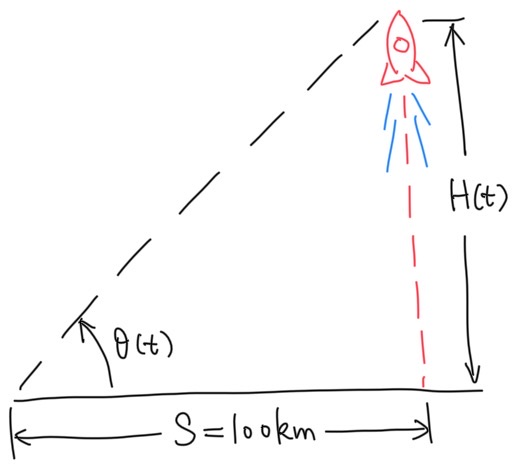
\includegraphics[width=5cm]{./images/ch2/Rocket.jpg}
		\column{0.6\textwidth}
		\pause 火箭的高度$H(t)=S\tan\theta(t)$,由此可知
		$$H'(t)=S\sec^2\theta(t)\theta'(t),$$
		\pause 将$S=100$,$\theta(t)=\df{\pi}4$,$\theta'(t)=0.1$代入即得
		指定时刻火箭上升的速率为$20$km/s。\hfill$\Box$
	\end{columns}
\end{frame}

\begin{frame}
	\linespread{1.5}
	\ba{3.长度为$6$米的梯子靠在墙角,梯子底部距离墙角$5$米,某一时刻梯子底部开始
	向远离墙角的方向滑动,滑动的速度为$0.2$米每秒,问
	\begin{enumerate}[(1)]
	  \setlength{\itemindent}{1cm}
	  \item 此时梯子顶部下滑的速度是多少?
	  \item 由梯子、墙面和地面构成的三角形的面积随时间的变化率是多少?
	  \item 梯子和地面的夹角的以怎样的速率变化?
	\end{enumerate}}	
\end{frame}

\begin{frame}
	\linespread{1.5}
	\small 解:\it
	如图,
	\begin{columns}
		\column{0.4\textwidth}
		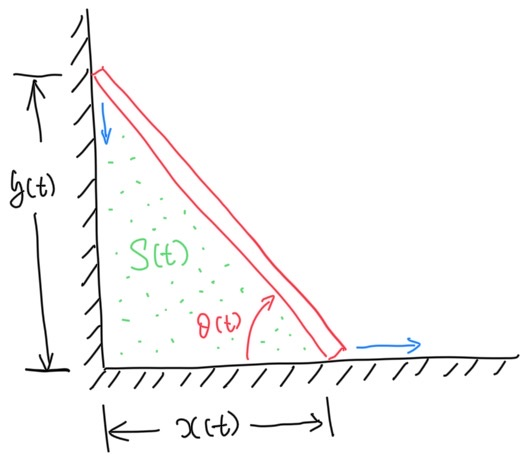
\includegraphics[width=5cm]{./images/ch2/ladder.jpg}
		\column{0.6\textwidth}
		\pause (1)显然$x^2(t)+y^2(t)=36$,两边求导可得
		$x'(t)x(t)+y'(t)y(t)=0$,进而
		$$y'(t)=-\df{x'(t)x(t)}{y(t)},$$
		\pause 代入$x(t)=5,x'(t)=0.2,y(t)=\sqrt{11}$,可得指定时刻
		梯子顶部的下滑速度为$-\df1{\sqrt{11}}$m/s;
	\end{columns}
\end{frame}

\begin{frame}
	\linespread{1.5}
	\small 解:\it
	如图,
	\begin{columns}
		\column{0.4\textwidth}
		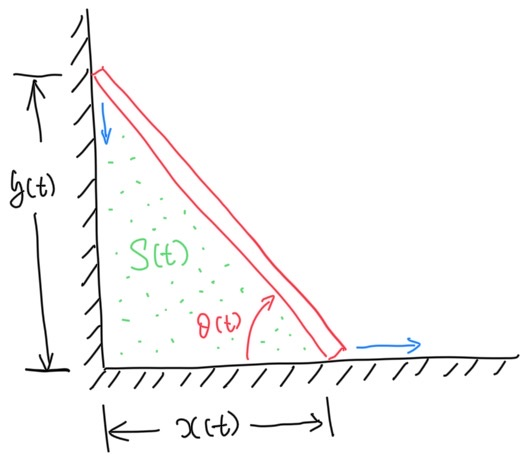
\includegraphics[width=5cm]{./images/ch2/ladder.jpg}
		\column{0.6\textwidth}
		(2)$S(t)=\df12x(t)y(t)$,故
		$$S'(t)=\df12[x'(t)y(t)+x(t)y'(t)],$$
		\pause 代入$x(t)=5,x'(t)=0.2,y(t)=\sqrt{11},y'(t)=-\df1{\sqrt{11}}$,
		可得所求三角形面积的变化速率为$-\df{7}{5\sqrt{11}}$m$^2$/s;
	\end{columns}
\end{frame}

\begin{frame}
	\linespread{1.5}
	\small 解:\it
	如图,
	\begin{columns}
		\column{0.4\textwidth}
		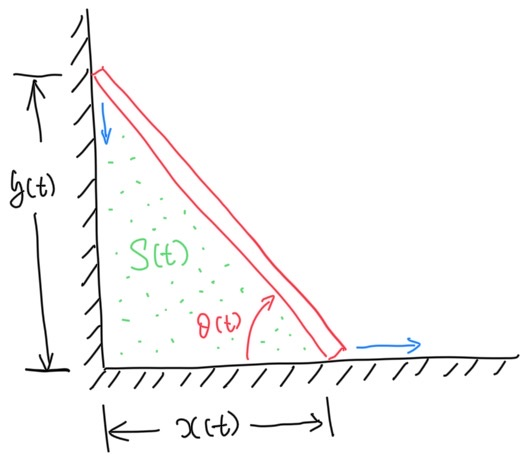
\includegraphics[width=5cm]{./images/ch2/ladder.jpg}
		\column{0.6\textwidth}
		(3)$\theta(t)=\arctan\df{y(t)}{x(t)}$,故
		$$\theta'(t)=\df1{1+\frac{y^2(t)}{x^2(t)}}
		=\df{y'(t)x(t)-y(t)x'(t)}{x^2(t)+y^2(t)},$$
		\pause 代入$x(t)=5,x'(t)=0.2,y(t)=\sqrt{11},y'(t)=-\df1{\sqrt{11}}$,
		可得指定时刻梯子和地面夹角的变化率为$-\df1{5\sqrt{11}}$弧度/s。\hfill$\Box$
	\end{columns}
\end{frame}

\begin{frame}
	\linespread{1.5}
	\ba{4.半径为$a$的圆球渐渐沉入盛有水的半径为$b(b>a)$的圆柱形容器中,若
	球的下降速度恒为$c$,求球浸没入水中恰好一半时,容器内水面上升的速率。
	}\pause
	
	\small 解:\it
	设$t$时刻,水中的球冠高度为$h(t)$,则此时水中的球冠体积
	$$V(t)=\df{\pi}3(3a-h(t))h^2(t),$$
	\pause 从而没入水中的球冠体积变换率
	$$V'(t)=\pi(2ah(t)-h^2(t))h'(t),$$
	\pause 相应地,桶内水面升高的速率为
	$$H'(t)=\df{V'(t)}{\pi [b^2-a^2+(a-h)^2]}
	=\df{2ah(t)-h^2(t)}{\pi [b^2-a^2+(a-h)^2]}h'(t),$$
	\pause 代入$h(t)=a,h'(t)=c$,即得所求水面上升的速率为$\df{a^2c}{b^2-a^2}$。
	\hfill$\Box$
\end{frame}

% % !Mode:: "TeX:UTF-8"

\titlepage

\begin{frame}{说在前面}
	\linespread{1.5}
	  \begin{itemize}[<+-|alert@+>]
	    \item 过往的作业不订正、不补齐的不予批改,打分不超过\,\ba{C}
	    \item 不交作业的默认记为\,\ba{D}
	    \item 需要换作业本的,请“移植”照片,写清楚个人信息
	    \item 请自行完成SPOC课程中的测试
	    \item 第二次单元测试即将发布,成绩记入期末总成绩
	  \end{itemize}
\end{frame}

\begin{frame}{出现的问题}
	\linespread{1.5}
	  \begin{itemize}[<+-|alert@+>]
	    \item 用中值定理证明
	    \begin{itemize}
	      \item \it 写清楚理论依据:\b 由\ldots 定理 
	      \item \it 注意陈述的完整性:\b 存在$\xi\in(a,b)$
	      \item \it 注意语序:强烈建议不要从结果说起,写得像分析过程
	    \end{itemize}
	    \item 数学符号的书写
	    \begin{itemize}
	      \item \it 希腊字母:\b $\xi$像$\e$,$\eta$像$n$,$\mu$像$u$
	      \item \b\it $\ln 2$写成了$\ln^2$
	      \item \it 微分的表示:\b $1+\ln2\d x$和$(1+\ln2)\d x$不同!
	    \end{itemize}
	  \end{itemize}
\end{frame}

\section{2.6 微分}

\begin{frame}
	\linespread{1.5}
	\ba{1.设$y=x^3-2x$,
	\begin{enumerate}[(1)]
	  \setlength{\itemindent}{1cm}
	  \item 计算在$x=2$处当$\Delta x$分别为$1,\;0.1,\;
	  0.01$时的$\Delta y$和$\d y$;
	  \item 写出$x=2$时$y$的微分表达式。
	\end{enumerate}}
	\pause
	
% 	\bigskip
	
	\small 解:\it
	\begin{align*}
		\Delta y&=[(x+\Delta x)^3-2(x+\Delta x)]-(x^3-2x)\\
		&=(3x^2-2)\Delta x+3x\Delta x^2+\Delta x^3,\\
		\d y&=(3x^2-2)\d x=(3x^2-2)\Delta x.
	\end{align*}
\end{frame}

\begin{frame}
	\linespread{1.5}
	
	\small\it 当$x=2$时,
	\begin{align*}
		\Delta y|_{x=2}&
		=10\Delta x+6\Delta x^2+\Delta x^3,\\
		\d y|_{x=2}&=10\Delta x.
	\end{align*}
	\pause 进而
	\begin{enumerate}[(i)]
	  \item 当$x=2,\Delta x=1$时,$\Delta y=17,\;\d y=10$;
	  \item 当$x=2,\Delta x=0.1$时,$\Delta y=1.061,\;\d y=1$;
	  \item 当$x=2,\Delta x=0.01$时,$\Delta y=0.100601,\;\d y=0.1$。
	\end{enumerate}
	\hfill$\Box$
\end{frame}

\begin{frame}
	\linespread{1.5}
	\ba{2.已知$2^{xy}=x-y$,求$\d y|_{x=0}$。
	}\pause
	
	\bigskip
	
	\small 解:\it 
	已知方程两边求微分,可得
	$$2^{xy}\ln2(x\d y+y\d x)=\d x-\d y,$$
	进而
	$$\d y=\df{1-y2^{xy}\ln2}{1+x2^{xy}\ln2}\d x.$$
	\pause $x=0$时,$y=-1$,带入即得
	$$\d y|_{x=0}=(1+\ln2)\d x.$$
	\hfill$\Box$
\end{frame}

\begin{frame}
	\linespread{1.5}
	\ba{5.已知当$h\to 0$时,
	$$f(x+2h)-f(x)=h\sqrt{x^2+2x}+\circ(h),$$
	求$\d\left[f\left(\df1x\right)\right]$。}\pause

	\bigskip
	
	\small 解: \it 
	由已知
	$$\lim\limits_{h\to0}\df{f(x+2h)-f(x)}{2h}
	=\lim\limits_{h\to0}\df{h\sqrt{x^2+2x}+\circ(h)}{2h}
	=\df{\sqrt{x^2+2x}}2.
	$$
	也即$f'(x)=\df{\sqrt{x^2+2x}}2$,\pause 故
	$$\d\left[f\left(\df1x\right)\right]
	=f'\left(\df1x\right)\left(-\df1{x^2}\right)\d x
	=-\df{\sqrt{1+2x}}{2x^2|x|}\d x.$$
	\hfill$\Box$
\end{frame}

\begin{frame}
	\linespread{1.5}
	\ba{6.设$a>0$,$|x|<<a$(表示$|x|$远远小于$a$),证明近似公式
	$$\sqrt[n]{a^n+x}\approx a+\df{x}{na^{n-1}}.$$}\pause
	
	\bigskip
	
	\small 证:\it
	记$f(x)=\sqrt[n]{a^n+x}$,显然$f(0)=a$,
	又
	$$f'(x)=\df1n(a^n+x)^{\frac1n-1}\quad
	\Rightarrow f'(0)=\df1{na^{n-1}}.
	$$
	故由微分的几何意义,当$|x|<<a$时,总有
	$$\sqrt[n]{a^n+x}\approx f(0)+f'(0)x
	=a+\df{x}{na^{n-1}}.$$
	\hfill$\Box$
\end{frame}

\section{3.1 微分中值定理}

\begin{frame}
	\linespread{1.5}
	\ba{1.设$0<a<b$,$f(x)$在$[a,b]$上连续,在$(a,b)$内可导,证明:
	(1)$\exists\xi\in(a,b)$,使得:
	$f(b)-f(a)=\ln\df ba\cdot \xi f\,'(\xi)$}\pause
	
	\bigskip
	
	\small 证:\it
	注意到$f(x)$和$\ln x$在$[a,b]$上均连续,在
	在$(a,b)$内均可导,且$(\ln x)'=\df1x\ne 0$,故由Cauchy中值定理,
	存在$\xi\in(a,b)$,使得
	$$\df{f(b)-f(a)}{\ln b-\ln a}=\df{f'(\xi)}{\frac1{\xi}},$$
	整理后即证。\hfill$\Box$
\end{frame}

\begin{frame}
	\linespread{1.5}
	\ba{1.设$0<a<b$,$f(x)$在$[a,b]$上连续,在$(a,b)$内可导,证明:
	(2)$\exists\eta\in(a,b)$,使得:
    
    \centering $2\eta[f(b)-f(a)]=(b^2-a^2)f\,'(\eta)$
    
    }\pause
	
	\bigskip
	
	\small 证:\it
	注意到$f(x)$和$x^2$在$[a,b]$上均连续,在
	在$(a,b)$内均可导,且$(x^2)'=2x\ne 0$,故由Cauchy中值定理,
	存在$\eta\in(a,b)$,使得
	$$\df{f(b)-f(a)}{b^2-a^2}=\df{f'(\eta)}{2\eta},$$
	整理后即证。\hfill$\Box$
\end{frame}

\begin{frame}
	\linespread{1.5}
	\ba{1.设$0<a<b$,$f(x)$在$[a,b]$上连续,在$(a,b)$内可导,证明:
	(3)存在$x_1,x_2,x_3\in(a,b)$,使得
	
	\centering $f\,'(x_1)=(b+a)\df{f\,'(x_2)}{2x_2}=(a^2+ab+b^2)
	\df{f\,'(x_3)}{3x_3^2}$
    
    }\pause
	
	\bigskip
	
	\small 证:\it
	注意到$f(x)$和$x,x^2,x^3$在$[a,b]$上均连续,在
	在$(a,b)$内均可导,且$(x)'=x\ne 0,(x^2)'=2x\ne 0,
	(x^3)'=3x^2\ne 0$,故由Cauchy中值定理,
	存在$x_1,x_2,x_3\in(a,b)$,使得
	$$\df{f(b)-f(a)}{b-a}=f'(x_1),$$
	$$\df{f(b)-f(a)}{b^2-a^2}=\df{f'(x_2)}{2x_2}
	\quad\Rightarrow\quad
	\df{f(b)-f(a)}{b-a}=(b+a)\df{f'(x_2)}{2x_2},$$
	$$\df{f(b)-f(a)}{b^3-a^3}=\df{f'(x_3)}{3x_3^2}
	\quad\Rightarrow\quad
	\df{f(b)-f(a)}{b-a}=(a^2+ab+b^2)\df{f'(x_3)}{3x_3^2},$$
	整理后即证。\hfill$\Box$
\end{frame}

\begin{frame}
	\linespread{1.5}
	\ba{1.设$0<a<b$,$f(x)$在$[a,b]$上连续,在$(a,b)$内可导,证明:
	(4)若$f\,'(x)\ne 0$,则存在$\xi,\eta\in(a,b)$,使得
	
	\centering $\df{f'(\xi)}{f'(\eta)}=\df{e^b-e^a}{b-a}e^{-\eta}$
    
    }\pause
	
	\bigskip
	
	\small 证:\it
	由Lagrange和Cauchy中值定理,存在$\xi,\eta\in(a,b)$,使得
	$$\df{f(b)-f(a)}{b-a}=f'(\xi)
	\quad\Rightarrow\quad
	f(b)-f(a)=f'(\xi)(b-a).$$
	$$\df{f(b)-f(a)}{e^b-e^a}=\df{f'(\eta)}{e^{\eta}}
	\quad\Rightarrow\quad
	f(b)-f(a)=\df{e^b-e^a}{e^{\eta}}f'(\eta).$$
	整理后即证。\hfill$\Box$
\end{frame}

\begin{frame}
	\linespread{1.5}
	\ba{1.设$0<a<b$,$f(x)$在$[a,b]$上连续,在$(a,b)$内可导,证明:
	(5)存在$c\in(a,b)$,使得
	
	\centering $\df{1}{a-b}\left|\begin{array}{cc}
	a & b\\ f(a) & f(b)
	\end{array}\right|=f(c)-cf'(c).$
    
    }\pause
	
	\bigskip
	
	\small 证:\it
	由Cauchy中值定理,存在$c\in(a,b)$,使得
	\begin{align*}
		\df{1}{a-b}\left|\begin{array}{cc}
		a & b\\ f(a) & f(b)
		\end{array}\right|
		&=\df{af(b)-bf(a)}{a-b}=\df{\frac{f(b)}b-\df{f(a)}a}{\frac1b-\frac1a}\\
		&=\df{\left(\frac{f(x)}x\right)'_{x=c}}{\left(\frac1x\right)'_{x=c}}
		=f(c)-cf'c.
	\end{align*}
	即证。\hfill$\Box$
\end{frame}

\begin{frame}
	\linespread{1.5}
	\ba{1.设$0<a<b$,$f(x)$在$[a,b]$上连续,在$(a,b)$内可导,证明:
	(6)若$f(a)=0$,则存在$\mu\in(a,b)$,使得
	
	\centering $f'(\mu)=\df{a}{a+b-2\mu}f(\mu).$
    
    }\pause
	
	\bigskip
	
	\small 证:\it
	令$F(x)=f(x)\left(\df{a+b-2x}2\right)^{\frac a2}$,可以验证
	$F(x)$在$\left[a,\df{a+b}2\right]$上满足Rolle定理条件,故存在
	$\mu\in\left(a,\df{a+b}2\right)\subset(a,b)$,使得
	$$F'(\mu)=\left(\df{a+b-2\mu}2\right)^{\frac a2-1}
	\left[f'(\mu)\left(\df{a+b-2\mu}2\right)
	-f(\mu)a\right]=0,$$
	$\left(\df{a+b-2\mu}2\right)^{\frac a2-1}\ne0$,故必有
	$f'(\mu)\left(\df{a+b-2\mu}2\right)-f(\mu)\df a2=0,$
	即证。\hfill$\Box$
\end{frame}

\begin{frame}
	\linespread{1.5}
	\ba{2.$f(x)\in C^1[a,b]$,$f(a)=f(b)=0$,$f'_+(a)f'_-(b)>0$,
	证明:$f(x)$在$(a,b)$内至少有一个零点。}\pause
	
	\bigskip
	
	\small 证:\it
	不妨设$f'_+(a)>0,f'_-(b)<0$。由$f'_+(a)>0$可知,存在$\delta_1>0$,
	使对任意$x\in(a,a+\delta_1)$,总有
	$$\df{f(x)-f(a)}{x-a}>0\quad\Rightarrow
	\quad f(x)=f(x)-f(a)>0.$$
	因此可以取到某个$x_1\in(a,b)$,使得$f(x_1)>0$。
	
	\pause 类似地,由$f'_-(b)<0$,可知比存在某个$x_2\in(a,b)$,使得$f(x_2)<0$。
	
	\pause 至此,由介值定理,必存在某个$\xi$介于$x_1$和$x_2$之间,使得$f(\xi)=0$。
	\hfill$\Box$
\end{frame}

\begin{frame}
	\linespread{1.5}
	\ba{3.证明:对任意$x>1$,
	
	\centering $(x^2-1)\ln x\geq(x-1)^2$。
	
	}\pause
	
	\bigskip
	
	\small 证:\it
	由Lagrange中值定理,存在$\xi$介于$x$和$1$之间,使得
	$$\df{\ln x-\ln 1}{x-1}=\df1{\xi},$$
	\pause 显然$0<\xi<x+1\Rightarrow\df1{\xi}>\df1{x+1}$,带入前式整理后即证。
	\hfill$\Box$
\end{frame}

\begin{frame}
	\linespread{1.5}
	\ba{4.$e<a<b<e^2$,证明:$\ln^2b-\ln^2a>\df2{e^2}(b-a)$。}\pause
	
	\bigskip
	
	\small 证:\it
	由Lagrange中值定理,存在$\xi\in(a,b)$,使得
	$$\df{\ln^2b-\ln^2a}{b-a}=\df{2\ln\xi}{\xi},$$
	注意到$e<\xi<e^2$,故
	$$1<\ln\xi<2,\quad \xi<e^2,$$
	故
	$\df{2\ln\xi}{\xi}>\df2{e^2},$
	代入前式整理即证。
	\hfill$\Box$
\end{frame}

\begin{frame}
	\linespread{1.5}
	\ba{5.$f(x)$在$x>0$二阶可导,$f''(x)>0$,令$u_n=f(n)\;
	 (n\in\mathbb{Z}_+)$,证明:若$u_1<u_2$,则$\{u_n\}$必发散;
	问:若$u_1>u_2$,$\{u_n\}$是否必收敛?(若正确,证明之;否则给出反例。)}\pause
	
	\bigskip
	
	\small 证:\it
	由$f''(x)>0$可知,$f'(x)$单调递增。若$u_1<u_2$,也即$f(1)<f(2)$,
	由Lagrange中值定理,存在$\xi_1\in(1,2)$,使得
	$$0<\df{f(2)-f(1)}{2-1}=f'(\xi_1),$$
	进而可知对任意$x>2$,均有$f'(x)>f'(\xi_1)$。
\end{frame}

\begin{frame}
	\linespread{1.5}
% 	\ba{5.$f(x)$在$x>0$二阶可导,$f''(x)>0$,令$u_n=f(n)\;
% 	 (n\in\mathbb{Z}_+)$,证明:若$u_1<u_2$,则$\{u_n\}$必发散;
% 	问:若$u_1>u_2$,$\{u_n\}$是否必收敛?(若正确,证明之;否则给出反例。)}\pause
	
% 	\bigskip
	
	\small \it
	对任意$n\geq2$,由Lagrange中值定理,存在$\xi_n\in(n,n+1)$,使得
	$$\df{f(n+1)-f(n)}{(n+1)-n}=f'(\xi_n)>f'(\xi_1)$$
	进而可得
	$$
	f(n+1)>f(n)+f'(\xi_1)>f(n-1)+2f'(\xi_1)>\ldots>f(1)+nf'(\xi_1),
	$$
	由此显然可知$\{u_n\}$发散。
	
	若$u_1>u_2$,$\{u_n\}$未必收敛。例如:$f(x)=(x-3)^2$,其中$u_1=4>1=u_2$,
	但显然$\{(n-3)^2\}$发散。\hfill$\Box$
\end{frame}

% % !Mode:: "TeX:UTF-8"

\titlepage

% \begin{frame}{说在前面}
% 	\linespread{1.5}
% 	  \begin{itemize}[<+-|alert@+>]
% 	    \item 过往的作业不订正、不补齐的不予批改,打分不超过\,\ba{C}
% 	    \item 不交作业的默认记为\,\ba{D}
% 	    \item 需要换作业本的,请“移植”照片,写清楚个人信息
% 	    \item 请自行完成SPOC课程中的测试
% 	    \item 第二次单元测试即将发布,成绩记入期末总成绩
% 	  \end{itemize}
% \end{frame}

\begin{frame}{需要注意的问题}
	\linespread{1.5}
	  \begin{itemize}%[<+-|alert@+>]
	    \item L'Hospital法则
	    \begin{itemize}
	      \item \it 只能应用于“$\df{\bm{0}}{\bm{0}}$”
	      和“$\df{\bm{\infty}}{\bm{\infty}}$”型
	      \item \it 及时使用无穷小代换进行简化
	      \item \it 不正规的符号:\b 
	      $\xlongequal{\footnotesize\mbox{“L”}}$、
	      $\xlongrightarrow{\footnotesize\mbox{“L'Hospital法则”}}$、
	      $\df{\bm{0}}{\bm{0}}$、$\df{\bm{\infty}}{\bm{\infty}}$
	    \end{itemize}
	    \item Taylor公式
	    \begin{itemize}
	      \item \it Taylor多项式不包含余项
	      \item \it 合并同次幂的系数
	      \item \it 尽量按照幂次由低到高排列,最后写余项
	    \end{itemize}
	  \end{itemize}
\end{frame}

\begin{frame}{出现的问题}
	\linespread{1.5}
	  \begin{itemize}%[<+-|alert@+>]
	    \item 奇特的无穷小代换
	    \begin{itemize}
	      \item \it\b $\ln\tan7x\sim\ln7x$
	      \item \it\b $\ln\tan7x\sim\tan7x$
	      \item \it\b $(1+x)^{\frac1x}\sim e$
	    \end{itemize}
	    \item 奇特的Taylor展开
	    \begin{itemize}
	      \item \it \b$\sum\limits_{k=0}^n
	      \df{(-1)^k(x-3)^k}{(x-1)^{k+1}}+\circ((x-3)^n)$
	      \item \b $\sqrt{\sum\limits_{k=0}^n\left(\df{x^2}4\right)^k
	      +\circ(x^{2n})}$
	    \end{itemize}
	  \end{itemize}
\end{frame}

\section{3.2 L'Hospital法则}

\begin{frame}
	\linespread{1.5}
	\ba{1.计算如下极限:}
	\pause
	
% 	\bigskip
	
	\small 解:
	(1)$\limx{0^+}\df{\ln\tan 7x}{\ln\sin 3x}=\limx{0^+}\df{\df{7\sec^27x}{\tan7x}}{\df{3\sec^23x}{\tan3x}}
	=\limx{0^+}\df{\df7{7x}}{\df3{3x}}=1.$
	
	\pause	
	(2)$\limx{+\infty}\df{\ln\left(1+\df1x\right)}{\arctan x}
	=\df{\limx{+\infty}\ln\left(1+\df1x\right)}{\limx{+\infty}\arctan
	x}=\df{0}{\frac{\pi}2}=0.$
	
	\ba{注:$0/1$型,不能使用L'Hospital法则!}
	
	\pause	
	(3)$\limx{0^+}x^{\sin x}=\exp\left(\limx{0^+}\sin x\ln x\right)
	=\exp\left(\limx{0^+}x\ln x\right)$
	
	\quad$=\exp\left(\limx{0^+}\ln x^x\right)
	=1.$
	
	\pause
	(4)$\limx{\infty}x^2e^{\frac1{x^2}}$极限不存在。

	\ba{注:$\infty\cdot 1$型,不能使用L'Hospital法则!}
\end{frame}

\begin{frame}
	\linespread{1.5}
% 	\ba{1.计算如下极限:}
% 	\pause
	
% 	\bigskip
	
 	\small 	
	(5)$\limx{\infty}\df{x^2-\cos x}{x^2+\sin x}
	=\limx{\infty}\df{1-\frac{\cos x}{x^2}}{1+\frac{\sin x}{x^2}}=1.$
	
	\ba{注:第二个等号不能使用L'Hospital法则!}
	
	\pause	
	(6)$\limx{0}\df{x^2-\sin x}{x^2+\cos x}
	=\df{\limx{0}x^2-\limx{0}\sin x}{\limx{0}x^2+\limx{0}\cos x}=0.$
	
	\ba{注:$0/1$型,不能使用L'Hospital法则!}
	
	\pause
	(7)$\limx{0}\df{\ln(1+x^2)}{\sec x-\cos x}
	=\limx{0}\df{x^2\cos x}{1-\cos^2 x}
	=\limx{0}\df{x^2}{\sin^2 x}=1.$
	
	\pause
	(8)$\limx{0}\df{(1+x)^{1/x}-e}{x}
	=e\limx{0}\df{e^{1/x\ln(1+x)-1}-1}{x}$
	
	\quad$=e\limx{0}\df{1/x\ln(1+x)-1}{x}
	=e\limx{0}\df{\ln(1+x)-x}{x^2}$
	
	\quad$=e\limx{0}\df{\frac1{1+x}-1}{2x}
	=\frac e2\limx{0}\df{-1}{1+x}=-\frac e2.$
\end{frame}

\begin{frame}
	\linespread{1.5}
% 	\ba{1.计算如下极限:}
% 	\pause
	
% 	\bigskip
	
 	\small 
	(9)$\limx{1}(1-x^2)\tan\df{\pi}{2}x
	=2\limx{1}(1-x)\tan\df{\pi}{2}x
	$
	
	$\quad=2\lim\limits_{y\to0}y\tan\left[\df{\pi}2(1-y)\right]
	=2\lim\limits_{y\to0}\df y{\tan\left(\df{\pi}2y\right)}
	=\df4{\pi}.$
	
	\pause	
	(10)$\limx{0}\left(\df 1{x^2}-\df 1{x\tan x}\right)
	=\limx{0}\df {\tan x-x}{x^2\tan x}
	=\limx{0}\df {\tan x-x}{x^3}$
	
	$\quad
	=\limx{0}\df {\sec^2 x-1}{3x^2}
	\limx{0}\df {\tan^2 x}{3x^2}=\df13.$
	
	\pause	
	(11)$\limx{0}(x^2+2^x)^{1/x}
	=\exp\left[\limx{0}\df{\ln(x^2+2^x)}x\right]
	$
	
	$\quad=\exp\left[\limx{0}\df{2x+2^x\ln 2}{x^2+2^x}\right]
	=\exp\left[\limx{0}\df{2+2^x\ln^2 2}{2x+2^x\ln2}\right]$
	
	$\quad
	=\exp\left[\limx{0}\df{2^x\ln^3 2}{2+2^x\ln^22}\right]
	=\exp\left[\limx{0}\df{\ln^3 2}{\frac2{2^x}+\ln^22}\right]
	$
	
	$\quad
	=e^{\ln 2}=2.$
\end{frame}

\begin{frame}
	\linespread{1.5}
% 	\ba{1.计算如下极限:}
% 	\pause
	
% 	\bigskip
	
 	\small 
	(12)$\limx0\df{e^{\tan x}-e^x}{\tan x-x}
	=\limx0\df{e^{\tan x-x}-1}{\tan x-x}\limx0e^x
	=\limx0\df{\tan x-x}{\tan x-x}=1.$
	
	\bigskip
	\pause
	(13)$\limx{0}\left(\cot x-\df 1x\right)
	=\limx{0}\df{x-\tan x}{x\tan x}
	=\limx{0}\df{x-\tan x}{x^2}$
	
	$\hspace{1cm}
	=\limx{0}\df{1-\sec^2 x}{2x}
	=\limx{0}\df{-\tan^2 x}{2x}=0$
\end{frame}

\begin{frame}
	\linespread{1.5}
% 	\ba{1.计算如下极限:}
% 	\pause
	
% 	\bigskip
	
 	\small
	(14)\it $\limx{\infty}\left[\df1n\left(a_1^{\frac1x}+a_2^{\frac1x}
	+\ldots+a_n^{\frac1x}\right)\right]^{nx}$,其中$a_1,a_2,\ldots,a_n>0$
	
	记$A_n=\df{\left(a_1^{\frac1x}-1\right)+\left(a_2^{\frac1x}-1\right)
	+\ldots+\left(a_n^{\frac1x}-1\right)}n$,显然$\limx{\infty}A_n=0$。
	
	\pause
	\begin{align*}
		&\mbox{原式}
		=\limx{\infty}(1+A_n)^{\frac{1}{A_n}A_nnx}
		=\left[\limx{\infty}(1+A_n)^{\frac{1}{A_n}}\right]
		^{\limx{\infty}A_nnx}\\
		&=\exp\left\{\limx{\infty}x\left[\left(a_1^{\frac1x}-1\right)
		+\left(a_2^{\frac1x}-1\right)+\ldots+\left(a_n^{\frac1x}-1\right)\right]\right\}\\
		&=\exp\left[\limx{\infty}x\left(a_1^{\frac1x}-1\right)
		+\limx{\infty}x\left(a_2^{\frac1x}-1\right)
		+\ldots+\limx{\infty}x\left(a_n^{\frac1x}-1\right)\right]\\
		&=\exp\left(\limx{\infty}\df{x\ln a_1}{x}
		+\limx{\infty}\df{x\ln a_2}{x}
		+\ldots+\limx{\infty}\df{x\ln a_n}{x}\right)\\
		&=a_1a_2\ldots a_n.
	\end{align*}
\end{frame}

\begin{frame}
	\linespread{1.5}
	\ba{2.设$x\to 0$时,$x-\sin ax$与$x^2\ln(1-bx)$为等价无穷小,求$a,b$的值。
	}\pause
	
	\bigskip
	
	\small 解:\it 
	$x\to 0$时,$x^2\ln(1-bx)\sim-bx^3$,故必有
	$$\b 1=\limx0\df{x-\sin ax}{-bx^3}
	=\limx0\df{1-a\cos ax}{-3bx^2},$$
	右侧极限存在当且仅当$a=1$,进而
	$$1=\limx0\df{x-\sin ax}{-bx^3}
	=\limx0\df{1-\cos x}{-3bx^2}
	=\limx0\df{\frac{x^2}2}{-3bx^2}=-\df1{6b},$$
	故$b=-\df16$。\hfill$\Box$
	
	\pause\ba{正确的作法应使用Taylor公式!}
\end{frame}

\begin{frame}
	\linespread{1.5}
	\ba{2.设$x\to 0$时,$x-\sin ax$与$x^2\ln(1-bx)$为等价无穷小,求$a,b$的值。
	}\pause
	
	\bigskip
	
	\small 正解:\it 
	$x\to 0$时,$x^2\ln(1-bx)\sim-bx^3$。又由Taylor公式,
	$$x-\sin ax=x-ax+\df{a^3x^3}6+\circ(x^3),$$
	故
	\begin{align*}
		1&=\limx0\df{x-\sin ax}{-bx^3}
		=\limx0\df{(1-a)x+\df{a^3x^3}6+\circ(x^3)}{-bx^3}\\
		&=\limx0\df{1-a}{-bx^2}-\df{a^3}{6b},
	\end{align*}
	上式最后的极限存在当且仅当$1-a=0$,进而可知必有
	$a=1,b=-\df16$。\hfill$\Box$
\end{frame}

\section{3.2 Taylor公式}

\begin{frame}
	\linespread{1.5}
	\ba{1.求$f(x)=x^4+x^3-2x-4$在$x=0$和$x=2$处的三阶Taylor多项式。}\pause

	\bigskip
	
	\small 解: \it 
	$f(x)$在$x=0$处的三阶Taylor多项式为
	$$P^{[0]}_3(x)=x^3-2x-4.$$
	\pause 又
	\begin{align*}
		f(x)&=[(x-2)+2]^4+[(x-2)+2]^3-2[(x-2)+2]-4\\
		&=(x-2)^4+9(x-2)^3+30(x-2)^2+42(x-2)+16,
	\end{align*}
	$f(x)$在$x=2$处的三阶Taylor多项式为
	$$P^{[2]}_3(x)=9(x-2)^3+30(x-2)^2+42(x-2)+16.$$
	\hfill$\Box$
\end{frame}

\begin{frame}
	\linespread{1.5}
	\ba{2.求函数$f(x)=\df1{x-1}$按$(x-3)$的幂展开的带有Peano余项的
	$n$阶Taylor公式。}\pause
	
	\bigskip
	
	\small 解:\it
	\begin{align*}
		f(x)&=\df1{2+(x-3)}=\df12\cdot\df1{1+\frac{x-3}2}\\
		&=\df12\left[\sum\limits_{k=0}^n\left(-\df{x-3}2\right)^k
		+\circ\left(\left(-\df{x-3}2\right)^n\right)\right]\\
		&=\sum\limits_{k=0}^n\df{(-1)^k(x-3)^k}{2^{k+1}}+\circ((x-3)^n).
	\end{align*}
	\hfill$\Box$
\end{frame}

\begin{frame}
	\linespread{1.5}
	\ba{3.求如下函数带Peano余项的Maclaurin公式}\pause
	
	\bigskip
	
	\small 解:(1)
	\begin{align*}
		\ln(2+x^2)&=\ln2+\ln\left(1+\df{x^2}2\right)\\
		&=\ln2+\sum\limits_{k=1}^n\df{(-1)^{k-1}\left(\frac{x^2}{2}\right)^k}{k}
		+\circ\left(\left(\df{x^2}{2}\right)^n\right)\\
		&=\ln2+\sum\limits_{k=1}^n\df{(-1)^{k-1}x^{2k}}{k2^k}
		+\circ(x^{2n}).
	\end{align*}
\end{frame}

\begin{frame}
	\linespread{1.5}
% 	\ba{3.求如下函数带Peano余项的Maclaurin公式}\pause
	
% 	\bigskip
	
	\small (2)
	$
		e^{\frac{x^2}2}
		=\sum\limits_{k=0}^n\df{\left(\frac{x^2}2\right)^k}{k!}
		+\circ\left(\left(\df{x^2}2\right)^n\right)
		=\sum\limits_{k=0}^n\df{x^{2k}}{k!2^k}
		+\circ\left(x^{2n}\right).
	$
	\bigskip
	
	\pause
	(3)
	$
		x\cos x^2
		=x\left[\sum\limits_{k=0}^n\df{(-1)^kx^{4k}}{(2k)!}
		+\circ(x^{2n})\right]$
		
		\quad $
		=\sum\limits_{k=0}^n\df{(-1)^kx^{4k+1}}{(2k)!}
		+\circ(x^{4n+1}).
	$
	\bigskip
	
	\pause
	(4)
	$
		\df{1+x^2}{1-x^2}
		=-1+\df2{1-x^2}
		=-1+2\left[\sum\limits_{k=0}^n(x^2)^k-\circ(x^{2n})\right]$
		
		\quad$
		=-1+\sum\limits_{k=0}^n2x^{2k}+\circ(x^{2n}).
	$
\end{frame}

\begin{frame}
	\linespread{1.5}
% 	\ba{3.求如下函数带Peano余项的Maclaurin公式}\pause
	
% 	\bigskip
	
	\small (5)
	\begin{align*}
		\df1{\sqrt{4-x^2}}
		&=\df12\left(1-\frac{x^2}4\right)^{-\frac12}\\
		&=\df12\left[\sum\limits_{k=0}^n\left(\begin{array}{c}
			-\frac12 \\ k
		\end{array}\right)\left(-\df{x^2}{4}\right)^k
		+\circ\left(\left(-\df{x^2}{4}\right)^n\right)
		\right]\\
		&=\sum\limits_{k=0}^n\df{(2k+1)!!}{k!8^k2}x^{2k}
		+\circ(x^{2n}).
	\end{align*}
	
	\pause
	(6)
	\begin{align*}
		&\sin^2x-x^3=\df12-\df12\cos2x-x^3\\
% 		&=\df12-\df12\left[1-\df{(2x)^2}{2!}+\df{(2x)^4}{4!}
% 		+\ldots+\df{(-1)^k(2x)^{2k}}{(2k)!}+\circ((2x)^{2n})\right]-x^3\\
		&=x^2-x^3-\df{2^3x^4}{4!}
		+\ldots-\df{(-1)^k2^{2k-1}x^{2k}}{(2k)!}+\circ(x^{2n}).
	\end{align*}
\end{frame}

\begin{frame}
	\linespread{1.5}
% 	\ba{3.求如下函数带Peano余项的Maclaurin公式}\pause
	
% 	\bigskip
	
	\small (7)\it 注意到$(1+x)e^x=(xe^x)'$,而
	$$xe^x=x\sumn\df{x^n}{n!}=\sumn\df{x^{n+1}}{n!},$$
	故
	$$(1+x)e^x=\left[\sumn\df{x^{n+1}}{n!}\right]'
	=\sumn\df{(x^{n+1})'}{n!}
	=\sumn\df{(n+1)x^n}{n!},$$
	于是所求带Peano余项的Maclaurin公式为
	$$(1+x)e^x=\sum\limits_{k=0}^n\df{(k+1)x^k}{k!}+\circ(x^{n+1}).$$
	\hfill$\Box$
\end{frame}

% % !Mode:: "TeX:UTF-8"

\titlepage

% \begin{frame}{说在前面}
% 	\linespread{1.5}
% 	  \begin{itemize}[<+-|alert@+>]
% 	    \item 过往的作业不订正、不补齐的不予批改,打分不超过\,\ba{C}
% 	    \item 不交作业的默认记为\,\ba{D}
% 	    \item 需要换作业本的,请“移植”照片,写清楚个人信息
% 	    \item 请自行完成SPOC课程中的测试
% 	    \item 第二次单元测试即将发布,成绩记入期末总成绩
% 	  \end{itemize}
% \end{frame}

% \begin{frame}{需要注意的问题}
% 	\linespread{1.5}
% 	  \begin{itemize}%[<+-|alert@+>]
% 	    \item L'Hospital法则
% 	    \begin{itemize}
% 	      \item \it 只能应用于“$\df{\bm{0}}{\bm{0}}$”
% 	      和“$\df{\bm{\infty}}{\bm{\infty}}$”型
% 	      \item \it 及时使用无穷小代换进行简化
% 	      \item \it 不正规的符号:\b 
% 	      $\xlongequal{\footnotesize\mbox{“L”}}$、
% 	      $\xlongrightarrow{\footnotesize\mbox{“L'Hospital法则”}}$、
% 	      $\df{\bm{0}}{\bm{0}}$、$\df{\bm{\infty}}{\bm{\infty}}$
% 	    \end{itemize}
% 	    \item Taylor公式
% 	    \begin{itemize}
% 	      \item \it Taylor多项式不包含余项
% 	      \item \it 合并同次幂的系数
% 	      \item \it 尽量按照幂次由低到高排列,最后写余项
% 	    \end{itemize}
% 	  \end{itemize}
% \end{frame}

\begin{frame}{出现的问题}
	\linespread{1.5}
	  \begin{itemize}%[<+-|alert@+>]
	    \item 错误的推导
	    \begin{itemize}
	      \item \it\b $F(x)=\df{f(x)-f(a)}{x-a}=f'(\xi)\;\Rightarrow\;
	      F'(x)=f''(\xi)$
	      \item \it\b $\limx0\df{f''(x)}{|x|}=0\;\Rightarrow\; f''(0)=|x|=0$
	      \item \it\b $\limx0\df{f''(x)}{|x|}=0\;\Rightarrow\; f''(x)=|x|>0$
	      \item \it\b $\limx{a}F(x)=f'(x)$\pause
	    \end{itemize}
	    \item 自己发明的符号和说法
	    \begin{itemize}
	      \item \it\b $g''|_{x\to\frac12^+}$
	      \item \it\b $R((x-3)^n)$
	      \item \it\b $f(x)$在$x\to0^-$递减,在$x\to0^+$递增
	    \end{itemize}
	  \end{itemize}
\end{frame}

\section{3.3 Taylor公式}

\begin{frame}
	\linespread{1.5}
	\ba{4.计算如下极限:}
	\pause
	
% 	\bigskip
	
	\small 解:
	(1)$\limx{+\infty}(\sqrt[3]{x^3+3x^2}-\sqrt[4]{x^4-2x^3})$
	
	\quad$=\limx{+\infty}x\left(\sqrt[3]{1+\frac3x}
	-\sqrt[4]{1-\frac2x}\right)
	\quad =\lim\limits_{y\to0}\df{\sqrt[3]{1+3y}
	-\sqrt[4]{1-2y}}{y}$
	
	\quad$=\lim\limits_{y\to0}\df{1+\frac133y-1-\frac14(-2y)+\circ(y)}y=\df32$
	
	\pause	
	(2)$\limx0\df{\cos x-e^{-\frac{x^2}2}}{x^2[x+\ln(1-x)]}$
	
	\quad$=\limx0\df{1-\frac{x^2}2+\frac12\frac{x^4}{4!}-1+\frac{x^2}2
	-\frac{x^4}{4}+\circ(x^4)}{x^2(x+(-x)-\frac{x^2}2+\circ(x^2))}
	=\df16$
	
	\pause
	(3)
	$\limx0\df{1+\frac12x^2-\sqrt{1+x^2}}{(\cos x-e^{x^2})\sin x^2}$
	
	\quad$=\limx0\df{1+\frac12x^2-\left(1+\frac12x^2-\frac18x^4+\circ(x^4)\right)}
	{\left(1-\frac{x^2}2-1-x^2+\circ(x^2)\right)x^2}=-\df1{12}.$
\end{frame}

\begin{frame}
	\linespread{1.5}
	\ba{4.计算如下极限:}
	\pause
	
% 	\bigskip
	
	\small 解:
	(4)$\limx{+\infty}\left[\left(x^3-x^2+\df{x}2\right)e^{\frac1x}
	-\sqrt{x^6+1}\right]$
	
	\quad$=\lim\limits_{y\to0^+}\df{\left(1-y+\frac12y^2
	\right)e^y-\sqrt{1+y^6}}{y^3}$
	
	\quad$=\lim\limits_{y\to0^+}\df{\left(1-y+\frac12y^2
	\right)\left(1+y+\frac{y^2}2+\frac{y^3}6+\circ(y^3)\right)
	-\left(1+\circ(y^3)\right)}{y^3}$
	
	\quad$=\lim\limits_{y\to0^+}\df{\frac16y^3+\circ(y^3)}{y^3}=\df16.$
\end{frame}

\begin{frame}
	\linespread{1.5}
	\ba{5.应用关于$(x-1)$的$3$阶Taylor公式计算$\sqrt[3]{2}$的近似值,并估计其误差。
	}\pause
	
	\bigskip
	
	\small 解:\it 
	由Taylor公式,存在$\xi$介于$1$和$x$之间,使得
	\begin{align*}
		&\sqrt[3]x=[1+(x-1)]^{\frac13}\\
		&=1+\df13(x-1)
		+\df13\cdot\df{-2}3\cdot\df{(x-1)^2}2
		+\df13\cdot\df{-2}3\cdot\df{-5}3\cdot\df{(x-1)^3}6\\
		&\quad+\df13\cdot\df{-2}3\cdot\df{-5}3\cdot\df{-8}3
		\cdot\df{\xi^{\frac13-4}}{4!}(x-1)^4\\
		&=1+\df{x-1}3-\df{(x-1)^2}9+\df{5(x-1)^3}{81}
		-\df{10(1+\xi)^{\frac13-4}}{243}(x-1)^4,
	\end{align*}
	
	\pause
	
	带入$x=2$即得
	$\sqrt[3]2\approx\df{104}{81},$
	注意到$1\leq\xi\leq 2$,故计算误差$\left|\df{10\xi^{\frac13-4}}{243}\right|
	\leq\df{10}{243}$。
	\hfill$\Box$
\end{frame}

\begin{frame}
	\linespread{1.5}
	\ba{5.应用$3$阶Taylor公式计算$\sqrt[3]{30}$的近似值,并估计其误差。
	}\pause
	
	\bigskip
	
	\small 解:\it 
	$\sqrt[3]{30}=3\sqrt[3]{1+\frac19}$,由Taylor公式,对任意$x>0$
	存在$\xi\in(0,x)$,使得
	$$(1+x)^{\frac13}=1+\df13x-\df19x^2+\df5{81}x^3
	-\df{10(1+\xi)^{\frac13-4}}{243}x^4,$$
	
	\pause
	带入$x=\frac19$,计算可得$\sqrt[3]{30}\approx\df{61160}{19683}\approx
	3.10725$,
	注意到$0<\xi<\frac19$,故计算误差
	$$3\left|\df{10(1+\xi)^{\frac13-4}}{243}
	\df1{9^4}\right|\leq3\left|\df{10}{243}\df1{9^4}\right|=\df{10}{531441}
	\approx 1.88\times10^{-5}.$$
	\hfill$\Box$
\end{frame}

\begin{frame}
	\linespread{1.5}
	\ba{6.已知$f(x)$在$x=0$附近二阶可导,且
	$$\limx0\left[\df{\sin x}{x^3}+\df{f(x)}{x^2}\right]=0,$$
	求$f(0),f'(0),f''(0)$。
	}\pause
	
	\bigskip
	
	\small 解:\it 
	由已知,可设
	$f(x)=f(0)+f'(0)x+\df{f''(0)}2x^2+\circ(x^2).$
	\pause
	于是
	\begin{align*}
		0&=\limx0\left[\df{\sin x}{x^3}+\df{f(x)}{x^2}\right]
		=\limx0\df{\sin x+xf(x)}{x^3}\\
		&=\limx0\df{x-\frac{x^3}6+xf(0)+x^2f'(0)+\frac{x^3}2f''(0)+\circ(x^3)}{x^3}\\
		&=\limx0\df{1+f(0)}{x^2}+\limx0\df{f'(0)}x+\df{f''(0)}2-\df16,
	\end{align*}
	
	\pause
	右端极限有意义,当且仅当
	$f(0)=-1,f'(0)=0,f''(0)=\frac13.$
	\hfill$\Box$
\end{frame}

\begin{frame}
	\linespread{1.5}
	\ba{7.证明:若在$(a,b)$内,$f''(x)>0$,则对任意$a<x_1<x_2<b$,恒有:
	对任意$\lambda\in(0,1)$,
	$$f(\lambda x_1+(1-\lambda)x_2)<\lambda
	f(x_1)+(1-\lambda)f(x_2).$$
	}
	
	\pause
	\small 证:\it 
	对任意$a<x_1<x_2<b$和任意$\lambda\in(0,1)$,
	记$x_{\lambda}=\lambda x_1+(1-\lambda)x_2$,则
	由Taylor公式,存在$\xi_1\in(x_1,x_{\lambda}),
	\xi_2\in(x_{\lambda},x_2)$,使得
	\begin{align*}
		f(x_1)&=f(x_{\lambda})-(1-\lambda)f'(x_{\lambda})(x_2-x_1)
		+(1-\lambda)^2\df{f''(\xi_1)}2(x_2-x_1)^2,\\
		f(x_2)&=f(x_{\lambda})+\lambda f'(x_{\lambda})(x_2-x_1)
		+\lambda^2\df{f''(\xi_2)}2(x_2-x_1)^2,
	\end{align*}
\end{frame}

\begin{frame}
	\linespread{1.5}
	\small \it 
	\begin{align*}
		f(x_1)&=f(x_{\lambda})-(1-\lambda)f'(x_{\lambda})(x_2-x_1)
		+(1-\lambda)^2\df{f''(\xi_1)}2(x_2-x_1)^2,\\
		f(x_2)&=f(x_{\lambda})+\lambda f'(x_{\lambda})(x_2-x_1)
		+\lambda^2\df{f''(\xi_2)}2(x_2-x_1)^2,
	\end{align*}
	
	\pause
	进而由$f''(x)>0$,可得
	\begin{align*}
		&\lambda f(x_1)+(1-\lambda)f(x_2)\\
		&=f(x_{\lambda})+(1-\lambda)^2\df{f''(\xi_1)}2(x_2-x_1)^2
		+\lambda^2\df{f''(\xi_2)}2(x_2-x_1)^2>f(x_{\lambda}).
	\end{align*}
	即证。
	\hfill$\Box$
\end{frame}

\begin{frame}
	\linespread{1.5}
	\ba{8.设在$f(x)$在$[0,a]$上二阶连续可导,
	$|f\,''(x)|\leq M$,且$|f(x)|$在$(0,a)$内可取到最大值,证明:
	$$|f\,'(0)+f\,'(a)|\leq Ma.$$	
	}
	
	\pause
	\vspace{-1em}
	\small 证:\it 
	设$x=c$为$f(x)$在$(0,a)$内的最大值点,则$f'(c)=0$。
	由Taylor公式,存在$\xi_1\in(0,c),\xi_2\in(c,a)$,使得
	\begin{align*}
		f'(0)&=f'(c)+f''(\xi_1)(0-c)=-f''(\xi_1)c,\\
		f'(a)&=f'(c)+f''(\xi_2)(1-c)=f''(\xi_2)(a-c),
	\end{align*}
	
	\pause 于是
	\begin{align*}
		|f'(0)+f'(a)|
		\leq|f''(\xi_1)|c+|f''(\xi_2)|(a-c)\leq M.
	\end{align*}
	\hfill$\Box$
\end{frame}

\section{3.4 函数的单调性与凹凸性}

\begin{frame}
	\linespread{1.5}
	\ba{1.证明下列不等式:(1)当$x\in(0,\pi/2)$时,$\sin x+\tan x>2x$。
	}
	
	\pause
	\small 证:\it 
		令$f(x)=\sin x+\tan x-2x$,则当$x\in(0,\pi/2)$时,
	$$f'(x)=\cos x+\sec^2x-2>\cos^2x+\sec^2x-2>0,$$
% 	记$u=\cos x$,当$x\in(0,\pi/2)$时,$u\in(0,1)$,记
% 	$g(u)=u-\df1{u^2}-2$,则
% 	$$u'(x)=1+\df2{u^3}>0,$$
% 	注意到$u(0)=0$,故当$u>0$时,恒有$g(u)>0$,也即$f'(x)>0$,
	\pause 又$f(0)=0$,故当$x\in(0,\pi/2)$时,必有$f(x)>0$。即证。
	\hfill$\Box$
\end{frame}

\begin{frame}
	\linespread{1.5}
	\ba{1.证明下列不等式:(2)当$x>0$时,$1+x\ln(x+\sqrt{1+x^2})>\sqrt{1+x^2}$。
	}
	
	\pause
	\small 证:\it 
	令$f(x)=1+x\ln(x+\sqrt{1+x^2})-\sqrt{1+x^2}$,则
	\begin{align*}
		f'(x)&=\ln(x+\sqrt{1+x^2})+\df{x(1+\frac{x}{\sqrt{1+x^2}})}
		{x+\sqrt{1+x^2}}-\df{x}{\sqrt{1+x^2}}\\
		&=\ln(x+\sqrt{1+x^2}),\\
		f''(x)&=\df{1+\frac{x}{\sqrt{1+x^2}}}{x+\sqrt{1+x^2}}=\df1{\sqrt{1+x^2}}>0,
	\end{align*}
	\pause 注意到$f'(0)=f(0)=0$,故由导数与函数单调性的关系可知,当$x>0$时,必有$f'(x)>0$,
	进而$f(x)>0$,即证。
	\hfill$\Box$
\end{frame}

\begin{frame}
	\linespread{1.5}
	\ba{3.设$x,y>0$,证明如下不等式:(2)$x\ln x+y\ln y\geq (x+y)\ln\df{x+y}2$
	}
	
	\pause
	\small 证:\it 
	考虑函数$f(x)=x^x$,则
	$$f'(x)=x^x(1+\ln x),\quad
	f''(x)=x^x(1+\ln x+\df1x).$$
	\pause 令$g(x)=1+\ln x+\df1x$,则
	$g'(x)=\df1x-\df1{x^2},$
	令$g'(x)=0$,可得$x=1$为其唯一驻点。当$x>1$时,$g'(x)>0$;
	当$x<1$时,$g'(x)<0$,故$x=1$为$g(x)$的最小值点。
	\pause 又$g(1)=0$,
	故当$x>0$时,总有$g(x)>0$,进而$f''(x)>0$,从而可知
	$f(x)$对应曲线是凹的。
	\pause 于是对任意$x,y>0$,必有
	$$\df{f(x)+f(y)}2>f\left(\df{x+y}2\right),$$
	带入其定义整理后即证。\hfill$\Box$
\end{frame}

\begin{frame}
	\linespread{1.5}
	\ba{4.设$f(x)$当$x\geq a$时二阶可导,且$f''(x)>0$,证明:
	$F(x)=\df{f(x)-f(a)}{x-a}$当$x>a$时单调递增。
	}
	
	\pause
	\small 证法一:\it 
	对任意$x>a$,
	$$F'(x)=\df{f'(x)(x-a)-[f(x)-f(a)]}{(x-a)^2}.$$
	令$h(x)=f'(x)(x-a)-[f(x)-f(a)]$,则$h'(x)=f''(x)(x-a)$,
	当$x>a$时,恒有$h'(x)>0$,又$h(a)=0$,故当$x>a$时,总有
	$h(x)>0$,进而可知$F'(x)>0$,从而当$x>a$时,$F(x)$单调递增。\hfill$\Box$
\end{frame}

\begin{frame}
	\linespread{1.5}
% 	\ba{4.设$f(x)$当$x\geq a$时二阶可导,且$f''(x)>0$,证明:
% 	$F(x)=\df{f(x)-f(a)}{x-a}$当$x>a$时单调递增。
% 	}
% 	
% 	\pause
	\small 证法二:\it 
	对任意$x>a$,
	$$F'(x)=\df{f'(x)(x-a)-[f(x)-f(a)]}{(x-a)^2}.$$
	又由Taylor公式,存在$\xi\in(a,x)$,
	$$f(a)=f(x)+f'(x)(a-x)+\df{f''(\xi)}2(a-x)^2
	>f(x)-f'(x)(x-a).$$
	从而
	$$f'(a)(x-a)-f(x)+f(a)>0.$$
	故由前式必有$F'(x)>0$,也即$F(x)$当$x>a$时,严格单调递增。\hfill$\Box$
\end{frame}

\section{3.5 函数的极值与最值}

\begin{frame}
	\linespread{1.5}
	\ba{1.求函数$f(x)=e^x+e^{-x}+\cos x$的极值。
	}
	
	\pause
	\small 解:\it 
	$$f'(x)=e^x-e^{-x}-\sin x,\quad f''(x)=e^x+e^{-x}-\cos x,$$
	$x=0$时,$f'(x)=0$,又$f''(0)=1>0$,故$x=0$是$f(x)$
	的极小值点。
	
	\pause
	又对任意$x\in(-\infty,+\infty)$,均有$f''(x)>0$,故
	$x=0$为$f(x)$的唯一驻点(否则由Rolle定理可推出矛盾),
	进而可知其为唯一的极值点。
	\hfill$\Box$
\end{frame}

\begin{frame}
	\linespread{1.5}
	\ba{2.当$a$取何值时,$a^x\geq1+x$恒成立。
	}
	
	\pause
	\small 解:\it 
	令$f(x)=a^x-1-x$,则
	$$f'(x)=a^x\ln a-1.$$
	
	\pause
	注意到$f(0)=0$,故要使$f(x)\geq0$,则必然有$x=0$为$f(x)$的最小值点。
	注意到$f(x)$处处可导,故$x=0$为$f(x)$的驻点,从而$f'(0)=\ln a-1=0$,
	故$a=e$。
	\hfill$\Box$
\end{frame}

\begin{frame}
	\linespread{1.5}
	\ba{3.已知$f(x)$二阶导函数连续,$f'(0)=0$,$\limx{0}\df{f''(x)}{|x|}=1$,
	证明$f(0)$是$f(x)$的极小值。
	}
	
	\pause
	\small 证:\it 
	由$f''(x)$的连续性及已知极限,显然$f''(0)=0$。
	由极限的保号性,存在$\delta>0$,对任意$0<|x|<\delta$,恒有
	$$\df{f''(x)}{|x|}>0\quad
	\Rightarrow\quad f''(x)>0.$$
	又注意到$f'(0)=0$,故必有:当$x\in(0,\delta)$时,$f'(x)>0$;
	当$x\in(-\delta,0)$时,$f'(x)<0$,由此可知$x=0$
	是$f(x)$的极小值点。
	\hfill$\Box$
\end{frame}

\begin{frame}
	\linespread{1.5}
	\ba{4.$e<a<b<e^2$,证明:$\ln^2b-\ln^2a>\df4{e^2}(b-a)$。
	}
	
	\pause
	\small 证:\it 
	由Lagrange中值定理,存在$\xi\in(a,b)$,使得
	$$\df{\ln^2b-\ln^2a}{b-a}=\df{2\ln\xi}{\xi}.$$
	
	令$f(x)=x^{\frac1x}$,则
	$$f'(x)=x^{\frac1x-2}(1-\ln x),$$
	显然,当$x>e$时,总有$f'(x)<0$,
	故当$x\in(e,e^2)$时,必有$f(x)>f(e^2)={e^2}^{\frac1{e^2}}$,
	进而
	$$\df{\ln\xi}{\xi}=\ln\xi^{\frac1{\xi}}>\df2{e^2},$$
	带入前式整理即证。
	\hfill$\Box$
\end{frame}

\begin{frame}
	\linespread{1.5}
	\ba{5.建造一个体积为$V$的圆柱体油罐,问该油罐的地面直径与高的比例为多少时,
	所需要的建造材料最少。
	}
	
	\pause
	\small 解:\it 
	设油罐的底面半径为$R$,高为$H$,则$V=\pi R^2H$,从而可知
	$H=\df{V}{\pi R^2}$。	
	油罐的表面积
	$$A(R)=\pi R^2+2\pi RH=\pi R^2+\df{V}{2R}.$$
	令$A'(R)=2\pi R-\df{V}{2R^2}=0$,可解得$R=\sqrt[3]{\df{V}{4\pi}}$。
	又当$R>0$时,总有$A''(R)=2\pi+\df{3V}{2R^3}>0$,故
	$R=\sqrt[3]{\df{V}{4\pi}}$为$A(R)$的唯一极小值点,进而也是最小值点。
	此时对应的直径与高的比例为$1/2$。
	\hfill$\Box$
\end{frame}

\begin{frame}
	\linespread{1.5}
	\ba{6.求曲线$x^2-xy+y^2=3$上横坐标最大和最小的点。
	}
	
	\pause
	\small 解:\it 
	设$x=x(y)$,已知曲线方程两边对$y$求导可得
	$$2xx'(y)-x'(y)y-x+2y=0
	\quad\Rightarrow\quad
	x'(y)=\df{2y-x}{2x-y}.$$
	令$x'(y)=0$,解得$x=2y$,带入原方程可得
	$$4y^2-2y^2+y^2=3
	\quad\Rightarrow\quad
	y=\pm1.$$
	与之对应地$x(1)=2,x(-1)=-2$,注意到该曲线处处光滑,故
	所求横坐标最大和最小的点分别为$(2,1)$和$(-2,1)$。
	\hfill$\Box$
\end{frame}

\begin{frame}
	\linespread{1.5}
	\ba{7.$a>1$,$x\in[0,1]$,证明:
	$\df1{2^{a-1}}\leq x^a+(1-x)^a\leq 1.$
	}
	
	\pause
	\small 证:\it 
	令$f(x)=x^a+(1-x)^a$,则
	$$f'(x)=a[x^{a-1}-(1-x)^{a-1}].$$
	令$f'(x)=0$,解得$x=\df12$,比较
	$$f(0)=1,\quad f\left(\df12\right)=\df1{2^{a-1}},
	\quad f(1)=1,$$
	可知当$x\in[0,1]$时$f(x)$的最大和最小值分别为$1$和$\df1{2^{a-1}}$,
	即证。
	\hfill$\Box$
\end{frame}

\begin{frame}
	\linespread{1.5}
	\ba{8.比较$\pi^e$和$e^{\pi}$的大小。
	}
	
	\pause
	\small 解:\it 
	令$f(x)=e\ln x-x,(x>0)$,则
	$$f'(x)=\df ex-1,\quad f''(x)=-\df e{x^2}.$$
	令$f'(x)=0$,解得$x=e$,因为$f''(e)<0$,故$x=e$
	为其极大值点。
	\pause 又显然
	$$\limx{0^+}f(x)=\limx{+\infty}f(x)=-\infty,$$
	故$x=e$为$f(x)$的最大值点。
	\pause 从而$f(\pi)<f(e)$,也即
	$$e\ln\pi-\pi=\ln\df{\pi^e}{e^{\pi}}
	<0,$$
	从而可知$\pi^e<e^{\pi}$。
	\hfill$\Box$
\end{frame}

\begin{frame}
	\linespread{1.5}
	\ba{9.证明:$\df{\tan x}x>\df x{\sin x}$,$x\in(0,\pi/2)$。
	}
	
	\pause
	\small 证:\it 
	令$f(x)=\tan x\sin x-x^2$,则
	$$f'(x)=\sec^2x\sin x+\tan x\cos x-2x=(\sec^2x+1)\sin x-2x,$$
	$$f''(x)
	% =[2\sec^2x\tan x\sin x+(\sec^2x+1)\cos x]-2
	=2\df{\sin^2x}{\cos^3x}+\df1{\cos x}+\cos x-2
	\geq 2\df{\sin^2x}{\cos^3x}\geq 0,\;x\in(0,\pi/2)$$
	注意到$f(0)=f'(0)=0$,故对任意$x\in(0,\pi/2)$,$f'(x)>0$,
	进而$f(x)>0$,即证。
	\hfill$\Box$
\end{frame}

\section{3.6 分析绘图}

\begin{frame}
	\linespread{1.5}
	\ba{1.描绘下列函数的图形:(1)$y=x+\df1x$
	}
	
	\begin{center}
		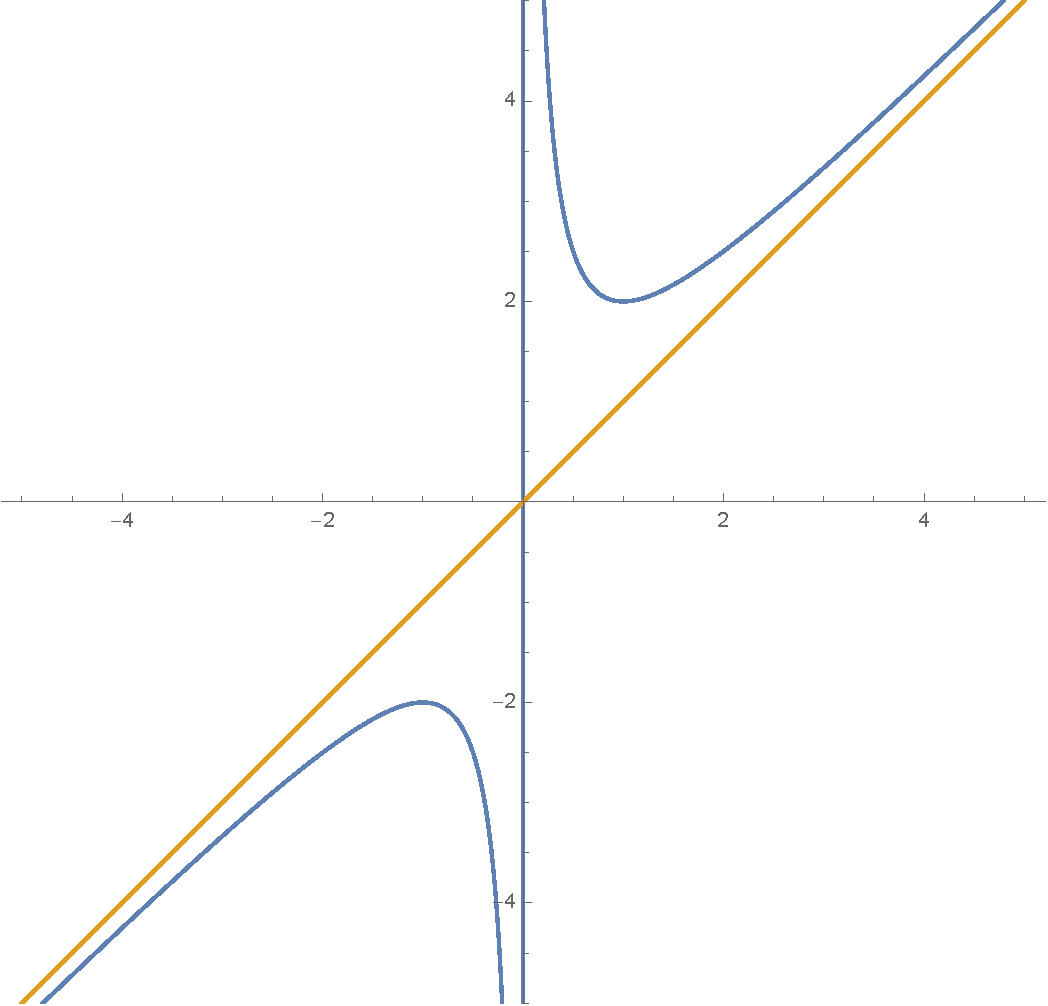
\includegraphics[width=7cm]{./images/ch3/x1x.pdf}
	\end{center}
\end{frame}

\begin{frame}
	\linespread{1.5}
	\ba{1.描绘下列函数的图形:(2)$y=e^{-(x-1)^2}$
	}
	
	\begin{center}
		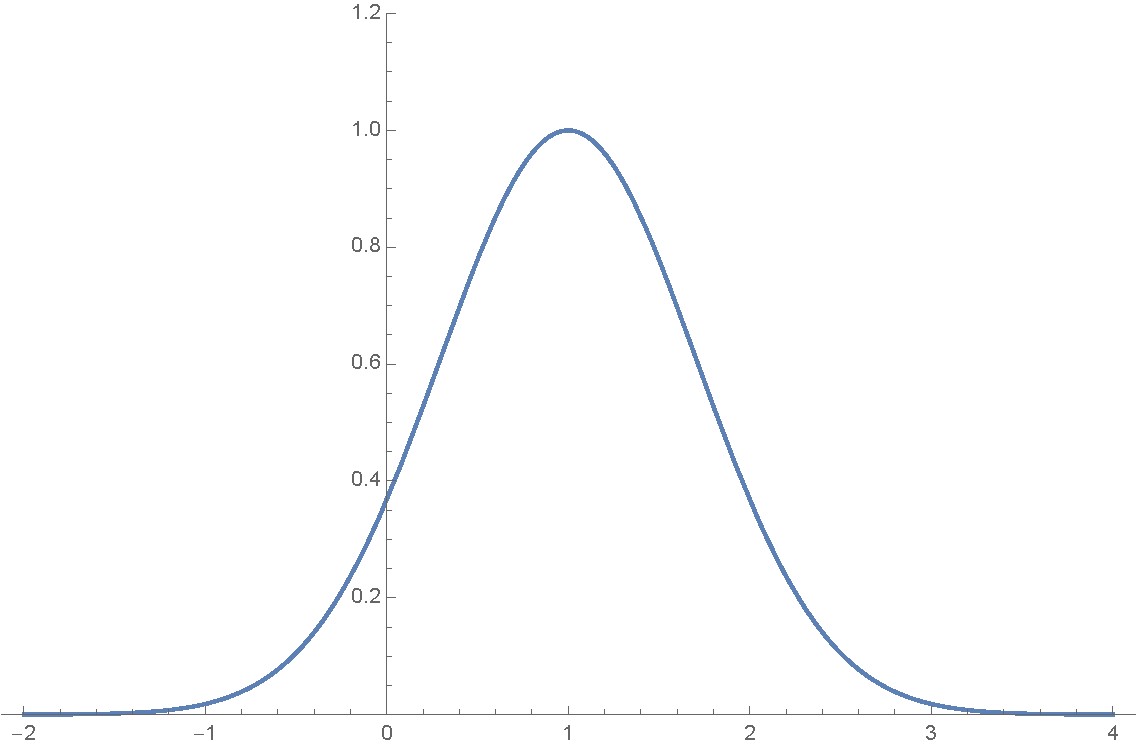
\includegraphics[width=8cm]{./images/ch3/e-2x.pdf}
	\end{center}
\end{frame}

% % !Mode:: "TeX:UTF-8"

\titlepage

% \begin{frame}{说在前面}
% 	\linespread{1.5}
% 	  \begin{itemize}[<+-|alert@+>]
% 	    \item 过往的作业不订正、不补齐的不予批改,打分不超过\,\ba{C}
% 	    \item 不交作业的默认记为\,\ba{D}
% 	    \item 需要换作业本的,请“移植”照片,写清楚个人信息
% 	    \item 请自行完成SPOC课程中的测试
% 	    \item 第二次单元测试即将发布,成绩记入期末总成绩
% 	  \end{itemize}
% \end{frame}

% \begin{frame}{需要注意的问题}
% 	\linespread{1.5}
% 	  \begin{itemize}%[<+-|alert@+>]
% 	    \item L'Hospital法则
% 	    \begin{itemize}
% 	      \item \it 只能应用于“$\df{\bm{0}}{\bm{0}}$”
% 	      和“$\df{\bm{\infty}}{\bm{\infty}}$”型
% 	      \item \it 及时使用无穷小代换进行简化
% 	      \item \it 不正规的符号:\b 
% 	      $\xlongequal{\footnotesize\mbox{“L”}}$、
% 	      $\xlongrightarrow{\footnotesize\mbox{“L'Hospital法则”}}$、
% 	      $\df{\bm{0}}{\bm{0}}$、$\df{\bm{\infty}}{\bm{\infty}}$
% 	    \end{itemize}
% 	    \item Taylor公式
% 	    \begin{itemize}
% 	      \item \it Taylor多项式不包含余项
% 	      \item \it 合并同次幂的系数
% 	      \item \it 尽量按照幂次由低到高排列,最后写余项
% 	    \end{itemize}
% 	  \end{itemize}
% \end{frame}

\begin{frame}{出现的问题}
	\linespread{1.5}
	{\bf 错在哪里?}
	
	\it\b
	由定积分中值定理,存在$\xi\in[a,b]$,使得
	\begin{align*}
		&\dint_a^bf(x)g(x)\d x=f(\xi)g(\xi)(b-a),\\
		&\dint_a^bg(x)\d x=g(\xi)(b-a),
	\end{align*}
	进而可得
	$$\dint_a^bf(x)g(x)\d x=f(\xi)\dint_a^bg(x)\d x.$$
\end{frame}

\begin{frame}{出现的问题}
	\linespread{1.5}
	{\bf 错在哪里?}
	
	\it\b
	由Lagrange中值定理,存在$\xi\in[a,b]$,使得
	\begin{align*}
		&f(b)-f(a)=f'(\xi)(b-a),\\
		&g(b)-g(a)=g'(\xi)(b-a),
	\end{align*}
	进而可得
	$$\df{f(b)-f(a)}{g(b)-g(a)}=\df{f'(\xi)}{g'(\xi)}.$$
\end{frame}

\section{5.1 定积分的概念与性质}

\begin{frame}
	\linespread{1.5}
	\ba{1.$f(x)$在$[a,b]$上非负,$x\in(a,b)$时$f''(x)>0$,$f'(x)<0$,
	$I_1=\frac{b-a}2[f(b)+f(a)]$,$I_2=\dint_a^bf(x)\d x$,$I_3=(b-a)f(b)$,
	试比较$I_1,I_2,I_3$的大小。}
	\pause
	
% 	\bigskip
	
	\small 解:\it
	$f'(x)<0$,故对任意$x\in(a,b)$,均有$f(a)>f(x)>f(b)$,从而
	$$(b-a)f(a)>\dint_a^bf(x)\d x>(b-a)f(b),$$
	由此可知$I_2>I_3$。
	\pause
	
	令$L(x)=f(a)+\df{f(b)-f(a)}{b-a}(x-a)$,
	由$f''(x)>0$,可知对任意$x\in(a,b)$,均有$f(x)<L(x)$,进而
	由定积分的保号性,可得
	$$\dint_a^bf(x)\d x<\dint_a^bL(x)\d x=\df{b-a}2[f(b)+f(a)],$$
	由此可得$I_2<I_1$。
	
	综上,$I_1>I_2>I_3$。\hfill$\Box$
\end{frame}

\begin{frame}
	\linespread{1.5}
	\ba{3.设$f(x)\in C[a,b]$,$g(x)>0$,证明:存在$\xi\in[a,b]$,使得
	$$\dint_a^bf(x)g(x)\d x=f(\xi)\dint_a^bg(x)\d x.$$}
	\pause
	
% 	\bigskip
	
	\small 证:\it 记$c=\frac{\int_a^bf(x)g(x)\d x}{\int_a^bg(x)\d x}$。
	由$f(x)\in C[a,b]$,可设$m,M$分别为$f(x)$在$[a,b]$上的
	最小和最大值,进而可知
	$$m\dint_a^bg(x)\d x\leq \dint_a^bf(x)g(x)\d x\leq M\dint_a^bg(x)\d x,$$
	从而	$m\leq c\leq M,$
	从而由连续函数的介值定理可知,必存在$\xi\in[a,b]$,使得
	$f(\xi)=c$,
	即证。\hfill$\Box$
\end{frame}

\begin{frame}
	\linespread{1.5}
	\ba{4.已知$f(x)$在$[0,\pi]$上连续,$(0,\pi)$内可导,且$f(0)=
	\dint_0^{\pi}f(x)\sin x\d x=0$,证明:存在$\xi\in(0,\pi)$,
	使得$f'(\xi)=0$。
	}\pause
	
	\bigskip
	
	\small 证:\it 
	$\dint_0^{\pi}f(x)\sin x\d x=0$,由定积分中值定理,可知必存在$\eta\in(0,\pi)$,
	使得$f(\eta)\sin\eta=0$。注意到$x\in(0,\pi)$时,$\sin x>0$,故必有
	$f(\eta)=0$。\pause
	
	至此,可以验证$f(x)$在$[0,\eta]$上满足Rolle定理条件,
	进而可知必存在$\xi\in(0,\eta)\subset (0,\pi)$,使得$f'(\xi)=0$。
	\hfill$\Box$
\end{frame}

\begin{frame}
	\linespread{1.5}
	\ba{5.设$f(x)$在$[0,1]$上连续,在$(0,1)$内可导,且$f(0)\cdot f(1)>0$,
	$f(1)+\dint_0^1f(x)\d x=0$,证明:存在$\xi\in(0,1)$,使得
	$f'(\xi)=\xi f(\xi)$。
	}\pause
	
	\bigskip
	
	\small 证:\it 
	不妨设$f(1)>0$,则$\dint_0^1f(x)\d x<0$,从而可知,存在$\eta_1\in(0,1)$,
	使得$f(\eta_1)<0$。进而由连续函数的介值定理,可知存在$\eta\in(0,\eta_1)$,
	使得$f(\eta)=0$。
	
	令$F(x)=e^{-\frac{x^2}2}f(x)$,可以验证$F(x)$在$[0,\eta]$上满足
	Rolle定理条件,从而可知必存在$\xi\in(0,\eta)\subset(0,1)$,使得
	$$F'(\xi)=e^{-\frac{\xi^2}2}[f'(\xi)-\xi f(\xi)]=0,$$
	因为$e^{-\frac{\xi^2}2}\ne0$,故必有$f'(\xi)-\xi f(\xi)=0$,即证。
	\hfill$\Box$
\end{frame}

\section{5.2 微积分基本公式}

\begin{frame}
	\linespread{1.5}
	\ba{1.计算下列定积分:
	(1)$\dint_{-1}^2[x]\max\{1,e^{-x}\}\d x$
	}
	
	\pause
	\small 解:\it 
	$$
		\dint_{-1}^2[x]\max\{1,e^{-x}\}\d x
		=-\dint_{-1}^0e^{-x}\d x+\dint_1^2\d x
		=2-e
	$$
\end{frame}

\begin{frame}
	\linespread{1.5}
	\ba{3.计算下列函数的导函数
	(1)$f(x)=\dint_0^xtg(x^2-t^2)\d t$,其中$g(x)$为连续函数;
	}
	
	\pause
	\small 解:\it 
	令$u=x^2-t^2$,则
	\begin{align*}
		f(x)&=\df12\dint_0^xg(x^2-t^2)\d t^2\\
		&=\df12\dint_{x^2}^0g(u)\d(x^2-u)
		=\df12\dint_0^{x^2}g(u)\d u,
	\end{align*}
	于是
	$$f'(x)=\df12g(x^2)2x=xg(x^2).$$
\end{frame}

\begin{frame}
	\linespread{1.5}
	\ba{3.计算下列函数的导函数
	(2)$f(x)=\dint_0^x\sin(x-t)^2\d t$。
	}
	
	\pause
	\small 解:\it 
	令$u=x-t$,则
	$$f(x)=\dint_x^0\sin u^2\d(x-u)=\dint_0^x\sin u^2\d u,$$
	故
	$$f'(x)=\sin x^2.$$
	\hfill$\Box$
\end{frame}

\begin{frame}
	\linespread{1.5}
	\ba{4.设曲线$y=f(x)$与$y=\dint_0^{\arctan x}e^{-t^2}\d t$在原点处
	相切,求$\limn nf\left(\df2n\right)$。
	}
	
	\pause
% 	\vspace{-1em}
	\small 解:\it 
	\begin{align*}
		\limn nf\left(\df2n\right)
		&=2\limn\df{f\left(\df2n\right)}{\df2n}
		=2\limx0\df{f(x)}x\\
		&=2\limx0f'(x)=2f'(0)=2y'(0)\\
		&=2e^{-\arctan^2 x}\left.\df1{1+x^2}\right|_{x=0}=2.
	\end{align*}
	\hfill$\Box$
\end{frame}

\begin{frame}
	\linespread{1.5}
	\ba{6.计算如下极限:
	(3)$\limx{+\infty}\df{\dint_0^x(\arctan t)^2\d t}{\sqrt{x^2+1}}$
	}
	
	\pause
% 	\vspace{-1em}
	\small 解:\it 
	$$
	\mbox{原式}=\limx{+\infty}\df{\dint_0^x(\arctan t)^2\d t}{x}
	=\limx{+\infty}(\arctan x)^2=\df{\pi^2}4.
	$$
	\hfill$\Box$
\end{frame}

% % !Mode:: "TeX:UTF-8"

\titlepage

% \begin{frame}{说在前面}
% 	\linespread{1.5}
% 	  \begin{itemize}[<+-|alert@+>]
% 	    \item 过往的作业不订正、不补齐的不予批改,打分不超过\,\ba{C}
% 	    \item 不交作业的默认记为\,\ba{D}
% 	    \item 需要换作业本的,请“移植”照片,写清楚个人信息
% 	    \item 请自行完成SPOC课程中的测试
% 	    \item 第二次单元测试即将发布,成绩记入期末总成绩
% 	  \end{itemize}
% \end{frame}

% \begin{frame}{需要注意的问题}
% 	\linespread{1.5}
% 	  \begin{itemize}%[<+-|alert@+>]
% 	    \item L'Hospital法则
% 	    \begin{itemize}
% 	      \item \it 只能应用于“$\df{\bm{0}}{\bm{0}}$”
% 	      和“$\df{\bm{\infty}}{\bm{\infty}}$”型
% 	      \item \it 及时使用无穷小代换进行简化
% 	      \item \it 不正规的符号:\b 
% 	      $\xlongequal{\footnotesize\mbox{“L”}}$、
% 	      $\xlongrightarrow{\footnotesize\mbox{“L'Hospital法则”}}$、
% 	      $\df{\bm{0}}{\bm{0}}$、$\df{\bm{\infty}}{\bm{\infty}}$
% 	    \end{itemize}
% 	    \item Taylor公式
% 	    \begin{itemize}
% 	      \item \it Taylor多项式不包含余项
% 	      \item \it 合并同次幂的系数
% 	      \item \it 尽量按照幂次由低到高排列,最后写余项
% 	    \end{itemize}
% 	  \end{itemize}
% \end{frame}

\begin{frame}{出现的问题}
	\linespread{1.5}
	  \begin{itemize}%[<+-|alert@+>]
	    \item 反常积分的审敛
	    \begin{itemize}
	      \item \it\b 函数$f(x)$在$[1,+\infty)$上有界,故
	      $\dint_1^{+\infty}f(x)\d x$收敛;
	      \item \it\b 函数$f(x)$在$(0,1)$上无界,故
	      $\dint_0^1f(x)\d x$发散;
	      \item \it\b $\limx{+\infty}\df{\cos x}{\ln x}=0$,故由无穷积分收敛
	      的必要条件,积分$\dint_2^{+\infty}\df{\cos x}{\ln x}\d x$收敛;
	      \item \it\b $\limx{1^+}\df{(x-1)\cos x}{\ln x}=1$,故由极限审敛法2,
	      积分$\dint_2^{+\infty}\df{\cos x}{\ln x}\d x$发散。   
	    \end{itemize}
	  \end{itemize}
\end{frame}

\section{5.3 定积分的计算-换元法和分部积分法}

\begin{frame}
	\linespread{1.5}
	\ba{1.计算下列定积分:(1)$\dint_0^4e^{\sqrt x}\d x$}
	\pause
	
% 	\bigskip
	
	\small 解:\it
	$$\mbox{原式}\xlongequal{t=\sqrt x}
	\dint_0^2e^t2t\d t=2te^t|_0^2-2\dint_0^2e^t\d t
	=2e^2+2.$$
\end{frame}

\begin{frame}
	\linespread{1.5}
	\ba{1.计算下列定积分:
	(2)$\dint_{-\frac{\pi}2}^{\frac{\pi}2}(x^3+\sin^2x)\cos^2x\d x$}
	\pause
	
% 	\bigskip
	
	\small 解:\it
	由对称区间上定积分的性质,
	$\dint_{-\frac{\pi}2}^{\frac{\pi}2}x^3\cos^2x\d x=0$,
	又注意到$\dint_{-\frac{\pi}2}^{\frac{\pi}2}\cos4x\d x=0$
	故
	\begin{align*}
		\mbox{原式}
		&=\dint_{-\frac{\pi}2}^{\frac{\pi}2}\sin^2x\cos^2x\d x
		=\df14\dint_{-\frac{\pi}2}^{\frac{\pi}2}\sin^22x\d x\\
		&=\df12\dint_{0}^{\frac{\pi}2}\df{1-\cos 4x}2\d x
		=\df{\pi}{8}.
	\end{align*}
\end{frame}

\begin{frame}
	\linespread{1.5}
	\ba{1.计算下列定积分:
	(3)$\dint_0^{\frac{3\pi}4}\df{\d x}{1+\sin^2x}$}
	\pause
	
% 	\bigskip
	
	\small 解:\it
	\begin{align*}
		\mbox{原式}&=\dint_0^{\frac{3\pi}4}\df{\csc^2x\d x}{\csc^2x+1}
		=-\dint_0^{\frac{3\pi}4}\df{\d\cot x}{\cot^2x+2}\\
		&=-\df1{\sqrt2}\dint_0^{\frac{3\pi}4}\df{\d\frac{\cot x}{\sqrt2}}
		{\left(\frac{\cot x}{\sqrt2}\right)^2+1}
		=-\left.\df1{\sqrt2}\arctan\df{\cot x}{\sqrt2}\right|_0^{\frac{3\pi}4}\\
		&=\df1{\sqrt2}\arctan\df1{\sqrt2}
		=\df1{\sqrt2}\left(\pi-\arctan\sqrt2\right).
	\end{align*}
\end{frame}

\begin{frame}
	\linespread{1.5}
	\ba{1.计算下列定积分:
	(4)$\dint_0^{\frac{\pi}2}\df{\d x}{1+(\tan x)^{\sqrt 2}}$}
	\pause
	
% 	\bigskip
	
	\small 解:\it
	由对称性
	\begin{align*}
		\mbox{原式}&=\dint_0^{\frac{\pi}2}\df{(\cos x)^{\sqrt 2}\d x}
		{(\cos x)^{\sqrt 2}+(\sin x)^{\sqrt 2}}
		=\dint_0^{\frac{\pi}2}\df{(\sin x)^{\sqrt 2}\d x}
		{(\cos x)^{\sqrt 2}+(\sin x)^{\sqrt 2}}\\
		&=\df12\dint_0^{\frac{\pi}2}\df{(\cos x)^{\sqrt 2}+(\sin x)^{\sqrt 2}}
		{(\cos x)^{\sqrt 2}+(\sin x)^{\sqrt 2}}\d x
		=\df12\dint_0^{\frac{\pi}2}\d x=\df{\pi}4.
	\end{align*}
	
	\ba{注:$\dint_0^af(x)\d x=\dint_0^af(a-x)\d x$}
\end{frame}

\begin{frame}
	\linespread{1.5}
	\ba{1.计算下列定积分:
	(5)$\dint_{\frac12}^{\frac32}\df{(1-x)\arcsin(1-x)}{\sqrt{2x-x^2}}\d x$}
	\pause
	
% 	\bigskip
	
	\small 解:\it
	注意到
	$$\dint_{\frac12}^1\df{(1-x)\arcsin(1-x)}{\sqrt{2x-x^2}}\d x
	\xlongequal{y=2-x}\dint_1^{\frac32}\df{(1-y)\arcsin(1-y)}
	{\sqrt{2y-y^2}}\d y,$$
	故
	\begin{align*}
		\mbox{原式}
		&=2\dint_{\frac12}^1\df{(1-x)\arcsin(1-x)}{\sqrt{2x-x^2}}\d x
		=2\dint_{\frac12}^1\df{(1-x)\arcsin(1-x)}{\sqrt{1-(1-x)^2}}\d x\\
		&\xlongequal{t=1-x}2\dint_0^{\frac12}\df{t\arcsin t}{\sqrt{1-t^2}}\d t
		=-2\dint_0^{\frac12}\arcsin t\d{\sqrt{1-t^2}}\\
		&=-2\left.\sqrt{1-t^2}\arcsin t\right|_0^{\frac12}
		+2\dint_0^{\frac12}\d t
		=-\df{\sqrt3\pi}6+1.
	\end{align*}
\end{frame}

\begin{frame}
	\linespread{1.5}
	\ba{1.计算下列定积分:
	(6)$\dint_{-\frac{\pi}4}^{\frac{\pi}4}e^{\frac x2}
	\df{\cos x-\sin x}{\sqrt{\cos x}}\d x$}
	\pause
	
% 	\bigskip
	
	\small 解:\it
	\begin{align*}
		\mbox{原式}
		&=\dint_{-\frac{\pi}4}^{\frac{\pi}4}e^{\frac x2}\sqrt{\cos x}\d x
		+2\dint_{-\frac{\pi}4}^{\frac{\pi}4}e^{\frac x2}\d\sqrt{\cos x}\\
		&=\dint_{-\frac{\pi}4}^{\frac{\pi}4}e^{\frac x2}\sqrt{\cos x}\d x
		+2\left.e^{\frac x2}\sqrt{\cos x}\right|_{-\frac{\pi}4}^{\frac{\pi}4}
		-\dint_{-\frac{\pi}4}^{\frac{\pi}4}e^{\frac x2}\sqrt{\cos x}\d x\\
		&=\sqrt[4]8\left(e^{\frac{\pi}8}-e^{-\frac{\pi}8}\right).
	\end{align*}
\end{frame}

\begin{frame}
	\linespread{1.5}
	\ba{1.计算下列定积分:
	(7)$\dint_{-2}^2\df{x+\sin x+|x|}{2+x^2}\d x$}
	\pause
	
% 	\bigskip
	
	\small 解:\it
	\begin{align*}
		\mbox{原式}
		&=\dint_{-2}^2\df{|x|}{2+x^2}\d x
		=2\dint_0^2\df{x}{2+x^2}\d x\\
		&=\dint_0^2\df{\d x^2}{2+x^2}
		=\left.\ln(2+x^2)\right|_0^2=\ln3.
	\end{align*}
\end{frame}

\begin{frame}
	\linespread{1.5}
	\ba{1.计算下列定积分:
	(8)$\dint_{\frac12}^{\frac32}\df{\d x}{\sqrt{|x^2-x|}}$}
	\pause
	
% 	\bigskip
	
	\small 解:\it
	\begin{align*}
		\mbox{原式}
		&=\dint_{\frac12}^1\df{\d x}{\sqrt{x(1-x)}}
		+\dint_1^{\frac32}\df{\d x}{\sqrt{x(x-1)}}\\
		&=2\dint_{\frac12}^1\df{\d\sqrt x}{\sqrt{1-(\sqrt x)^2}}
		+2\dint_1^{\frac32}\df{\d\sqrt x}{\sqrt{(\sqrt x)^2-1}}\\
		&=2\left.\arcsin\sqrt x\right|_{\frac12}^1
		+2\dint_0^{\arccos\sqrt{\frac23}}\df{\d\sec t}{\sqrt{\sec^2t-1}}\\
		&=\df{\pi}2+2\dint_0^{\arccos\sqrt{\frac23}}\sec t\d t\\
		&=\df{\pi}2+2\ln\left|\sec t+\tan t\right|_0^{\arccos\sqrt{\frac23}}
		=\df{\pi}2+\ln(2+\sqrt3).
	\end{align*}
	\hfill$\Box$
\end{frame}

\begin{frame}
	\linespread{1.5}
	\ba{2.设$f(x),g(x)$在$[0,1]$上导函数连续,且$f(0)=0$,$f'(x)\geq0$,
	$g'(x)\geq0$,证明:对任意$a\in[0,1]$,总有
	$$\dint_0^ag(x)f'(x)\d x+\dint_0^1f(x)g'(x)\d x\geq f(a)g(1).$$
	}
	
	\pause
% 	\vspace{-1em}
	\small 证:\it 
	由$f(0)=0$,
	\begin{align*}
		&\dint_0^1f(x)g'(x)\d x=\dint_0^1f(x)\d g(x)\\
		&=\left.f(x)g(x)\right|_0^1-\dint_0^1g(x)\d f(x)
		=f(1)g(1)-\dint_0^1g(x)f'(x)\d x.
	\end{align*}
	故待证不等式左端即为$f(1)g(1)+\dint_1^ag(x)f'(x)\d x$.
\end{frame}

\begin{frame}
	\linespread{1.5}
	\ba{2.设$f(x),g(x)$在$[0,1]$上导函数连续,且$f(0)=0$,$f'(x)\geq0$,
	$g'(x)\geq0$,证明:对任意$a\in[0,1]$,总有
	$$\dint_0^ag(x)f'(x)\d x+\dint_0^1f(x)g'(x)\d x\geq f(a)g(1).$$
	}
	
	\pause
% 	\vspace{-1em}
	\small 续:\it 
	\ldots,	故待证不等式左端即为$f(1)g(1)+\dint_1^ag(x)f'(x)\d x$,令
	$$F(a)=\dint_1^ag(x)f'(x)\d x+f(1)g(1)-f(a)g(1),$$
	则$F'(a)=f'(a)[g(a)-g(1)]$。已知$g'(x)\geq0$,故
	$g(a)-g(1)\leq 0$,又$f'(x)\geq0$,故$F'(a)\leq0$,
	也即$F(a)$在$[0,1]$上单调递减。注意到$F(1)=0$,从而可知
	$F(a)\geq 0$,即证。
	\hfill$\Box$
\end{frame}

\begin{frame}
	\linespread{1.5}
	\ba{\small 3.设$f(x),g(x)$在$[a,b]$上连续,且满足$x\in[a,b)$时,
	$$\dint_a^xf(t)\d t>\dint_a^xg(t)\d t,\;
	\;\dint_a^bf(x)\d x=\dint_a^bg(x)\d x,$$
	证明:$\dint_a^bxf(x)\d x<\dint_a^bxg(x)\d x$。
	}
	
	\pause
% 	\vspace{-1em}
	\small 证:\it 
	记$H(x)=\dint_a^x[f(t)-g(t)]\d t$,则
	$H(x)\geq 0$,$H(b)=H(a)=0$,于是
	\begin{align*}
		&\dint_a^bx[f(x)-g(x)]\d x
		=\dint_a^bx\d H(x)\\
		&=\left.xH(x)\right|_a^b-\dint_a^bH(x)\d x
		=-\dint_a^bH(x)\d x\leq 0,
	\end{align*}
	即证。\hfill$\Box$
\end{frame}

\begin{frame}
	\linespread{1.5}
	\ba{4.设$f(x)\in C[a,b]$且严格单调递增,证明:
	$$(a+b)\dint_a^bf(x)\d x<2\dint_a^bxf(x)\d x.$$
	}
	
	\pause
% 	\vspace{-1em}
	\small 证一:\it 
	注意到
	$\dint_a^b\left(x-\df{a+b}2\right)f\left(\df{a+b}2\right)\d x=0$,
	故
	\begin{align*}
		\dint_a^b\left(x-\df{a+b}2\right)f(x)\d x
		&=\dint_a^b\left(x-\df{a+b}2\right)\left[f(x)
		-f\left(\df{a+b}2\right)\right]\d x,
	\end{align*}
	由于$f(x)$在$[a,b]$上严格单调递增,故对任意$x\in(a,b)$,均有
	$$\left(x-\df{a+b}2\right)\left[f(x)
	-f\left(\df{a+b}2\right)\right]>0,$$
	从而可知
	$\dint_a^b\left(x-\df{a+b}2\right)f(x)\d x>0,$
	即证。\hfill$\Box$
\end{frame}

\begin{frame}
	\linespread{1.5}
	\ba{4.设$f(x)\in C[a,b]$且严格单调递增,证明:
	$$(a+b)\dint_a^bf(x)\d x<2\dint_a^bxf(x)\d x.$$
	}
	
	\pause
% 	\vspace{-1em}
	\small 证二:\it 
	令
	$$F(x)=(a+x)\dint_a^xf(t)\d t-2\dint_a^xtf(t)\d t,$$
	则
	$$F'(x)=\dint_a^x[f(t)-f(x)]\d t,$$
	由于$f(x)$严格单调递增,故总有$f(t)-f(x)<0$,进而$F'(x)<0$,
	又$F(a)=0$,从而可知$F(b)<0$,即证。\hfill$\Box$
\end{frame}

\begin{frame}
	\linespread{2}
	\ba{5.设$f(x)$是以$T$为周期的连续函数
	  \begin{enumerate}[(1)]
% 	    \setlength{\itemindent}{1cm}
	    \item 证明:$\dint_0^xf(t)\d t$可以表示为一个以$T$
	    为周期的函数$g(x)$与$kx$之和,求此常数$k$;
	    \item 计算$\limx{\infty}\df1x\dint_0^xf(t)\d t$;
	    \item 设$[x]$为不超过$x$的最大整数,$g(x)=x-[x]$,计算
	    $\limx{\infty}\df1x\dint_0^xg(t)\d t$。
	  \end{enumerate}
	}
\end{frame}

\begin{frame}
	\linespread{1.5}
	\small 解:(1)\it 
	记$k=\df1T\dint_0^Tf(x)\d x$,令$g(x)=\dint_0^xf(t)\d t-kx$,
	则对任意$x$,有
	\begin{align*}
		g(x+T)
		&=\dint_0^{x+T}f(t)\d t-k(x+T)\\
		&=\dint_0^xf(t)\d t-kx+\dint_x^{x+T}f(t)\d t-kT\\
		&=g(x)+\dint_0^{T}f(t)\d t-kT=g(x),
	\end{align*}
	也即$g(x)$是以$T$为周期的函数,即证。
\end{frame}

\begin{frame}
	\linespread{1.5}
	\small 解:(2){\it 
	显然$g(x)$是一个连续的周期函数,故必有界,从而可知$\limx{\infty}\df{g(x)}x=0$,
	于是}
	$$\limx{\infty}\df1x\dint_0^xf(t)\d t=\limx{\infty}\df{g(x)+kx}x=k
	=\df1T\dint_0^Tf(x)\d x.$$
	
	(3)\it $g(x)$是以$1$为周期的函数,且$\dint_0^1(x-[x])\d x=\df12$,故由(2)的结论,
	可知$\limx{\infty}\df1x\dint_0^xg(t)\d t=\df12$。
	\hfill$\Box$
\end{frame}

\section{5.4 反常积分}

\begin{frame}
	\linespread{1.5}
	\ba{1.计算下列积分:
	(1)$\dint_1^{+\infty}\df{\arctan x}{x^2}\d x$
	}
	
	\pause
% 	\vspace{-1em}
	\small 解:\it 
	\begin{align*}
		\mbox{原式}
		&=-\dint_1^{+\infty}\arctan x\d\df1x
		=-\left.\df{\arctan x}x\right|_1^{+\infty}
		+\dint_1^{+\infty}\df1x\d\arctan x\\
		&=\df{\pi}4+\dint_1^{+\infty}\df1{x(1+x^2)}\d x
		=\df{\pi}4+\df12\dint_1^{+\infty}\left(\df1{x^2}-\df1{1+x^2}\right)\d x^2\\
		&=\df{\pi}4+\left.\df12\left[\ln x^2-\ln(1+x^2)\right]\right|_1^{+\infty}
		=\df{\pi}4+\df12\ln2.
	\end{align*}
\end{frame}

\begin{frame}
	\linespread{1.5}
	\ba{1.计算下列积分:
	(2)$\dint_2^{+\infty}\df{\d x}{(x+7)\sqrt{x-2}}$
	}
	
	\pause
% 	\vspace{-1em}
	\small 解:\it 
	\begin{align*}
		\mbox{原式}
		&=\dint_2^{+\infty}\df{\d\sqrt{x-2}}{(\sqrt{x-2})^2+9}
		\xlongequal{u=\sqrt{x-2}}2\dint_0^{+\infty}\df{\d u}{u^2+9}\\
		&=\left.\df23\arctan\df u3\right|_0^{+\infty}=\df{\pi}3.
	\end{align*}
\end{frame}

\begin{frame}
	\linespread{1.5}
	\ba{1.计算下列积分:
	(3)$\dint_1^{+\infty}\df{\d x}{x\sqrt{1+2x^4+2x^8}}$
	}
	
	\pause
% 	\vspace{-1em}
	\small 解:\it 
	\begin{align*}
		\mbox{原式}
		&=\df14\dint_1^{+\infty}\df{\d x^4}{x^4\sqrt{1+2x^4+2x^8}}
		\xlongequal{u=x^4}\df1{4\sqrt2}\dint_1^{+\infty}\df{\d u}
		{u\sqrt{\left(u+\frac12\right)^2+\frac14}}\\
		&\xlongequal{u=\frac12(\tan t-1)}\df1{2\sqrt2}
		\dint_{\arctan3}^{\frac{\pi}2}\df{\d t}{\sin t-\cos t}
		=\df14\dint_{\arctan3}^{\frac{\pi}2}\df{\d t}
		{\sin\left(t-\frac{\pi}4\right)}\\
		&\xlongequal{y=t-\frac{\pi}4}\df14
		\dint_{\arctan3-\frac{\pi}4}^{\frac{\pi}4}\csc y\d y
		=\df14\dint_{\arctan3-\frac{\pi}4}^{\frac{\pi}4}
		\df{\csc y(\csc y+\cot y)}{\csc y+\cot y}\d y\\
		&=-\left.\df14\ln|\csc y+\cot y|\right|
		_{\arctan3-\frac{\pi}4}^{\frac{\pi}4}
		=\df14\ln\df{2+\sqrt 5}{1+\sqrt 2}.
	\end{align*}
\end{frame}

\begin{frame}
	\linespread{1.5}
	\ba{1.计算下列积分:
	(4)$\dint_{-1}^0\df{\ln(1+x)}{\sqrt[3]{1+x}}\d x$
	}
	
	\pause
% 	\vspace{-1em}
	\small 解:\it 
	\begin{align*}
		\mbox{原式}
		&\xlongequal{y=\sqrt[3]{1+x}}9\dint_0^1u\ln u\d u
		=\df92\dint_0^1\ln u\d u^2\\
		&=\left.\df92u^2\ln u\right|_0^1-\df92\dint_0^1u\d u\\
		&=-\df92\lim\limits_{u\to0^+}u^2\ln u-\df94=-\df94.
	\end{align*}
\end{frame}

\begin{frame}
	\linespread{1.5}
	\ba{1.计算下列积分:
	(5)$\dint_0^{+\infty}\df{\d x}{e^{x+1}+e^{1-x}}$
	}
	
	\pause
% 	\vspace{-1em}
	\small 解:\it 
	$$
		\mbox{原式}
		=\df1e\dint_0^{+\infty}\df{e^x\d x}{e^{2x}+1}
		=\left.\df1e\arctan e^x\right|_0^{+\infty}=\df{\pi}{4e}.
	$$
	\hfill$\Box$
\end{frame}

\begin{frame}
	\linespread{1.5}
	\ba{2.已知$\dint_0^{+\infty}\df{\sin x}x\d x=\df{\pi}2$,求
	$\dint_0^{+\infty}\df{\sin^2x}{x^2}\d x$。
	}
	
	\pause
% 	\vspace{-1em}
	\small 解:\it 
	\begin{align*}
		&\dint_0^{+\infty}\df{\sin^2x}{x^2}\d x
		=-\dint_0^{+\infty}\sin^2x\d\df1x\\
		&=-\left.\df{\sin^2x}x\right|_0^{+\infty}
		+\dint_0^{+\infty}\df1x\d\sin^2x\\
		&=\dint_0^{+\infty}\df{2\sin x\cos x}x\d x
		=\dint_0^{+\infty}\df{\sin2x}{2x}\d 2x\\
		&=\dint_0^{+\infty}\df{\sin u}{u}\d u=\df{\pi}2.
	\end{align*}
	\hfill$\Box$
\end{frame}

\section{5.5 反常积分的审敛法与$\Gamma$函数}

\begin{frame}
	\linespread{1.5}
	\ba{1. 判定如下反常积分的敛散性:
	
	(1)$\dint_1^{+\infty}\df{x^2\d x}{(x+1)\sqrt[2]{x^3+1}}$
	}
	
	\pause
% 	\vspace{-1em}
	\small 解:\it 
	注意到
	$$\limx{+\infty}x^{\frac12}\df{x^2}{(x+1)\sqrt[2]{x^3+1}}=1,$$
	而$\dint_1^{+\infty}\df{\d x}{x^{\frac12}}$发散,故由比较判别法,
	该无穷积分发散。
\end{frame}

\begin{frame}
	\linespread{1.5}
	\ba{1. 判定如下反常积分的敛散性:	(2)$\dint_1^2\df{\d x}{(\ln x)^4}$
	}
	
	\pause
% 	\vspace{-1em}
	\small 解:\it 
	令$x=e^t$,原积分可化为
	$$\dint_0^{\ln 2}\df{e^t\d t}{t^4},$$
	注意到
	$$\limx{0^+}x^4\df{e^x}{x^4}=1,$$
	而瑕积分$\dint_0^{\ln 2}\df{\d x}{x^4}$发散,故由比较判别法,
	该瑕积分发散。
\end{frame}

\begin{frame}
	\linespread{1.5}
	\ba{1. 判定如下反常积分的敛散性:	
	(3)$\dint_1^{+\infty}\sin\df1{x^2}\d x$
	}
	
	\pause
% 	\vspace{-1em}
	\small 解:\it 
	注意到
	$$\limx{+\infty}x^2\sin\df1{x^2}=1,$$
	而无穷积分$\dint_1^{+\infty}\df{\d x}{x^2}$收敛,故由比较判别法,
	该无穷积分收敛。
\end{frame}

\begin{frame}
	\linespread{1.5}
	\ba{1. 判定如下反常积分的敛散性:	
	(4)$\dint_1^2\df{\d x}{\sqrt{3x-x^2-2}}$
	}
	
	\pause
% 	\vspace{-1em}
	\small 解:\it 
	注意到$\limx{1^+}\sqrt{x-1}\df1{\sqrt{x^2-3x+2}}
	=\limx{2^-}\sqrt{x-2}\df1{\sqrt{x^2-3x+2}}=1$,且
	$\dint_1^{\frac32}\df{\d x}{\sqrt{x-1}}$和$\dint_{\frac32}^2\df{\d
	x}{\sqrt{2-x}}$ 均收敛,故由比较判别法,
	积分$\dint_1^{\frac32}\df{\d x}{\sqrt{3x-x^2-2}}$和
	$\dint_{\frac32}^2\df{\d x}{\sqrt{3x-x^2-2}}$均收敛,进而
	原瑕积分收敛。
\end{frame}

\begin{frame}
	\linespread{1.5}
	\ba{1. 判定如下反常积分的敛散性:	
	(5)$\dint_2^{+\infty}\df{\cos x}{\ln x}\d x$
	}
	
	\pause
% 	\vspace{-1em}
	\small 解:\it 
	$$
		\dint_2^{+\infty}\df{\cos x}{\ln x}\d x=\ldots
		=-\df{\sin2}{\ln2}-\df{\cos2}{2\ln^2x}
		+\dint_2^{+\infty}\df{\ln x+2}{x^2\ln^3x}\cos x\d x.
	$$
	注意到
	$$\limx{+\infty}x^2\left|\df{\ln x+2}{x^2\ln^3x}\cos x\right|=0,$$
	注意到无穷积分$\dint_2^{+\infty}\df{\d x}{x^2}$收敛,故由比较判别法,
	无穷积分$\dint_2^{+\infty}\df{\ln x+2}{x^2\ln^3x}\cos x\d x$绝对收敛,
	从而收敛,于是可知原积分收敛。\hfill$\Box$
\end{frame}

\begin{frame}
	\linespread{1.5}
	\ba{2.设反常积分$\dint_1^{+\infty}f^2(x)\d x$收敛,证明反常积分
	$\dint_1^{+\infty}\df{f(x)}x\d x$绝对收敛。
	}
	
	\pause
% 	\vspace{-1em}
	\small 证:\it 
	由平均值不等式,$x\geq 1$时,
	$$\df{|f(x)|}x\leq\df12\left[f^2(x)+\df1{x^2}\right],$$
	从而
	$$\dint_1^{+\infty}\df{|f(x)|}x\d x
	\leq\df12\dint_1^{+\infty}\left[f^2(x)+\df1{x^2}\right]\d x,$$
	注意到积分$\dint_1^{+\infty}f^2(x)\d x$和$\dint_1^{+\infty}\df1{x^2}\d x$
	均收敛,故由比较判别法,积分$\dint_1^{+\infty}\df{|f(x)|}x\d x$收敛,
	也即$\dint_1^{+\infty}\df{f(x)}x\d x$绝对收敛。\hfill$\Box$
\end{frame}

\begin{frame}
	\linespread{1.5}
	\ba{3.利用$\Gamma$函数的性质证明Legendre倍量公式:
	$$\sqrt{\pi}\Gamma(2n)=2^{2n-1}\Gamma(n)\Gamma\left(n+\df12\right).$$
	}
	
	\pause
% 	\vspace{-1em}
	\small 证:\it 由$\Gamma(x+1)=x\Gamma(x)$,$\Gamma\left(\df12\right)=\sqrt{\pi}$,
	\begin{align*}
		\mbox{左边}&=(2n-1)!\sqrt{\pi},\\
		\mbox{右边}&=2^{2n-1}(n-1)!
		\df{2n-1}2\df{2n-3}2\ldots\df12\sqrt{\pi},\\
		&=(2n-2)!!(2n-1)!!\sqrt{\pi}=\mbox{左边}.
	\end{align*}
	即证。\hfill$\Box$
\end{frame}

% % !Mode:: "TeX:UTF-8"

\titlepage

\begin{frame}{说在前面}
	\linespread{1.5}
	  \begin{itemize}[<+-|alert@+>]
	    \item 如果对自己的作业成绩存在疑问,可以私信我查询本学期各次作业的成绩,
	    如果我的记录与实际情况不符,欢迎发难
	    \item 本子太烂了就换本新的吧
	    \item 本子还不算特别烂的下学期请继续使用
	    \item 新本子:贴照片,写上姓名、专业、学号、籍贯
	  \end{itemize}
\end{frame}

% \begin{frame}{需要注意的问题}
% 	\linespread{1.5}
% 	  \begin{itemize}%[<+-|alert@+>]
% 	    \item L'Hospital法则
% 	    \begin{itemize}
% 	      \item \it 只能应用于“$\df{\bm{0}}{\bm{0}}$”
% 	      和“$\df{\bm{\infty}}{\bm{\infty}}$”型
% 	      \item \it 及时使用无穷小代换进行简化
% 	      \item \it 不正规的符号:\b 
% 	      $\xlongequal{\footnotesize\mbox{“L”}}$、
% 	      $\xlongrightarrow{\footnotesize\mbox{“L'Hospital法则”}}$、
% 	      $\df{\bm{0}}{\bm{0}}$、$\df{\bm{\infty}}{\bm{\infty}}$
% 	    \end{itemize}
% 	    \item Taylor公式
% 	    \begin{itemize}
% 	      \item \it Taylor多项式不包含余项
% 	      \item \it 合并同次幂的系数
% 	      \item \it 尽量按照幂次由低到高排列,最后写余项
% 	    \end{itemize}
% 	  \end{itemize}
% \end{frame}

\begin{frame}{出现的问题}
	\linespread{1.5}
	  \begin{itemize}%[<+-|alert@+>]
	    \item 不画图!!!
	    \begin{itemize}
	      \item \b\it 不会画图
	      \item \b\it 不爱画图
	      \item \b\it 不想画图
	      \item \b\it 你懂的\ldots\ldots
	    \end{itemize}
	    \item 不交作业\ldots\ldots 不是问题:P
	  \end{itemize}
\end{frame}

\section{6.2 定积分的几何应用}

\begin{frame}
	\linespread{1.5}
	\ba{1. 设$S(t)$为直线$l_t:x+y=t(t\geq0)$下方位于正方形区域
	$D:0\leq x\leq 1,0\leq y\leq 1$内的\underline{面积},求$\dint_0^xS(t)\d t$。}
	\pause
	
% 	\bigskip
	
	\small 要点:\it
	$$S(t)=\left\{\begin{array}{ll}
		\df12t^2,& 0\leq t<1;\\ 1-\df12(2-t)^2, & 1\leq t <2;\\
		1,& t>2. 
	\end{array}\right.$$
	\ldots
	$$\dint_0^xS(t)\d t=\left\{\begin{array}{ll}
		\df16x^3,& 0\leq 0\leq x<1;\\ 
		\df16+(x-1)+\df16(2-x)^3, & 1<x\leq2;\\
		x-\df13,& x>2. 
	\end{array}\right.$$
\end{frame}

\begin{frame}
	\linespread{1.5}
	\ba{2.计算下列曲线的弧长:(1)$y=\ln(1-x^2)$,$0\leq x\leq\df12$}
	\pause
	
% 	\bigskip
	
	\small 解:\it
	弧长微元
	$$\alert{\d s=\sqrt{1+[y'(x)]^2}\d x}=\df{1+x^2}{1-x^2}\d
	x,\;(x\in\left[0,\df12\right]),$$
	故所求弧长
	$$s=\dint_0^{\frac12}\df{1+x^2}{1-x^2}\d x
	=\dint_0^{\frac12}\left[\df1{1+x}+\df1{1-x}-1\right]\d x
	=\ln3-\df12.$$
\end{frame}

\begin{frame}
	\linespread{1.5}
	\ba{2.计算下列曲线的弧长:
	(2)$\rho=a(1+\cos\theta)$,$0\leq\theta\leq2\pi$}
	\pause
	
% 	\bigskip
	
	\small 解:\it
	弧长微元
	$$\alert{\d s=\sqrt{\rho^2(\theta)+[\rho'(\theta)]^2}\d\theta}
	=2a\left|\cos\df{\theta}2\right|\d\theta,\;\theta\in[0,2\pi],$$
	故所求弧长
	$$s=\dint_0^{2\pi}2a\left|\cos\df{\theta}2\right|\d\theta
	=4a\dint_0^{\pi}\cos\df{\theta}2\d\theta
	=8a.$$
\end{frame}

\begin{frame}
	\linespread{1.5}
	\ba{3.设$D$是由曲线$y=\sin x+1$与三条直线$x=0,x=\pi,y=0$
	所围成的曲边梯形,求$D$绕$x$轴旋转一周所围成的旋转体的体积。
	}
	\pause
	
% 	\bigskip
	
	\begin{columns}
		\begin{column}{.5\textwidth}
			\begin{center}
				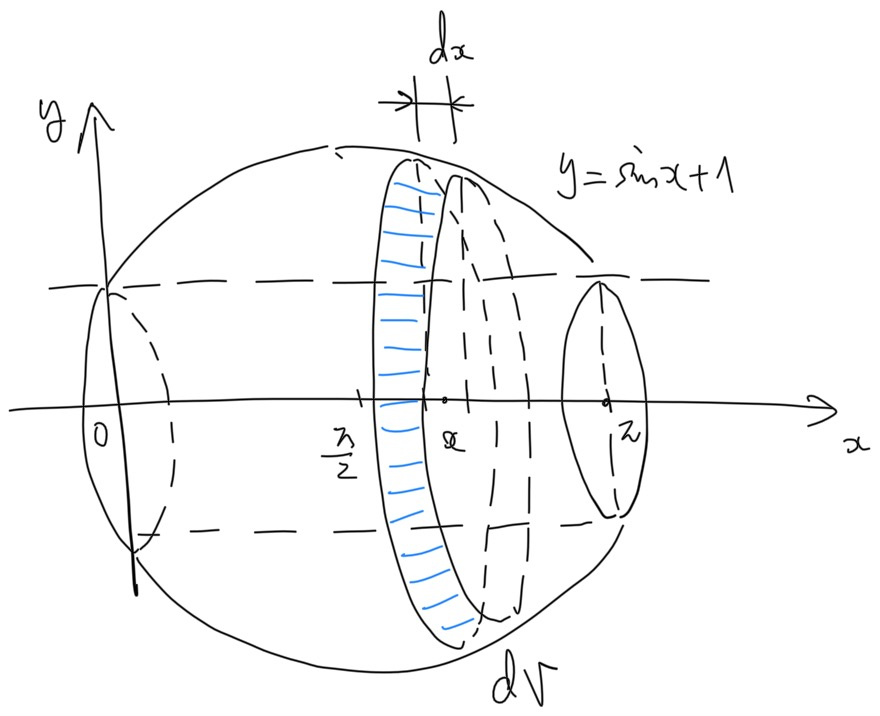
\includegraphics[width=.9\textwidth]{./images/ch6/sinx1cs.jpg}
		% 		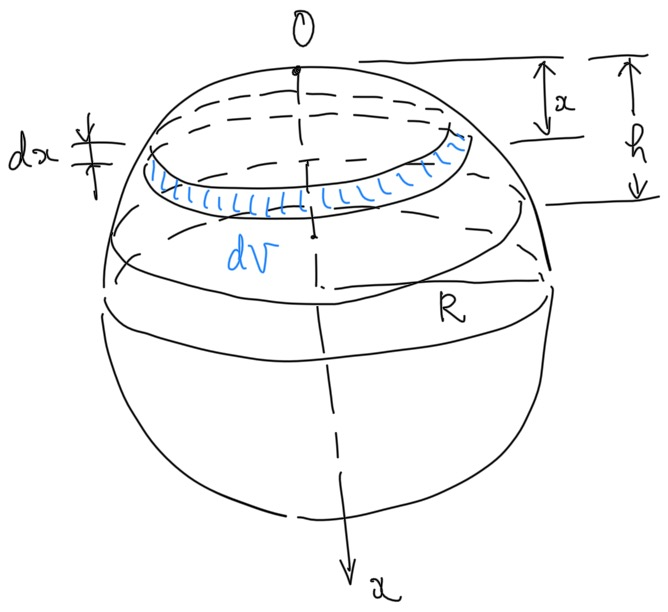
\includegraphics[width=6cm]{./images/ch6/topSp.jpg}
			\end{center}		
		\end{column}
		\begin{column}{.5\textwidth}
			\small 解:\it
			如图,体积微元$\d V=\pi y^2\d x$,	故所求体积
			$$
				V=\dint_0^{\pi}\pi(\sin x+1)^2\d x=\df32\pi^2.
			$$
		\end{column}
	\end{columns}
\end{frame}

\begin{frame}
	\linespread{1.5}
	\ba{4.证明球冠(球缺)的体积公式:$V=\pi h^2\left(R-\df{h}3\right)$,其中$R$为球
	的半径,$h<R$为球冠(球缺)的高。
	}
	\pause
	
% 	\bigskip
	
	\begin{columns}
		\begin{column}{.5\textwidth}
			\begin{center}
				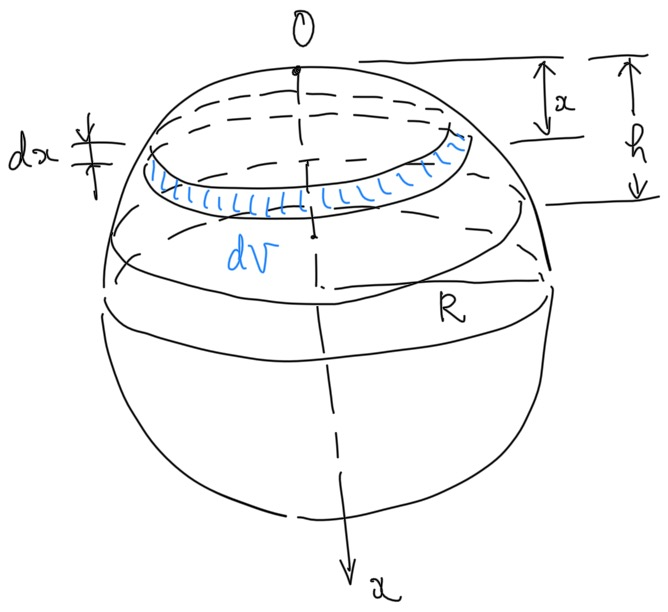
\includegraphics[width=.9\textwidth]{./images/ch6/topSp.jpg}
			\end{center}		
		\end{column}
		\begin{column}{.5\textwidth}
			\small 证:\it
			如图,体积微元
			$\d V=\pi[R^2-(R-x)^2]\d x=\pi(2Rx-x^2)\d x,$
			故球缺体积
			\begin{align*}
				V&=\dint_0^h\pi(2Rx-x^2)\d x\\
				&=\pi h^2\left(R-\df{h}3\right).
			\end{align*}
		\end{column}
	\end{columns}
\end{frame}

\begin{frame}
	\linespread{1.5}
	\ba{5.直线$y=x$将椭圆$x^2+3y^2=6y$分为两块,求两块的面积之比。
	}
	\pause
	
% 	\bigskip
	
	\begin{columns}
		\begin{column}{.45\textwidth}
			\begin{center}
				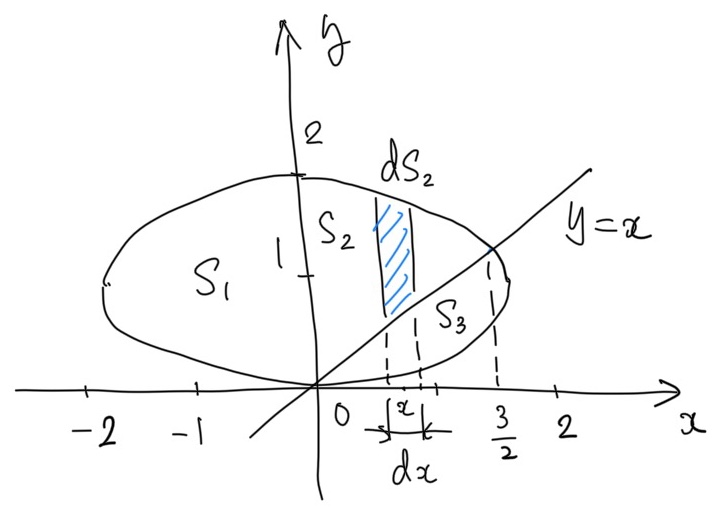
\includegraphics[width=.9\textwidth]{./images/ch6/ecXY.jpg}
			\end{center}		
		\end{column}
		\begin{column}{.55\textwidth}
			\small 要点:\it
			如图,
			\begin{align*}
				S_2&=\dint_0^{\frac32}\left(1+\sqrt{1-\df{x^2}3}-x\right)\d x\\
				&=\df34+\df{\sqrt3}6\pi.
			\end{align*}
			又$S_1=\sqrt3\pi$,故所求面积比为
			$$\df{S_1-S_2}{S_1+S_2}=\df{10\sqrt3\pi-9}
			{14\sqrt3\pi+9}$$
		\end{column}
	\end{columns}
\end{frame}

\begin{frame}
	\linespread{1.5}
	\ba{6.求曲线$y=\sqrt x$的一条切线,使之与该曲线及$x=0$、$x=2$
	共同所围面积最小。
	}
	\pause
	
% 	\bigskip
	
	\begin{columns}
		\begin{column}{.4\textwidth}
			\begin{center}
				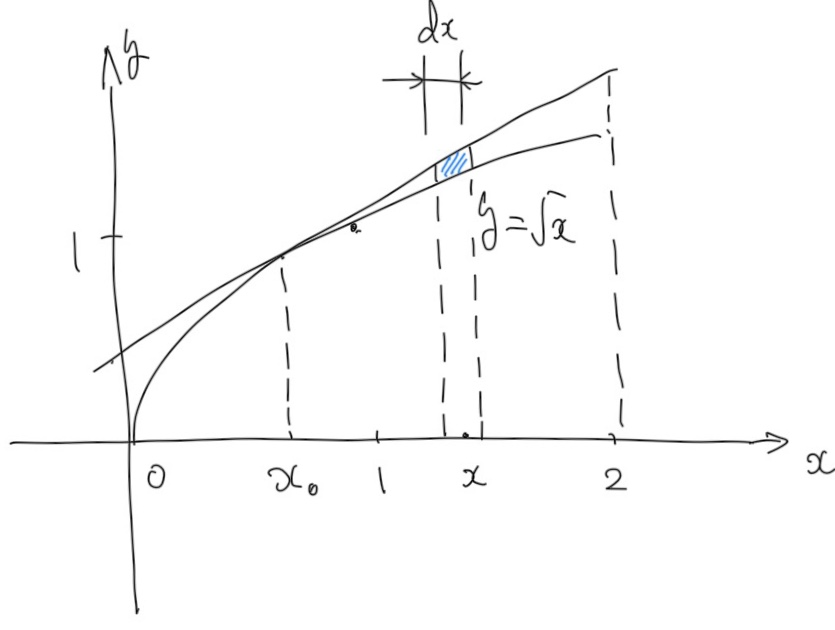
\includegraphics[width=\textwidth]{./images/ch6/ySqtXx.jpg}
			\end{center}		
		\end{column}
		\begin{column}{.6\textwidth}
			\small 解:\it
			如图,过曲线上一点$(x_0,\sqrt{x_0})$的切线为
			$y=\sqrt{x_0}+\df1{2\sqrt{x_0}}(x-x_0),$
			进而面积微元
			$\d S=\left[\df1{2\sqrt{x_0}}(x-x_0)+\sqrt{x_0}-\sqrt{x}\right]\d
			x$,$x\in[0,2]$。故所述面积
		\end{column}
	\end{columns}
	\small\it
	$$S=\dint_0^2\left[\df1{2\sqrt{x_0}}(x-x_0)+\sqrt{x_0}-\sqrt{x}\right]
	\d x=\df1{\sqrt{x_0}}+\sqrt{x_0}-\df{4\sqrt2}3.$$
	显然,当$x_0=1$时,该面积最小,此时对应切线为$y=\df12(x+1)$。
\end{frame}

\begin{frame}
	\linespread{1.5}
	\ba{8.求底面是半径为$R$的圆,而垂直于底面上一条固定直径的所有截面均为
	等边三角形的立体的体积。
	}
	\pause
	
	\bigskip
	
	\begin{columns}
		\begin{column}{.4\textwidth}
			\begin{center}
				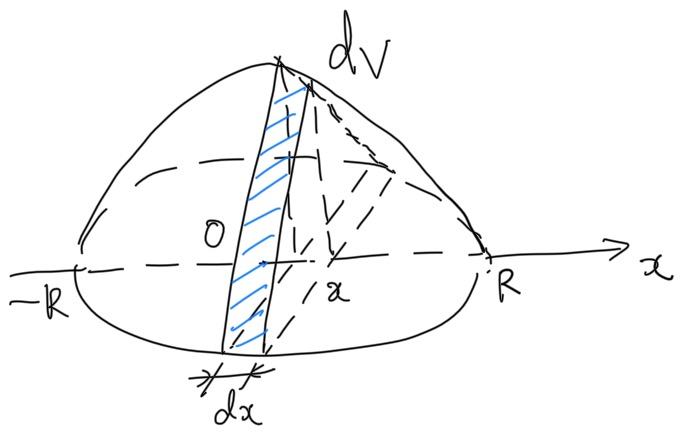
\includegraphics[width=\textwidth]{./images/ch6/rtSp.jpg}
			\end{center}		
		\end{column}
		\begin{column}{.6\textwidth}
			\small 解:\it
			如图,体积微元
			$$\d V=\sqrt3(R^2-x^2)\d x,\;x\in[-R,R],$$
			故所求体积
			$$V=\dint_{-R}^R\sqrt3(R^2-x^2)\d x=\df{4\sqrt3}3R^3.$$
		\end{column}
	\end{columns}
\end{frame}

\section{6.3 定积分的物理应用}

\begin{frame}
	\linespread{1.5}
	\ba{1.长度为$l$的细杆,均匀带电,总电量为$q\,(q<0)$,若在杆的延长线上,
	距离杆一端$x_0$处有一单位正电荷。现将单位正电荷从$x_0$处移动到无穷远,试求克服
	电场力所作的功。
	}
	\pause
	
	\begin{center}
		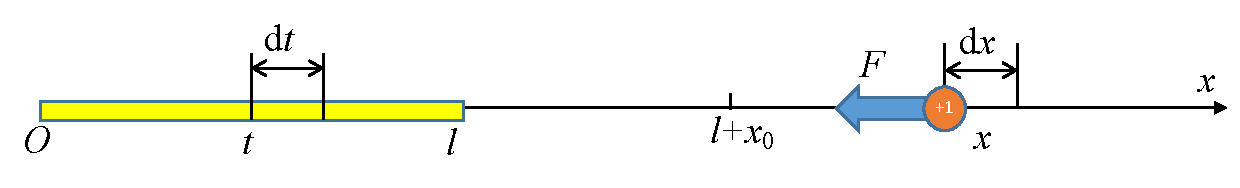
\includegraphics[width=.9\textwidth]{./images/ch6/eMove.pdf}
	\end{center}
	\small 解:\it
	如图,当单位正电荷位于$x(x>l)$处时,细杆上位置$t$处长度为$\d t$的一段对其产生的电场(吸引)力为
	$\d F=\df{kq\d t}{l(x-t)^2}$,$t\in[0,l]$
	故此时单位正电荷所受的总电场力为
	$$F=\dint_0^l\df{kq\d t}{l(x-t)^2}=\df{kq}l\left(\df1{x-l}-\df1x\right).$$
\end{frame}

\begin{frame}
	\linespread{1.5}
	\ba{1.长度为$l$的细杆,均匀带电,总电量为$q\,(q<0)$,若在杆的延长线上,
	距离杆一端$x_0$处有一单位正电荷。现将单位正电荷从$x_0$处移动到无穷远,试求克服
	电场力所作的功。
	}
	\pause
	
	\begin{center}
		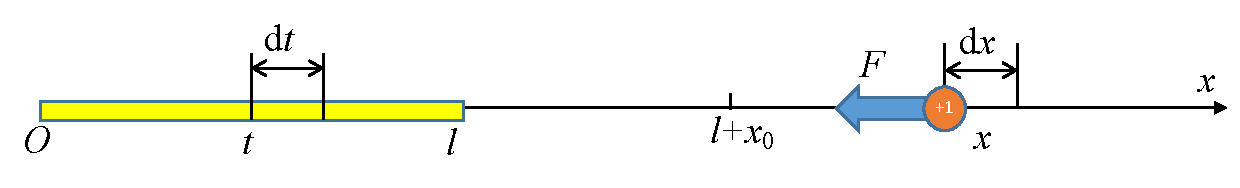
\includegraphics[width=.9\textwidth]{./images/ch6/eMove.pdf}
	\end{center}
	\small \it
	克服该力的作用,单位正电荷向远处移动$\d x$,需要做的功为
	$$\d W=F\d x=\df{kq}l\left(\df1{x-l}-\df1x\right)\d x,
	\quad x\in[l+x_0,+\infty)$$
	故所求克服电场力所需做的总功为
	$$W=\dint_{l+x_0}^{+\infty}\df{kq}l\left(\df1{x-l}-\df1x\right)\d x
	=\df{kq}l\ln\left(1+\df{l}{x_0}\right).$$
\end{frame}

\begin{frame}
	\linespread{2}
	\begin{columns}
		\begin{column}{.4\textwidth}
			\ba{2.星形线的参数方程为:$x=a\cos^3t,y=a\sin^3t$,设其上每一点处的密度
			等于其到原点距离的\underline{立方的}$k$倍,在原点处放置一单位质点,
			求星形线在第一象限的部分对该质点的引力。
			}	
		\end{column}
		\begin{column}{.6\textwidth}
			\begin{center}
				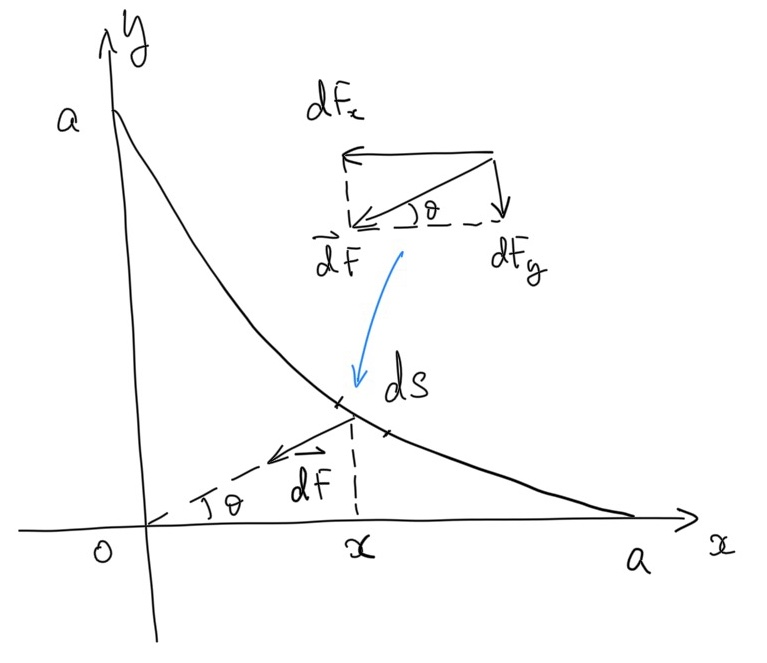
\includegraphics[width=.9\textwidth]{./images/ch6/starGr.jpg}
			\end{center}
		\end{column}
	\end{columns}
\end{frame}

\begin{frame}
	\linespread{1.5}
	\ba{3.边长为$a$和$b$的矩形薄板,与水面成角度$\theta$斜沉于水中,长边
	平行于水面,最低处深度为$h$,设$a<b$,水的密度$\rho=1$,求水对于薄板上侧
	的总压力。
	}
	\pause
	
	\bigskip
	
	\begin{columns}
		\begin{column}{.45\textwidth}
			\begin{center}
				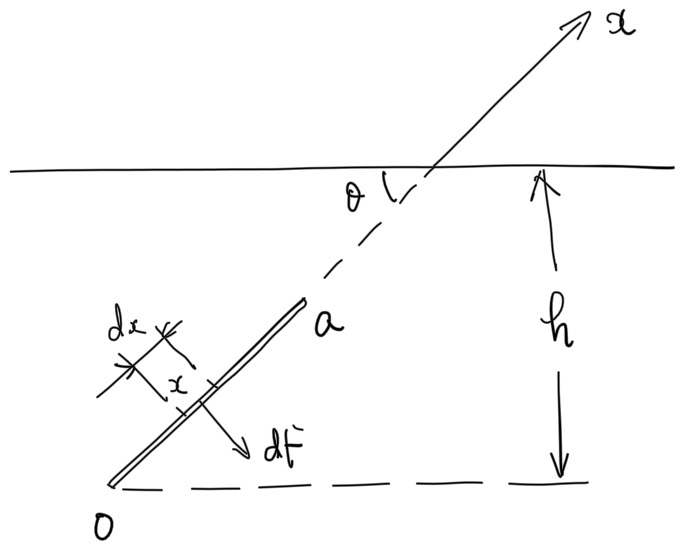
\includegraphics[width=\textwidth]{./images/ch6/waterPlane.jpg}
			\end{center}		
		\end{column}
		\begin{column}{.55\textwidth}
			\small 解:\it
			如图,压力微元
			$$\d F=g(h-x\sin\theta)b\d x,$$
			故所求压力
			\begin{align*}
				F&=\dint_0^ag(h-x\sin\theta)b\d x\\
				&=bg\left(ha-\df{a^2}2\sin\theta\right).
			\end{align*}
		\end{column}
	\end{columns}
\end{frame}

\begin{frame}
	\linespread{1.5}
	\ba{4.一个物体按照$x=t^3$作直线运动,已知其所受阻力等于其速度平方的$1.5$倍,
	求其从原点出发移动$1000$米时克服阻力所做的功。
	}
	\pause
	
	\begin{center}
		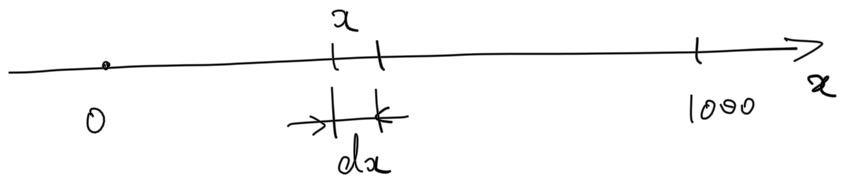
\includegraphics[width=.9\textwidth]{./images/ch6/moveSt.jpg}
	\end{center}
	\small 解:\it
	如图,功的微元$\d W=\df32(x'_t)^2\d x=\df{81}2t^6\d t$,故所求总功
	$$W=\dint_0^{10}\df{81}2t^6\d t=\df{81}{14}\times10^7.$$
\end{frame}

\begin{frame}
	\linespread{1.5}
	\ba{5.用铁锤将一铁钉击入木板,设木板对铁钉的阻力与铁钉已进入木板的深度成正比,
	已知第一次敲击后,铁钉进入木板$1$cm,假设每次敲击所做的功相同,问第二次敲击
	后,铁钉又将进入木板多少?
	}
	\pause
	
	\bigskip
	
	\begin{columns}
		\begin{column}{.35\textwidth}
			\begin{center}
				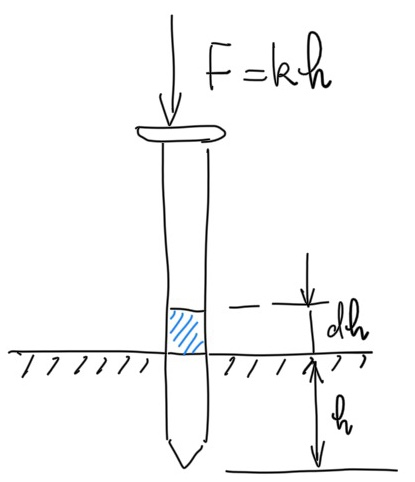
\includegraphics[width=\textwidth]{./images/ch6/nailSt.jpg}
			\end{center}		
		\end{column}
		\begin{column}{.65\textwidth}
			\small 解:\it
			如图,功的微元$\d W=kh\d h,$
			由已知第一次敲击时所做的功$W_1=\dint_0^1kh\d h=\df k2,$
			设第二次敲击后到达的深度为$h_2$,则与之相对应的功
			$$W_2=\dint_1^{h_2}kh\d h=\df k2(h^2_2-1)=W_1=\df k2,$$
			解得$h_2=\sqrt2$。故第二次敲击后,铁钉又将进入的深度为
			$\sqrt2-1$。
		\end{column}
	\end{columns}
\end{frame}

\begin{frame}
	\linespread{1.5}
	\ba{6.一个半径为$R$,圆心角为$\theta$的圆弧形细棒,其线密度为$\mu$,
	在圆心处放置一单位质点,问细棒对该质点的引力大小为多少?方向如何?
	}
	\pause
	
	\bigskip
	
	\begin{columns}
		\begin{column}{.4\textwidth}
			\begin{center}
				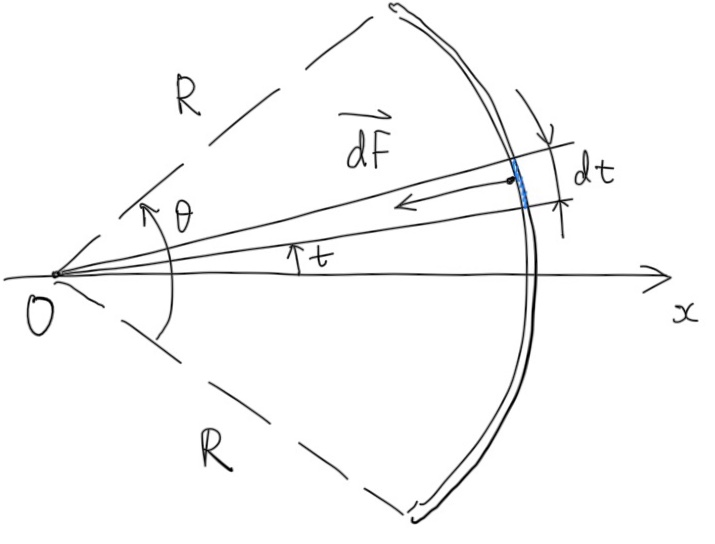
\includegraphics[width=\textwidth]{./images/ch6/theSphGr.jpg}
			\end{center}		
		\end{column}
		\begin{column}{.6\textwidth}
			\small 要点:\it
			引力微元
			$|\bm{\d F}|=\df{G\mu\d t}R,$,故
			\begin{align*}
				\d F_x&=|\bm{\d F}|\cos t=\df{G\mu\cos t\d t}R,\\
				\d F_y&=|\bm{\d F}|\sin t=\df{G\mu\sin t\d t}R,
			\end{align*}
			所求引力大小为$\df{2G\mu}{R}\sin\df{\theta}2$,沿$x$轴指向原点方向。
		\end{column}
	\end{columns}
\end{frame}

% % !Mode:: "TeX:UTF-8"

\titlepage

% \begin{frame}{说在前面}
% 	\linespread{1.5}
% 	  \begin{itemize}[<+-|alert@+>]
% 	    \item \ba{雷同!!!}
% 	    \item 本子太烂了就换本新的吧
% 	    \item 本子还不算特别烂的下学期请继续使用
% 	    \item 新本子:贴照片,写上姓名、专业、学号、籍贯
% 	  \end{itemize}
% \end{frame}

% \begin{frame}{需要注意的问题}
% 	\linespread{1.5}
% 	  \begin{itemize}%[<+-|alert@+>]
% 	    \item L'Hospital法则
% 	    \begin{itemize}
% 	      \item \it 只能应用于“$\df{\bm{0}}{\bm{0}}$”
% 	      和“$\df{\bm{\infty}}{\bm{\infty}}$”型
% 	      \item \it 及时使用无穷小代换进行简化
% 	      \item \it 不正规的符号:\b 
% 	      $\xlongequal{\footnotesize\mbox{“L”}}$、
% 	      $\xlongrightarrow{\footnotesize\mbox{“L'Hospital法则”}}$、
% 	      $\df{\bm{0}}{\bm{0}}$、$\df{\bm{\infty}}{\bm{\infty}}$
% 	    \end{itemize}
% 	    \item Taylor公式
% 	    \begin{itemize}
% 	      \item \it Taylor多项式不包含余项
% 	      \item \it 合并同次幂的系数
% 	      \item \it 尽量按照幂次由低到高排列,最后写余项
% 	    \end{itemize}
% 	  \end{itemize}
% \end{frame}

% \section{12.3 幂级数及其应用}

\begin{frame}
	\linespread{1.5}
	\ba{1.求下列函数项级数的收敛域:
	
	\bs
	
	(1)$\df x{1\cdot 3}+\df{x^2}{2\cdot3^2}++\df{x^3}{3\cdot3^3}
	+\ldots++\df{x^n}{n\cdot3^n}+\ldots$}
	
	\bigskip
	
	\small 解:\it
	因为
	$$\limn\sqrt[n]{\df1{n\cdot 3^n}}=\df13,$$
	故该级数的收敛区间为$(-3,3)$。
	
	又$x=3$时,级数为$\sumn\df1n$,发散;
	$x=-3$时,级数为$\sumn\df{(-1)^n}n$,收敛。
	故所求收敛域为$[-3,3)$。
\end{frame}

\begin{frame}
	\linespread{1.5}
	\ba{(2)$\sumn\df{(2x+1)^n}n$}
	
% 	\bigskip
	
	\small 解:\it
	令$y=2x+1$,考虑级数$\sumn\df{y^n}n$。因为$\limn\sqrt[n]{\df1n}=1$,
	故其收敛区间为$(-1,1)$。
	
	又$y=1$时,级数为$\sumn\df1n$,发散;
	$y=-1$时,级数为$\sumn\df{(-1)^n}n$,收敛。故级数$\sumn\df{y^n}n$
	的收敛域为$y\in[-1,1)$。相应地,原级数的收敛域为$x\in[-1,0)$。
\end{frame}

\begin{frame}
	\linespread{1.5}
	\ba{(3)$\sumn(-1)^n\df{x^{2n+1}}{2n}$}
	
% 	\bigskip
	
	\small 解:\it
	$\sumn(-1)^n\df{x^{2n+1}}{2n}=x\cdot\sumn(-1)^n\df{x^{2n}}{2n}$,
	由此可知原级数与级数$\sumn(-1)^n\df{x^{2n}}{2n}$同敛散。
	
	令$y=x^2$,考虑级数$\sumn(-1)^n\df{y^{n}}{2n}$。因为
	$\limn\sqrt[n]{\df1{2n}}=1$,故该级数的收敛区间为$(-1,1)$。
	相应地,级数$\sumn(-1)^n\df{x^{2n}}{2n}$与原级数的收敛区间均为$(-1,1)$。
	
	又$x=\pm1$时,原级数为$\sumn\df{(-1)^n}{2n}$,由Leibniz判别法,收敛。
	故原级数的收敛域为$[-1,1]$。
\end{frame}

\begin{frame}
	\linespread{1.5}
	\ba{(4)$\sumn\sin\df 1 {3n}\left(\df{3+x}{3-2x}\right)^n$}
	
% 	\bigskip
	
	\small 解:\it
	令$y=\df{3+x}{3-2x}$,考虑级数$\sumn y^n\sin\df1{3n}$。
	因为
	$$\limn\df{\sin\frac1{3n}}{\sin\frac1{3(n+1)}}=1,$$
	故该级数的收敛区间是$(-1,1)$。
	
	又$y=1$时,级数为$\sumn\sin\df1{3n}$,因为$\limn n\sin\df1{3n}=\df13$,
	故由比较判别法,级数发散;$y=-1$时,级数为$\sumn(-1)^n\sin\df1{3n}$,
	由Leibniz判别法,收敛。故级数$\sumn y^n\sin\df1{3n}$的收敛域为
	$[-1,1)$。求解不等式$-1\leq\df{3+x}{3-2x}<1$,
	可得$x\in(-\infty,0)\cup[6,+\infty)$,即为所求原级数的收敛域。\fin
\end{frame}

\begin{frame}
	\linespread{1.5}
	\ba{2.求下列级数的和函数:
	(1)$\sumn(-1)^{n-1}nx^{n-1}$}
	
% 	\bigskip
	
	\small 解:\it
	令$y=-x$,考虑级数$\sumn ny^{n-1}$,易得该级数的收敛域为$(-1,1)$。
	设其和函数为$S(y)$,于是当$y\in(-1,1)$时,
	$$\dint_0^yS(t)\d t=\dint_0^y\sumn nt^{n-1}\d t
	=\sumn \dint_0^ynt^{n-1}\d t=\sumn y^n=\df1{1-y}-1,$$
	进而可得
	$$S(y)=\df1{(1-y)^2}.$$
	综上,
	$$\sumn(-1)^{n-1}nx^{n-1}=\df1{(1+x)^2},\quad x\in(-1,1).$$
\end{frame}

\begin{frame}
	\linespread{1.5}
	\ba{(2)$\df1a+\df{2x}{a^2}+\ldots+\df{nx^{n-1}}{a^n}+\ldots$,其中$a>0$.}
	
	\bigskip
	
	\small 解:\it
	该级数即为$\df1a\sumn n\left(\df xa\right)^{n-1}$,易得其收敛域为$(-a,a)$。
	记$y=\df xa$,由$(1)$的结果可得
	\begin{align*}
		\df1a\sumn n\left(\df xa\right)^{n-1}
		&=\df1a\sumn ny^{n-1}=\df1a\df1{(1-y)^2}\\
		&=\df1a\df1{\left(1-\frac
		xa\right)^2} =\df{a}{(a-x)^2}.
	\end{align*}
	即为所求。
\end{frame}

\begin{frame}
	\linespread{1.5}
	\ba{(3)$\sumn[0]\df{x^{2n+1}}{n!}$}
	
	\bigskip
	
	\small 解:\it
	该级数的收敛域为$(-\infty,+\infty)$。令$y=x^2$
	$$\sumn[0]\df{x^{2n+1}}{n!}=x\sumn[0]\df{x^{2n}}{n!}
	=x\sumn[0]\df{y^n}{n!}.$$
	级数$\sumn[0]\df{y^n}{n!}$当$y\in(-\infty,+\infty)$时收敛于$e^y$。
	由此即知
	$$\sumn[0]\df{x^{2n+1}}{n!}=xe^{x^2},\quad x\in(-\infty,+\infty).$$
	\fin
\end{frame}

\begin{frame}
	\linespread{1.5}
	\ba{3.将下列函数展开成Maclaurin级数,并求其收敛域:
	
	(1)$f(x)=\df1{x^2-4x+3}$}
	
	\bigskip
	
	\small 解:\it
	\begin{align*}
		\df1{x^2-4x+3}&=\df12\left(\df1{1-x}-\df13\df1{1-\frac x3}\right)\\
		&=\df12\left(\sumn[0]x^n-\df13\sumn[0]\df{x^n}{3^n}\right)\\
		&=\df12\sumn[0]\left(1-\df1{3^{n+1}}\right)x^n.
	\end{align*}
	该级数的收敛域为$[-1,1)$。
\end{frame}

\begin{frame}
	\linespread{1.5}
	\ba{(2)$f(x)=\df 1{1+x+x^2}$}
	
	\bigskip
	
	\small 解:\it
	\begin{align*}
		\df 1{1+x+x^2}
		&=\df{1-x}{1-x^3}=(1-x)\sumn[0]x^{3n}\\
		&=1-x+x^3-x^4+x^6-x^7+\ldots+x^{3n}-x^{3n+1}+\ldots.
	\end{align*}
	注意到级数$\sumn[0]x^{3n}$的收敛域为$(-1,1)$,故以上级数的收敛域为$(-1,1)$。\fin
\end{frame}

\begin{frame}
	\linespread{1.5}
	\ba{4.将函数$f(x)=\df1{\sqrt{3+2x-x^2}}$展开成$x=1$处的幂级数,并求其收敛区间。}
	
	\bigskip
	
	\small 解:\it
	\begin{align*}
		f(x)
		&=\df12\left[1-\left(\df{x-1}2\right)^2\right]^{-\frac12}
		=\df12\sumn[0]{\left(\begin{array}{c}
			-\frac12 \\ n
		\end{array}\right)}\left[-\left(\df{x-1}2\right)^2\right]^n\\
		&=\sumn[0]\df{(2n-1)!!}{2^{2n+1}(2n)!!}(x-1)^{2n}
	\end{align*}
	注意到
	$$\limn\df{\frac{(2n+1)!!}{2^{2n+3}(2n+2)!!}}{\frac{(2n-1)!!}{2^{2n+1}(2n)!!}}=\df12,$$
	故所得级数的收敛半径为$2$,相应地收敛区间为$(-1,3)$。
	\fin
\end{frame}

\begin{frame}
	\linespread{1.5}
	\ba{5.已知$f_n(x)\;(n\in\mathbb{Z}^+)$满足
	$$f'_n(x)=f_n(x)+x^{n-1}e^x,$$
	且$f_n(1)=\df en$,求级数$\sumn f_n(x)$的和。}
	
	\bigskip
	
	\small 解:\it
	由已知等式,可得
	$$\left[f_n(x)e^{-x}\right]'=x^{n-1},$$
	进而可知
	$$f_n(x)=\left(\df{x^n}n+C\right)e^x.$$
	注意到$f_n(1)=\df en$,可得$C=0$,故$f_n(x)=\df{x^n}ne^x$。
\end{frame}

\begin{frame}
	\linespread{1.5}
	\small\it
	
	$$\sumn f_n(x)=\sumn\df{x^n}ne^x=e^x\sumn\df{x^n}n.$$
	
	考虑级数$\sumn\df{x^n}n$,易得其收敛域为$[-1,1)$。设其和函数为$S(x)$,则
	$$S'(x)=\left[\sumn\df{x^n}n\right]'
	=\sumn\left[\df{x^n}n\right]'=\sumn x^{n-1}=\df1{1-x}.$$
	从而
	$$S(x)=\dint_0^x\df1{1-t}\d t=-\ln|1-x|,\quad x\in[-1,1),$$
	进而
	$$\sumn f_n(x)=-\df{e^x}\ln|1-x|,\quad x\in[-1,1).$$
	\fin
\end{frame}

\begin{frame}{出现的问题}
	\linespread{1.5}
	  \begin{itemize}%[<+-|alert@+>]
	    \item 作业进度慢!
	    \item 概念问题
	    \begin{itemize}
	      \item \b\it 幂级数展开不熟练
	      \item \b\it Maclaurin级数和关于$(x-x_0)$的幂级数分不清
	    \end{itemize}
	    \item 过程不规范或不完整
	    \begin{itemize}
	      \item \b\it 求收敛域要单独讨论端点的敛散性
	      \item \b\it 相同幂次的项要合并,并按幂次从小到大排列
	      \item \b\it 书写潦草随意\pause
	    \end{itemize}
	    \item \ba{雷同!!!}
	  \end{itemize}
\end{frame}

% \begin{frame}
% 	\linespread{1.5}
% 	\ba{3.设$D$是由曲线$y=\sin x+1$与三条直线$x=0,x=\pi,y=0$
% 	所围成的曲边梯形,求$D$绕$x$轴旋转一周所围成的旋转体的体积。
% 	}
% 	\pause
% 	
% % 	\bigskip
% 	
% 	\begin{columns}
% 		\begin{column}{.5\textwidth}
% 			\begin{center}
% 				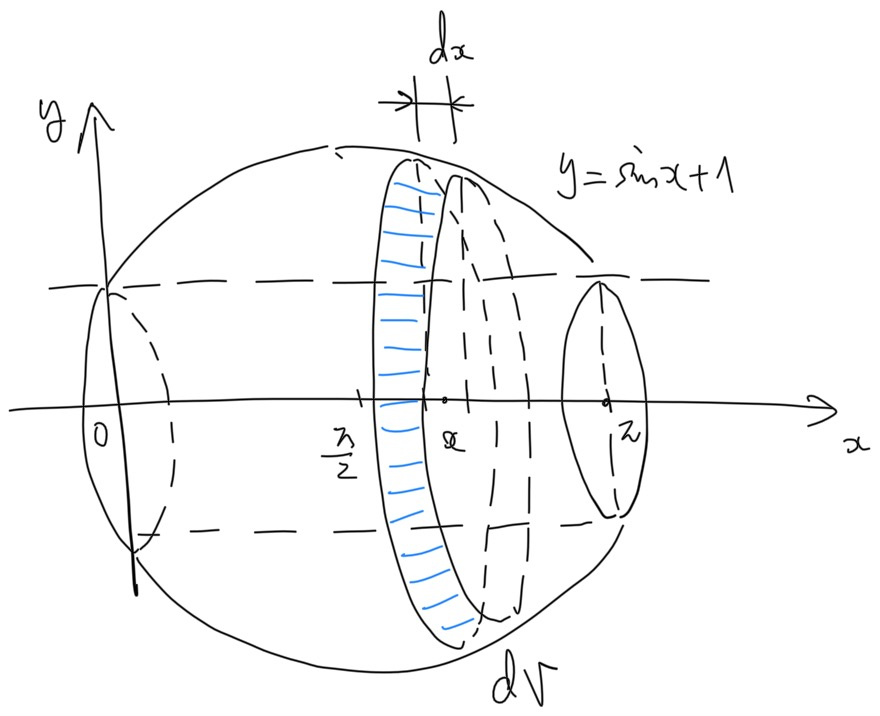
\includegraphics[width=.9\textwidth]{./images/ch6/sinx1cs.jpg}
% 		% 		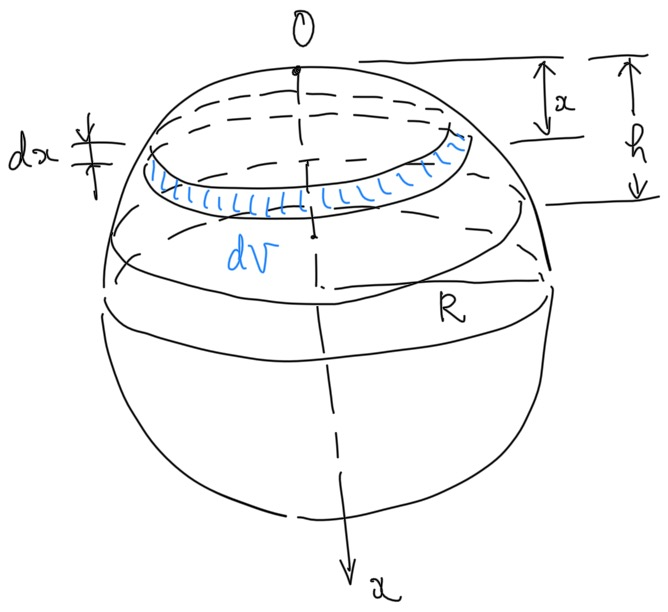
\includegraphics[width=6cm]{./images/ch6/topSp.jpg}
% 			\end{center}		
% 		\end{column}
% 		\begin{column}{.5\textwidth}
% 			\small 解:\it
% 			如图,体积微元$\d V=\pi y^2\d x$,	故所求体积
% 			$$
% 				V=\dint_0^{\pi}\pi(\sin x+1)^2\d x=\df32\pi^2.
% 			$$
% 		\end{column}
% 	\end{columns}
% \end{frame}

% % !Mode:: "TeX:UTF-8"

\titlepage

\begin{frame}{说在前面}
	\linespread{1.5}
	  \begin{itemize}[<+-|alert@+>]
	    \item \ba{雷同!!!}
	    \item \ba{雷同!!!}
	    \item \ba{雷同!!!}
	  \end{itemize}
\end{frame}

% \begin{frame}{需要注意的问题}
% 	\linespread{1.5}
% 	  \begin{itemize}%[<+-|alert@+>]
% 	    \item L'Hospital法则
% 	    \begin{itemize}
% 	      \item \it 只能应用于“$\df{\bm{0}}{\bm{0}}$”
% 	      和“$\df{\bm{\infty}}{\bm{\infty}}$”型
% 	      \item \it 及时使用无穷小代换进行简化
% 	      \item \it 不正规的符号:\b 
% 	      $\xlongequal{\footnotesize\mbox{“L”}}$、
% 	      $\xlongrightarrow{\footnotesize\mbox{“L'Hospital法则”}}$、
% 	      $\df{\bm{0}}{\bm{0}}$、$\df{\bm{\infty}}{\bm{\infty}}$
% 	    \end{itemize}
% 	    \item Taylor公式
% 	    \begin{itemize}
% 	      \item \it Taylor多项式不包含余项
% 	      \item \it 合并同次幂的系数
% 	      \item \it 尽量按照幂次由低到高排列,最后写余项
% 	    \end{itemize}
% 	  \end{itemize}
% \end{frame}

\section{7.1 概念与应用}

\begin{frame}
	\linespread{1.5}
	\ba{1.请给出如下通解对应的微分方程,并给出其满足给定初值条件的特解:
	
	(1)$y=x^2+C_1x+C_2$,其中$C_1,C_2$为任意常数,$y(0)=y'(0)=1$;}
	
	\bigskip
	
	\small 解:\it
	原方程两边对$x$连续两次求导,可得
	$$y'=2x+C_1,\quad y''=2,$$
	即为所求方程。
	
	将$y(0)=y'(0)=1$分别带入通解和上述第一个方程可得$C_1=C_2=1$,故
	所求特解为$y=x^2+x+1$。
\end{frame}

\begin{frame}
	\linespread{1.5}
	\ba{$y=\df{1+Ce^t}{1-Ce^t}$,其中$C$为任意常数,$y(0)=2$;}
	
% 	\bigskip
	
	\small 解:\it
	原方程可化为
	$$C=\df{y-1}{y+1}e^{-t},$$
	两边对$t$求导,可得
	$$0=\df{2y'-y^2+1}{(y+1)^2}e^{-t},$$
	从而可得
	$$2y'-y^2+1=0,\quad(y\ne-1),$$
	即为所求方程。
	
	将$y(0)=2$带入通解可得$C=\frac13$,从而所求特解为
	$y=\df{3+e^t}{3-e^t}$。
\end{frame}

\begin{frame}
	\linespread{1.5}
	\ba{$y=(C_1+C_2x)e^x$,其中$C_1,C_2$为任意常数,$y(0)=0,y'(1)=1$.}
	
% 	\bigskip
	
	\small 解:\it
	原方程可化为
	$$ye^{-x}=C_1+C_2x,$$
	两边对$x$连续两次求导,可得
	$$(y'-y)e^{-x}=C_2,\quad
	(y''-2y'+y)e^{-x}=0.$$
	因为$e^{-x}\ne0$,故所求方程即为
	$$y''-2y'+y=0.$$
	
	又将$y(0)=0,y'(1)=1$带入通解和前述第一个方程中,可得
	$C_1=0,C_2=\frac1{2e}$,从而所求特解为$y=\frac12xe^{x-1}$。
	\fin
\end{frame}

\begin{frame}
	\linespread{1.5}
	\ba{2.设河边点$O$的正对岸为点$A$,河宽$h$,两岸平行,水流速度恒定为$a$。
	一只鸭子从点$A$游向点$O$,游动过程中其始终朝向$O$点。已知鸭子在
	静水中的游速为$b(b>a)$,以$O$为原点,水流方向为$x$轴,垂直于水流
	过河的方向为$y$轴,试给出鸭子的运动轨迹所满足的微分方程初值问题。}
	
% 	\bigskip

	\begin{center}
		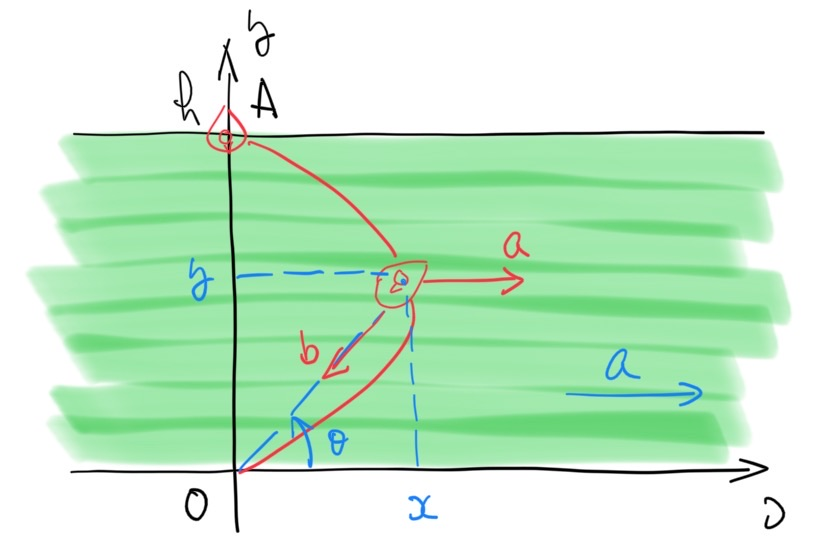
\includegraphics[width=0.6\textwidth]{./images/ch7/duck.jpg}
	\end{center}
\end{frame}

\begin{frame}
	\linespread{1.5}	
	\small 解:\it
	在鸭子运动轨迹上任一点$(x,y)$处,其运动满足
	$$x'_t=a-b\cos\theta,\quad y'_t=-b\sin\theta,$$
	其中
	$$\sin\theta=\df{y}{\sqrt{x^2+y^2}},\quad
	\cos\theta=\df{x}{\sqrt{x^2+y^2}},$$
	故
	$$y'_x=\df{y'_t}{x'_t}=\df{-by}{a\sqrt{x^2+y^2}-bx},$$
	显然$y(0)=h$,故所求初值问题为
	$$
		\left\{\begin{array}{l}
			y'=\df{-by}{a\sqrt{x^2+y^2}-bx},\\
			y(0)=h.
		\end{array}\right.
	$$
	\fin
\end{frame}

\section{7.2 一阶微分方程的解法}

\begin{frame}
	\linespread{1.5}
	\ba{1.求解下列微分方程:
	
	(1)$xy'-y+\sqrt{x^2-y^2}=0,(x>0)$}
	
	\bigskip
	
	\small 解:\it
	令$z=\frac yx$,则原方程可化为
	$$xz'+\sqrt{1-z^2}=0.$$
	当$\sqrt{1-z^2}\ne 0$时,该方程分离变量,解得$z=\sin(-\ln x+C)$。
	当$\sqrt{1-z^2}=0$时,方程有解$y=\pm x$。
	
	综上,原方程的解为
	$$y=x\sin(\ln x+C),\;(x\in\mbb{R})
	\quad\mbox{或}\quad y=\pm x.$$
\end{frame}

\begin{frame}
	\linespread{1.5}
	\ba{(2)$y'=(x+y)^2$}
	
	\bigskip
	
	\small 解:\it
	令$z=x+y$,则原方程可化为
	$$z'-1=z^2,$$
	该方程分离变量,解得$z=\tan(x+C)$,进而原方程的解为
	$$x+y=\tan(x+C),\;(C\in\mbb{R}).$$
\end{frame}

\begin{frame}
	\linespread{1.5}
	\ba{(3)$x\ln x\d y+(y-\ln x)\d x=0$ }
	
	\bigskip
	
	\small 解:\it
	令$u=\ln x$,则原方程可化为
	$$u\d y+(y-u)\d u=0,$$
	该方程是一个齐次方程(也是一个全微分方程),可解得
	$2yu-u^2=C$,故原方程的解为
	$$(2y-\ln x)\ln x=C,\;(C\in\mbb{R}).$$
\end{frame}

\begin{frame}
	\linespread{1.5}
	\ba{(4)$3y'+y=(1-x)y^4$}
	
	\bigskip
	
	\small 解:\it
	该方程为Bernoulli方程。当$y\ne0$时,令
	$z=y^{-3}$,则原方程可化为
	$$-z'+z=1-x,$$
	该方程为一阶非齐次线性微分方程,可解得
	$z=-x+Ce^x$。显然$y=0$是方程的特解。综上原方程的解为
	$$y^3(-x+Ce^x)=1,\;(C\in\mbb{R}),\;\mbox{或}\;y=0.$$
	\fin
\end{frame}

\begin{frame}
	\linespread{1.5}
	\ba{2.某湖泊的水量为$V$,每年排入湖内的污水和净水量均为$V/6$,且湖内的总水量不变。
	已知1999年底湖内的污染物含量为$5m_0$。为了治理污染,从2000初开始,限定排入
	湖中的污水中污染物浓度不得超过$m_0/V$。问至少需要经过多少年,
	湖内的污染物含量能够降至$m_0$以下?(注:假设湖水中的污染物浓度是均匀分布的。)}
	
	\bigskip
	
	\small 解:\it
	设$m(t)$为自2000年起第$t$年时湖内的污染物总量,则
	$$m'=\df{m_0}6-\df{m}3,$$
	且$m(0)=5m_0$。
\end{frame}

\begin{frame}
	\linespread{1.5}
	\small\it
	
	设$m(t)$为自2000年起第$t$年时湖内的污染物总量,则
	$$m'=\df{m_0}6-\df{m}3,$$
	且$m(0)=5m_0$。解之可得
	$$m=\df{m_0}2\left(1+9e^{-\frac13t}\right).$$
	令$m<m_0$,可得$t>3\ln9\approx6.59$,故大约7年后,湖水中的污染物含量可以
	降至$m_0$以下。\fin
\end{frame}

\begin{frame}
	\linespread{1.5}
	\ba{3.已知$f(0)=0,f(1)=1$,且当$x\in(0,1)$时,$f''(x)<0$。任取曲线
	$y=f(x)$上一点$(x,f(x)),\;(x\in(0,1))$,该点与原点的连线与曲线所围图形
	面积为$x^2$,求$f(x)$。}
	
	\begin{center}
		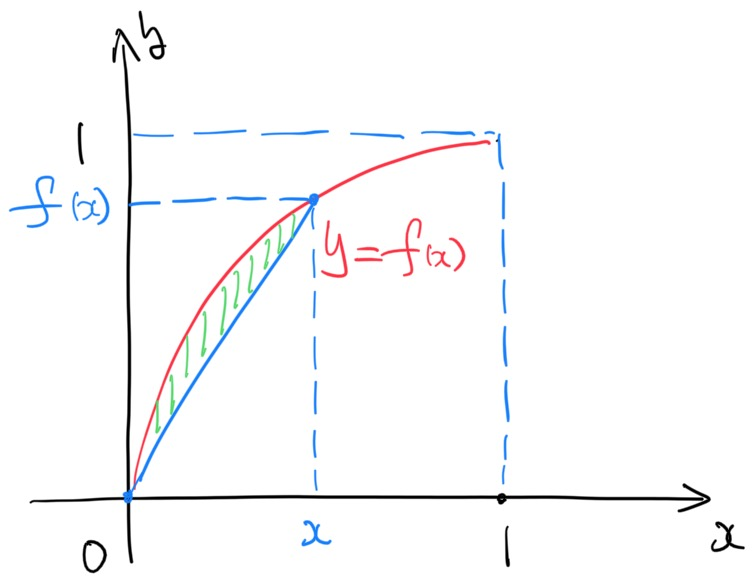
\includegraphics[width=0.6\textwidth]{./images/ch7/fxx2.jpg}
	\end{center}
\end{frame}

\begin{frame}
	\linespread{1.5}	
	\small 解:\it
	由已知
	$$\dint_0^xf(t)\d t-\df12xf(x)=x^2,\quad x\in[0,1],$$
	两边求导,整理得
	$$f(x)-xf'(x)=4x.$$
	该方程为一阶非齐次线性微分方程,解之得
	$$f(x)=(-4\ln x+C)x,\;(C\in\mbb{R},x\in(0,1)),$$
	带入$f(1)=1$,可解得$C=1$,从而所求曲线的方程为
	$$f(x)=\left\{\begin{array}{ll}
		0,& x=0,\\
		(-4\ln x+1)x,& x\in(0,1].
	\end{array}\right.$$
	\fin
\end{frame}

\begin{frame}
	\linespread{1.5}
	\ba{4.某学生将乘积的导数公式错误地记作$(fg)'=f'g'$,然而在一次求导时居然
	得到了正确的结果。目前知道他使用的$f(x)=e^{x^2}\,(x>1/2)$,
	问他用到的$g(x)$可能是什么?}
	
	\bigskip
	
	\small 解:\it
	由已知
	$$(e^{x^2}g(x))'=(e^{x^2})'g'(x),$$
	展开化简可得
	$$2xg=(2x-1)g',$$
	该方程分离变量,求解可得
	$$g(x)=Ce^x\sqrt{2x-1},\;(x>\frac12).$$
	\fin
\end{frame}

% \begin{frame}{出现的问题}
% 	\linespread{1.5}
% 	  \begin{itemize}%[<+-|alert@+>]
% 	    \item 作业进度慢!
% 	    \item 概念问题
% 	    \begin{itemize}
% 	      \item \b\it 幂级数展开不熟练
% 	      \item \b\it Maclaurin级数和关于$(x-x_0)$的幂级数分不清
% 	    \end{itemize}
% 	    \item 过程不规范或不完整
% 	    \begin{itemize}
% 	      \item \b\it 求收敛域要单独讨论端点的敛散性
% 	      \item \b\it 相同幂次的项要合并,并按幂次从小到大排列
% 	      \item \b\it 书写潦草随意\pause
% 	    \end{itemize}
% 	    \item \ba{雷同!!!}
% 	  \end{itemize}
% \end{frame}

% \begin{frame}
% 	\linespread{1.5}
% 	\ba{3.设$D$是由曲线$y=\sin x+1$与三条直线$x=0,x=\pi,y=0$
% 	所围成的曲边梯形,求$D$绕$x$轴旋转一周所围成的旋转体的体积。
% 	}
% 	\pause
% 	
% % 	\bigskip
% 	
% 	\begin{columns}
% 		\begin{column}{.5\textwidth}
% 			\begin{center}
% 				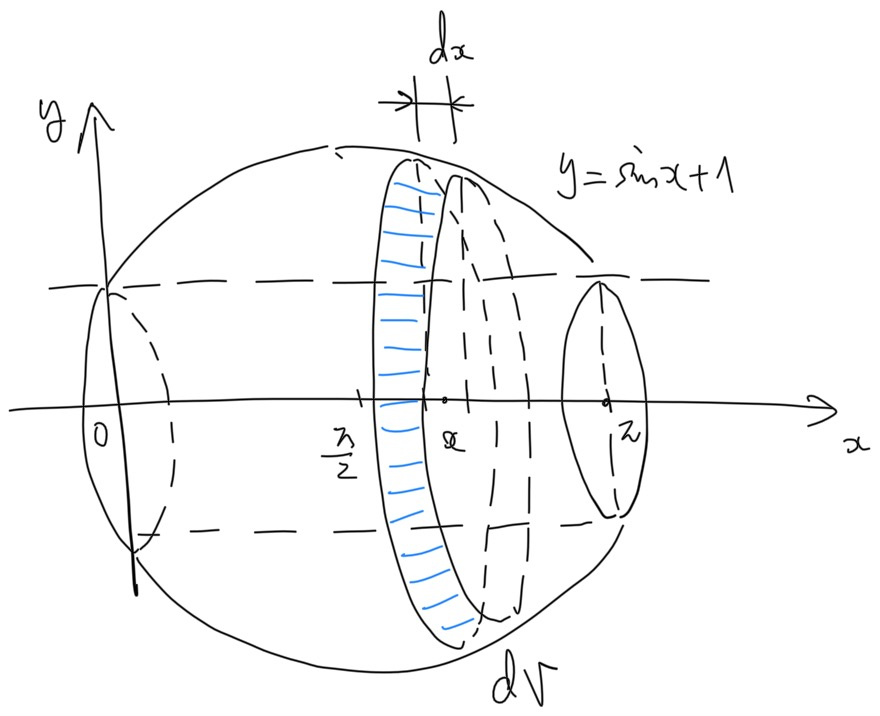
\includegraphics[width=.9\textwidth]{./images/ch6/sinx1cs.jpg}
% 		% 		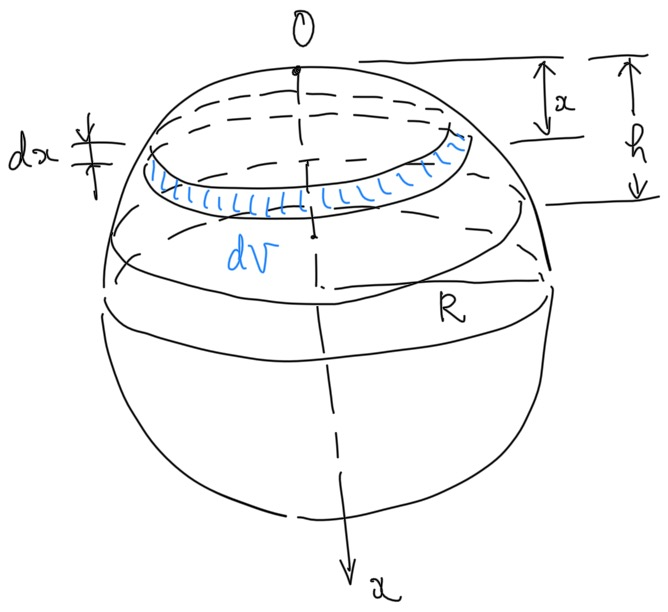
\includegraphics[width=6cm]{./images/ch6/topSp.jpg}
% 			\end{center}		
% 		\end{column}
% 		\begin{column}{.5\textwidth}
% 			\small 解:\it
% 			如图,体积微元$\d V=\pi y^2\d x$,	故所求体积
% 			$$
% 				V=\dint_0^{\pi}\pi(\sin x+1)^2\d x=\df32\pi^2.
% 			$$
% 		\end{column}
% 	\end{columns}
% \end{frame}

% % !Mode:: "TeX:UTF-8"

\titlepage

\begin{frame}
	\frametitle{知识点回顾}
	\linespread{1.5}
	\it
	  \begin{itemize}
 	    \item 微分方程及其解(通解、特解)的概念
	    \item 一阶微分方程的解法与常用技巧
	    \item 可降阶的二(高)阶微分方程
	    \item 二阶线性微分方程解的结构
	    \item 求解二阶常系数齐次线性微分方程的特征方程法
	    \item 求解特定二阶常系数非齐次线性微分方程的待定系数法
	  \end{itemize}
\end{frame}

\section{补充例题}

\subsection{二阶线性微分方程}

% \section{问题讨论}

% \begin{frame}{问题讨论}
% 	\linespread{1.5}
% 	\alert{问:}已知$n$阶线性微分方程的$n$个解,
% 	能否写出这个微分方程及其通解?\pause\\[1ex]
% 	
% 	\alert{答:}{\it 不一定。}\pause 除非{\it\b 
% 	这$n$个解恰为$n$阶齐次线性微分方程的线性无关的特解。} \pause 
% 	
% 	\bigskip
% 	\alert{问:}适当确定微分方程通解中的参数值,可以得到其任意的特解?\pause \\[1ex]
% 	
% 	\alert{答:}{\it 错!有些特解无法用统一的通解形式来表达。}\pause {\it 例如:}{\b $y'=\sin x\cos^2y$}.
% \end{frame}

\begin{frame}{问答题}
	\linespread{1.2}
	\alert{问:}$y_1=(x-1)^2$和$y_2=(x+1)^2$都是方程
	$$(x-1)^2y''-2xy'+2y=0,$$
	和
	$$2yy''-(y')^2=0$$
	的解。但二者的线性组合
	$$y=C_1(x-1)^2+C_2(x+1)^2,\;(C_1,C_2\in\mathbb{R})$$
	却仅能满足前一个方程,为什么?\pause 
	
	\alert{答:}{\it\b 第二个方程不是线性方程!}
\end{frame}

\begin{frame}{填空}
	\linespread{1.5}
	\alert{例:}$y''+4y'+4y=1$的通解为
	\underline{\uncover<2->{\;\b{$(C_1+C_2x)e^{-2x}+1/4$}}\;}.\\[1em]
	
	\alert{例:}设$e^x(C_1\cos x+C_2\sin x)$为首项系数为$1$的某二阶常系数
	齐次线性微分方程的通解,则该微分方程为
	\underline{\uncover<3->{\;\b{$y''-2y'+2y=0$}}\;}.\\[1em]
	
	\alert{例:}设$\cos x$与$xe^x$分别为某$n$阶常系数齐次线性微分方程的两个解,
	则最小的$n=$\underline{\uncover<4->{\;\b{$4$}}\;},相应的首项
	系数为$1$的方程为\underline{\uncover<5->{\;\b{$
	y^{(4)}-2y^{(3)}+2y''-2y'+y=0$}\;}}
	
% 	方程$xy''-2xy'+2y=x\ln x$的通解为
% 	为\underline{\uncover<6->{\;\b{$
% 	C_1x+C_2x^2-\left(\df12\ln^2x+\ln x\right)x$}\;}}
\end{frame}

\begin{frame}
	\linespread{1.2}
	\pause\alert{提示:}\it\b 
	特征方程的复根总是成对出现,故$\cos x$若为方程的解,$\sin x$也必为其解,
	对应的特征根为$r=\pm i$。
	
	又若$xe^x$为齐次线性微分方程的特解,则$r=1$必为对应特征方程的一个重根,
	进而可知$e^x$也是方程的解。
	
	综上,方程的特征根为$r=\pm i$和$r=1$(二重),于是特征方程为
	$$(r+i)(r-i)(r-1)^2=r^4-2r^3+2r^2-2r+1=0,$$
	由此易得原方程。
\end{frame}

\begin{frame}{选择}
	\linespread{1.3}
	\alert{例:}设$y_1(x),y_2(x),y_3(x)$为方程
	$$y''+p(x)y'+q(x)y=f(x)$$
	的三个线性无关的解,$C_1,C_2$为任意常数,则该非齐次线性微分方程的通解为
	(\underline{\uncover<2->{\;\b{C}}\;})
	\begin{enumerate}[(A)]
	  \item $(C_1+C_2)y_1+(C_2-C_1)y_2+(1-C_2)y_3$
	  \item $(C_1+C_2)y_1+(C_2-C_1)y_2+(C_1-C_2)y_3$
	  \item $C_1y_1+(C_2-C_1)y_2+(1-C_2)y_3$
	  \item $C_1y_1+(C_2-C_1)y_2+(C_1-C_2)y_3$
	\end{enumerate}
\end{frame}

\begin{frame}{选择}
	\linespread{1.5}
	\alert{例:}下列可能为方程$y''+4y=e^{3x}+x\sin 2x$的特解的是
	(\underline{\uncover<2->{\;\b{A}}\;})
	\begin{enumerate}[(A)]
	  \item $Ae^{3x}+x[(Bx+C)\cos2x+(Dx+E)\sin2x]$
	  \item $Ae^{3x}+(Bx+C)\cos2x+(Dx+E)\sin2x$
	  \item $Axe^{3x}+x[(Bx+C)\cos2x+(Dx+E)\sin2x]$
	  \item $Axe^{3x}+(Bx+C)\cos2x+(Dx+E)\sin2x$
	\end{enumerate}
	\pause\alert{提示:}\it\b 利用叠加原理,分别构造$e^3x$和$x\sin2x$
	对应的特解,再相加。
\end{frame}

\begin{frame}{选择}
	\linespread{1.3}
	\alert{例:}已知$xe^x+e^{2x}$和$xe^x+e^{-x}$是二阶常系数非齐次线性微分方程的两个解,
	则此方程为
	(\underline{\uncover<2->{\;\b{}}\;})
	\begin{enumerate}[(A)]
	  \item $y''-2y'+y=e^{2x}$
	  \item $y''-y'-2y=xe^{x}$
	  \item $y''-y'-2y=e^x-2xe^{x}$
	  \item $y''-y=e^{2x}$
	\end{enumerate}
	\pause\alert{提示:}\it\b 显然$e^{2x}-e^{-x}$为对应齐次方程的解,其中
	的两个函数线性无关,故分别为齐次方程的特解,进而特征根$r_1=2,r_2=-1$。
\end{frame}

\begin{frame}{选择}
	\linespread{1.3}
	\alert{例:}方程$y''+by'+y=0$的每个解都在$x>0$上有界,则实数$b$的取值范围是
	(\underline{\uncover<2->{\;\b{A}}\;})
	\begin{enumerate}[(A)]
	  \item $[0,+\infty)$
	  \item $(-\infty,0]$
	  \item $(-\infty,2)$
	  \item $(2,+\infty)$
	\end{enumerate}
	\pause\alert{提示:}\it\b 对照二阶常系数齐次线性方程的各种解的形式,可得
	当通解中的指数函数$e^{\lambda x}$满足$\lambda<0$时,即有所有的解有界。
	利用韦达定理可推出$b<0$。又$b=0$时,解方程可知也满足要求。
\end{frame}

\begin{frame}{解答题}
	\linespread{1.2}
	\alert{例:}求方程$y''+2y'+2y=2e^{-x}\cos^2\df x2$的通解.
	
	\pause\alert{提示:}\it\b 
	$$2e^{-x}\cos^2\df x2=e^{-x}+e^{-x}\cos x,$$
	利用叠加原理分别求解两个常系数非齐次线性微分方程。
\end{frame}

\begin{frame}{解答题}
	\linespread{1.5}
	\alert{例:}设二阶常系数线性微分方程
	$y''+\alpha y'+\beta y=\gamma e^x$
	的一个解为$y=e^{2x}+(1+x)e^x$,试确定其中的常数$\alpha,\beta,\gamma$.
	
	\pause\alert{提示:}\it\b 由解的结构,$e^{2x},e^x,xe^x$中有两个为齐次方程
	的特解,另一个为非齐次方程的特解。若$xe^x$为齐次方程的解,则$e^x$也是,此时非齐次
	方程的特解形如$Ax^2e^x$,显然$e^{2x}$不具有这种形式。故$xe^x$必为非齐次方程的特解,
	从而$e^{2x},e^x$为齐次方程的解。由此可得到对应的特征方程,进而
	进一步可解出$\alpha=-3,\beta=2,\gamma=-1$。
\end{frame}

\begin{frame}{解答题}
	\linespread{1.2}
	\alert{例:}利用变换$x=e^t$求解如下方程
	$$x^2\df{\d^2y}{\d x^2}+3x\df{\d y}{\d x}+5y=16x\ln x.$$
	
	\pause\alert{提示:}\it\b 
	$$y''_{tt}+2y'_t+5y=16te^{t}$$
	\pause \ba{请自行阅读教材第七章第九节“Euler方程”}
\end{frame}

\begin{frame}{解答题}
	\linespread{1.2}
	\alert{例:}令$t=\tan x$,将方程
	$$y''_{xx}\cos^4x+2\cos^2x(1-\sin x\cos x)y'_x+y=e^{-\tan x}$$
	变换为$y$关于$t$的微分方程,并求其通解。
	
	\pause\alert{提示:}\it\b 
	$$y''_{tt}+2y'_t+y=e^{-t}$$
	$$y=\left(C_1+C_2\tan x+\df12\tan^2x\right)e^{-\tan x}$$
\end{frame}

\begin{frame}{解答题}
	\linespread{1.2}
	\alert{课后作业:}试将$x=x(y)$所满足的微分方程
    $$\df{\d^2x}{\d y^2}+(y+\sin x)\left(\df{\d x}{\d y}\right)^3=0$$
    化为$y=y(x)$所满足的微分方程;
	
	\pause\alert{提示:}\it\b 
	$$\df{\d^2x}{\d y^2}=\df{\d x'}{\d y}
	=\df{\d(1/y')}{\d y}=
	\df{\df{\d\frac1{y'}}{\d x}}{\df{\d y}{\d x}}=-\df{y''}{(y')^3},$$
	原方程最终化为
	$y''-y=\sin x.$
\end{frame}

% \begin{frame}{选择}
% 	\linespread{1.3}
% 	5.设$y(x)$满足$x\d y+(x-2y)\d x=0$,且曲线$y=y(x)$与直线$x=1$
% 	及$x$轴所围平面图形绕$x$轴旋转所得旋转体的体积最小,则$y(x)=$
% 	(\underline{\uncover<2->{\;\b{C}}\;})
% 	\begin{enumerate}[(A)]
% 	  \item $x-\df14x^2$
% 	  \item $x+\df54x^2$
% 	  \item $x-\df54x^2$
% 	  \item $x+\df14x^2$
% 	\end{enumerate}
% \end{frame}

% \begin{frame}{解方程}
% 	\linespread{1.5}
% 	\begin{enumerate}
% 	  \item $xy'\ln x+y=\ln x$.\hfill \b$t=\ln x$
% 	\end{enumerate}
% \end{frame}

% \begin{frame}{解答题}
% 	\linespread{1.2}
% 	1.设$f(x)$为连续函数,且
% 	$$f(x)=e^{-x}+\dint_0^xf(t)\d t,$$
% 	求$f(x)$.
% 	
% 	\pause\alert{提示:}\it\b  \alert{积分方程通常自带初值条件!}
% 	\pause 在已知等式中令$x=0$,可得$f(0)=1$.\pause
% 	$$f'(x)-f(x)=-e^{-x}\quad\Rightarrow\quad 
% 	f(x)=\df12(e^x+e^{-x}).$$
% \end{frame}



% \begin{frame}{解答题}
% 	\linespread{1.2}
% 	3.函数$y(x)\;(x\geq 0)$二阶可导,$y'(x)>0$,
% 	$y(0)=1$,过其上任一点$(x,y)$作曲线的切线和至$x$轴的垂线,该两直线
% 	与$x$轴所围成的三角形面积记为$S_1(x)$,又区间$[0,\alert{x}]$
% 	(\alert{\it 此处教材印刷错误!})上以$y(x)$为曲边
% 	的曲边梯形面积记为$S_2(x)$。已知$2S_1-S_2=1$,求$y(x)$。
% 	
% 	\pause\alert{提示:}\it\b   
% 	$$\df{y^2}{y'}-\dint_0^xy(t)\d t=1\quad\Rightarrow\quad 
% 	yy''=(y')^2,\;y'(0)=1.$$
% 	\pause 结合$y(0)=1$,解得$y=e^x$.
% \end{frame}



% \begin{frame}{解答题}
% 	\linespread{1.2}
% 	某学生将乘积的导数公式错误地记作$(fg)'=f'g'$,然而在一次求导时
% 	居然得到了正确的结果。目前知道他使用的$f(x)=e^{x^2},(x>1/2)$,
% 	问他用到的$g(x)$可能是什么?
% 	
% 	\pause\alert{提示:}\it\b  
% 	$$\left(e^{x^2}g\right)'=\left(e^{x^2}\right)'g'$$
% 	从而$(2x-1)g'=2xg$,解得
% 	$$g=Ce^x\sqrt{2x-1}$$
% \end{frame}



\begin{frame}{解答题}
	\linespread{1.2}
	\alert{例:}求幂级数$\sumn[0]\df{x^{3n}}{(3n)!}$的和函数。
	
	\pause\alert{提示:}\it\b 
	收敛域为$(-\infty,+\infty)$,和函数满足如下的初值问题
	$$S^{(3)}(x)=S(x),\quad,S(0)=1,S'(0)=0,S''(0)=0.$$
	通解
	$$S(x)=C_1e^x+e^{-\frac x2}\left(C_2\cos\df{\sqrt3}2x
	+C_2\sin\df{\sqrt3}2x\right).$$
\end{frame}

% \begin{frame}{解答题}
% 	\linespread{1.2}
% 	\alert{(2003考研)} 设$y(x)$在$\mathbb{R}$上具有二阶连续导数,
% 	$y'\ne 0$,$x=x(y)$为其反函数。
% 	\begin{enumerate}
% 	  \item 试将$x=x(y)$所满足的微分方程
% 	  $$\df{\d^2x}{\d y^2}+(y+\sin x)\left(\df{\d x}{\d y}\right)^3=0$$
% 	  变换为$y=y(x)$所满足的微分方程;
% 	  \item 求变换后的微分方程满足初始条件$y(0)=0$和$y'(0)=1.5$的解。
% 	\end{enumerate}
% 	
% 	\pause\alert{提示:}\it\b 
% 	$y''-y=\sin x\quad\Rightarrow\quad y=e^x-e^{-x}-\df12\sin x $
% \end{frame}

\subsection{杂例}

\begin{frame}{解答题}
	\linespread{1.2}
	\alert{例:}设$f(x)$为连续函数,且
	$$f(x)=e^{2x}+\dint_0^xtf(x-t)\d t,$$
	求$f(x)$.
	
	\pause\alert{提示:}\it\b \ba{积分方程通常自带初值条件!}
	\pause 本例中,可得$f(0)=1,f'(0)=2$\pause  
	$$f''(x)-f(x)=4e^{2x}\quad\Rightarrow\quad 
	f(x)=-\df12e^x+\df16e^{-x}+\df43e^{2x}.$$
\end{frame}

\begin{frame}{解答题}
	\linespread{1.2}
	\alert{例:}设$f(x)$在$(-\infty,+\infty)$上处处可导,其反函数为$g(x)$,且
	$$\dint_0^{f(x)}g(t)\d t+\dint_0^xf(t)\d t=xe^x-e^x+1,$$
	求$f(x)$.
	
	\pause\alert{提示:}\it\b 两边求导,可得
	$$f'(x)+f(x)=xe^x,$$
	通解$y=Ce^{-x}+\df{2x-1}4e^x$。\pause 原
	等式左边即为$1\cdot f(1)-0\cdot f(0)$,故有初值条件$f(1)=1$。
\end{frame}

\begin{frame}{解答题}
	\linespread{1.2}
	\alert{例:}设对任意$x,y\in\mathbb{R}$
	$$f(x+y)=f(x)e^y+f(y)e^x,$$
	$f'(0)=a\ne 0$,求$f(x)$.
	
	\pause\alert{提示:}\it\b 必须用定义计算$f'(x)$,
	$$\lim\limits_{\Delta x\to 0}\df{f(x+\Delta x)-f(x)}{\Delta x}
	=f(x)+ae^x.$$
	\pause 类似题目:\alert{\bf 辅导书(下)-P256-例5}
\end{frame}

\begin{frame}{选择}
	\linespread{1.3}
	\alert{例:}设$y(x)$为方程$y''+py'+qy=e^{3x}$满足初始条件$y(0)=y'(0)=0$
	的解,则$\limx{0}\df{\ln(1+x^2)}{y(x)}$
	(\underline{\uncover<2->{\;\b{C}}\;})
	\begin{enumerate}[(A)]
	  \item 不存在
	  \item 等于$1$
	  \item 等于$2$
	  \item 等于$3$
	\end{enumerate}
	\pause\alert{提示:}\it\b 由已知可得$y''(0)=1$,利用L'Hospital法则
	求极限即可。
\end{frame}

\begin{frame}{选择}
	\linespread{1.3}
	\alert{例:}设$y=f(x)$为方程$y''-2y'+4y=0$
	的一个解,若$f(x_0)>0,f'(x_0)=0$,
	则函数$f(x)$在$x_0$
	(\underline{\uncover<2->{\;\b{A}}\;})
	\begin{enumerate}[(A)]
	  \item 取极大值
	  \item 取极小值
	  \item 的某个领域内单调增加
	  \item 的某个领域内单调减少
	\end{enumerate}
	\pause\alert{提示:}\it\b 由已知可得$f''(x_0)<0$,利用极值的判定条件即得结果。
\end{frame}

\subsection{微分方程的应用}

\begin{frame}{应用题}
	\linespread{1.4}
	\alert{例:}已知某凹曲线任一点处的曲率为$\df1{2y^2\cos\alpha}$,其中
	$\alpha$为该点处的切线倾角($\cos\alpha>0$),且曲线在
	点$(1,1)$处的切线是水平的,求该曲线的方程。
	
	\pause\alert{提示:}\it\b $\cos\alpha=\df1{\sqrt{1+(y')^2}}>0$,
	方程为
	$$2y^2y''=[1+(y')^2]^2,$$
	初值条件$y(1)=1$,最后解得
	$$4y=(x-1)^2+4$$
\end{frame}

\begin{frame}{应用题}
	\linespread{1.2}
	\alert{例:}一根挂在钉子上的链条,最初两端距离钉子
	分别为$8$m和$12$m,如不计钉子
	对链条产生的摩擦力,求链条从钉子上完全滑落所需的时间。
	
	\pause\alert{提示:}\it\b 设$x$为较长一端端点据钉子的距离
	$$\left\{\begin{array}{l}
		x''-\df g{10}x=-g\\
		x(0)=12\\
		x'(0)=0
	\end{array}\right.$$
% 	\pause
% 	\alert{思考:}若摩擦力等于$1$m长的链条的重量,模型又是怎样的?
\end{frame}

\begin{frame}{应用题}
	\linespread{1.2}
	\alert{例:}已知某车间容积$V$,其空气中CO$_2$的密度为$\rho_1$,现以CO$_2$浓度$\rho_2(<<\rho_1)$的
	新鲜空气输入,问每分钟应输入多少才能在$T$分钟后使车间中CO$_2$的含量不超过$\rho_0$。
	(注:假设新注入的空气能够与原有空气立即混合达到均匀,且空气不会被压缩。)

	\pause\alert{提示:}\it\b 设$t$分钟时的$CO_2$含量为$C(t)$,
	$$C'=\rho_2V_1-C\df{V_1}{V},C(0)=\rho_1V$$
\end{frame}

% % !Mode:: "TeX:UTF-8"

\titlepage

\begin{frame}{说在前面}
	\linespread{1.5}
	  \begin{itemize}[<+-|alert@+>]
	    \item \ba{雷同!!!}
	    \item \ba{雷同!!!}
	    \item \ba{雷同!!!}
	  \end{itemize}
\end{frame}

% \begin{frame}{需要注意的问题}
% 	\linespread{1.5}
% 	  \begin{itemize}%[<+-|alert@+>]
% 	    \item L'Hospital法则
% 	    \begin{itemize}
% 	      \item \it 只能应用于“$\df{\bm{0}}{\bm{0}}$”
% 	      和“$\df{\bm{\infty}}{\bm{\infty}}$”型
% 	      \item \it 及时使用无穷小代换进行简化
% 	      \item \it 不正规的符号:\b 
% 	      $\xlongequal{\footnotesize\mbox{“L”}}$、
% 	      $\xlongrightarrow{\footnotesize\mbox{“L'Hospital法则”}}$、
% 	      $\df{\bm{0}}{\bm{0}}$、$\df{\bm{\infty}}{\bm{\infty}}$
% 	    \end{itemize}
% 	    \item Taylor公式
% 	    \begin{itemize}
% 	      \item \it Taylor多项式不包含余项
% 	      \item \it 合并同次幂的系数
% 	      \item \it 尽量按照幂次由低到高排列,最后写余项
% 	    \end{itemize}
% 	  \end{itemize}
% \end{frame}

\section{7.3 可降阶的二阶微分方程}

\begin{frame}
	\linespread{1.5}
	\ba{1.求解下列初值问题:	
	(1)$xy''=y',y(0)=1,y'(1)=0$}
	
	\bigskip
	
	\small 解:\it
	令$p=y'$,则原方程即为
	$$xp'=p,$$
	分离变量可解得$p=Cx,\;(C\in\mbb{R})$,也即
	$$y'=Cx,$$
	从而可得
	$$y=C_1x^2+C_2,\quad (C_1,C_2\in\mbb{R}),$$
	带入初值条件可得$C_2=1,C_1=0$,故所求方程的特解为
	$$y=1.$$
\end{frame}

\begin{frame}
	\linespread{1.5}
	\ba{(2)$y''+(y')^2=1,y(0)=y'(0)=1$}
	
% 	\bigskip
	
	\small 解:\it
	令$p=y'$,则原方程即为
	$$p'+p^2=1,$$
	该方程等价于
	$$\df{\d p}{1-p^2}=\d x\;(1-p^2\ne 0)\quad
	\mbox{或}\quad p=\pm 1.$$
	注意到$p(0)=y'(0)=1$,故必有$p=y'=1$,进而可得
	$$y=x+C,$$
	又$y(0)=1$,可得$C=1$,从而所求特解为
	$$y=x+1.$$
\end{frame}

\begin{frame}
	\linespread{1.5}
	\ba{(3)$y''-y=0,y(0)=0,y'(0)=1$}
	
% 	\bigskip
	
	\small 解:\it
	令$p=y'$,则原方程化为
	$$pp'-y=0,$$
	分离变量解之可得$p=\sqrt{y^2+C_1},\;(C_1\in\mbb{R})$,也即
	$$y'=\sqrt{y^2+C_1},$$
	带入初值条件,可解得$C_1=1$,进而
	$y'=\sqrt{y^2+1}$,
	分离变量解之可得
	$$y=\df{e^{x+C_2}-e^{-(x+C_2)}}2,\quad (C_2\in\mbb{R}),$$
	带入初值条件,可得$C_2=0$,故所求方程的特解为
	$$y=\df{e^x-e^{-x}}2.$$
	\fin
\end{frame}

\begin{frame}
	\linespread{1.5}

% 	\bigskip

	\begin{columns}
		\begin{column}{.55\textwidth}
			\ba{2.已知曲线$y=y(x)$光滑、严格单调递增,且经过点$(0,1)$。
			记其上任一点$P(x,y)$处的切线与$x$轴的交点为$Q$,以$PQ$为斜边,
			$x$轴为一条直角边的直角三角形的面积为$S_1$。对应于区间$[0,x]$的
			曲线段与$x$轴之间的曲边梯形面积为$S_2$。已知$2S_1-S_2=1$,求
			曲线方程。}
		\end{column}
		\begin{column}{.4\textwidth}
			\begin{center}
				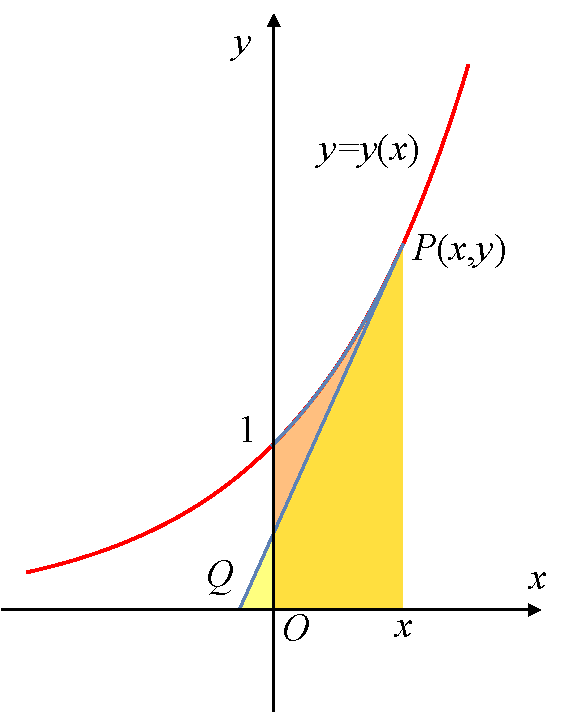
\includegraphics[width=\textwidth]{./images/ch7/eX.pdf}
			\end{center}
		\end{column}
	\end{columns}
\end{frame}

\begin{frame}
	\linespread{1.5}	
	\small 解:\it
	设所求曲线为$y=y(x)$,过其上任一点$P(x,y)\;(x\geq 0)$的切线为
	$$Y=y+y'(X-x),$$
	与$x$轴相交于$Q(x-x/y',0)$。由于$y'>0$,故当$x\geq 0$时,恒有$y\geq 1$,故
	$$S_1=\df12y\left[x-\left(x-\df{y}{y'}\right)\right]=\df{y^2}{2y'}.$$
	又
	$$S_2=\dint_0^xy(t)\d t,$$
	由已知$2S_1-S_2=1$,也即
	$$\df{y^2}{y'}-\dint_0^xy(t)\d t=1.$$
\end{frame}

\begin{frame}
	\linespread{1.5}	
	\small \it
	$$\df{y^2}{y'}-\dint_0^xy(t)\d t=1.$$
	
	对该方程两边连求导,并取$x=0$可得
	$$\left\{\begin{array}{l}
	yy''=(y')^2\\
	y(0)=1\\
	y'(0)=1
	\end{array}\right.$$
	解之得$y=e^x$,即为所求。
	\fin
\end{frame}

\section{7.4 二阶线性微分方程}

\begin{frame}
	\linespread{1.5}
	\ba{1.求解下列微分方程:(1)$y''-y=e^x+\cos x$}
	
	\bigskip
	
	\small 解:\it
	该方程的特征方程为$r^2-1=0$,特征根为$r=\pm1$,
	故其对应的齐次方程的通解为$y=C_1e^x+C_2e^{-x},(C_1,C_2\in\mbb{R})$。
	
	利用叠加原理,可以设原方程的特解为
	$$y^*=Axe^x+(B\cos x+C\sin x),$$
	带入原方程可得
	$$2Ae^x-2B\cos x-2C\sin x=e^x+\cos x,$$
	从而可得$A=\frac12,B=-\frac12,C=0$。
	综上,原方程的通解为
	$$y=C_1e^x+C_2e^{-x}+\df12xe^x-\df12\cos x,\quad (C_1,C_2\in\mbb{R})$$
\end{frame}

\begin{frame}
	\linespread{1.5}
	\ba{(2)$y^{(4)}+y''=1$}
	
	\bigskip
	
	\small 解:\it
	令$z=y''$,则原方程可化为
	$$z''+z=1,$$
	求解该方程可得其通解为$z=C_1\cos x+C_2\sin x+1,(C_1,C_2\in\mbb{R})$,
	也即
	$$y''=C_1\cos x+C_2\sin x+1,$$
	对其两边连续两次积分可得
	$$y=C_3\cos x+C_4\sin x+\df12x^2+C_5x+C_6,\quad (C_3,C_4,C_5,C_6\in\mbb{R}),$$
	即为原方程的通解。\fin
\end{frame}

\begin{frame}
	\linespread{1.5}
	\ba{2.求级数$\sumn[0]\df{x^{2n}}{(2n)!}$的和函数。 }
	
	\bigskip
	
	\small 解:\it
	该级数的收敛域为$(-\infty,+\infty)$,设其和函数为$S(x)$,则
	$$S''(x)=S(x).$$
	这是一个二阶常系数齐次线性微分方程,解之可得
	$$S(x)=C_1e^x+C_2e^{-x},\quad(C_1,C_2\in\mbb{R}).$$
	注意到$S(0)=1,S'(0)=0$,带入以上的通解,可得$C_1=C_2=\frac12$,故
	$$\sumn[0]\df{x^{2n}}{(2n)!}=\df{e^x+e^{-x}}2,\quad(x\in\mbb{R}).$$
	\fin
\end{frame}

\begin{frame}
	\linespread{1.5}
	\ba{3.设$\varphi'(x)=e^x+\sqrt x\dint_0^{\sqrt x}\varphi(\sqrt x u)\d u,$
	$\varphi(0)=0$,求$\varphi(x)$。}
	
	\bigskip
	
	\small 解:\it
	令$t=\sqrt xu$,则已知方程即为
	$$\varphi'(x)=e^x+\dint_0^x\varphi(t)\d t,$$
	对其两边关于$x$求导,结合已知条件,可得到初值问题
	$$
		\left\{\begin{array}{l}
			\varphi''(x)-\varphi(x)=e^x,\\
			\varphi(0)=0,\\
			\varphi(0)=1.
		\end{array}\right.
	$$
	解之可得
	$$\varphi(x)=\df14e^x-\df14e^{-x}+\df12xe^x.$$
	\fin
\end{frame}

\begin{frame}
	\linespread{1.5}
	\ba{4.设$y(x)$在$\mathbb{R}$上具有二阶连续导数,$y'\ne 0$,$x=x(y)$
	  为其反函数。
	    \begin{enumerate}[(1)]
% 	      \setlength{\itemindent}{1cm}
	      \item 试将$x=x(y)$所满足的微分方程
	      $$\df{\d^2x}{\d y^2}+(y+\sin x)\left(\df{\d x}{\d y}\right)^3=0$$
	      变换为$y=y(x)$所满足的微分方程;%\hfill$y''-y=-\sin x$
	      \item 求变换后的微分方程满足初始条件$y(0)=0$和$y'(0)=1.5$的解。
	    \end{enumerate}}
	
% 	\bigskip
	
% 	\small 解:\it
% 	设$m(t)$为自2000年起第$t$年时湖内的污染物总量,则
% 	$$m'=\df{m_0}6-\df{m}3,$$
% 	且$m(0)=5m_0$。
\end{frame}

\begin{frame}
	\linespread{1.5}
	\small 解:\it
	$$\df{\d^2x}{\d y^2}=\df{\d x'}{\d y}
	=\df{\d(1/y')}{\d y}=
	\df{\df{\d\frac1{y'}}{\d x}}{\df{\d y}{\d x}}=-\df{y''}{(y')^3},$$
	从而原方程可化为$y''-y=\sin x$。
	以上方程对应的齐次方程的通解为$y=C_1e^x+C_2e^{-x},(C_1,C_2\in\mbb{R})$。
	设原方程的特解为$y^*=A\cos x+B\sin x$,带入方程可解得
	$A=0,B=-\frac12$,故原方程的通解为
	$$y=C_1e^x+C_2e^{-x}-\df12\sin x,\quad (C_1,C_2\in\mbb{R}).$$
	带入初始条件,可得$C_1=-C_2=1$,故所求特解为
	$$y=e^x-e^{-x}-\df12\sin x.$$
	\fin
\end{frame}

\begin{frame}
	\linespread{1.5}
	\ba{5.设以质量为$m$的质点作直线运动。从速度等于零的时刻起,有一个与其运动方向
	一致、大小与时间成正比(比例系数为$a$)的力作用于它,与此同时地面对其的阻力
	大小与其速度成正比(比例系数为$b$),求该质点的位移函数$S(t)$(设初始位移$S(0)=0$)}
	
	\small 解:\it
	由已知
	$$S''(t)=\df{at}m-\df{bS'(t)}m.$$
	该方程对应的齐次方程的通解为$S(t)=C_1+C_2e^{-\frac{bt}m},(C_1,C_2\in\mbb{R})$。
	
	设该方程的特解为$S^*(t)=(At+B)t$,带入方程可得
	$$2A+\df bm(2At+B)=\df{at}m,$$
	由此解得$A=\df{a}{2b},B=-\df{ma}{b^2}$。
\end{frame}

\begin{frame}
	\linespread{1.5}
	
	\small \it
	
	综上原方程的通解为
	$$S(t)=C_1+C_2e^{-\frac{bt}m}+\df{at^2}{2b}-\df{mat}{b^2},
	\quad (C_1,C_2\in\mbb{R})$$
	
	又$S(0)=S'(0)=0$,带入通解中可得$C_1=\frac{m^2a}{b^3},C_2=-\frac{m^2a}{b^3}$,
	进而所求位移函数为
	$$S(x)=\frac{m^2a}{b^3}\left(1-e^{-\frac{bt}m}\right)
	+\df{at^2}{2b}-\df{mat}{b^2}.$$
	\fin
\end{frame}

% \begin{frame}{出现的问题}
% 	\linespread{1.5}
% 	  \begin{itemize}%[<+-|alert@+>]
% 	    \item 作业进度慢!
% 	    \item 概念问题
% 	    \begin{itemize}
% 	      \item \b\it 幂级数展开不熟练
% 	      \item \b\it Maclaurin级数和关于$(x-x_0)$的幂级数分不清
% 	    \end{itemize}
% 	    \item 过程不规范或不完整
% 	    \begin{itemize}
% 	      \item \b\it 求收敛域要单独讨论端点的敛散性
% 	      \item \b\it 相同幂次的项要合并,并按幂次从小到大排列
% 	      \item \b\it 书写潦草随意\pause
% 	    \end{itemize}
% 	    \item \ba{雷同!!!}
% 	  \end{itemize}
% \end{frame}

% \begin{frame}
% 	\linespread{1.5}
% 	\ba{3.设$D$是由曲线$y=\sin x+1$与三条直线$x=0,x=\pi,y=0$
% 	所围成的曲边梯形,求$D$绕$x$轴旋转一周所围成的旋转体的体积。
% 	}
% 	\pause
% 	
% % 	\bigskip
% 	
% 	\begin{columns}
% 		\begin{column}{.5\textwidth}
% 			\begin{center}
% 				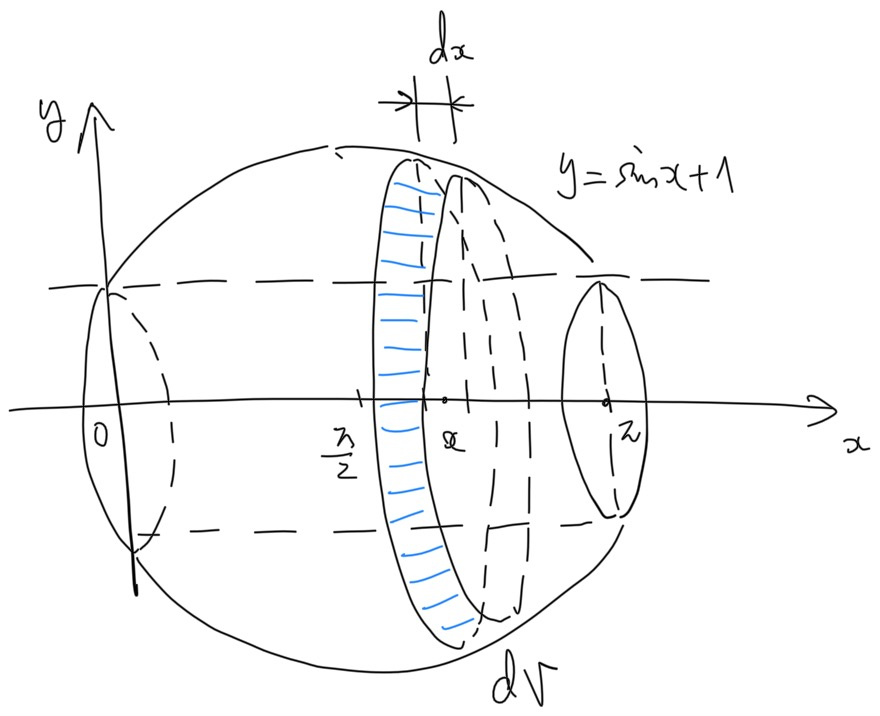
\includegraphics[width=.9\textwidth]{./images/ch6/sinx1cs.jpg}
% 		% 		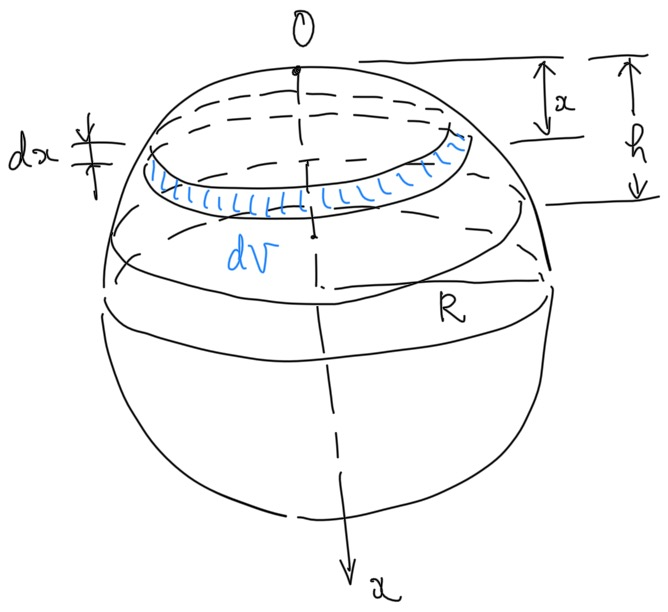
\includegraphics[width=6cm]{./images/ch6/topSp.jpg}
% 			\end{center}		
% 		\end{column}
% 		\begin{column}{.5\textwidth}
% 			\small 解:\it
% 			如图,体积微元$\d V=\pi y^2\d x$,	故所求体积
% 			$$
% 				V=\dint_0^{\pi}\pi(\sin x+1)^2\d x=\df32\pi^2.
% 			$$
% 		\end{column}
% 	\end{columns}
% \end{frame}

% % !Mode:: "TeX:UTF-8"

\titlepage

\begin{frame}{说在前面}
	\linespread{1.5}
	  \begin{itemize}[<+-|alert@+>]
	    \item \ba{箭头!箭头!箭头!}
	    \item \ba{画图!画图!画图!}
	    \item 不记得自己哪周交作业
	  \end{itemize}
\end{frame}

% \begin{frame}{需要注意的问题}
% 	\linespread{1.5}
% 	  \begin{itemize}%[<+-|alert@+>]
% 	    \item L'Hospital法则
% 	    \begin{itemize}
% 	      \item \it 只能应用于“$\df{\bm{0}}{\bm{0}}$”
% 	      和“$\df{\bm{\infty}}{\bm{\infty}}$”型
% 	      \item \it 及时使用无穷小代换进行简化
% 	      \item \it 不正规的符号:\b 
% 	      $\xlongequal{\footnotesize\mbox{“L”}}$、
% 	      $\xlongrightarrow{\footnotesize\mbox{“L'Hospital法则”}}$、
% 	      $\df{\bm{0}}{\bm{0}}$、$\df{\bm{\infty}}{\bm{\infty}}$
% 	    \end{itemize}
% 	    \item Taylor公式
% 	    \begin{itemize}
% 	      \item \it Taylor多项式不包含余项
% 	      \item \it 合并同次幂的系数
% 	      \item \it 尽量按照幂次由低到高排列,最后写余项
% 	    \end{itemize}
% 	  \end{itemize}
% \end{frame}

\section{作业讲评:8.1 向量及其运算}

\begin{frame}
	\linespread{1.5}
	\ba{1.已知$(\bm{a}\times\bm{b})\cdot\bm{c}=2$,证明:
	$$[(\bm{a}+\bm{b})\times(\bm{b}+\bm{c})]\cdot(\bm{c}+\bm{a})=4$$.}
	
	\bigskip
	
	\small 解:\it
	略!
	
	\alert{注意叉乘满足反交换律!}
\end{frame}

\begin{frame}
	\linespread{1.5}
	\ba{2.求向量$\bm{a}=(4,3,4)$在向量$\bm{b}=(2,-2,1)$上的投影长度
	及投影向量。}
	
% 	\bigskip
	
	\small 解:\it
	$\bm{a}$在$\bm{b}$上的投影长度为
	$$(\bm{a})_{\bm{b}}=\df{\bm{a}\cdot\bm{b}}{|\bm{b}|}
	=2.$$
	$\bm{b}$对应的单位向量为
	$$\bm{e}_{\bm{b}}=\df{\bm{b}}{|\bm{b}|}=\left(\df23,-\df23,\df13\right),$$
	于是$\bm{a}$在$\bm{b}$上的投影向量为
	$$(\bm{a})_{\bm{b}}\cdot\bm{e}_{\bm{b}}=\left(\df43,-\df43,\df23\right).$$
	\fin
\end{frame}

\begin{frame}
	\linespread{1.5}
	\ba{3.设$\bm{a},\bm{b}$均为非零向量,且$|\bm{b}|=1$,二者夹角为$\pi/3$,求
	$\limx{0}\df{|\bm{a}+x\bm{b}|-|\bm{a}|}{x}$。}
	
	\bigskip
	
	\small 解:\it
	\begin{align*}
		&\limx{0}\df{|\bm{a}+x\bm{b}|-|\bm{a}|}{x}
		=\limx{0}\df{|\bm{a}+x\bm{b}|^2-|\bm{a}|^2}{x(|\bm{a}+x\bm{b}|+|\bm{a}|)}\\
		&=\limx{0}\df{(\bm{a}+x\bm{b})\cdot(\bm{a}+x\bm{b})
		-\bm{a}\cdot\bm{a}}{2x|\bm{a}|}
		=\limx{0}\df{2x\bm{a}\cdot\bm{b}+x^2|\bm{b}|^2}{2x|\bm{a}|}\\
		&=\df{\bm{a}\cdot\bm{b}}{|\bm{a}|}=|\bm{b}|\cos\df{\pi}3=\df12
	\end{align*}
	\fin
	
	\ba{注意:1、$\bm{a}$和$\bm{b}$未必是二维向量,不可以简单地假设其分量形式!
	2、没有$\bm{a}^2$这种形式!}
\end{frame}

\begin{frame}
	\linespread{1.5}
	\ba{4.已知平行四边形的两对角线向量分别为$\bm{A}=\bm{m}+2\bm{n}$,
	$\bm{B}=2\bm{m}-4\bm{n}$,其中$|\bm{m}|=1,|\bm{n}|=2$,
	$\bm{m}$和$\bm{n}$的夹角为$\pi/6$,求该平行四边形的面积。}
	
	\bigskip
	
	\small 解:\it
	以$\bm{A}$和$\bm{B}$为对角线的平行四边形面积,等于以$\bm{A}$和$\bm{B}$
	为相邻边的平行四边形面积的一半,故所求面积
	\begin{align*}
		S&=\df12{|\bm{A}\times\bm{B}|}
		=\df12|(\bm{m}+2\bm{n})\times(2\bm{m}-4\bm{n})|\\
		&=\df12|-6\bm{m}\times\bm{n}|
		=3|\bm{m}||\bm{n}|\sin\df{\pi}6=3.
	\end{align*}
	\fin
	
	\ba{注意:不要忘记取模!}
\end{frame}

\begin{frame}
	\linespread{1.5}
	\ba{5.画图:在空间直角坐标系中画出一个单位正立方体,然后在其表面上画出一个正六边形,
	{\it 使得六边形的每条边分别在六面体的一个面上}。}\pause
	
	\bigskip
	
	\begin{center}
		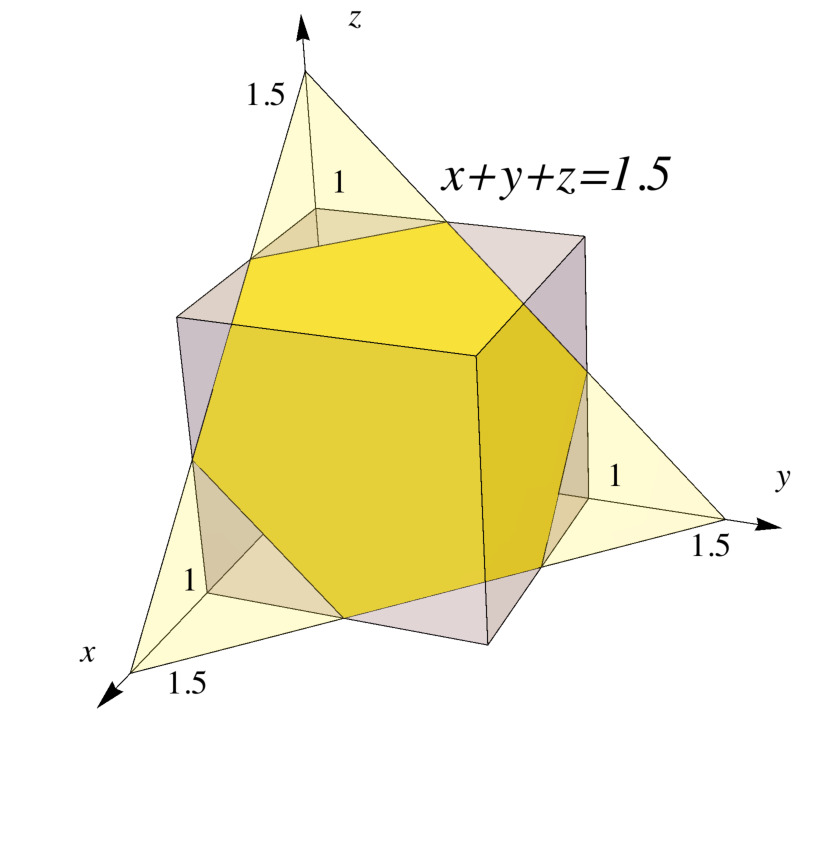
\includegraphics[width=0.5\textwidth]{./images/ch8/HexCubic.pdf}
	\end{center}
	\fin
\end{frame}

\begin{frame}
	\linespread{1.5}
	\ba{6.设向量$\bm{a},\bm{b},\bm{c}$不共面,向量
	$\bm{d}=\alpha\bm{a}+\beta\bm{b}+\gamma\bm{c}$,
	如果将$\bm{a},\bm{b},\bm{c},\bm{d}$的起点都放在一起,
	参数$\alpha,\beta,\gamma$须满足什么条件,方能使其终点在同一个平面上? }
	
	\bigskip
	
	\begin{columns}
		\begin{column}{.5\textwidth}
			\begin{center}
				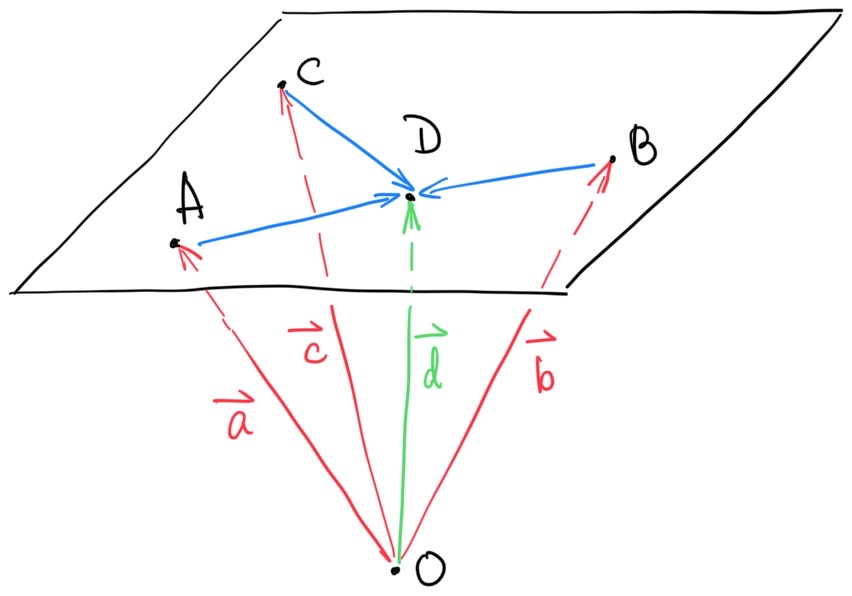
\includegraphics[width=.9\textwidth]{./images/ch8/abcd.jpg}
		% 		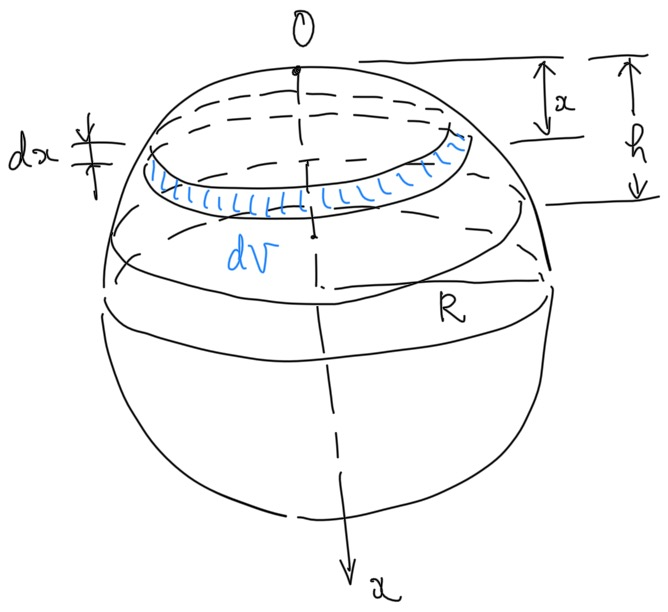
\includegraphics[width=6cm]{./images/ch6/topSp.jpg}
			\end{center}
		\end{column}
		\begin{column}{.5\textwidth}
			\small 解:\it
			由混合积的几何意义,点$A,B,C,D$共面当且仅当
			$$[(\bm{d}-\bm{a})\times(\bm{d}-\bm{b})]\cdot(\bm{d}-\bm{c})=0,$$
			利用向量运算的性质化简,最后可得$\alpha+\beta+\gamma=1$。\fin
		\end{column}
	\end{columns}
\end{frame}

\section{补充例题}

\begin{frame}{判断}
	\linespread{1.2}
	\begin{enumerate}
	  \item $\bm{a}\cdot\bm{a}\cdot\bm{a}=\bm{a}^3$\quad\pause\ba{$\times$}\pause
	  \item $\bm{a}\ne 0$时,$\df{\bm{a}}{\bm{a}}=1$\quad\pause\ba{$\times$}\pause
	  \item $\bm{a}(\bm{a}\cdot\bm{b})=\bm{a}^2\bm{b}$
	    \quad\pause\ba{$\times$}\pause
	  \item $(\bm{a}\cdot\bm{b})^2=\bm{a}^2\bm{b}^2$\quad\pause\ba{$\times$}\pause
	  \item $|\bm{a}\cdot\bm{b}|=|\bm{a}|\cdot|\bm{b}|$
		\quad\pause\ba{$\times$}\pause
	  \item $(\bm{a}+\bm{b})\times(\bm{a}-\bm{b})=\bm{a}\times\bm{a}
  		-\bm{b}\times\bm{b}=0$
  		\quad\pause\ba{$\times$}\pause
  	  \item $\bm{a}\ne 0$时,$\bm{a}\cdot\bm{b}
  	  	=\bm{a}\cdot\bm{c}\Rightarrow\bm{b}=\bm{c}$
  	  	\quad\pause\ba{$\times$}\pause
  	  \item  $\bm{a}\ne 0$时,$\bm{a}\times\bm{b}
  	  	=\bm{a}\times\bm{c}\Rightarrow\bm{b}=\bm{c}$
  	  	\quad\pause\ba{$\times$}
	\end{enumerate}
\end{frame}

\begin{frame}{填空}
	\linespread{1.2}
	
	\ba{1.}\;设$\bm{a},\bm{b}$均为非零向量,则
	其角平分线上的向量为
	\underline{\uncover<2->{\;\b{$C\left(\df{\bm{a}}{|\bm{a}|}
	+\df{\bm{b}}{|\bm{b}|}\right),\;(C\in\mathbb{R})$}}\;}.\\[1em]
	
	\ba{2.}\;设$\bm{a},\bm{b},\bm{c}$均为非零向量,且$\bm{a}=\bm{b}\times\bm{c}$,
	$\bm{b}=\bm{c}\times\bm{a}$,
	$\bm{c}=\bm{a}\times\bm{b}$则
	$|\bm{a}|+|\bm{b}|+|\bm{c}|=$
	\underline{\uncover<3->{\;\b{$3$}}\;}.\\[1em]

	\ba{3.}\;设$|\bm{a}|=2,|\bm{b}|=2$,$\bm{a}$和$\bm{b}$
	的夹角为$\pi/3$,则$|2\bm{a}-3\bm{b}|=$
	\underline{\uncover<4->{\;\b{$2\sqrt7$}}\;}.\\[1em]
		
	\ba{4.}\;平面$Ax+By+Cz+D_i=0\;(i=1,2)$之间的距离为
	\underline{\uncover<5->{\;\b{$\df{|D_1-D_2|}{\sqrt{A^2+B^2+C^2}}$}}\;}.
\end{frame}

\begin{frame}{选择}
	\linespread{1.3}
	\ba{1.}\;设$\bm{a},\bm{b},\bm{c}$均为非零向量,则与$\bm{a}$不垂直的是
	(\underline{\uncover<2->{\;\b{D}}\;})
	\begin{enumerate}[(A)]
	  \item $(\bm{a}\cdot\bm{c})\bm{b}-(\bm{a}\cdot\bm{b})\bm{c}$
	  \item $\bm{b}-\left(\df{\bm{a}\cdot\bm{b}}{\bm{|a|}^2}\right)\bm{a}$
	  \item $\bm{a}\times\bm{b}$
	  \item $\bm{a}+(\bm{a}\times\bm{b})\times\bm{a}$
	\end{enumerate}
\end{frame}

\begin{frame}{选择}
	\linespread{1.3}
	\ba{2.}\;设$\bm{a},\bm{b}$为非零向量,$|\bm{a}-\bm{b}|=|\bm{a}+\bm{b}|$,则
	(\underline{\uncover<2->{\;\b{C}}\;})
	\begin{enumerate}[(A)]
	  \item $\bm{a}-\bm{b}=\bm{a}+\bm{b}$
	  \item $\bm{a}=\bm{b}$
	  \item $\bm{a}\cdot\bm{b}=0$
	  \item $\bm{a}\times\bm{b}=0$
	\end{enumerate}
\end{frame}

% \begin{frame}{选择}
% 	\linespread{1.3}
% 	\ba{3.}\;设$\bm{a},\bm{b}$为非零向量,且满足
% 	$(\bm{a}+3\bm{b})\perp(7\bm{a}-5\bm{b})$,
% 	$(\bm{a}-4\bm{b})\perp(7\bm{a}+2\bm{b})$,则
% 	向量$\bm{a}$和$\bm{b}$的夹角为
% 	(\underline{\uncover<2->{\;\b{C}}\;})
% 	\begin{enumerate}[(A)]
% 	  \item $0$
% 	  \item $\pi/2$
% 	  \item $\pi/3$
% 	  \item $2\pi/3$
% 	\end{enumerate}
% \end{frame}

\begin{frame}{选择}
	\linespread{1.3}
	\ba{3.}\;设平面$\pi$位于平面$x-2y+z-2=0$和$x-2y+z-6=0$之间,
	且与此二平面的距离之比为$1:3$,则$\pi$的方程为
	(\underline{\uncover<2->{\;\b{A}}\;})
	\begin{enumerate}[(A)]
	  \item $x-2y+z-5=0$或$x-2y+z-3=0$
	  \item $x-2y+z+8=0$
	  \item $x+2y+4z=0$
	  \item $x-2y+5z-3=0$
	\end{enumerate}
\end{frame}

\begin{frame}{选择}
	\linespread{1.3}
	\ba{4.}\;设$\left|\begin{array}{ccc}
	a_1 & b_1 & c_1\\ a_2 & b_2 & c_2\\ a_3 & b_3 & c_3
	\end{array}\right|\ne 0$,则
	直线
	$\df{x-a_3}{a_1-a_2}=\df{y-b_3}{b_1-b_2}$
	$=\df{z-c_3}{c_1-c_2}$
	和
	$\df{x-a_1}{a_2-a_3}=\df{y-b_1}{b_2-b_3}=\df{z-c_1}{c_2-c_3}$
	(\underline{\uncover<2->{\;\b{A}}\;})
	\begin{enumerate}[(A)]
	  \item 相交于一点
	  \item 重合
	  \item 平行但不重合
	  \item 异面直线
	\end{enumerate}
\end{frame}

\begin{frame}{解答}
	\linespread{1.2}
	\ba{1.}\;过原点且与
	$$\left\{\begin{array}{l}
	x=1\\ y=-1+t\\ z=2+t
	\end{array}\right.$$
	和$x+1=\df{y+2}2=z-1$都平行的平面方程。
	
	\pause\alert{提示:}\it\b  
	$$x-y+z=0$$
\end{frame}

\begin{frame}{解答}
	\linespread{1.2}
	\ba{2.}\;求过点$M(3,1,-2)$和直线$\df{x-4}5=\df{y+3}2=\df z1$
	的平面方程。
	
	\pause\ba{法一:}\it\b  
	$\bm{n}=\bm{s}\times\bm{MM_1}=(-8,9,22)$,平面方程
	$$8x-9y-22x-59=0$$
	
	\pause\ba{法二:}
	直线的一般式方程:$\left\{\begin{array}{l}x-5y-4=0\\ 
	y-2z+3=0\end{array}\right.$,建立平面束方程,进而可得$\lambda=8,\mu=-9$
\end{frame}

% \begin{frame}
% 	\linespread{1.2}
% 	\ba{3.}\;过直线
% 	$\df{x-1}2=\df{y+2}{-3}=\df{z-2}2$且垂直于平面
% 	$3x+2y-z=5$的平面方程。
% 	
% 	\pause\alert{提示:}{\b  
% 	$$x-8y-13z+9=0$$}
% 	
% 	\pause
% 	\ba{4.}\;求过直线
% 	$$\left\{\begin{array}{l}
% 		x+5y+z=0\\
% 		x-z+4=0
% 	\end{array}\right.$$
% 	且与平面$\pi:x-4y-8z+12=0$的夹角为$\pi/4$的平面方程。
% \end{frame}

\begin{frame}
	\linespread{1.2}
	\ba{3.}\;过点$(-1,0,4)$,平行于平面
	$3x-4y+z=10$,且与直线$x+1=y-3=\df z2$
	相交的直线方程。

	\pause\alert{提示:}\it\b 建立所求直线的参数方程,最终解得
	$$\df{x+1}{16}=\df{y}{19}=\df{z-4}{28}$$
\end{frame}

\begin{frame}
	\linespread{1.2}
	\ba{4.}\;已知$P(3,1,-4)$和$L:\df{x+1}2=\df{y-4}{-2}=z-1$,求
	\begin{enumerate}
	  \item $P$到$L$的距离;
	  \item $P$在$L$上的垂足$Q$的坐标;
	  \item 设$R(1,2,3)$在$L$上的垂足为$N$,求$QN$的长度。
	\end{enumerate}

	\pause\alert{提示:}\it\b
	$(1)\sqrt{41}$\quad$(2)(1,2,2)$\quad$(3)\df13$
\end{frame}

\begin{frame}
	\linespread{1.2}
	\ba{5.}\;已知直线
	$$L_1:\left\{\begin{array}{l}
		x+y+z+1=0\\
		2x-y+3z+4=0
	\end{array}\right.
	\quad
	L_2:\left\{\begin{array}{l}
		x=-1+2t\\
		y=-t\quad(t\in\mathbb{R})\\
		z=2-2t
	\end{array}\right.
	$$
	\begin{enumerate}[(1)]
% 	  \setlength{\itemindent}{1cm}
	  \item 证明两直线异面;
	  \item 求两直线间的距离;
	  \item 求二者的公垂线方程。
	\end{enumerate}
	
	\pause\alert{提示:}\it\b
	$L_1,L_2$的标准式方程
	$$\df{x+3}4=\df{y-1}{-1}=\df{z-1}{-3},\quad
	\df{x+1}2=\df y{-1}=\df{z-2}{-2}$$
\end{frame}

% \begin{frame}
% 	\linespread{1.2}
% 	\ba{8.}\;计算由以下平面所围成的立体体积:
% 	$$a_ix+b_iy+c_iz=\pm h_i,\;i=1,2,3,$$
% 	其中:$a_i,b_i,c_i$为常数,$h_i\ne0(i=1,2,3)$,且
% 	$$\Delta=\left|\begin{array}{ccc}
% 	a_1 & b_1 & c_1\\ a_2 & b_2 & c_2 \\ a_3 & b_3 & c_3
% 	\end{array}\right|\ne 0$$
% 	
% 	\pause\alert{提示:}\b
% 	$$\left[(\bm{s}_1\times\bm{s}_2)\times
% 	(\bm{s}_2\times\bm{s}_3)\right]\cdot(\bm{s}_3\times\bm{s}_1)=
% 	\left[(\bm{s}_1\times\bm{s}_2)\cdot\bm{s}_3\right]^2$$ 
% \end{frame}
% 
% \begin{frame}{讨论}
% 	\linespread{1.2}
% 	\begin{enumerate}
% 	  \item 证明:$\bm{s}_1\times(\bm{s}_2\times\bm{s}_3)
% 	  	=(\bm{s}_1\cdot\bm{s}_3)\bm{s}_2
% 		-(\bm{s}_1\cdot\bm{s}_2)\bm{s}_3$\pause
% 	  \item 证明:$\left[(\bm{s}_1\times\bm{s}_2)\times
% 	  	(\bm{s}_2\times\bm{s}_3)\right]
% 		\cdot(\bm{s}_3\times\bm{s}_1)
% 		=\left[(\bm{s}_1\times\bm{s}_2)\cdot\bm{s}_3\right]^2$\pause
% 	  \item $\bm{s}_1\times(\bm{s}_2\times\bm{s}_3)
% 	  =(\bm{s}_1\times\bm{s}_2)\times\bm{s}_3$成立吗?
% 	\end{enumerate}
% 	\ba{提示:}\it\b 反例:
% 	$$\bm{j}\times(\bm{i}\times\bm{i})=0$$
% 	$$(\bm{j}\times\bm{i})\times\bm{i}=-\bm{k}\times\bm{i}=-\bm{j}$$
% \end{frame}

% \begin{frame}{出现的问题}
% 	\linespread{1.5}
% 	  \begin{itemize}%[<+-|alert@+>]
% 	    \item 作业进度慢!
% 	    \item 概念问题
% 	    \begin{itemize}
% 	      \item \b\it 幂级数展开不熟练
% 	      \item \b\it Maclaurin级数和关于$(x-x_0)$的幂级数分不清
% 	    \end{itemize}
% 	    \item 过程不规范或不完整
% 	    \begin{itemize}
% 	      \item \b\it 求收敛域要单独讨论端点的敛散性
% 	      \item \b\it 相同幂次的项要合并,并按幂次从小到大排列
% 	      \item \b\it 书写潦草随意\pause
% 	    \end{itemize}
% 	    \item \ba{雷同!!!}
% 	  \end{itemize}
% \end{frame}

% \begin{frame}
% 	\linespread{1.5}
% 	\ba{3.设$D$是由曲线$y=\sin x+1$与三条直线$x=0,x=\pi,y=0$
% 	所围成的曲边梯形,求$D$绕$x$轴旋转一周所围成的旋转体的体积。
% 	}
% 	\pause
% 	
% % 	\bigskip
% 	
% 	\begin{columns}
% 		\begin{column}{.5\textwidth}
% 			\begin{center}
% 				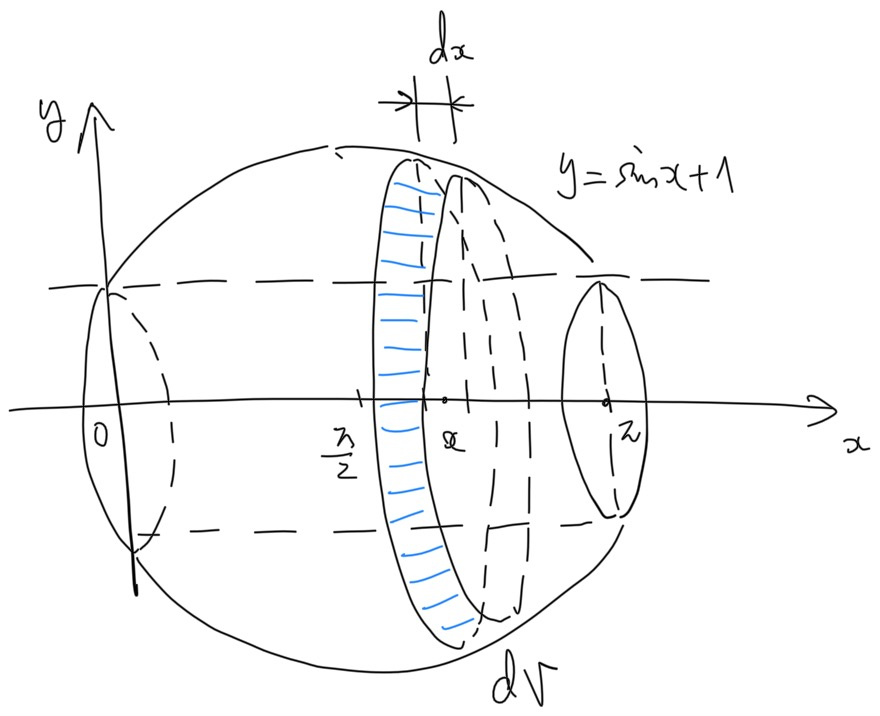
\includegraphics[width=.9\textwidth]{./images/ch6/sinx1cs.jpg}
% 		% 		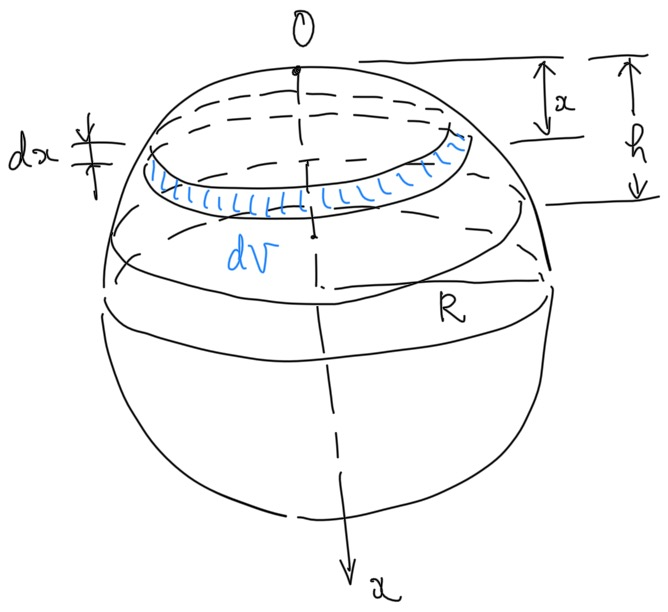
\includegraphics[width=6cm]{./images/ch6/topSp.jpg}
% 			\end{center}		
% 		\end{column}
% 		\begin{column}{.5\textwidth}
% 			\small 解:\it
% 			如图,体积微元$\d V=\pi y^2\d x$,	故所求体积
% 			$$
% 				V=\dint_0^{\pi}\pi(\sin x+1)^2\d x=\df32\pi^2.
% 			$$
% 		\end{column}
% 	\end{columns}
% \end{frame}

% % !Mode:: "TeX:UTF-8"

\titlepage

% \begin{frame}{说在前面}
% 	\linespread{1.5}
% 	  \begin{itemize}[<+-|alert@+>]
% 	    \item \ba{箭头!箭头!箭头!}
% 	    \item \ba{画图!画图!画图!}
% 	    \item 不记得自己哪周交作业
% 	  \end{itemize}
% \end{frame}

% \begin{frame}{需要注意的问题}
% 	\linespread{1.5}
% 	  \begin{itemize}%[<+-|alert@+>]
% 	    \item L'Hospital法则
% 	    \begin{itemize}
% 	      \item \it 只能应用于“$\df{\bm{0}}{\bm{0}}$”
% 	      和“$\df{\bm{\infty}}{\bm{\infty}}$”型
% 	      \item \it 及时使用无穷小代换进行简化
% 	      \item \it 不正规的符号:\b 
% 	      $\xlongequal{\footnotesize\mbox{“L”}}$、
% 	      $\xlongrightarrow{\footnotesize\mbox{“L'Hospital法则”}}$、
% 	      $\df{\bm{0}}{\bm{0}}$、$\df{\bm{\infty}}{\bm{\infty}}$
% 	    \end{itemize}
% 	    \item Taylor公式
% 	    \begin{itemize}
% 	      \item \it Taylor多项式不包含余项
% 	      \item \it 合并同次幂的系数
% 	      \item \it 尽量按照幂次由低到高排列,最后写余项
% 	    \end{itemize}
% 	  \end{itemize}
% \end{frame}

\begin{frame}
	\linespread{1.5}
	\ba{1.求过直线$x=y=z$,且垂直于$xOy$坐标面的平面的一般式方程。}
	
	\bigskip
	
	\small 解:\it
	所求平面的法向量
	$$\bm{n}=\left|\begin{array}{ccc}
		\bm{i} & \bm{j} & \bm{k}\\
		1 & 1 & 1 \\
		0 & 0 & 1
	\end{array}\right|=(1,-1,0).$$
	直线$x=y=z$过原点,故原点位于所求平面上,从而可得其方程为
	$$x-y=0.$$
	\fin
\end{frame}

\begin{frame}
	\linespread{1.5}
	\ba{2.求点$(1,3,1)$关于平面$x+y=0$的对称点。}
	
% 	\bigskip
	
	\small 解:\it
	过点$(1,3,1)$垂直于平面$x+y=0$的直线方向为
	$$\df{x-1}1=\df{y-3}1=\df{z-1}0.$$
	其于平面的交点为$(-1,1,1)$,从而所求对称点为
	$(-3,-1,1)$。\fin
\end{frame}

\begin{frame}
	\linespread{1.5}
	\ba{3.求过点$(3,1,-2)$且过直线$\df{x-4}5=\df{y+3}2=z$的平面
	的一般式方程。}
	
	\bigskip
	
	\small 解:\it
	所求平面的法向量为
	$$\bm{n}=\left|\begin{array}{ccc}
		\bm{i} & \bm{j} & \bm{k}\\
		1 & -4 & 2 \\
		5 & 2 & 1
	\end{array}\right|=(-8,9,22).$$
	从而该平面的方程为
	$$-8x+9y+22z+59=0.$$
	\fin
\end{frame}

\begin{frame}
	\linespread{1.5}
	\ba{4.求直线$\left\{\begin{array}{l}
	  	2x-y=0, \\ 3x-y-z-9=0
	  \end{array}\right.$
	  在平面$2x-y+z=1$上的投影直线的对称式方程。}
	
	\bigskip
	
	\small 解:\it
	已知直线的方向向量为
	$$\bm{s_1}=(2,-1,0)\times(3,-1,-1)=(1,2,1).$$
	过该直线且与已知平面垂直的平面的法向量为
	$$\bm{n}_1=(1,2,1)\times(2,-1,1)=(3,1,-5).$$
	于是所求直线的方向向量为
	$$\bm{s}=(3,1,-4)\times(2,-1,1)=(-4,-13,-5).$$
\end{frame}


\begin{frame}
	\linespread{1.5}
	\ba{4.求直线$\left\{\begin{array}{l}
	  	2x-y=0, \\ 3x-y-z-9=0
	  \end{array}\right.$
	  在平面$2x-y+z=1$上的投影直线的对称式方程。}
	
	\bigskip
	
	\small 解续:\it
	
	又联立已知直线与已知平面的方程可解得$(x,y,z)=(10,20,1)$,于是可知所求直线的
	对称式方程为
	$$\df{x-10}{4}=\df{y-20}{13}=\df{z-1}{5}.$$
	\fin
\end{frame}


\begin{frame}
	\linespread{1.5}
	\ba{5.求过直线
	$\left\{\begin{array}{l}
		x+y=0\\
		x+z+1=0
	\end{array}\right.$
	且与平面$\pi:x-4y-8z+12=0$的夹角为$\pi/4$的平面方程。}\pause
	
	\bigskip
	
	\small 解续:\it 由已知,可设过已知直线的平面束方程为
	$$\lambda(x+y)+\mu(x+z+1)=0,$$
	即$(\lambda+\mu)x+\lambda y+\mu z+\mu=0.$
	由已知
	$$\cos\df{\pi}4=\df{(\lambda+\mu,\lambda,\mu)\cdot
	(1,-4,-8)}{|(\lambda+\mu,\lambda,\mu)||(1,-4,-8)|},$$
	化简可得
	$$72\lambda^2+39\lambda\mu+32\mu^2=0,$$
	该方程无解,从而可知所求平面不存在。
	\fin
\end{frame}

\begin{frame}
	\linespread{1.5}
	\ba{6.画出下列各平面所围立体的图形:
	
	(1)$x=0,y=0,z=0,x=2,y=2,3x+4y+6z=12$}
	
	\bigskip
	
	\begin{center}
		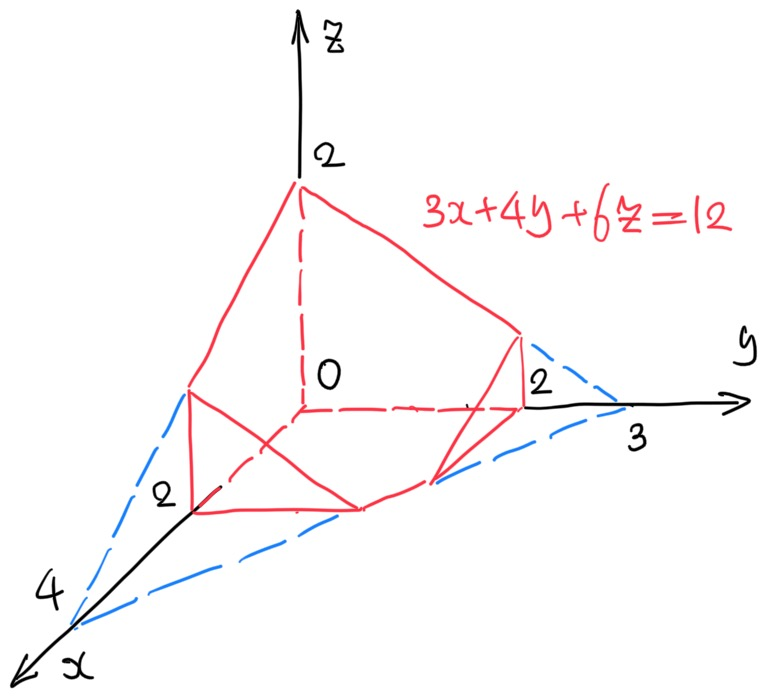
\includegraphics[width=0.6\textwidth]{./images/ch8/xyz12.jpg}
	\end{center}
\end{frame}

\begin{frame}
	\linespread{1.5}
	\ba{(2)$x+y=1,x+y+z=2,z=0,x=0,y=0$}
	
	\bigskip
	
	\begin{center}
		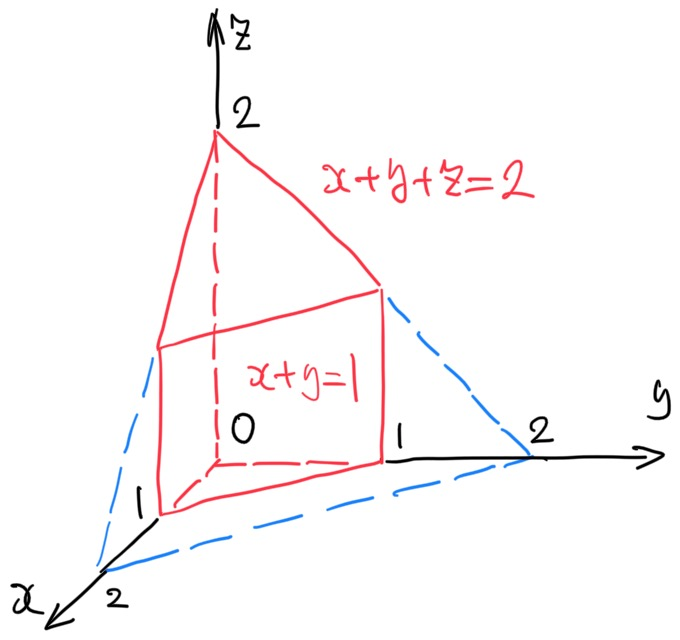
\includegraphics[width=0.6\textwidth]{./images/ch8/xyz2.jpg}
	\end{center}
\end{frame}

% \begin{frame}{出现的问题}
% 	\linespread{1.5}
% 	  \begin{itemize}%[<+-|alert@+>]
% 	    \item 作业进度慢!
% 	    \item 概念问题
% 	    \begin{itemize}
% 	      \item \b\it 幂级数展开不熟练
% 	      \item \b\it Maclaurin级数和关于$(x-x_0)$的幂级数分不清
% 	    \end{itemize}
% 	    \item 过程不规范或不完整
% 	    \begin{itemize}
% 	      \item \b\it 求收敛域要单独讨论端点的敛散性
% 	      \item \b\it 相同幂次的项要合并,并按幂次从小到大排列
% 	      \item \b\it 书写潦草随意\pause
% 	    \end{itemize}
% 	    \item \ba{雷同!!!}
% 	  \end{itemize}
% \end{frame}

% \begin{frame}
% 	\linespread{1.5}
% 	\ba{3.设$D$是由曲线$y=\sin x+1$与三条直线$x=0,x=\pi,y=0$
% 	所围成的曲边梯形,求$D$绕$x$轴旋转一周所围成的旋转体的体积。
% 	}
% 	\pause
% 	
% % 	\bigskip
% 	
% 	\begin{columns}
% 		\begin{column}{.5\textwidth}
% 			\begin{center}
% 				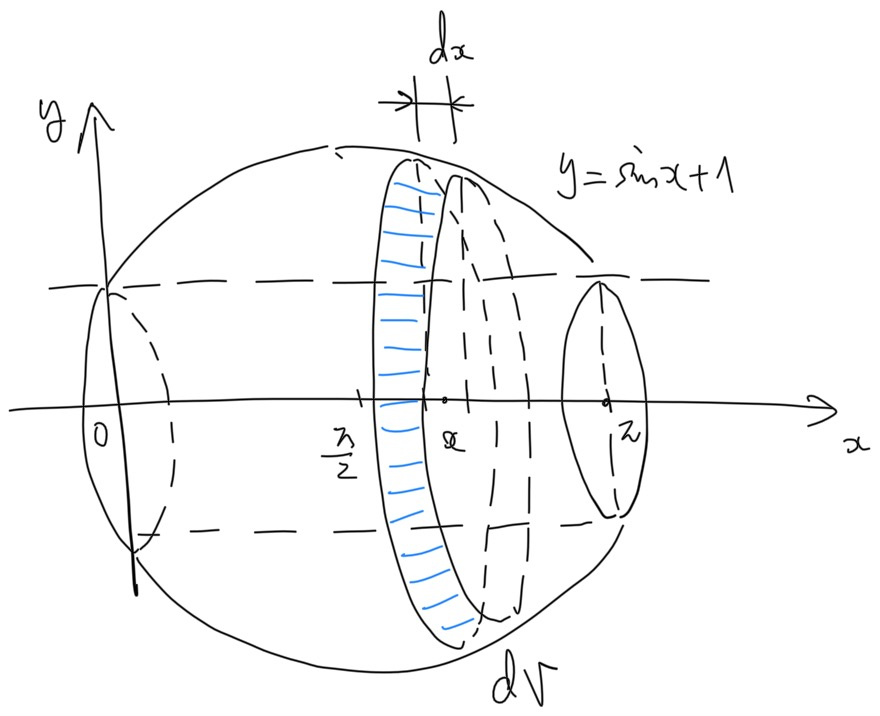
\includegraphics[width=.9\textwidth]{./images/ch6/sinx1cs.jpg}
% 		% 		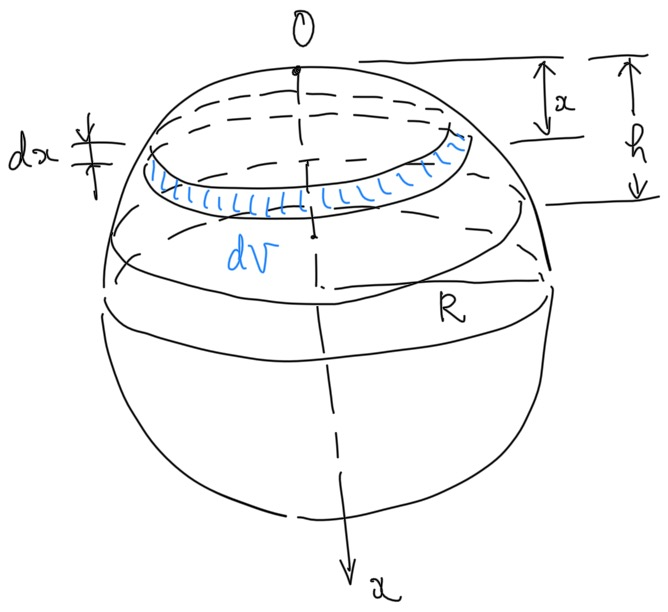
\includegraphics[width=6cm]{./images/ch6/topSp.jpg}
% 			\end{center}		
% 		\end{column}
% 		\begin{column}{.5\textwidth}
% 			\small 解:\it
% 			如图,体积微元$\d V=\pi y^2\d x$,	故所求体积
% 			$$
% 				V=\dint_0^{\pi}\pi(\sin x+1)^2\d x=\df32\pi^2.
% 			$$
% 		\end{column}
% 	\end{columns}
% \end{frame}

% % !Mode:: "TeX:UTF-8"

\titlepage

\begin{frame}{说在前面}
	\linespread{1.5}
	  \begin{itemize}[<+-|alert@+>]
	    \item \ba{箭头!箭头!箭头!}
	    \item \ba{画图!画图!画图!}
	    \item \ba{雷同!雷同!雷同!}
% 	    \item 不记得自己哪周交作业
	  \end{itemize}
\end{frame}

% \begin{frame}{需要注意的问题}
% 	\linespread{1.5}
% 	  \begin{itemize}%[<+-|alert@+>]
% 	    \item L'Hospital法则
% 	    \begin{itemize}
% 	      \item \it 只能应用于“$\df{\bm{0}}{\bm{0}}$”
% 	      和“$\df{\bm{\infty}}{\bm{\infty}}$”型
% 	      \item \it 及时使用无穷小代换进行简化
% 	      \item \it 不正规的符号:\b 
% 	      $\xlongequal{\footnotesize\mbox{“L”}}$、
% 	      $\xlongrightarrow{\footnotesize\mbox{“L'Hospital法则”}}$、
% 	      $\df{\bm{0}}{\bm{0}}$、$\df{\bm{\infty}}{\bm{\infty}}$
% 	    \end{itemize}
% 	    \item Taylor公式
% 	    \begin{itemize}
% 	      \item \it Taylor多项式不包含余项
% 	      \item \it 合并同次幂的系数
% 	      \item \it 尽量按照幂次由低到高排列,最后写余项
% 	    \end{itemize}
% 	  \end{itemize}
% \end{frame}

\section{空间曲面}

\begin{frame}
	\linespread{1.5}
	\ba{1.求直线$l:\df{x}{a}=\df{y-b}0=z$绕$z$轴旋转一周所得曲面方程,
	并指出该曲面的类型。}
	
	\bigskip
	
	\small 解:\it
	设$P(x,y,z)$为所求曲面上任意一点,则其必位于直线$l$上某点$Q$绕$z$轴旋转的轨迹上,
	$Q$的坐标可表示为$(at,b,t)$,故必有
	$$\left\{\begin{array}{l}
		x^2+y^2=(at)^2+b^2\\
		z=t
	\end{array}\right.$$
	消去以上两个方程中的$t$,可得
	$$x^2+y^2-a^2z^2=b^2.$$
	即为所求的旋转曲面方程,根据$a,b$取值的不同,其对应的几何对象分别为:
	\begin{enumerate}[(1)]
	  \setlength{\itemindent}{1cm}
	  \item $a=b=0$:$z$轴;
	  \item $a\ne0,b=0$:圆锥面;
	  \item $a\ne0,b\ne0$:单叶双曲面;
	  \item $a=0,b\ne0$:圆柱面。
	\end{enumerate}
	\fin
\end{frame}

\begin{frame}
	\linespread{1.5}
% 	\ba{1.求直线$l:\df{x}{a}=\df{y-b}0=z$绕$z$轴旋转一周所得曲面方程,
% 	并指出该曲面的类型。}
	
% 	\bigskip
	
	\small \it
	旋转曲面方程:
	$$x^2+y^2-a^2z^2=b^2.$$
	根据$a,b$取值的不同,其对应的曲面分别为:
	\begin{enumerate}[(1)]
	  \setlength{\itemindent}{1cm}
	  \item $a=b=0$:$z$轴;
	  \item $a\ne0,b=0$:圆锥面;
	  \item $a\ne0,b\ne0$:单叶双曲面;
	  \item $a=0,b\ne0$:圆柱面。
	\end{enumerate}
	\fin
\end{frame}

\begin{frame}
	\linespread{1.5}
	\ba{2.已知点$A(1,0,0)$与点$B(0,1,1)$,直线$AB$绕$z$轴旋转一周
	所成的旋转曲面为$S$,求$S$与$z=0$、$z=1$所围成的立体体积。}
	\pause

% 	\bigskip
	\small 
	\begin{columns}
		\begin{column}{.4\textwidth}
			\begin{center}
				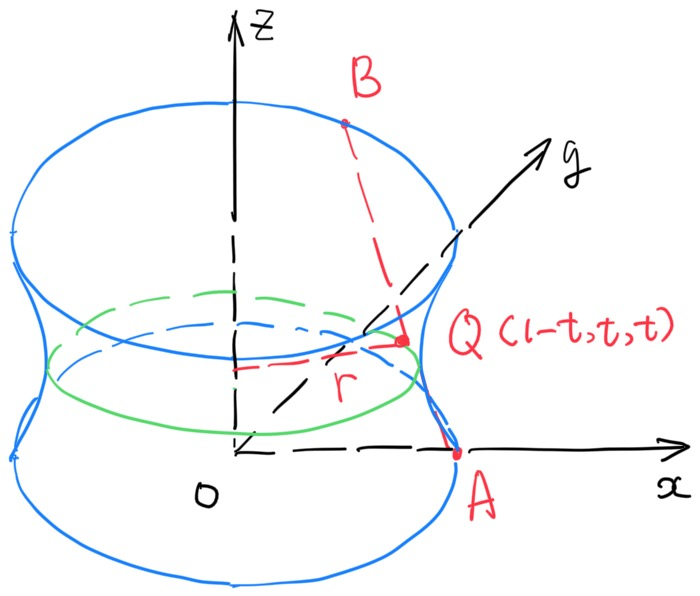
\includegraphics[width=.9\textwidth]{./images/ch8/abzz.jpg}
		% 		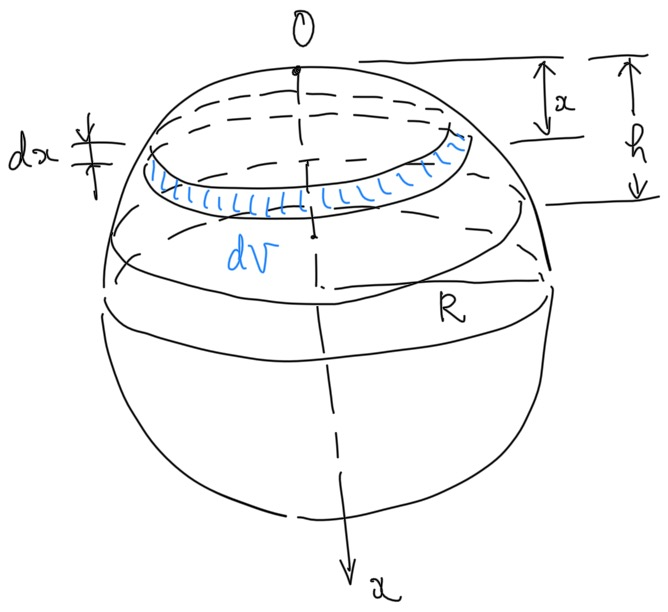
\includegraphics[width=6cm]{./images/ch6/topSp.jpg}
			\end{center}
		\end{column}
		\begin{column}{.6\textwidth}
			解:\it
			则所求立体体积为
			$$V=\dint_0^1\pi r^2\d z.$$
			其中$r$为与$z$对应的$AB$上某点$Q$到$z$轴的距离,注意到
			直线$AB$的参数方程为
			$x=1-t,\quad y=t,\quad z=t$,
			故$r=\sqrt{x^2+y^2}=\sqrt{1-2t+2t^2}$,进而
		\end{column}
	\end{columns}
	$$V=\dint_0^1\pi r^2\d z
	=\dint_0^1\pi(1-2t+2t^2)\d t=\df23\pi.$$
	\fin
\end{frame}

\begin{frame}
	\linespread{1.5}
	\ba{3.设柱面的母线平行于直线$x=y=z$,准线为$xOy$平面内的单位圆
	$x^2+y^2=1$,求柱面的方程。}
	\pause

% 	\bigskip
	\small 
	\begin{columns}
		\begin{column}{.4\textwidth}
			\begin{center}
				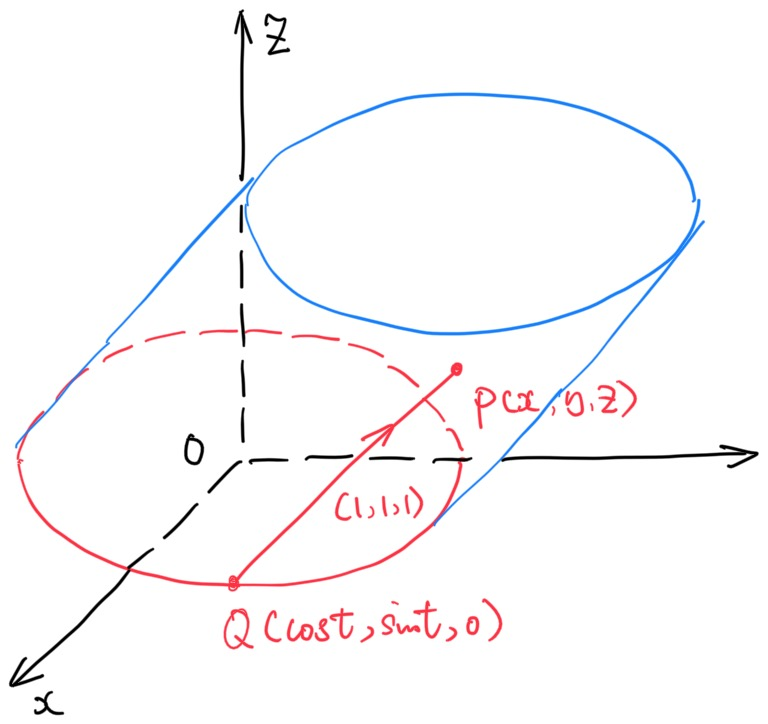
\includegraphics[width=.9\textwidth]{./images/ch8/cpq.jpg}
		% 		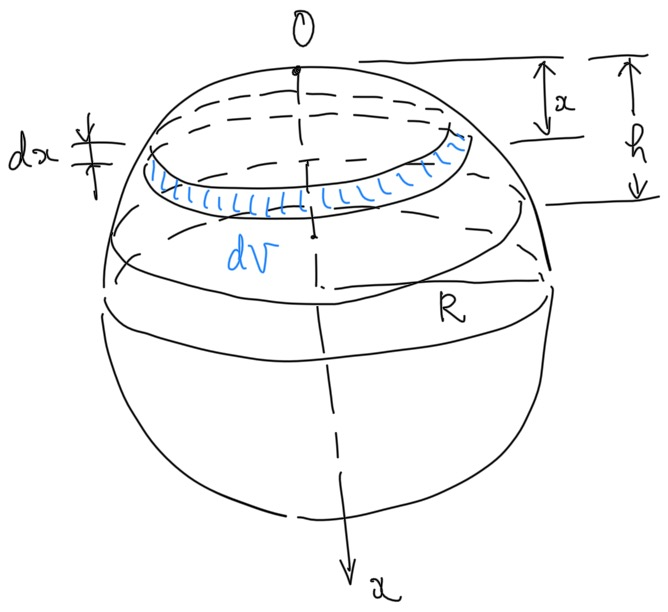
\includegraphics[width=6cm]{./images/ch6/topSp.jpg}
			\end{center}
		\end{column}
		\begin{column}{.6\textwidth}
			解:\it
			设$P(x,y,z)$为所求柱面上任意一点,由柱面的特点可知,其必位于过
			已知单位圆上某点$Q(\cos t,\sin t,0)$且方向平行于$(1,1,1)$的直线上。
			从而可得
			$$\df{x-\cos t}1=\df{y-\sin t}1=\df{z}1,$$
			消去其中的参数$t$,可得
			$$(x-z)^2+(y-z)^2=1,$$
			即为所求柱面的方程。\fin
		\end{column}
	\end{columns}
\end{frame}

\section{空间曲线}

\begin{frame}
	\linespread{1.5}
	\ba{1.一束光线垂直于平面$x+y+z=0$,照射在球面$x^2+y^2+(z-1)^2=1$上,
	求球面在$xOy$平面上的投影的边界曲线方程。}
	
% 	\bigskip
	
	\small 解:\it 如图
	\begin{center}
		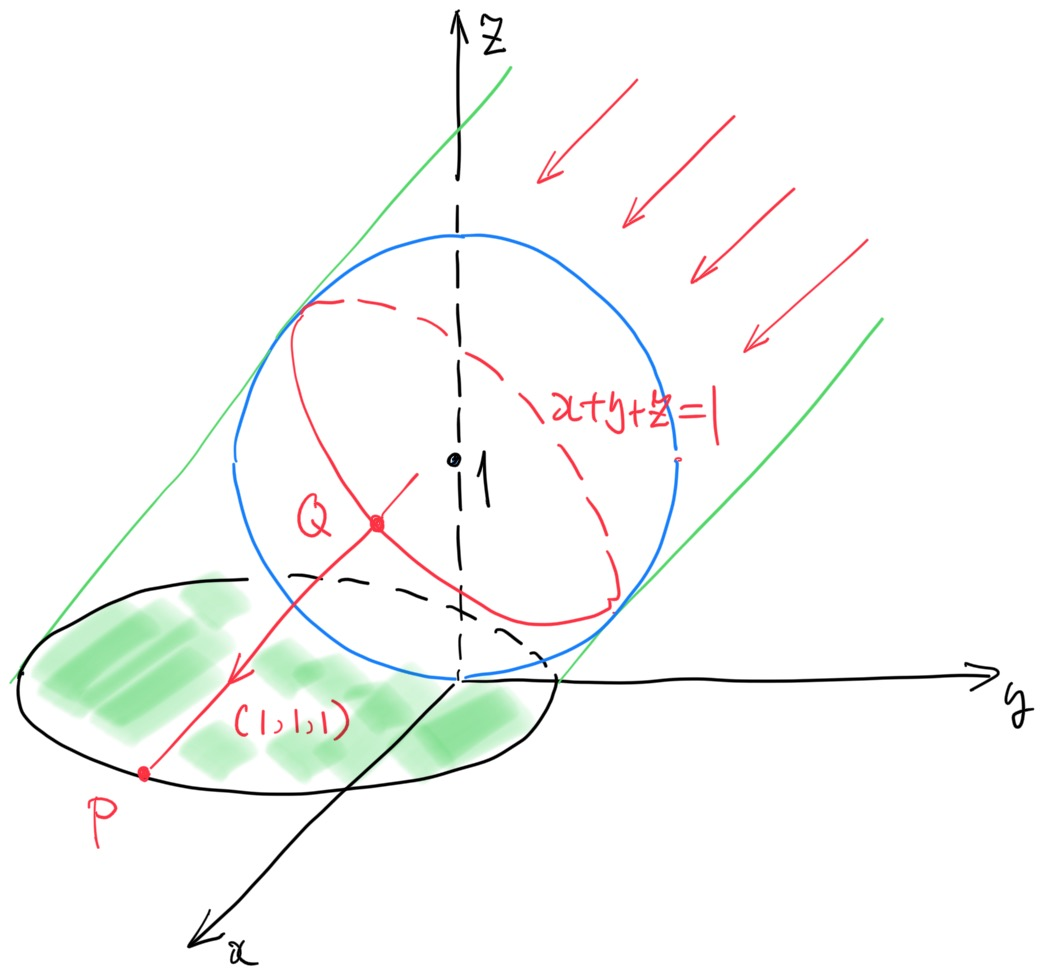
\includegraphics[width=0.5\textwidth]{./images/ch8/sunray.jpg}
	\end{center}
\end{frame}

\begin{frame}
	\linespread{1.5}
% 	\ba{1.一束光线垂直于平面$x+y+z=0$,照射在球面$x^2+y^2+(z-1)^2=1$上,
% 	求球面在$xOy$平面上的投影的边界曲线方程。}
	
% 	\bigskip
	
	\small \it 
	设$P(x,y,0)$为所求边界曲线上一点,由投影柱面的性质,其必位于经过
	球面上某点$Q(x_0,y_0,z_0)$平行于$(1,1,1)$的直线上,由此可知
	$$\df{x-x_0}1=\df{y-y_0}1=\df{-z_0}1.$$
	又显然$Q$位于经过球心且与$(1,1,1)$垂直的平面与球面的交线上,故必有
	$$\left\{\begin{array}{l}
		x_0^2+y_0^2+(z_0-1)^2=1\\
		x_0+y_0+z_0=1
	\end{array}\right.$$
	联立以上所得各方程,消去$x_0,y_0,z_0$,最终可得所求投影边界的曲线方程为
	$$\left\{\begin{array}{l}
		1+x+y+x^2-xy+y^2=\df32\\
		z=0
	\end{array}\right.$$
	\fin
\end{frame}

\begin{frame}
	\linespread{1.5}
	\ba{2.过直线$l:x=y=-z$的平面$\pi$与柱体$x^2+y^2\leq1$
	相交的截面为$S$,求$\pi$的方程,使得$S$的面积最小,并给出$\pi$与柱面$x^2+y^2=1$
	的交线$C$的参数方程。}
	
	\small 解:\it
	如图
	\begin{center}
		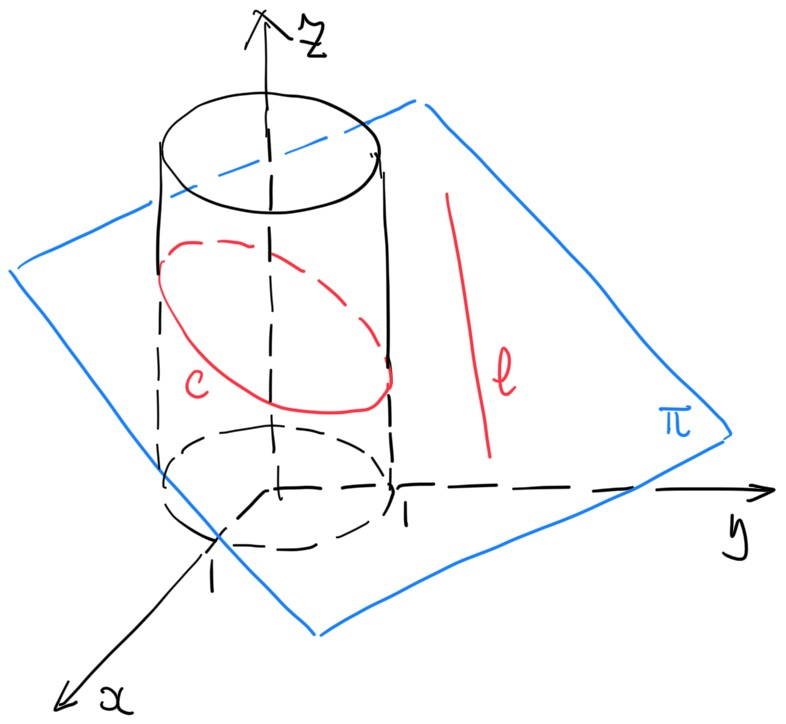
\includegraphics[width=0.5\textwidth]{./images/ch8/ccS.jpg}
	\end{center}
\end{frame}

\begin{frame}
	\linespread{1.5}
	
	\small \it
	设平面$\pi$与$xOy$平面的夹角为$\gamma$,注意到截面$S$在$xOy$平面上的投影为
	单位圆,故必有其面积$A=\df{\pi}{|\cos\gamma|}$,
	显然,当$|\cos\gamma|$取最大值时,截面$S$的面积最小。
	
	由已知,可设过$l$的平面束为
	$$\lambda(x-y)+\mu(x+z)=0,$$
	其方向向量为$\bm{n}=(\lambda+\mu,-\lambda,\mu)$,故
	$$\cos\gamma=\df{\bm{n}\cdot\bm{k}}{|\bm{n}||\bm{k}|}
	=\df{\mu}{\sqrt{2(\lambda^2+\lambda\mu+\mu^2)}}.$$
	不难解得,当$\frac{\lambda}{\mu}=-\df12$时,$|\cos\gamma|$取到最大值$\df{\sqrt6}3$。
	由此,令$\lambda=1,\mu=-2$,可得所求$\pi$的方程为
	$x+y+2z=0$。
\end{frame}

\begin{frame}
	\linespread{1.5}
	
	\small \it
	所求$\pi$的方程为
	$$x+y+2z=0.$$
	相应地曲线$C$可表示为
	$$\left\{\begin{array}{l}
		x^2+y^2=1\\
		x+y+2z=0
	\end{array}\right.$$
	不难求得其参数方程为
	$$\left\{\begin{array}{l}
		x=\cos t\\
		y=\sin t\\
		z=-\df12(\cos t+\sin t)
	\end{array}\right.
	\quad (t\in[0,2\pi])$$
	\fin
\end{frame}

\begin{frame}
	\linespread{1.5}
	\ba{3.画出以下空间区域的图形:	
	(1)曲面$(x-z)^2+y^2=1$与$z=-1,z=1$所围空间区域}
	
	\small 解:
	\begin{center}
		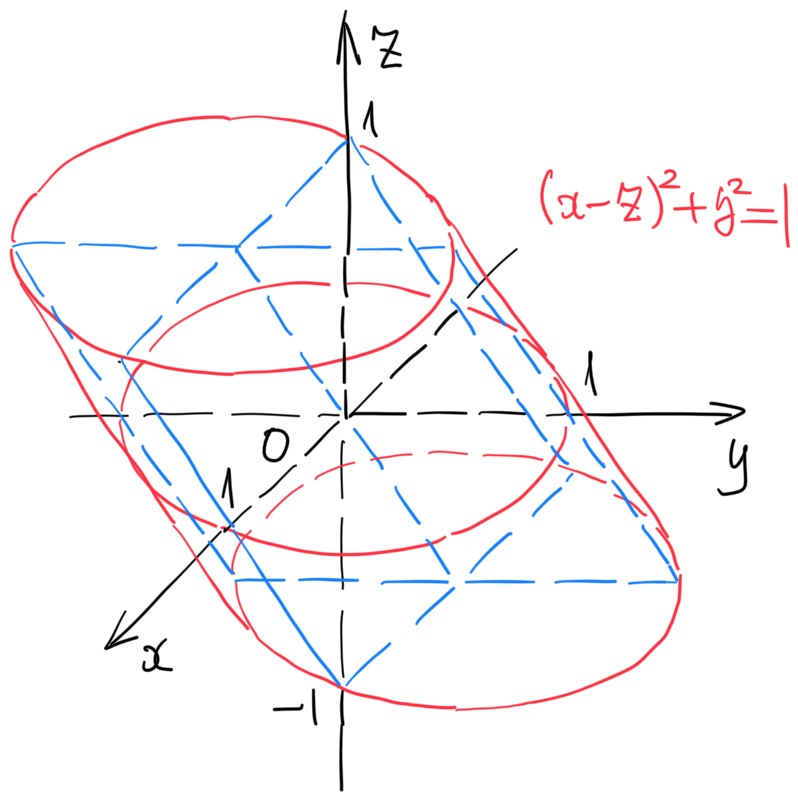
\includegraphics[width=0.5\textwidth]{./images/ch8/xzy-cl.jpg}
	\end{center}
\end{frame}


\begin{frame}
	\linespread{1.5}
	\ba{(2)$0\leq x\leq 1,0\leq y\leq x,0\leq z\leq xy$}
	
	\small 解:	
	\begin{center}
		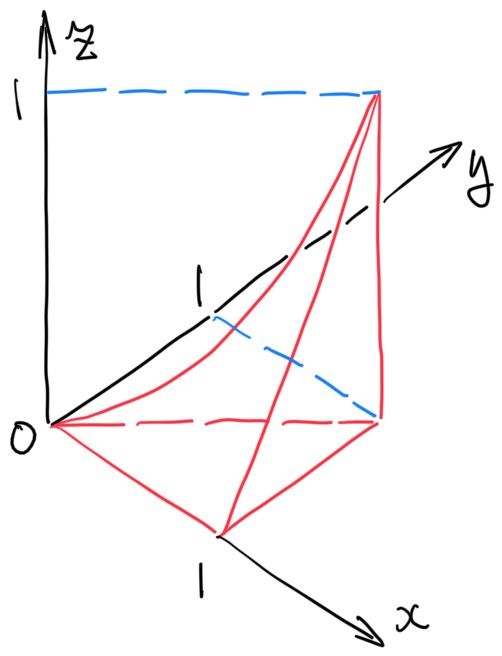
\includegraphics[width=0.4\textwidth]{./images/ch8/3int-1.jpg}\quad\quad
		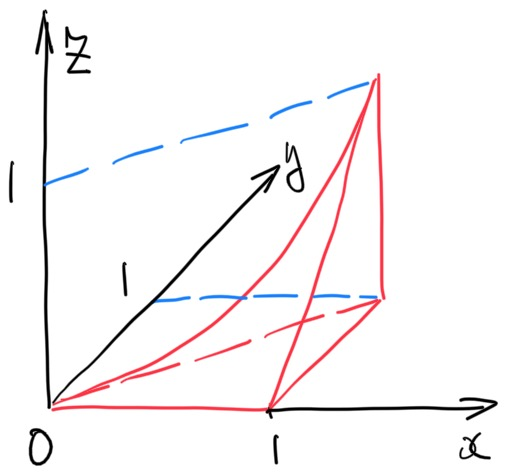
\includegraphics[width=0.45\textwidth]{./images/ch8/3int-2.jpg}
	\end{center}
	\fin
\end{frame}

\section{向量值函数}

\begin{frame}
	\linespread{1.5}
	\ba{1.证明向量值函数的求导法则:
	
	(1)$[\bm{u}(t)\cdot\bm{v}(t)]'
    =\bm{u}'(t)\cdot\bm{v}(t)+\bm{u}(t)\cdot\bm{v}'(t)$
    
    (2)$[\bm{u}(t)\times\bm{v}(t)]'
    =\bm{u}'(t)\times\bm{v}(t)+\bm{u}(t)\times\bm{v}'(t)$ 
    
    进而由此给出并证明三阶行列式
	  $$\left|\begin{array}{ccc}
	  	a_1(t) & a_2(t) & a_3(t)\\
	  	b_1(t) & b_2(t) & b_3(t)\\
	  	c_1(t) & c_2(t) & c_3(t)
	  \end{array}\right|$$
	  的求导法则。	 }
\end{frame}

\begin{frame}
	\linespread{1.5}
	
	\small 解:\it 令$\bm{a}=(a_1(t), a_2(t), a_3(t))$,
	$\bm{b}=(b_1(t), b_2(t), b_3(t))$,$\bm{c}=(c_1(t), c_2(t), c_3(t))$,
	应用以上的求导法则
	\begin{align*}
		&[(\bm{a}\times\bm{b})\cdot\bm{c}]'
		=(\bm{a}\times\bm{b})'\cdot\bm{c}+(\bm{a}\times\bm{b})\cdot\bm{c}'\\
		&=(\bm{a}'\times\bm{b})\cdot\bm{c}+(\bm{a}\times\bm{b}')\cdot\bm{c}
		+(\bm{a}\times\bm{b})\cdot\bm{c}'\\
		&=\left|\begin{array}{ccc}
  	a_1' & a_2' & a_3'\\
  	b_1 & b_2 & b_3\\
  	c_1 & c_2 & c_3
  \end{array}\right|
  +\left|\begin{array}{ccc}
  	a_1 & a_2 & a_3\\
  	b_1' & b_2' & b_3'\\
  	c_1 & c_2 & c_3
  \end{array}\right|
  +\left|\begin{array}{ccc}
  	a_1 & a_2 & a_3\\
  	b_1 & b_2 & b_3\\
  	c_1' & c_2' & c_3'
  \end{array}\right|.
	\end{align*}
	\fin
\end{frame}

\begin{frame}
	\linespread{1.5}
	\ba{2.Newton的万有引力定律可表述为
  $$\bm{F}=-\df{GmM}{r^3}\bm{r},$$
  其中$m$和$M$分别为行星和太阳的质量,$r$表示两者(球心)之间的距离,
  $\bm{r}$为由太阳中心指向行星中心的向量。
  \begin{enumerate}[(1)]
%     \setlength{\itemindent}{1cm}
    \item 求行星运动的加速度$\bm{r}''$;
    \item 证明行星总是运行在一个经过太阳中心的平面内,也即
    $\bm{r}\times\bm{r}'$为常向量。
  \end{enumerate}}
\end{frame}

\begin{frame}
	\linespread{1.5}
	\small 解:\it (1)由Newton第二定律,
	$$\bm{r}''=\df{\bm{F}}{m}=-\df{GM}{r^3}\bm{r}.$$
	
	(2)由向量值函数叉乘的求导法则,
	$$
		(\bm{r}\times\bm{r}')'
		=\bm{r}'\times\bm{r}'+\bm{r}\times\bm{r}''
		=\bm{r}\times\bm{r}''=-\bm{r}\times\df{GM}{r^3}\bm{r}=0,
	$$
	由此即知$\bm{r}\times\bm{r}'$为常向量。\fin
	
	\ba{注:本题等价于证明地球转动的角动量守恒,因此不能用角动量守恒来证明以上结论。}
\end{frame}

% \begin{frame}{出现的问题}
% 	\linespread{1.5}
% 	  \begin{itemize}%[<+-|alert@+>]
% 	    \item 作业进度慢!
% 	    \item 概念问题
% 	    \begin{itemize}
% 	      \item \b\it 幂级数展开不熟练
% 	      \item \b\it Maclaurin级数和关于$(x-x_0)$的幂级数分不清
% 	    \end{itemize}
% 	    \item 过程不规范或不完整
% 	    \begin{itemize}
% 	      \item \b\it 求收敛域要单独讨论端点的敛散性
% 	      \item \b\it 相同幂次的项要合并,并按幂次从小到大排列
% 	      \item \b\it 书写潦草随意\pause
% 	    \end{itemize}
% 	    \item \ba{雷同!!!}
% 	  \end{itemize}
% \end{frame}

% \begin{frame}
% 	\linespread{1.5}
% 	\ba{3.设$D$是由曲线$y=\sin x+1$与三条直线$x=0,x=\pi,y=0$
% 	所围成的曲边梯形,求$D$绕$x$轴旋转一周所围成的旋转体的体积。
% 	}
% 	\pause
% 	
% % 	\bigskip
% 	
% 	\begin{columns}
% 		\begin{column}{.5\textwidth}
% 			\begin{center}
% 				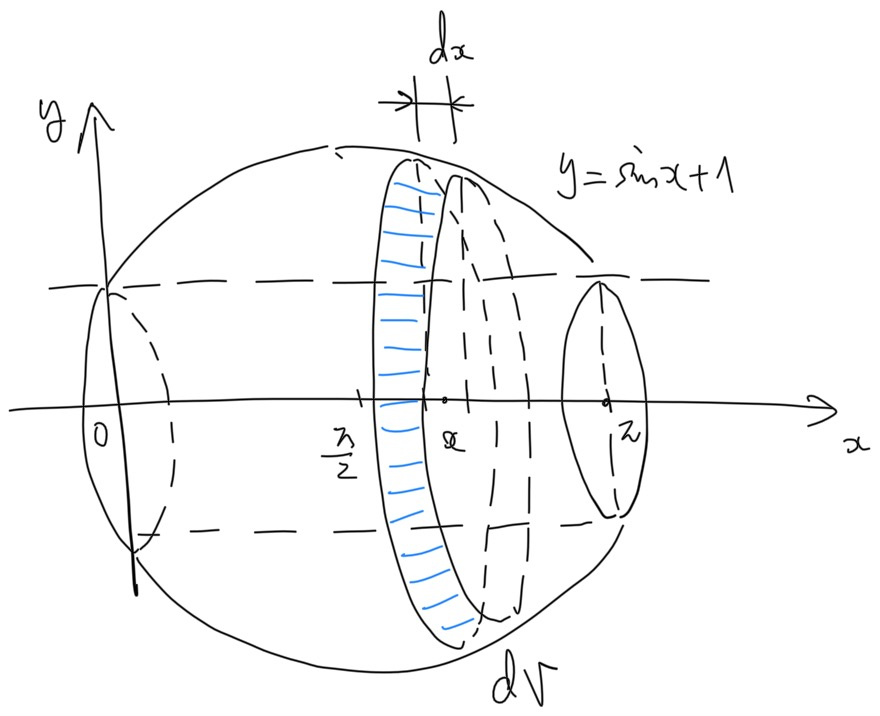
\includegraphics[width=.9\textwidth]{./images/ch6/sinx1cs.jpg}
% 		% 		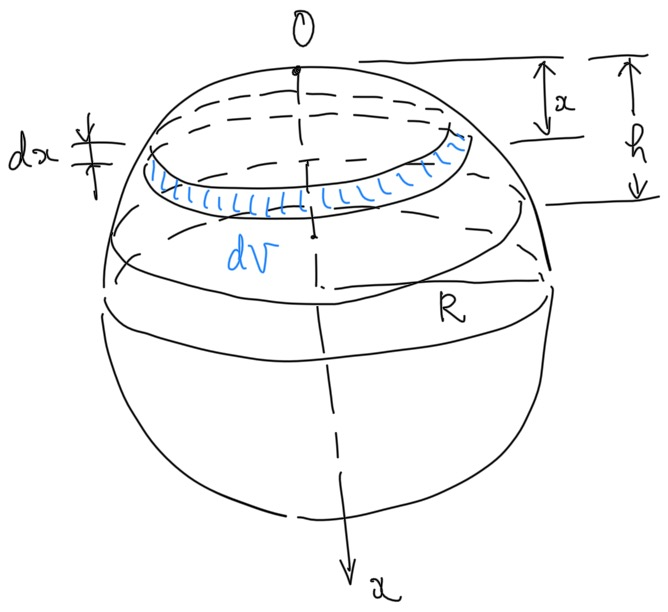
\includegraphics[width=6cm]{./images/ch6/topSp.jpg}
% 			\end{center}		
% 		\end{column}
% 		\begin{column}{.5\textwidth}
% 			\small 解:\it
% 			如图,体积微元$\d V=\pi y^2\d x$,	故所求体积
% 			$$
% 				V=\dint_0^{\pi}\pi(\sin x+1)^2\d x=\df32\pi^2.
% 			$$
% 		\end{column}
% 	\end{columns}
% \end{frame}

% !Mode:: "TeX:UTF-8"

\titlepage

\begin{frame}{说在前面}
	\linespread{1.5}
	  \begin{itemize}[<+-|alert@+>]
	    \item \ba{改错!改错!改错!}
% 	    \item 不记得自己哪周交作业
	  \end{itemize}
\end{frame}

% \begin{frame}{需要注意的问题}
% 	\linespread{1.5}
% 	  \begin{itemize}%[<+-|alert@+>]
% 	    \item L'Hospital法则
% 	    \begin{itemize}
% 	      \item \it 只能应用于“$\df{\bm{0}}{\bm{0}}$”
% 	      和“$\df{\bm{\infty}}{\bm{\infty}}$”型
% 	      \item \it 及时使用无穷小代换进行简化
% 	      \item \it 不正规的符号:\b 
% 	      $\xlongequal{\footnotesize\mbox{“L”}}$、
% 	      $\xlongrightarrow{\footnotesize\mbox{“L'Hospital法则”}}$、
% 	      $\df{\bm{0}}{\bm{0}}$、$\df{\bm{\infty}}{\bm{\infty}}$
% 	    \end{itemize}
% 	    \item Taylor公式
% 	    \begin{itemize}
% 	      \item \it Taylor多项式不包含余项
% 	      \item \it 合并同次幂的系数
% 	      \item \it 尽量按照幂次由低到高排列,最后写余项
% 	    \end{itemize}
% 	  \end{itemize}
% \end{frame}

\section{多元函数的极限与连续}

\begin{frame}
	\linespread{1.5}
	\ba{1.讨论以下二重极限的存在性:
	
	(1)$\lim\limits_{(x,y)\to(0,0)}\df{x+y}{\sqrt{x^2+y^2}}$}
	
	\bigskip
	
	\small 解:\it
	令$x=\rho\cos\theta,y=\rho\sin\theta$,其中$\theta$为常数,则
	$$\lim\limits_{(x,y)\to(0,0)}\df{x+y}{\sqrt{x^2+y^2}}
	=\lim\limits_{\rho\to 0}(\cos\theta+\sin\theta)=\cos\theta+\sin\theta,$$
	注意到右端结果与$\theta$相关,故该二重极限不存在。
	
	\ba{注:在以上解法中将$\theta$视为常数,相当于令$y=kx$,沿折线趋近原点}
\end{frame}

\begin{frame}
	\linespread{1.5}
	\ba{(2)$\lim\limits_{(x,y)\to(0,0)}\df{x+y}{\sqrt{x^2+y^2}}$}
	
	\bigskip
	
	\small 解:\it
	令$x=\rho\cos\theta,y=\rho\sin\theta$,则
	$$\lim\limits_{(x,y)\to(0,0)}\df{xy}{|x|+|y|}
	=\lim\limits_{\rho\to0}\df{\rho\cos\theta\sin\theta}{|\cos\theta|+|\sin\theta|},$$
	注意到$|\cos\theta|+|\sin\theta|\geq\sqrt2$,故对任意$\e>0$,令
	$\delta=\sqrt2\e$,则对任意$0<|\rho|<\delta$,总有
	$$\left|\df{\rho\cos\theta\sin\theta}{|\cos\theta|+|\sin\theta|}\right|
	\leq\df{\rho}{\sqrt2}<\e,$$
	由此可知,该二重极限存在。\fin
	
	\ba{注:证明极限存在时,不可简单地将$\theta$视为常数,否则与沿着$y=kx$趋近原点没有区别。
	仅仅证明沿着$y=kx$趋近时极限相同不能说明二重极限存在!}
\end{frame}

\begin{frame}
	\linespread{1.5}
	\ba{2.计算以下二重极限:}

	\bigskip
	
	\small 解:
	
	(1)$\lim\limits_{(x,y)\to(0,1)}\df{\ln(1+xy)}{y\sin x}
	=\lim\limits_{(x,y)\to(0,1)}\df{xy}{yx}=1.$
	
	(2)$\lim\limits_{(x,y)\to(0,0)}\df{1-\cos(xy)}{(x^2+y^2)e^{x^2}}
	=\lim\limits_{(x,y)\to(0,0)}\df{\frac12x^2y^2}{(x^2+y^2)}$
	
	$\quad\quad=\df12\lim\limits_{x\to
	0}\lim\limits_{y\to0}\df{x^2y^2}{x^2+y^2}=0.$
	
	(3)$\lim\limits_{(x,y)\to(0,0)}\df{e^{xy}-1}{\sqrt{2-e^{xy}}-1}
	=\lim\limits_{(x,y)\to(0,0)}\df{xy}{\frac12(1-e^{xy})}$
	
	$\quad\quad=-2\lim\limits_{(x,y)\to(0,0)}\df{xy}{xy}=-2.$
	\fin
	
	\ba{提示:合理使用无穷小代换可简化多重极限的运算。对于多重极限,不能
	随便使用L'Hospital法则!}
\end{frame}

\section{偏导数与全微分}

\begin{frame}
	\linespread{1.5}
	\ba{1.证明:$f(x,y)=\left\{\begin{array}{ll}
  	(x^2+y^2)\sin\df1{x^2+y^2}, & (x,y)\ne(0,0)\\
  	0, & (x,y)=(0,0)
  \end{array}\right.$
  的偏导函数在原点处不连续,但$f(x,y)$在原点处可微。}
	\pause

% 	\bigskip
	\small 证:\it
	$$f'_x(0,0)=\lim\limits_{\Delta x\to 0}
	\df{(\Delta x)^2\sin\frac1{(\Delta x)^2}-0}{\Delta x}=0,$$
	同理$f'_x(0,0)=0$。
	当$(x,y)\ne(0,0)$时,由偏导数的求导法则,
	$$f'_x(x,y)=2x\sin\df1{x^2+y^2}-\df{2x}{x^2+y^2}\cos\df1{x^2+y^2},$$
	$$f'_y(x,y)=2y\sin\df1{x^2+y^2}-\df{2y}{x^2+y^2}\cos\df1{x^2+y^2}.$$
\end{frame}

\begin{frame}
	\linespread{1.5}
	
	\small \it 偏导函数
	$$f'_x(x,y)=\left\{\begin{array}{ll}
  	2x\sin\df1{x^2+y^2}-\df{2x}{x^2+y^2}\cos\df1{x^2+y^2}, & (x,y)\ne(0,0)\\
  	0, & (x,y)=(0,0)
    \end{array}\right.$$
    注意到累次极限
	$$\lim\limits_{x\to 0}\lim\limits_{y\to 0}
	f'_x(x,y)
	=\lim\limits_{x\to 0}
	\left[2x\sin\df1{x^2}-\df{2}{x}\cos\df1{x^2}\right]
	=-\lim\limits_{x\to 0}
	\df{2}{x}\cos\df1{x^2}$$
	不存在,故二重极限$\lim\limits_{(x,y)\to(0,0)}f'_x(x,y)$
	不存在,从而可知偏导函数$f'_x(x,y)$在原点处不连续。
	
	同理可证$f'_y(x,y)$在原点处不连续。
\end{frame}

\begin{frame}
	\linespread{1.5}
	
	\small \it 进一步,注意到极限
	\begin{align*}
		&\lim\limits_{(x,y)\to(0,0)}\df{f(\Delta x,\Delta y)-f'_x(0,0)\Delta x
		-f'_y(0,0)\Delta y}{\sqrt{(\Delta x)^2+(\Delta y)^2}}\\
		&=\lim\limits_{(x,y)\to(0,0)}\sqrt{(\Delta x)^2+(\Delta y)^2}
		\sin\df1{(\Delta x)^2+(\Delta y)^2}=0,
	\end{align*}
	故
	$$f(\Delta x,\Delta y)-f'_x(0,0)\Delta x-f'_y(0,0)\Delta y
	=\circ(\sqrt{(\Delta x)^2+(\Delta y)^2}),$$
	也即$f(x,y)$在原点处可微。\fin
	
	\ba{要点:讨论二重极限的存在性!可微的证明方法!}
\end{frame}

\begin{frame}
	\linespread{1.5}
	\ba{2.求$z=\arctan\df{x+y}{1-xy}$的所有二阶偏导数。}
	\pause

% 	\bigskip
	\small 解:\it
	注意到
	$$\arctan\df{x+y}{1-xy}=\arctan x+\arctan y,$$
	故
	\begin{align*}
		&z'_x=\df1{1+x^2},\quad\quad\quad
		z'_y=\df1{1+y^2},\\
		&z''_{xx}=-\df{2x}{(1+x^2)^2},\quad
		z''_{yy}=-\df{2y}{(1+y^2)^2},\\
		&z''_{xy}=z''_{yx}=0.
	\end{align*}
	\fin
\end{frame}

\begin{frame}
	\linespread{1.5}
	\ba{3.已知$\df{\p z}{\p y}=\df{x^2+y^2}y$,$z(x,1)=e^x$,
	求$z(x,y)\;(y\ne0)$。}
	\pause

% 	\bigskip
	\small 解:\it
	由$\df{\p z}{\p y}=\df{x^2+y^2}y=\df{x^2}y+y$,可知
	$$z(x,y)=x^2\ln|y|+\df12y^2+u(x),$$
	其中$u(x)$是某个关于$x$的一元函数。又$z(x,1)=e^x$,也即
	$$e^x=\df12+u(x)\quad
	\Rightarrow\quad u(x)=e^x-\df12,$$
	故
	$$z(x,y)=x^2\ln|y|+\df12(y^2-1)+e^x.$$
	\fin
\end{frame}

\begin{frame}
	\linespread{1.5}
	\ba{4.设$z=\dint_x^{xy}e^{(t-x)^2}\d t$,
	求$\df{\p z}{\p x}$和$\df{\p z}{\p y}$。}
	\pause

% 	\bigskip
	\small 解:\it
	令$u=t-x$,则
	$$z=\dint_0^{x(y-1)}e^{u^2}\d u.$$
	进而
	$$
		z'_x=(y-1)e^{x^2(y-1)^2},\quad z'_y=xe^{x^2(y-1)^2}.
	$$
	\fin
	
	\ba{提醒:不要忘记变限积分求导的基本方法!}
\end{frame}

\begin{frame}
	\linespread{1.5}
	\ba{5.求函数$z=xy^2$在$(1,2)$附近且$(\Delta x,\Delta y)=(0.1,-0.5)$时
	对应的函数值的改变量(全增量)与全微分。}
	
% 	\bigskip
	
	\small 解:\it 
	全增量
	$$\Delta z=z(1.1,1.5)-z(1,2)=-1.525,$$
	注意到$z'_x(1,2)=z'_y(1,2)=4$,故全微分
	$$\d z=z'_x(1,2)\Delta x+z'_y(1,2)\Delta y
	=4\cdot 0.1+4\cdot(-0.5)=-1.6.$$
	\fin
	
	\ba{注意:$x,y$为自变量,故$\d x=\Delta x,\d y=\Delta y$,
	给定了$\Delta x,\Delta y$的值,微分的值是可以具体计算出来的!}
\end{frame}

\begin{frame}
	\linespread{1.5}
	\ba{6.利用微分计算$\sqrt{1.02+(1.97)^3}$的近似值。}
	
	\small 解:\it
	考虑函数$z=\sqrt{x+y^3}$,则
	$$z(1,2)=3,\quad z'_x(1,2)=\df16,\quad z'_y(1,2)=2.$$
	进而可知
	$$\sqrt{1.02+(1.97)^3}
	\approx z(1,2)+z'_x(1,2)\cdot0.02+z'_y(1,2)\cdot(-0.03)
	\approx 2.943.$$
	\fin
\end{frame}

\section{补充例题}

\begin{frame}
	\linespread{1.5}
	\ba{例:设$u=u(x)$由
	$$u=f(x,y),\;g(x,y,z)=0,\;h(x,z)=0$$
	确定,$f,g,h$一阶偏导连续,$h'_z\ne0,g'_y\ne0$,求$\df{\p u}{\p x}$}
\end{frame}

\begin{frame}
	\linespread{1.5}
	\ba{例:设$f(u)$当$u>0$时二阶可导,且$z=f(\sqrt{x^2+y^2})$满足方程
	$$\df{\p^2z}{\p x^2}+\df{\p^2z}{\p y^2}=0,$$
	\begin{enumerate}[(1)]
% 	  \setlength{\itemindent}{1cm}
	  \item 证明:$uf''(u)+f'(u)=0$;
	  \item 设$f(1)=0,f'(1)=1$,求$f(u)$。 
	\end{enumerate}}
\end{frame}

\begin{frame}
	\linespread{2}
	\ba{例:设$u(x,y)$满足
	$$\df{\p^2 u}{\p x^2}-\df{\p^2 u}{\p y^2}
	+k\left(\df{\p u}{\p x}+\df{\p u}{\p y}\right)=0.$$
	试选择合适的$a,b$,使得通过变换$u(x,y)=v(x,y)e^{ax+b}$后,所得
	新的方程不再含有任何偏导数项。}
\end{frame}

% \begin{frame}{出现的问题}
% 	\linespread{1.5}
% 	  \begin{itemize}%[<+-|alert@+>]
% 	    \item 作业进度慢!
% 	    \item 概念问题
% 	    \begin{itemize}
% 	      \item \b\it 幂级数展开不熟练
% 	      \item \b\it Maclaurin级数和关于$(x-x_0)$的幂级数分不清
% 	    \end{itemize}
% 	    \item 过程不规范或不完整
% 	    \begin{itemize}
% 	      \item \b\it 求收敛域要单独讨论端点的敛散性
% 	      \item \b\it 相同幂次的项要合并,并按幂次从小到大排列
% 	      \item \b\it 书写潦草随意\pause
% 	    \end{itemize}
% 	    \item \ba{雷同!!!}
% 	  \end{itemize}
% \end{frame}

% \begin{frame}
% 	\linespread{1.5}
% 	\ba{3.设$D$是由曲线$y=\sin x+1$与三条直线$x=0,x=\pi,y=0$
% 	所围成的曲边梯形,求$D$绕$x$轴旋转一周所围成的旋转体的体积。
% 	}
% 	\pause
% 	
% % 	\bigskip
% 	
% 	\begin{columns}
% 		\begin{column}{.5\textwidth}
% 			\begin{center}
% 				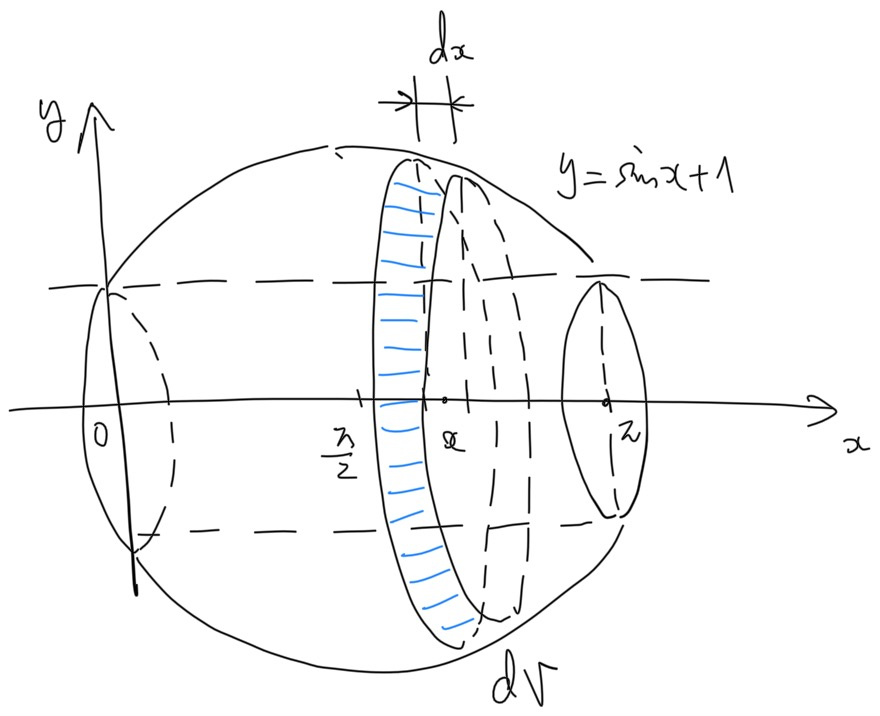
\includegraphics[width=.9\textwidth]{./images/ch6/sinx1cs.jpg}
% 		% 		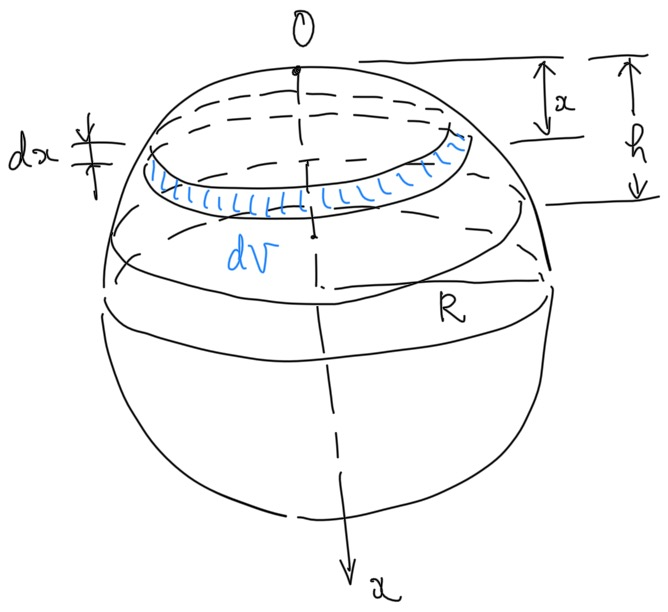
\includegraphics[width=6cm]{./images/ch6/topSp.jpg}
% 			\end{center}		
% 		\end{column}
% 		\begin{column}{.5\textwidth}
% 			\small 解:\it
% 			如图,体积微元$\d V=\pi y^2\d x$,	故所求体积
% 			$$
% 				V=\dint_0^{\pi}\pi(\sin x+1)^2\d x=\df32\pi^2.
% 			$$
% 		\end{column}
% 	\end{columns}
% \end{frame}

% % !Mode:: "TeX:UTF-8"

\titlepage

\begin{frame}{随堂测验}
	\linespread{1.5}
	  \begin{itemize}
	    \item \ba{5道极限计算题,20分钟}
	    \item \ba{5道积分计算题,20分钟}
	    \item \ba{每题10分}
	    \item \ba{不必抄题}
	    \item \ba{成绩记入期末总评}
	  \end{itemize}
\end{frame}

\begin{frame}{计算下列极限}
	\linespread{1.5}
	\large
	\begin{columns}
		\begin{column}{0.5\textwidth}
			1.\;$\limx{0^+}\df{1-\cos x\cos\sqrt x}x$\\[1ex]
			2.\;$\limx{\infty}\left(\df{x+3}{x+1}\right)^{\sin\frac1x}$\\[1ex]
			3.\;$\limn\sqrt{\df{n-k}{n^3}}$
		\end{column}
		\begin{column}{0.5\textwidth}
			\\[4ex]
			4.\;$\limx0\df{x-\sin x}{x^2\arctan x}$\\[1ex]
			5.\;$\limx0\df{e^{-\frac{x^2}2}-\cos x}{\sqrt[4]{1+x^4}-1}$
		\end{column}
	\end{columns}
\end{frame}

\begin{frame}{计算下列积分}
	\linespread{1.5}
	\large
	\begin{columns}
		\begin{column}{0.5\textwidth}
			6.\;$\dint\df{\d x}{\cos x}$\\[1ex]
			7.\;$\dint\df{\d x}{x^2-x+1}$\\[1ex]
			8.\;$\dint_0^3\df{\sqrt x\d x}{\sqrt x+\sqrt{3-x}}$
		\end{column}
		\begin{column}{0.5\textwidth}
% 			\\[4ex]
			9.\;$\dint\tan^3x\sec^3x\d x$\\[1ex]
			10.\;$\dint_{-1}^0\df{\ln(1+x)\d x}{\sqrt{1+x}}$
		\end{column}
	\end{columns}
\end{frame}

\begin{frame}
	\Huge
	\ba{TIME'S UP!!!}
\end{frame}

%   % !Mode:: "TeX:UTF-8"

\begin{frame}
	\frametitle{常微分方程习题课}
	\linespread{1.5}
	  \begin{itemize}
% 	    \item 理解微分方程及其相关概念
	    \item 一阶微分方程解法与常用解题技巧
	    \item 两类可降阶的二阶方程的解法及其高阶推广
	    \item 二阶线性微分方程解的结构
	    \item 解二阶常系数齐次线性微分方程的特征方程法及其高阶推广
	    \item 解两类二阶常系数非齐次线性微分方程的待定系数法
	  \end{itemize}
\end{frame}

\section{问题讨论}

\begin{frame}{问题讨论}
	\linespread{1.5}
	\alert{问:}已知$n$阶线性微分方程的$n$个解,
	能否写出这个微分方程及其通解?\pause\\[1ex]
	
	\alert{答:}{\it 不一定!}\pause {\it 除非 
	这$n$个解恰好线性无关。} \pause 
	
	\bigskip
	\alert{问:}适当确定微分方程通解中的参数值,可以得到其任意的特解?\pause \\[1ex]
	
	\alert{答:}{\it 错!}\pause 反例:{\it $y'=\sin x\cos^2y$}.
\end{frame}

\begin{frame}{问题讨论}
	\linespread{1.2}
	\alert{问:}$y_1=(x-1)^2$和$y_2=(x+1)^2$都是方程
	$$(x-1)^2y''-2xy'+2y=0,$$
	和
	$$2yy''-(y')^2=0$$
	的解。但二者的线性组合
	$$y=C_1(x-1)^2+C_2(x+1)^2,\;(C_1,C_2\in\mathbb{R})$$
	却仅能满足前一个方程,为什么?\pause 
	
	\alert{答:}{\it 第二个方程不是线性方程!}
\end{frame}

\section{补充例题}

\begin{frame}{填空}
	\linespread{2}
	\ba{1.}\;$y''+4y'+4y=1$的通解为
	\underline{\uncover<2->{\;\b{$(C_1+C_2x)e^{-2x}+1/4$}}\;}.\\[1em]
	
	\ba{2.}\;设$e^x(C_1\cos x+C_2\sin x)$为首项系数为$1$的某二阶常系数
	齐次线性微分方程的通解,则该微分方程为
	\underline{\uncover<3->{\;\b{$y''-2y'+2y=0$}}\;}.\\[1em]
	
	\ba{3.}\;设$\cos x$与$xe^x$分别为某$n$阶常系数齐次线性微分方程的两个解,
	则最小的$n=$\underline{\uncover<4->{\;\b{$4$}}\;},相应的首项
	系数为$1$的方程为\underline{\uncover<5->{\;\b{$
	y^{(4)}-2y^{(3)}+2y''-2y'+y=0$}\;}}
	
% 	方程$xy''-2xy'+2y=x\ln x$的通解为
% 	为\underline{\uncover<6->{\;\b{$
% 	C_1x+C_2x^2-\left(\df12\ln^2x+\ln x\right)x$}\;}}
\end{frame}

\begin{frame}{选择}
	\linespread{1.5}
	\ba{1.}\;方程$y''+4y=e^{3x}+x\sin 2x$的一个特解形式是
	(\underline{\uncover<2->{\;\b{A}}\;})
	\begin{enumerate}[(A)]
	  \item $Ae^{3x}+x[(Bx+C)\cos2x+(Dx+E)\sin2x]$
	  \item $Ae^{3x}+(Bx+C)\cos2x+(Dx+E)\sin2x$
	  \item $Axe^{3x}+x[(Bx+C)\cos2x+(Dx+E)\sin2x]$
	  \item $Axe^{3x}+(Bx+C)\cos2x+(Dx+E)\sin2x$
	\end{enumerate}
\end{frame}

\begin{frame}{选择}
	\linespread{1.3}
	\ba{2.}\;设$y_1(x),y_2(x),y_3(x)$为方程
	$$y''+p(x)y'+q(x)y=f(x)$$
	的三个线性无关的解,$C_1,C_2$为任意常数,则该非齐次线性微分方程的通解为
	(\underline{\uncover<2->{\;\b{C}}\;})
	\begin{enumerate}[(A)]
	  \item $(C_1+C_2)y_1+(C_2-C_1)y_2+(1-C_2)y_3$
	  \item $(C_1+C_2)y_1+(C_2-C_1)y_2+(C_1-C_2)y_3$
	  \item $C_1y_1+(C_2-C_1)y_2+(1-C_2)y_3$
	  \item $C_1y_1+(C_2-C_1)y_2+(C_1-C_2)y_3$
	\end{enumerate}
\end{frame}

\begin{frame}{选择}
	\linespread{1.3}
	\ba{3.}\;设$y=f(x)$为方程$y''-2y'+4y=0$
	的一个解,若$f(x_0)>0,f'(x_0)=0$,
	则函数$f(x)$在$x_0$
	(\underline{\uncover<2->{\;\b{A}}\;})
	\begin{enumerate}[(A)]
	  \item 取极大值
	  \item 取极小值
	  \item 的某个领域内单调增加
	  \item 的某个领域内单调减少
	\end{enumerate}
\end{frame}

\begin{frame}{选择}
	\linespread{1.3}
	\ba{4.}\;设$y(x)$为方程$y''+py'+qy=e^{3x}$满足初始条件$y(0)=y'(0)=0$
	的解,则$\limx{0}\df{\ln(1+x^2)}{y(x)}$
	(\underline{\uncover<2->{\;\b{C}}\;})
	\begin{enumerate}[(A)]
	  \item 不存在
	  \item 等于$1$
	  \item 等于$2$
	  \item 等于$3$
	\end{enumerate}
\end{frame}

\begin{frame}{选择}
	\linespread{1.3}
	\ba{5.}\;设$y(x)$满足$x\d y+(x-2y)\d x=0$,且曲线$y=y(x)$与直线$x=1$
	及$x$轴所围平面图形绕$x$轴旋转所得旋转体的体积最小,则$y(x)=$
	(\underline{\uncover<2->{\;\b{C}}\;})
	\begin{enumerate}[(A)]
	  \item $x-\df14x^2$
	  \item $x+\df54x^2$
	  \item $x-\df54x^2$
	  \item $x+\df14x^2$
	\end{enumerate}
\end{frame}

\begin{frame}{选择}
	\linespread{1.3}
	\ba{6.}\;方程$y''+by'+y=0$的每个解都在$x>0$上有界,则实数$b$的取值范围是
	(\underline{\uncover<2->{\;\b{A}}\;})
	\begin{enumerate}[(A)]
	  \item $[0,+\infty)$
	  \item $(-\infty,0]$
	  \item $(-\infty,4]$
	  \item $(-\infty,+\infty]$
	\end{enumerate}
\end{frame}

% \begin{frame}{解方程}
% 	\linespread{1.5}
% 	\begin{enumerate}
% 	  \item $xy'\ln x+y=\ln x$.\hfill \b$t=\ln x$
% 	\end{enumerate}
% \end{frame}

\begin{frame}{解答题}
	\linespread{1.2}
	\ba{1.}\;设$f(x)$为连续函数,且
	$$f(x)=e^{-x}+\dint_0^xf(t)\d t,$$
	求$f(x)$.
	
	\pause\alert{提示:}\it\b  积分方程通常自带初值条件$f(0)=1$.\pause
	$$f'(x)-f(x)=-e^{-x}\quad\Rightarrow\quad 
	f(x)=\df12(e^x+e^{-x}).$$
	
	\pause 不带初值条件的例子:\ba{习题7.2-8}
\end{frame}

\begin{frame}{解答题}
	\linespread{1.2}
	\ba{2.}\;设$f(x)$为连续函数,且
	$$f(x)=e^{2x}+\dint_0^xtf(x-t)\d t,$$
	求$f(x)$.
	
	\pause\alert{提示:}\it\b $f(0)=1,f'(0)=2$\pause  
	$$f''(x)-f(x)=4e^{2x}\quad\Rightarrow\quad 
	f(x)=-\df12e^x+\df16e^{-x}+\df43e^{2x}.$$
\end{frame}

% \begin{frame}{解答题}
% 	\linespread{1.2}
% 	\ba{3.(习题7.3-7)}函数$y(x)\;(x\geq 0)$二阶可导,$y'(x)>0$,
% 	$y(0)=1$,过其上任一点$(x,y)$作曲线的切线和至$x$轴的垂线,该两直线
% 	与$x$轴所围成的三角形面积记为$S_1(x)$,又区间$[0,\alert{x}]$
% 	(\alert{\it 此处教材印刷错误!})上以$y(x)$为曲边
% 	的曲边梯形面积记为$S_2(x)$。已知$2S_1-S_2=1$,求$y(x)$。
% 	
% 	\pause\alert{提示:}\it\b   
% 	$$\df{y^2}{y'}-\dint_0^xy(t)\d t=1\quad\Rightarrow\quad 
% 	yy''=(y')^2,\;y'(0)=1.$$
% 	\pause 结合$y(0)=1$,解得$y=e^x$.
% \end{frame}

\begin{frame}{解答题}
	\linespread{1.2}
	\ba{3.}\;设对任意$x,y\in\mathbb{R}$
	$$f(x+y)=f(x)e^y+f(y)e^x,$$
	$f'(0)=a\ne 0$,求$f(x)$.
	
	\pause\alert{提示:}\it\b 必须用定义计算$f'(x)$,
	$$\lim\limits_{\Delta x\to 0}\df{f(x+\Delta x)-f(x)}{\Delta x}
	=f(x)+ae^x.$$
	\pause 类似题目:\alert{\bf 习题7.2-7,辅导书(下)-P256-例5}
\end{frame}

\begin{frame}{解答题}
	\linespread{1.2}
	\ba{4.}\;某同学将乘积的导数公式错误地记作$(fg)'=f'g'$,然而在一次求导时
	居然得到了正确的结果。目前知道他使用的$f(x)=e^{x^2},(x>1/2)$,
	问他用到的$g(x)$可能是什么?
	
	\pause\alert{提示:}\it\b  
	$$\left(e^{x^2}g\right)'=\left(e^{x^2}\right)'g'$$
	从而$(2x-1)g'=2xg$,解得
	$$g=Ce^x\sqrt{2x-1}$$
\end{frame}

\begin{frame}{解答题}
	\linespread{1.5}
	\ba{5.}\;设二阶常系数线性微分方程
	$$y''+\alpha y'+\beta y=\gamma e^x$$
	的一个解为$y=e^{2x}+(1+x)e^x$,试确定其中的常数$\alpha,\beta,\gamma$.
	
	\pause\alert{提示:}\it\b $\alpha=-3,\beta=2,\gamma=-1$.
\end{frame}

\begin{frame}{解答题}
	\linespread{1.2}
	\ba{6.}\;求方程$y''+2y'+2y=2e^{-x}\cos^2\df x2$的通解.
	
	\pause\alert{提示:}\it\b 
	$$2e^{-x}\cos^2\df x2=e^{-x}+e^{-x}\cos x,$$
	利用叠加原理分别求解两个常系数非齐次线性微分方程。
\end{frame}

% \begin{frame}{解答题}
% 	\linespread{1.2}
% 	\alert{(2003考研)} 设$y(x)$在$\mathbb{R}$上具有二阶连续导数,
% 	$y'\ne 0$,$x=x(y)$为其反函数。
% 	\begin{enumerate}
% 	  \item 试将$x=x(y)$所满足的微分方程
% 	  $$\df{\d^2x}{\d y^2}+(y+\sin x)\left(\df{\d x}{\d y}\right)^3=0$$
% 	  变换为$y=y(x)$所满足的微分方程;
% 	  \item 求变换后的微分方程满足初始条件$y(0)=0$和$y'(0)=1.5$的解。
% 	\end{enumerate}
% 	
% 	\pause\alert{提示:}\it\b 
% 	$y''-y=\sin x\quad\Rightarrow\quad y=e^x-e^{-x}-\df12\sin x $
% \end{frame}

\begin{frame}{应用题}
	\linespread{1.2}
	\ba{7.}\;令$t=\tan x$,将方程
	$$\cos^4xy''_{xx}+2\cos^2x(1-\sin x\cos x)y'_x+y=e^{-\tan x}$$
	变换为$y$关于$t$的微分方程,并求其通解。
	
	\pause\alert{提示:}\it\b 
	$$y''_{tt}+2y'_t+y=e^{-t}$$
	$$y=\left(C_1+C_2\tan x+\df12\tan^2x\right)e^{-\tan x}$$
\end{frame}

\section{微分方程的应用}

\begin{frame}{应用题}
	\linespread{1.4}
	\ba{8.}\;已知某凹曲线任一点处的曲率为$\df1{2y^2\cos\alpha}$,其中
	$\alpha$为该点处的切线倾角($\cos\alpha>0$),且曲线在
	点$(1,1)$处的切线是水平的,求该曲线的方程。
	
	\pause\alert{提示:}\it\b $\cos\alpha>0=\df1{\sqrt{1+(y')^2}},
	\;y''>0$
	$$2y^2y''=[1+(y')^2]^2\quad\Rightarrow\quad
	4y=(x-1)^2+4$$
\end{frame}

% \begin{frame}{应用题}
% 	\linespread{1.2}
% 	\ba{(习题7.4-14)}一根挂在钉子上的链条,最初两端距离钉子
% 	分别为$8$m和$12$m,如不计钉子
% 	对链条产生的摩擦力,求链条从钉子上完全滑落所需的时间。
% 	
% 	\pause\alert{提示:}\it\b 设$x$为较长一端端点据钉子的距离
% 	$$\left\{\begin{array}{l}
% 		x''-\df g{10}x=-g\\
% 		x(0)=12\\
% 		x'(0)=0
% 	\end{array}\right.$$
% % 	\pause
% % 	\alert{思考:}若摩擦力等于$1$m长的链条的重量,模型又是怎样的?
% \end{frame}

\begin{frame}{应用题}
	\linespread{1.2}
	\ba{9.}\;已知某车间容积$V$,其空气中CO$_2$的密度为$\rho_1$,现以CO$_2$浓度$\rho_2(<<\rho_1)$的
	新鲜空气输入,问每分钟应输入多少才能在$T$分钟后使车间中CO$_2$的含量不超过$\rho_0$。
	(注:假设新注入的空气能够与原有空气立即混合达到均匀,且空气不会被压缩。)

	\pause\alert{提示:}\it\b 设$t$分钟时的$CO_2$含量为$C(t)$,
	$$C'=\rho_2V_1-C\df{V_1}{V},C(0)=\rho_1V$$
\end{frame}

\begin{frame}{应用题}
	\linespread{1.2}
	\ba{10.}\;某湖泊的水量为$V$,每年排入湖内的污水和净水量均为$V/6$,且湖内的总水量不变。
	已知1999年底湖内的污染物含量为$5m_0$。为了治理污染,从2000初开始,限定排入
	湖中的污水中污染物浓度不得超过$m_0/V$。问至少需要经过多少年,
	湖内的污染物含量能够降至$m_0$以下?(注:假设湖水中的污染物浓度时均匀分布的。)

	\pause\alert{提示:}\it\b 
	$$m'=\df{m_0}6-\df m3,\quad m=\df{m_0}2(1+9e^{-t/3})$$
	$t=6\ln3$年后,达到要求。
\end{frame} %常微分方程习题课
% 	\begin{frame}{向量的运算、空间平面与直线}
	\linespread{1.2}
	\begin{enumerate}
	  \item 内积(投影)、外积(面积)、混合积(体积,三线共面)
	  \item 平面方程中的几何特征
	  \item 不同直线方程间的相互转换
	  \item 空间几何问题的一题多解
	\end{enumerate}
\end{frame}

\begin{frame}{判断}
	\linespread{1.2}
	\begin{enumerate}
	  \item $\bm{a}\cdot\bm{a}\cdot\bm{a}=\bm{a}^3$\quad\pause\ba{$\times$}\pause
	  \item $\bm{a}\ne 0$时,$\df{\bm{a}}{\bm{a}}=1$\quad\pause\ba{$\times$}\pause
	  \item $\bm{a}(\bm{a}\cdot\bm{b})=\bm{a}^2\bm{b}$
	    \quad\pause\ba{$\times$}\pause
	  \item $(\bm{a}\cdot\bm{b})^2=\bm{a}^2\bm{b}^2$\quad\pause\ba{$\times$}\pause
	  \item $|\bm{a}\cdot\bm{b}|=|\bm{a}|\cdot|\bm{b}|$
		\quad\pause\ba{$\times$}\pause
	  \item $(\bm{a}+\bm{b})\times(\bm{a}-\bm{b})=\bm{a}\times\bm{a}
  		-\bm{b}\times\bm{b}=0$
  		\quad\pause\ba{$\times$}\pause
  	  \item $\bm{a}\ne 0$时,$\bm{a}\cdot\bm{b}
  	  	=\bm{a}\cdot\bm{c}\Rightarrow\bm{b}=\bm{c}$
  	  	\quad\pause\ba{$\times$}\pause
  	  \item  $\bm{a}\ne 0$时,$\bm{a}\times\bm{b}
  	  	=\bm{a}\times\bm{c}\Rightarrow\bm{b}=\bm{c}$
  	  	\quad\pause\ba{$\times$}
	\end{enumerate}
\end{frame}

\begin{frame}{填空}
	\linespread{1.2}
	\ba{1.}\;设$(\bm{a}\times\bm{b})\bm{c}=2$,则
	$[(\bm{a}+\bm{b})\times(\bm{b}+\bm{c})](\bm{c}+\bm{a})=$
	\underline{\uncover<2->{\;\b{$4$}}\;}.\\[1em]
	
	\ba{2.}\;设$\bm{a},\bm{b}$均为非零向量,则
	其角平分线上的向量为
	\underline{\uncover<3->{\;\b{$C\left(\df{\bm{a}}{|\bm{a}|}
	+\df{\bm{b}}{|\bm{b}|}\right),\;(C\in\mathbb{R})$}}\;}.\\[1em]
	
	\ba{3.}\;设$\bm{a},\bm{b},\bm{c}$均为非零向量,且$\bm{a}=\bm{b}\times\bm{c}$,
	$\bm{b}=\bm{c}\times\bm{a}$,
	$\bm{c}=\bm{a}\times\bm{b}$则
	$|\bm{a}|+|\bm{b}|+|\bm{c}|=$
	\underline{\uncover<4->{\;\b{$3$}}\;}.\\[1em]
\end{frame}

\begin{frame}{填空}
	\linespread{1.2}
	\ba{4.}\;设$|\bm{a}|=2,|\bm{b}|=2$,$\bm{a}$和$\bm{b}$
	的夹角为$\pi/3$,则$|2\bm{a}-3\bm{b}|=$
	\underline{\uncover<2->{\;\b{$2\sqrt7$}}\;}.\\[1em]
	
	\ba{5.}\;设$\bm{a},\bm{b}$均为非零向量,且$|\bm{b}|=1$,$\bm{a}$和$\bm{b}$
	的夹角为$\pi/4$,则$\limx{0}\df{|\bm{a}+x\bm{b}|-|\bm{a}|}{x}=$
	\underline{\uncover<3->{\;\b{$\df{\sqrt2}2$}}\;}.\\[1em]
	
	\ba{6.}\;平面$Ax+By+Cz+D_i=0\;(i=1,2)$之间的距离为
	\underline{\uncover<4->{\;\b{$\df{|D_1-D_2|}{\sqrt{A^2+B^2+C^2}}$}}\;}.
\end{frame}

\begin{frame}{选择}
	\linespread{1.3}
	\ba{1.}\;设$\bm{a},\bm{b},\bm{c}$均为非零向量,则与$\bm{a}$不垂直的是
	(\underline{\uncover<2->{\;\b{D}}\;})
	\begin{enumerate}[(A)]
	  \item $(\bm{a}\cdot\bm{c})\bm{b}-(\bm{a}\cdot\bm{b})\bm{c}$
	  \item $\bm{b}-\left(\df{\bm{a}\cdot\bm{b}}{\bm{|a|}^2}\right)\bm{a}$
	  \item $\bm{a}\times\bm{b}$
	  \item $\bm{a}+(\bm{a}\times\bm{b})\times\bm{a}$
	\end{enumerate}
\end{frame}

\begin{frame}{选择}
	\linespread{1.3}
	\ba{2.}\;设$\bm{a},\bm{b}$为非零向量,$|\bm{a}-\bm{b}|=|\bm{a}+\bm{b}|$,则
	(\underline{\uncover<2->{\;\b{C}}\;})
	\begin{enumerate}[(A)]
	  \item $\bm{a}-\bm{b}=\bm{a}+\bm{b}$
	  \item $\bm{a}=\bm{b}$
	  \item $\bm{a}\cdot\bm{b}=0$
	  \item $\bm{a}\times\bm{b}=0$
	\end{enumerate}
\end{frame}

\begin{frame}{选择}
	\linespread{1.3}
	\ba{3.}\;设$\bm{a},\bm{b}$为非零向量,且满足
	$(\bm{a}+3\bm{b})\perp(7\bm{a}-5\bm{b})$,
	$(\bm{a}-4\bm{b})\perp(7\bm{a}+2\bm{b})$,则
	向量$\bm{a}$和$\bm{b}$的夹角为
	(\underline{\uncover<2->{\;\b{C}}\;})
	\begin{enumerate}[(A)]
	  \item $0$
	  \item $\pi/2$
	  \item $\pi/3$
	  \item $2\pi/3$
	\end{enumerate}
\end{frame}

\begin{frame}{选择}
	\linespread{1.3}
	\ba{4.}\;设平面$\pi$位于平面$x-2y+z-2=0$和$x-2y+z-6=0$之间,
	且与此二平面的距离之比为$1:3$,则$\pi$的方程为
	(\underline{\uncover<2->{\;\b{A}}\;})
	\begin{enumerate}[(A)]
	  \item $x-2y+z-5=0$或$x-2y+z-3=0$
	  \item $x-2y+z+8=0$
	  \item $x+2y+4z=0$
	  \item $x-2y+5z-3=0$
	\end{enumerate}
\end{frame}

\begin{frame}{选择}
	\linespread{1.3}
	\ba{5.}\;设$\left|\begin{array}{ccc}
	a_1 & b_1 & c_1\\ a_2 & b_2 & c_2\\ a_3 & b_3 & c_3
	\end{array}\right|\ne 0$,则
	直线
	$\df{x-a_3}{a_1-a_2}=\df{y-b_3}{b_1-b_2}$
	$=\df{z-c_3}{c_1-c_2}$
	和
	$\df{x-a_1}{a_2-a_3}=\df{y-b_1}{b_2-b_3}=\df{z-c_1}{c_2-c_3}$
	(\underline{\uncover<2->{\;\b{A}}\;})
	\begin{enumerate}[(A)]
	  \item 相交于一点
	  \item 重合
	  \item 平行但不重合
	  \item 异面直线
	\end{enumerate}
\end{frame}

\begin{frame}{解答}
	\linespread{1.2}
	\ba{1.}\;过原点且与
	$$\left\{\begin{array}{l}
	x=1\\ y=-1+t\\ z=2+t
	\end{array}\right.$$
	和$x+1=\df{y+2}2=z-1$都平行的平面方程。
	
	\pause\alert{提示:}\it\b  
	$$x-y+z=0$$
\end{frame}

\begin{frame}{解答}
	\linespread{1.2}
	\ba{2.}\;求过点$M(3,1,-2)$和直线$\df{x-4}5=\df{y+3}2=\df z1$
	的平面方程。
	
	\pause\ba{法一:}\it\b  
	$\bm{n}=\bm{s}\times\bm{MM_1}=(-8,9,22)$,平面方程
	$$8x-9y-22x-59=0$$
	
	\pause\ba{法二:}
	直线的一般式方程:$\left\{\begin{array}{l}x-5y-4=0\\ 
	y-2z+3=0\end{array}\right.$,进而可得$\lambda=8,\mu=-9$
\end{frame}

\begin{frame}
	\linespread{1.2}
	\ba{3.}\;过直线
	$\df{x-1}2=\df{y+2}{-3}=\df{z-2}2$且垂直于平面
	$3x+2y-z=5$的平面方程。
	
	\pause\alert{提示:}{\b  
	$$x-8y-13z+9=0$$}
	
	\pause
	\ba{4.}\;求过直线
	$$\left\{\begin{array}{l}
		x+5y+z=0\\
		x-z+4=0
	\end{array}\right.$$
	且与平面$\pi:x-4y-8z+12=0$的夹角为$\pi/4$的平面方程。
\end{frame}

\begin{frame}
	\linespread{1.2}
	\ba{5.}\;过点$(-1,0,4)$,平行于平面
	$3x-4y+z=10$,且与直线$x+1=y-3=\df z2$
	相交的直线方程。

	\pause\alert{提示:}\it\b
	$$\df{x+1}{16}=\df{y}{19}=\df{z-4}{28}$$
\end{frame}

\begin{frame}
	\linespread{1.2}
	\ba{6.}\;已知$P(3,1,-4)$和$L:\df{x+1}2=\df{y-4}{-2}=z-1$,求
	\begin{enumerate}
	  \item $P$到$L$的距离;
	  \item $P$在$L$上的垂足$Q$的坐标;
	  \item 设$R(1,2,3)$在$L$上的垂足为$N$,求$QN$的长度。
	\end{enumerate}
	
	\pause\alert{提示:}\it\b
	$(1)\sqrt{41}$\quad$(2)(1,2,2)$\quad$(3)\df13$  
\end{frame}

\begin{frame}
	\linespread{1.2}
	\ba{7.}\;已知直线
	$$L_1:\left\{\begin{array}{l}
		x+y+z+1=0\\
		2x-y+3z+4=0
	\end{array}\right.
	\quad
	L_2:\left\{\begin{array}{l}
		x=-1+2t\\
		y=-t\quad(t\in\mathbb{R})\\
		z=2-2t
	\end{array}\right.
	$$
	\begin{enumerate}[(1)]
% 	  \setlength{\itemindent}{1cm}
	  \item 证明两直线异面;
	  \item 求两直线间的距离;
	  \item 求二者的公垂线方程。
	\end{enumerate}
	
	\pause\alert{提示:}\it\b
	$L_1,L_2$的标准式方程
	$$\df{x+3}4=\df{y-1}{-1}=\df{z-1}{-3},\quad
	\df{x+1}2=\df y{-1}=\df{z-2}{-2}$$
\end{frame}

\begin{frame}
	\linespread{1.2}
	\ba{8.}\;计算由以下平面所围成的立体体积:
	$$a_ix+b_iy+c_iz=\pm h_i,\;i=1,2,3,$$
	其中:$a_i,b_i,c_i$为常数,$h_i\ne0(i=1,2,3)$,且
	$$\Delta=\left|\begin{array}{ccc}
	a_1 & b_1 & c_1\\ a_2 & b_2 & c_2 \\ a_3 & b_3 & c_3
	\end{array}\right|\ne 0$$
	
	\pause\alert{提示:}\b
	$$\left[(\bm{s}_1\times\bm{s}_2)\times
	(\bm{s}_2\times\bm{s}_3)\right]\cdot(\bm{s}_3\times\bm{s}_1)=
	\left[(\bm{s}_1\times\bm{s}_2)\cdot\bm{s}_3\right]^2$$ 
\end{frame}

\begin{frame}{讨论}
	\linespread{1.2}
	\begin{enumerate}
	  \item 证明:$\bm{s}_1\times(\bm{s}_2\times\bm{s}_3)
	  	=(\bm{s}_1\cdot\bm{s}_3)\bm{s}_2
		-(\bm{s}_1\cdot\bm{s}_2)\bm{s}_3$\pause
	  \item 证明:$\left[(\bm{s}_1\times\bm{s}_2)\times
	  	(\bm{s}_2\times\bm{s}_3)\right]
		\cdot(\bm{s}_3\times\bm{s}_1)
		=\left[(\bm{s}_1\times\bm{s}_2)\cdot\bm{s}_3\right]^2$\pause
	  \item $\bm{s}_1\times(\bm{s}_2\times\bm{s}_3)
	  =(\bm{s}_1\times\bm{s}_2)\times\bm{s}_3$成立吗?
	\end{enumerate}
	\ba{提示:}\it\b 反例:
	$$\bm{j}\times(\bm{i}\times\bm{i})=0$$
	$$(\bm{j}\times\bm{i})\times\bm{i}=-\bm{k}\times\bm{i}=-\bm{j}$$
\end{frame} %空间直线与平面习题课
% 	\renewcommand{\b}{\color{blue!80!black}}

\begin{frame}{曲线积分与曲面积分}
	\linespread{1.2}
	\begin{enumerate}
	  \item 曲线和曲面积分的计算
	  \begin{itemize}
	    \item {\it 第一型:方向无关,第二型:方向敏感}
	    \item {\it 第一型:质量类应用;第二型:向量场类应用}
	  \end{itemize}
	  \item Green公式和Gauss公式
	  {\it
	  \begin{itemize}
	    \item Green公式的证明
	    \item “补全”和“挖洞”
	    \item 全微分与原函数(势函数)
	    \item 散度、旋度、无源场、无旋场、保守场、C-R条件
	  \end{itemize}
	  }
	  \item 对称性在各种积分中的应用
	  \item 不同类型积分之间的相互转换
	\end{enumerate}
\end{frame}

\begin{frame}{填空}
	\linespread{1.5}
% 	$\star$
	\ba{1、}设$L$为曲线$x=\df{3at}{1+t^3},y=\df{3at^2}{1+t^3}$上$t$由
	$0$到$+\infty$的一段,$a>0$,则$\dint_Lx\d y-y\d x=$
	\underline{\uncover<2->{\;\b{$3a^2$}}\;}.\\[1em]
	
% 	\pause\pause
	\ba{2、}$f(x)$连续可导,$L$为$(3,2/3)$到$(1,2)$的直线,
	则$\dint_L\df{1+y^2f(xy)}y\d x+\df x{y^2}[y^2f(xy)-1]\d y=$
	\underline{\uncover<3->{\;\b{$-4$}}\;}.\\[1em]
	
% 	\pause\pause
	\ba{3、}$\ds\iint\limits_{z=\sqrt{a^2-x^2-y^2}}(x+y+z)\d S=$
	\underline{\uncover<4->{\;\b{$\pi a^3$}}\;}.\\[1em]
\end{frame}

\begin{frame}
	\linespread{1.5}
% 	$\star$
	\ba{4、}设$\Sigma$为平面$x+y+z=1$在第一卦限的上侧,$f(x,y,z)$连续,则
	$\ds\iint\limits_{\Sigma}[f(x,y,z)+x]\d y\d z-[2f(x,y,z)-y]\d z\d x+
	[f(x,y,z)+z]\d x\d y=$
	\underline{\uncover<2->{\;\b{$\df12$}}\;}.\\[1em]
	
% 	\pause\pause
	\ba{5、}设$\Sigma$为锥面$z=\sqrt{x^2+y^2}(0\leq z\leq 1)$的下侧,则
	$\ds\iint\limits_{\Sigma}x\d y\d z+2y\d z\d x+3(z-1)\d x\d y=$
	\underline{\uncover<3->{\;\b{$2\pi$}}\;}.\\[1em]
	
% 	\pause\pause
	\ba{6、}设$L$是摆线$x=t-\sin t-\pi,y=1-\cos t$从$t=0$
	到$t=2\pi$的一段,则$\dint_L\df{(x-y)\d x+(x+y)\d y}{x^2+y^2}=$
	\underline{\uncover<4->{\;\b{$-\pi$}}\;}.\\[1em]
\end{frame}

\begin{frame}{选择}
	\linespread{1.5}
	\ba{1、}设$\Gamma$为上半圆周$x^2+y^2=2x$从原点到$(1,1)$的部分,则
  	$\dint_{\Gamma}P(x,y)\d x+Q(x,y)\d y=$
	(\underline{\uncover<2->{\;\b{C}}\;})
	\begin{enumerate}[(A)]
	  \item $\dint_{\Gamma}\left[P(x,y)(x-1)+Q(x,y)\sqrt{2x-x^2}\right]\d s$
      \item $\dint_{\Gamma}\left[P(x,y)(1-x)-Q(x,y)\sqrt{2x-x^2}\right]\d s$
      \item $\dint_{\Gamma}\left[P(x,y)\sqrt{2x-x^2}+Q(x,y)(1-x)\right]\d s$
      \item $\dint_{\Gamma}\left[-P(x,y)\sqrt{2x-x^2}+Q(x,y)(x-1)\right]\d s$
	\end{enumerate}
\end{frame}

\begin{frame}
	\linespread{1.5}
	\ba{2、}若$(x^4+4xy^3)\d x+(ax^2y^2-5y^4)\d y$为全微分,则其原函数为
	(\underline{\uncover<2->{\;\b{C}}\;})
	\begin{enumerate}[(A)]
	  \item $\df15x^5+3x^2y^2-y^5+C$
      \item $\df15x^5+4x^2y^2-5y^4+C$
      \item $\df15x^5+2x^2y^3-y^5+C$
      \item $\df15x^5+2x^2y^3-5y^4+C$
	\end{enumerate}
\end{frame}

\begin{frame}
	\linespread{1.5}
	\ba{3、}设$L_1:\df{x^2}{4}+\df{y^2}{9}=1,L_2:
	\df{x^2}{9}+\df{y^2}{4}=1$,
	二者所围封闭区域分别为$D_1,D_2$,则下列正确的是
	(\underline{\uncover<2->{\;\b{C}}\;})
	\begin{enumerate}[(A)]
	  \item $\dint_{L_1}(x+y^2)\d s=2\dint_{L_2}y^2\d s$
	  \item $\dint_{L_1}(x^2+y)\d s=2\dint_{L_2}(x^2+y)\d s$
	  \item $\ds\iint\limits_{D_1}(x+y^3)\d\sigma=2\ds\iint_{D_2}(x+y^3)\d\sigma$
	  \item $\ds\iint\limits_{D_1}(x^2+y)\d\sigma=2\ds\iint_{D_2}(x^2+y)\d\sigma$
	\end{enumerate}
\end{frame}

\begin{frame}
	\linespread{1.5}
	\ba{4、}$f(x,y)$偏导连续,曲线$L:f(x,y)=1$过第二象限的点$M$
	  和第四象限的点$N$,$\Gamma$为$L$上从$M$到$N$的一段弧,则下列
	  小于零的是
	(\underline{\uncover<2->{\;\b{B}}\;})
	\begin{enumerate}[(A)]
	  \item $\dint_{\Gamma}f(x,y)\d x$
	  \item $\dint_{\Gamma}f(x,y)\d y$
	  \item $\ds\int_{\Gamma}f(x,y)\d s$
	  \item $\ds\int_{\Gamma}f\,'_x(x,y)\d x+f\,'_y(x,y)\d y$
	\end{enumerate}
\end{frame}

\begin{frame}
	\linespread{1.5}
	\ba{5、}设曲面$S_1:x^2+y^2+z^2=1(z\geq
	  0)$,$S_2$为$S_1$在第一卦限中的部分,
	  则以下正确的是
	(\underline{\uncover<2->{\;\b{C}}\;})
	\begin{enumerate}[(A)]
	  \item $\ds\iint_{S_1}x\d S=4\iint_{S_2}x\d S$
	  \item $\ds\iint_{S_1}y\d S=4\iint_{S_2}x\d S$
	  \item $\ds\iint_{S_1}z\d S=4\iint_{S_2}x\d S$
	  \item $\ds\iint_{S_1}xyz\d S=4\iint_{S_2}xyz\d S$
	\end{enumerate}
\end{frame}

\begin{frame}
	\linespread{1.5}
	\ba{6、}设$S$是三个坐标面与平面$x=a,y=b,z=c$(其中$a,b,c$均大于零)所围成的
    封闭曲面的外侧,则$\ds\oiint_S(x^2-yz)\d y\d z+(y^2-zx)\d z\d x
    +(z^2-xy)\d x\d y=$
	(\underline{\uncover<2->{\;\b{A}}\;})
	\begin{enumerate}[(A)]
	  \item $abc(a+b+c)$
      \item $a^2b^2c^2(a+b+c)$
      \item $ab+ac+bc$
      \item $(a+b+c)^2$
	\end{enumerate}
\end{frame}

\begin{frame}
	\linespread{1.5}
	\ba{7、}设$f(r)$二阶连续可微,$r=\sqrt{x^2+y^2+z^2}$,
  	若$\mathrm{div}(\bigtriangledown\,f(r))=0$,则$f(r)=$
	(\underline{\uncover<2->{\;\b{B}}\;})
	\begin{enumerate}[(A)]
	  \item $C_1r+C_2$
      \item $C_1/r+C_2$
      \item $C_1r^2+C_2$
      \item $C_1/r^2+C_2$
	\end{enumerate}
\end{frame}

\begin{frame}
	\linespread{1.2}
	\alert{提示:}{\it\b 几个建议单独记忆的公式 
	\begin{enumerate}[(1)]
	  \item \b$\mathrm{div}(\bm{v})=\bigtriangledown\cdot\bm{v}$
	  \item \b$\mathrm{rot}(\bm{v})=\bigtriangledown\times\bm{v}$
	  \item \b$\mathrm{div}(u\;\bm{v})=u\;\mathrm{div}\bm{v}
	  +\bm{v}\cdot\bigtriangledown u$
	  \item \b$\mathrm{rot}(u\;\bm{v})=u\;\mathrm{rot}\bm{v}
	  +\bm{v}\times\bigtriangledown u$
	  \item \b$\mathrm{div}(\bigtriangledown r)=\df2r$,
	  \hspace{1cm} $(r=\sqrt{x^2+y^2+z^2})$
	  \item \b$\mathrm{rot}(\bigtriangledown r)=0$,
	  \hspace{1cm} $(r=\sqrt{x^2+y^2+z^2})$
	\end{enumerate}
	}
\end{frame}

\begin{frame}
	\linespread{1.2}
	\ba{例:}计算第一型曲线积分(设$a>0$)
	\begin{enumerate}[(1)]
	  \item $\ds\int\limits_{x^{2/3}+y^{2/3}=a^{2/3}}
	  \left(x^{4/3}+y^{4/3}\right)\d s$
	  \item $\ds\int\limits_{(x^2+y^2)^2=a^2(x^2-y^2)}|y|\d s$
	  \item $\ds\int_Cz\d s$
	  其中$C$为$x^2+y^2=z^2$与$y^2=ax$的交线上从原点到$(a,a,\sqrt2a)$的一段
	\end{enumerate}
		
% 	\bigskip\pause
% 	\alert{提示:}{\it\b 辅导书-P137-例3}
\end{frame}

\begin{frame}
	\linespread{1.2}
	\ba{例:}计算积分
	$$I=\int_Ly^2\d x+z^2\d y+x^2\d z,$$
	其中$C$为曲线$\left\{\begin{array}{l}
	x^2+y^2+z^2=1 \\ x^2+y^2=x
	\end{array}\right.$
	上$z\geq 0$的部分,从$x$轴正向看去为逆时针方向。
		
	\bigskip\pause
	\alert{提示:}{\it\b 曲线的参数方程为 
	$$x=\cos^2\theta,y=a\cos\theta\sin\theta, z=a|\sin\theta|\;
	(\theta\in[-\pi/2,\pi/2])$$
	}
\end{frame}

\begin{frame}
	\linespread{1.2}
	\ba{例:}设$L$为平面上的简单光滑闭曲线,$D$为$L$所围成的有界闭区域,$\bm{n}$
	为$L$的外法向,$\df{\p u}{\p\bm{n}}$表示函数$u(x,y)$沿$\bm{n}$的方向导数
	\begin{enumerate}[(1)]
	  \item 将$\ds\oint_L\df{\p u}{\p\bm{n}}\d s$化为对坐标的曲线积分;
	  \item 设$u=x^2+y^2$,$L:x^2+y^2=6x$,计算
	  $$\ds\oint_L\df{\p u}{\p\bm{n}}\d s$$
	\end{enumerate}
		
	\bigskip\pause
	\alert{提示:}{\it\b 辅导书-P137-例3}
\end{frame}

\begin{frame}
	\linespread{1.2}
	\ba{例:}计算积分
	$$I=\oint_C\df{\cos(\bm{r},\bm{n})}{r}\d s,$$
	其中$C$为不包含原点的分段光滑闭曲线,$\bm{r}=(x,y)$,$r=|\bm{r}|$,
	$\bm{n}$为$C$的外侧单位法向量
		
	\bigskip\pause
	\alert{提示:}{\it\b 根据原点是否在$C$内部讨论。
	原点不在$C$内时为$0$,直接使用Green公式,结果为$0$;
	原点在$C$内时,“挖洞”处理,结果为$2\pi$}
	
	\alert{参考:教材12.4-例3}
\end{frame}

\begin{frame}
	\linespread{1.2}
	\ba{NUDT-2016春:}已知$C$为不经过原点的简单光滑闭曲线,取逆时针方向,
	计算曲线积分
	$$\oint_C\df{(x+y)\d x-(x-y)\d y}{(x^2+y^2)}$$
	
	\bigskip\pause
	\alert{提示:}{\it\b 若$ac-b^2>0$,则
	$$\df{x\d y-y\d x}{ax^2+2bxy+cy^2}$$
	为全微分。椭圆$ax^2+2bxy+cy^2=1$的面积为$\df{\pi}{\sqrt{ac-b^2}}$
	}
\end{frame}

\begin{frame}
	\linespread{1.2}
	\ba{NUDT-2015春:}已知$C$为不经过原点的简单光滑闭曲线,取逆时针方向为正向,
	$a>b>0$,计算曲线积分
	$$\oint_C\df{y\d x-x\d y}{ax^2+by^2}$$
	
	\bigskip\pause
	\alert{提示:}{根据原点是否在$C$内部进行讨论。若原点位于$C$外,
	直接利用Green公式,结果为零;若原点位于$C$内,则在$C$内“挖洞”,
	洞的边界为
	$$C_{\e}:\;ax^2+by^2=\e,\quad(\e>0),$$
	结果为$-\df{2\pi}{\sqrt{ab}}$
	}
\end{frame}

\begin{frame}
	\linespread{1.2}
	\ba{NUDT-2012春:}计算曲线积分
	$$\oint_L\left(x-\df{y}{x^2+y^2}\right)\d x
	+\left(y+\df{x}{x^2+y^2}\right)\d y,$$
	其中$L:\df{x^2}9+\df{y^2}4=1$为逆时针方向。
	
	\bigskip\pause
	\alert{提示:}{\it\b 利用“挖洞”简化计算,结果为$2\pi$}
\end{frame}

\begin{frame}
	\linespread{1.2}
	\ba{例:}$L$为逆时针的单位圆,计算积分
	$$\oint_L\df{(x-y)\d x+(x+4y)\d y}
	{x^2+4y^2}$$
	
	\bigskip\pause
	\alert{提示:}{\it\b 利用“挖洞”简化计算,“洞”为
	$$C_{\e}:x^2+4y^2=\e^2\quad(0<\e<<1)$$
	}
\end{frame}

\begin{frame}
	\linespread{1.2}
	\ba{例:}设$f(x)$当$x>0$时可导,$f(1)=2$,对右半平面内的任意封闭曲线$C$,
	有$\ds\oint_C4x^3y\d x+xf(x)\d y=0$
	\begin{enumerate}[(1)]
	  \item 求$f(x)$;
	  \item 设$L$为从$(1,0)$到$(2,3)$的一段弧,计算
	  $$\dint_L4x^3y\d x+xf(x)\d y$$
	\end{enumerate}
		
	\bigskip\pause
	\alert{提示:}{\it\b 
	由C-R条件(积分与路径无关),可解得$$f(x)=\df{x^4+1}x$$}
\end{frame}

\begin{frame}
	\linespread{1.2}
	\ba{例:}函数$u(x,y),v(x,y)$在单位圆内存在一阶连续偏导数,
	$$\bm{f}(x,y)=(v(x,y),u(x,y)),$$
	$$\bm{g}(x,y)=\left(u'_x-u'_y,v'_x-v'_y\right),$$
	在单位圆上,$u(x,y)=x,v(x,y)=1$,求
	$$\iint\limits_{x^2+y^2\leq 1}\bm{f}\cdot\bm{g}\d\sigma$$

% 	\bigskip\pause
% 	\alert{提示:}{\it\b
% 	由C-R条件(积分与路径无关),可解得$f(x)=\df{x^4+1}x$}
\end{frame}

\begin{frame}
	\linespread{1.2}
% 	\ba{例:}函数$u(x,y),v(x,y)$在单位圆内存在一阶连续偏导数,
% 	$$\bm{f}(x,y)=(v(x,y),u(x,y)),$$
% 	$$\bm{g}(x,y)=\left(u'_x-u'_y,v'_x-v'_y\right),$$
% 	在单位圆上,$u(x,y)=x,v(x,y)=1$,求
% 	$$\iint_{x^2+y^2\leq 1}\bm{f}\cdot\bm{g}\d\sigma$$

% 	\bigskip\pause
	\alert{提示:}
	{\it\b
	\begin{align}
		&\iint\limits_{x^2+y^2\leq 1}\bm{f}\cdot\bm{g}\d\sigma\notag
	    =\iint\limits_{x^2+y^2\leq 1}\left[(vu'_x+uv'_x)-
		(vu'_y+uv'_y)\right]\d\sigma\notag\\
		&=\iint\limits_{x^2+y^2\leq 1}\left[(uv)'_x-(uv)'_y\right]
		\d\sigma\notag\\
		&=\oint_{x^2+y^2=1}(uv)\d x+(uv)\d y
		=\oint_{x^2+y^2=1}x\d x+x\d y\notag\\
		&=\iint\limits_{x^2+y^2\leq 1}\d\sigma=\pi\notag
	\end{align}
	}
\end{frame}

\begin{frame}
	\linespread{1.2}
	\ba{例:}求上半球面$z=\sqrt{1-x^2-y^2}$被$x^2+y^2=x$所截取的部分的面积与形心。
		
	\bigskip\pause	
	\alert{提示:}{\it\b 面积$\pi-2$,形心
	$$\left(\df{2}{3(\pi-2)},0,\df{\pi}{4(\pi-2)}\right)$$}
\end{frame}

\begin{frame}
	\linespread{1.2}
	\ba{例:}设$S$为第一卦限中的半径为$a(a>0)$的球面,计算积分
	$$\oiint\limits_S
	xyz(y^2z^2+z^2x^2+x^2y^2)\d S$$
		
	\bigskip\pause	
	\alert{提示:}{\it\b 使用轮换对称性,结果为$\df{a^9}{32}$}
\end{frame}

\begin{frame}
	\linespread{1.2}
	\ba{例:}设$\Sigma$为曲面$z=\sqrt{x^2+y^2}$及平面$z=1$和$z=2$
	所围立体的外表面,求
	$$\oiint\limits_{\Sigma}\sqrt{x^2+y^2}e^z(\d y\d z+\d z\d x+\d x\d y)$$
		
	\bigskip\pause	
	\alert{提示:}{\it\b }
\end{frame}

% \begin{frame}
% 	\linespread{1.2}
% 	\ba{思考:}找出以下推导中存在的问题
% 	$\Omega:r\leq R$,$\Sigma=\p\Omega$,取外侧,
% 	$r=\sqrt{x^2+y^2+z^2}$
% 	\begin{enumerate}[(1)]
% 	  \item
% 	  $\ds\oiint\limits_{\Sigma}\df{x^3}{r^3}\d
% 	  y\d z+\df{y^3}{r^3}\d z\d x+\df{z^3}{r^3}\d x\d y$\\ 
% 	  \hspace{2cm}$=\df 1{R^3}\oiint\limits_{\Sigma}x^3\d y\d z+y^3\d z\d x+z^3\d
% 	  x\d y$\\
% 	  \hspace{2cm}$=\df 1{R^3}\iiint\limits_{\Omega}3r^2\d V{=\df
% 	  3R\iiint\limits_{\Omega}\d V} =4\pi R^2$\pause
% 	  \item
% 	  $\ds\oiint\limits_{\Sigma}\df{x^3}{r^3}\d
% 	  y\d z+\df{y^3}{r^3}\d z\d x+\df{z^3}{r^3}\d x\d y$\\
% 	  \hspace{2cm}$=\ds\iiint\limits_{\Omega}\left[\df{\p}{\p
% 	  x}\df{x^3}{r^3}+\df{\p}{\p y}\df{y^3}{r^3}+\df{\p}{\p
% 	  z}\df{z^3}{r^3}\right]\d V$
% 	\end{enumerate}
% \end{frame}

\begin{frame}
	\linespread{1.2}
	\ba{例:}设$\Sigma$为$x^2+y^2=R^2$及平面$z=\pm R\,(R>0)$所围立体的外表面,求
	$$\oiint\limits_{\Sigma}\df{x\d y\d z+y^2\d z\d x+z^2\d x\d y}{x^2+y^2+z^2}$$
		
	\bigskip\pause
	\alert{提示:}{\it\b
	利用第二型曲面积分的对称性,原式可化为
	$$\oiint\limits_{\Sigma}\df{x\d y\d z}{x^2+y^2+z^2}$$
	}
\end{frame}

\begin{frame}
	\linespread{1.2}
	\ba{例:}设$\Sigma$为$2x^2+2y^2+z^2=4$的外侧,求
	$$\oiint\limits_{\Sigma}\df{x\d y\d z+y\d z\d x+z\d x\d
	y}{(x^2+y^2+z^2)^{3/2}}$$
		
	\bigskip\pause
	\alert{提示:}{\it\b
	可以验证,在原点之外旋度为零,“挖洞”后使用Gauss公式!\pause
	}
	
	\alert{思考:}{\it\b如何计算
	$$\oiint\limits_{\Sigma}\df{x\d y\d z+y\d z\d x+z\d x\d y}
	{(x^2+2y^2+2z^2)^{3/2}}$$
	}
	
	\pause\alert{提示:}{\it\b
	挖一个椭圆形的“洞”:$x^2+2y^2+2z^2=\e$
	}
\end{frame}

\begin{frame}
	\linespread{1.2}
	\ba{例:}在变力$\bm{F}=(yz,zx,xy)$的作用下,质点由原点沿直线运动到椭球面
	$\df{x^2}{a^2}+\df{y^2}{b^2}+\df{z^2}{c^2}=1$上第一卦限
	中的某点$M$,问$M$在何位置时,$\bm{F}$所做的功最大,并求出功的最大值。
		
	\bigskip\pause
	\alert{提示:}{\it\b
	首先验证$\bm{F}$为保守场,再根据$M$在椭球面的位置,求功的最大值
	}
\end{frame} %曲线与曲面积分习题课
% 	% !Mode:: "TeX:UTF-8"

\begin{frame}{《高等数学(下)》知识要点}
	\linespread{1.5}
% 	\begin{itemize}
% 	  \item {\bf 主要内容:}
	  \begin{enumerate}
		\item 常微分方程
		\item 空间解析几何
		\item 多元函数微分学
		\item 重积分
		\item 曲线与曲面积分
		\item 幂级数与Fourier级数
	  \end{enumerate}
% 	  \item {\bf  课后作业:}
% 	  \begin{itemize}
% 	    \item {\b 习题13.2:1(1,4),3(1),5,6(3)}
% 	  \end{itemize}
% 	\end{itemize}
\end{frame}

\begin{frame}{一、常微分方程}
	\linespread{1.2} 
	\ba{1、一阶方程}{\color{yellow!90!gray}\FiveStar} 
	
	{\b{\bf 关键词:} 变量分离、 常数变异、 变量替换、 全微分} 
	\begin{itemize}
	  \item 可分离变量方程: \ba{注意分母为零时对应的特解} 
	  \item \ba{齐次方程}: {\it 令\ba{$z=\df yx$},化为可分离变量方程}
	  $$
% 	  y'=\df{2x-5y+3}{2x+4y-6}, \quad 
	  xy'=\sqrt{x^2-y^2}+y $$
	  \vspace{-1em}
	  \item 一阶线性齐次/非齐次线性微分方程: \ba{常数变异法} 
	  \item Bernoulli方程: $y'+P(x)y=Q(x)y^n\,(n\ne 0,1)$ 
% 	  $$y'-\df y{2x}=\df{x^2}{2y}$$
		\ba{令$z=y^{1-n}$}
	\end{itemize}
\end{frame}

\begin{frame}
	\linespread{1.2}
	{\bf 解一阶方程的常用技巧:} 
	\begin{itemize}
	  \item {\b 变量替换:} \ba{“谁不好处理就代换谁!”}
	  $$xy'+y=y(\ln x+\ln y), \quad y'=(x+y)^2 $$
	  \vspace{-2em}
% 	  $$2x\ln xdy+y(y^2\ln x-1)dx=0,\quad y'=(x+y)^2$$
	  \item {\b 上下颠倒:} {\it 将$x$视为$y$的函数}
	  $$y'=\df 1{x+y^2}, \quad y'=\df{x}{x^2+y^2} $$
	  \vspace{-1em}
	  \item {\b 全微分方程:} {\ba{全微分的判定条件!}}
	  $$y'=-\df{\sin x+y}{x+\cos y}, \quad
	  xdx+ydy+\df{y\d y-x\d x}{x^2+y^2}=0 $$
	  \vspace{-1em}
	  \item {\color{gray!50!white} 幂级数法:\it 不推荐!} 
	\end{itemize}
\end{frame}

\begin{frame}
	\linespread{1.2}
	{\bf 2、二阶方程} 
	
	{\b{\bf 关键词:} 可降阶的方程、线性方程解的结构、叠加原理} 
	\begin{itemize}
	  \item \ba{$y''=f(x,y')$: {\it 令$y'=p(x)$,则$y''_{xx}=p'_x$}} 
	  \item \ba{$y''=f(y,y')$: {\it 令$y'=p(y)$,则$y''_{xx}=p'_yp$}}
	  \item \ba{齐次线性方程与非齐次线性方程解的结构:$y=Y+y^*$},{\it 其中:
	  	$Y$为对应齐次方程的通解,$y^*$为齐次方程的任一特解}
  	  \item \ba{叠加原理:习题7.4-11}
	  
	  \item {\color{gray!50!white} Liouville公式:\it 了解}
% 	  :已知二阶齐次线性方程的一个解,求另一个解,令:
% 	  $y_2=u(x)y_1$
	\end{itemize}
\end{frame}

\begin{frame}
	\linespread{1.2}
	\ba{3、二阶常系数线性微分方程}{\color{yellow!90!gray}\FiveStar} 
	
	\begin{itemize}
	  \item {\bf 齐次方程}:{\it 特征方程(根)法求通解},\ba{7.4节-表7.4.1}	  
	  \item {\bf 非齐次方程}:{\it 待定系数法求特解},\ba{教材7.4.2节-2} 
	  \item {\color{gray!50!white} Euler方程:\it 了解}
	\end{itemize}
\end{frame}

\begin{frame}{二、空间解析几何}
	\linespread{1.2} 
	{\bf 1、向量及其运算} 
	
	{\b{\bf 关键词:} 向量运算的几何意义} 
	\begin{itemize}
	  \item 向量运算的几何意义: {\it 投影、正交、面积、体积、共面的条件\ldots}
	  \item 平面方程: {\it 点法式、 一般式、 三点式、 截距式} 
	  \item 直线方程: {\it 点向式、 标准式、 一般式、 两点式及其相互转换} 
	  \item 空间对象的几何关系: {\it 距离、 夹角、 相交、{\color{red}异面}}
	  \item {\b 平面束}:{\it 过给定直线的全部平面}
	\end{itemize}
\end{frame}

\begin{frame}
	\linespread{1.2}
	{\bf 2、空间曲面} 
	
	{\b{\bf 关键词:} 旋转曲面,柱面} 
	\begin{itemize}
	  \item 二次曲面: {\it 根据方程判定曲面类型与几何特征} 
	  \item 曲面的参数方程: {\it 2个自由度$\Rightarrow $2个自变量(参数)} 
	  \item \ba{旋转曲面与柱面}:{\it 利用几何关系确定曲面方程}\\
	  {{\bf 例:}\it 过$(1,0,0),(0,1,1)$的直线绕$z$轴旋转所得曲面} \\
	  {{\bf 例:}\it 轴线平行于$x=y=z$,且经过$xOy$平面上的单位圆的柱面}
	\end{itemize}
\end{frame}

\begin{frame}
	\linespread{1.2}
	{\bf 3、空间曲线} 
	
	{\b{\bf 关键词:} 投影、 参数方程、向量值函数} 
	\begin{itemize}
	  \item 曲线的参数方程$\Leftrightarrow$向量值函数:$\bm{r}(t)$ 
	  \item 曲线的切线方向: $\bm{r}'(t)$,\alert{\it 指向参数
	  $t$增大的方向!}
	  \item \ba{投影法求曲线参数方程}
% 	  : \\
% 	  \centerline{\alert{投影(消元)$\to$参数化$\to$回代}}
	\end{itemize}
\end{frame}

\begin{frame}{三、多元函数微分学}
	\linespread{1.2} 
	{\bf 1、多元函数的连续性与可微性} 
	
	{\b{\bf 关键词:} 链式法则、自由度} 
	\begin{itemize}
	  \item 二重极限存在性的判定
	  \item \ba{多元函数连续、偏导存在、偏导连续和可微的关系} 
	  \item 用定义证明可微
	  \item 复合函数求偏导:\ba{1.链式法则;2.全微分}
	  \item 隐函数求偏导:\ba{自变量个数=变量个数-方程个数}{\color{yellow!90!gray}\FiveStar}
% 	  \item 方向导数与梯度: \ba{$D_uf=\bigtriangledown f\cdot\bm{e_u}$} 
% 	  \item 梯度: \ba{等值线(面)}的法方向 (函数值增加最快方向)
	\end{itemize}
\end{frame}

\begin{frame}
	\linespread{1.2}
	{\bf 2、方向导数、梯度、极值与条件极值} 
	
	{\b{\bf 关键词:} 几何意义、 Lagrange乘子法} 
	\begin{itemize}
	  \item 方向导数与梯度: \ba{$D_uf=\bigtriangledown f\cdot\bm{e_u}$} 
	  \item 梯度: \ba{等值线(面)}的法方向 (函数值增加最快方向)
% 	  {\bf 例:}曲面$F(x,y,z)=c$的法线方向:$\bigtriangledown F$ 
	  \item {\color{gray!50!white} Hessian矩阵与Taylor公式}
% 	  {\bf 例:}$x^4+xy+(1+y)^2$在原点处带Peano余项的一阶及二阶Taylor公式 \\
% 	  {\bf 例:}证明$x,y$很小时:$\ln(1+x)\ln(1+y)\approx xy$ 
	  \item \ba{极值与条件极值}{\color{yellow!90!gray}\mbox{\FiveStar}}
	  \begin{itemize}
	    \item 极值的判定:梯度与Hessian矩阵
	    \item Lagrange乘子法:灵活处理条件极值问题
	    \item 条件极值的几何意义:\ba{$\bigtriangledown f=\bigtriangledown g$}
	  \end{itemize}
	\end{itemize}
\end{frame}

\begin{frame}{四、重积分}
	\linespread{1.2} 
	{\b{\bf 关键词:} 微元、定限、坐标变换} 
	\begin{itemize}
	  \item 定限的次序与积分的次序相反
	  \item \ba{二重积分}{\color{yellow!90!gray}\FiveStar}
	  \begin{itemize}
	    \item \ba{极坐标下的应用}\\
	    \ba{1.$\d\sigma_{xy}=\rho\d\rho\d\theta$\\
	    2.积分区域为圆、扇形和圆环等是优先考虑;\\
	    3.熟练应用不同次序的定限方法}	    
	    \item {\color{gray!50!white} 在任意的坐标变换下计算二重积分}
	  \end{itemize}
	  \item \ba{三重积分}
	  \begin{itemize}
	    \item 按照“2+1”或“1+2”的方式定限
	    \item \ba{被积函数只与一个变量有关时,优先使用“1+2”}{\color{yellow!90!gray}\FiveStar}
	    \item \ba{柱坐标}与球坐标变换
	  \end{itemize}
	\end{itemize}
\end{frame}

\begin{frame}
	\linespread{1.2} 
	\begin{itemize}
	  \item 重积分的应用
	  \begin{itemize}
	    \item 质量
	    \item 质心{\color{yellow!90!gray}\FiveStar}
	    \item 转动惯量{\color{yellow!90!gray}\FiveStar}
	    \item {\color{gray!50!white} 万有引力}
	  \end{itemize}
	\end{itemize}
\end{frame}

\begin{frame}{五、曲线和曲面积分}
	\linespread{1.2}	
	{\b{\bf 关键词:} 弧长微元,面积微元,各种积分的相互转换、对称性} 
	
	\ba{1、对弧长的曲线积分} 
	\begin{itemize}
	  \item {\bf 应用:}{\it 曲线长度、质量、质心、转动惯量、{\color{gray!50!white} 引力} }
	 	$$\alert{\int_{L}f(\bm{x})\d s=\int_a^bf(\bm{r}(t))|\bm{r}'(t)|\d t
	 	{\color{yellow!90!gray}\mbox{\FiveStar}}}$$
	 {\it 其中$\bm{r}(t)$为曲线的参数方程,$a<b$}(\ba{化成定积分后必须确保上限大于下限})
	  \item {平面曲线弧微分的不同形式}\small
		$$\d s=\sqrt{(x'_t)^2+(y'_t)^2}\d t=\sqrt{1+(y')^2}\d x
		=\sqrt{\rho^2+(\rho')^2}\d\theta$$
	\end{itemize}
\end{frame}

\begin{frame}
	\linespread{1.2}
	\ba{2、对坐标的曲线积分} 
	\begin{itemize}
	  \item {\bf 应用:}变力做功、流(通)量、环量 
	  	$$\alert{\dint_L P\d x+Q\d y+Q\d z
	  	=\dint_L\bm{F}\d\bm{s}=\dint_L\bm{F}\cdot\bm{T}\d
	  	s}{\color{yellow!90!gray}\mbox{\FiveStar}}$$
	  \item 在平面向量场中: 
	  \begin{itemize}
	    \item \ba{流量:$\dint_L\bm{v}\cdot\bm{n}\d s=\dint_LP\d y-Q\d x$} 
	    \item \ba{环量:$\dint_L\bm{v}\cdot\bm{T}\d s=\dint_LP\d x+Q\d y$} 
	  \end{itemize} 
	  \item \ba{化成定积分后上、下限与分别为路径的起点和终点}
	  \item 有时可化为对弧长的曲线积分计算
	  \item \ba{如果积分与路径无关,沿着折线计算对坐标的曲线积分可以大大简化计算}
	\end{itemize}
\end{frame}

\begin{frame}
	\linespread{1.2}
	\ba{3、对面积的曲面积分} 
	\begin{itemize}
	  \item {\bf 应用:}曲面面积、质量、质心、转动惯量、引力\small
	 	$$\alert{\iint_{\Sigma}f(x,y,z)\d S
	 	=\iint_{D_{xy}}f(x,y,z(x,y))\sqrt{1+(f'_x)^2+(f'_y)^2}d\sigma_{xy}}
	 	{\color{yellow!90!gray}\mbox{\FiveStar}}$$ 
	  \item \normalsize 根据曲面特点选择合适的投影方向
		$$\d S=\df{\d\sigma_{yz}}{|\cos\alpha|}=
		\df{\d\sigma_{zx}}{|\cos\beta|}
		=\df{\d\sigma_{xy}}{|\cos\gamma|}$$ 
% 	  \item {\bf 计算步骤:}投影$\to$写出面积微元$\to$计算积分
% 	  \item \ba{注意:}\alert{化成定积分后必须确保上限大于下限}
	\end{itemize}
\end{frame}

\begin{frame}
	\linespread{1.2}
	\ba{4、对坐标的曲面积分} 
	\begin{itemize}
	  \item {\bf 应用:}流(通)量 
	 	$$\alert{\iint_{\Sigma}P\d y\d z+Q\d z\d x+R\d x\d y
	 	=\iint_{\Sigma}\bm{v}\cdot\bm{n}\d S}
	 	{\color{yellow!90!gray}\mbox{\FiveStar}}$$ 
	 {\it 其中$\bm{n}$为曲面正向对应的单位法向量}  
	  \item 计算对对坐标的曲线积分的三种常见思路
	  \begin{itemize}
	    \item 直接计算:\ba{注意曲面正向和投影方向的关系,准确添加正负号}
	    \item 利用Gauss公式计算{\color{yellow!90!gray}\mbox{\FiveStar}}:
	    \ba{注意“补全”}
	    \item 化为对面积的曲面积分计算:\ba{注意选择正确的法向量}
	  \end{itemize}	  
	\end{itemize}
\end{frame}

\begin{frame}
	\linespread{1.2}
	{\bf 5、Green公式、Gauss公式、\color{gray!50!white}Stokes公式} 
	\begin{itemize}
	  \item 流量问题:Green公式的流量形式\small
	    $$\alert{\oint_LP\d y-Q\d x=\iint_{D}
	    \left(\df{\p P}{\p x}+\df{\p Q}{\p
	    y}\right)\d\sigma_{xy}}{\color{yellow!90!gray}\mbox{\FiveStar}}$$ 
	    $$\oint_L\bm{v}\cdot\bm{n}\d s
	    =\iint_{D}{\mathrm{div}\,\bm{v}}{\d\sigma_{xy}}$$ 
	  \item \normalsize\ba{Green公式的“挖洞”问题}
	  {\color{yellow!90!gray}\mbox{\FiveStar}}
	  \item 注意区分Gauss公式的左端和Stokes公式的左端
	\end{itemize}
\end{frame}

\begin{frame}
	\linespread{1.2} 
	\begin{itemize}
	  \item 环量问题: Green公式的环量形式\small
	  $$\alert{\oint_LP\d x+Q\d y=\iint_{D}
	    \left(\df{\p Q}{\p x}-\df{\p P}{\p
	    y}\right)\d\sigma_{xy}}{\color{yellow!90!gray}\mbox{\FiveStar}}$$ 
	  $$\oint_{\p\Sigma}\bm{v}\cdot\bm{T}ds=
	  \iint_{\Sigma}{\mathrm{rot}\,\bm{v}}\cdot\bm{n}{dS}$$ 
	  \item \ba{$\mathrm{rot}\bm{v}=\bigtriangledown\times\bm{v}$} 
	  \item \ba{无旋场$\Leftrightarrow$保守场
	  $\Leftrightarrow$积分与路径无关$\Leftrightarrow$被积式为全微分}
	  \item 求原函数{\color{yellow!90!gray}\mbox{\FiveStar}}:折线法、\ba{凑微分法}、逐步积分法
	\end{itemize}
\end{frame}

\begin{frame}
	\linespread{1.5}
	{\bf 7、对称性在积分计算中的应用{\color{yellow!90!gray}\mbox{\FiveStar}}} 
% 	\begin{enumerate}
% 	  \item {\bf 关键词}
	  \begin{itemize}
		\item 区域的对称性 
		\item 函数的奇偶性
		\item 变量的对等性
	  \end{itemize}
	  \bigskip
	  \ba{{\bf 注意:}对坐标的曲线(面)积分与其他积分的对称性存在明显差异!} 
	  \vspace{1em}
% 	\end{enumerate}
	\hrule
	\bigskip
	\centerline{\ba{计算各类积分前,优先考虑对称性}}
\end{frame}

\begin{frame}{六、函数项级数}
	\linespread{1.2} 
	\ba{1、幂级数} 
	
	{\b{\bf 关键词:} 收敛域、 求和、 展开} 
	\begin{itemize}
	  \item 幂级数的收敛域: 对称性、\ba{区间端点须单独讨论} 
	  \item 幂级数求和{\color{yellow!90!gray}\mbox{\FiveStar}}:
	  {\it 逐项求导、积分,利用已知级数展开式}\\
	  {\bf 要点:} \ba{变量替换、 补全缺项} 
	  \item 函数的幂级数展开{\color{yellow!90!gray}\mbox{\FiveStar}}:
	  变量替换、逐项求导、积分
	  \item \ba{不论是求和还是展开的问题,都必须说明级数的收敛域!!!}
	\end{itemize}
\end{frame}

\begin{frame}
	\linespread{1.2}
	\ba{2、Fourier级数} 
	
	{\b{\bf 关键词:} 和函数、 延拓、 正(余)弦级数} 
	\begin{itemize}
	  \item Fourier展开:\ba{正确写出不同积分区间上$f(x)$的表达式} 
	  \item 和函数:$S(x)=\df12(f(x+0)+f(x-0))$
	  {\color{yellow!90!gray}\mbox{\FiveStar}}
	  \item \ba{函数的延拓与正(余)弦级数}:{\it 根据所求级数的类型确定延拓的方法}
	  \item 周期为$2l$的Fourier级数
	\end{itemize}
\end{frame}

% \begin{frame}{重点}
% 	\linespread{1.5} 
% 	{\bf 
% 	\begin{enumerate}
% 	  \item 各种类型的积分计算 
% 	  \item 积分与微分的应用 
% 	  \item 空间解析几何 
% 	  \item 函数项级数 
% 	  \item 常微分方程
% 	\end{enumerate}
% 	}
% \end{frame}
% 
% \begin{frame}{难点}
% 	\linespread{1.2} 
% 	\begin{enumerate}
% 	  \item 常微分方程 
% 	  \item 幂级数求和 
% 	  \item 各种积分的相互转换 
% 	  \item Green公式与Gauss公式 
% 	  \item 空间对象的几何关系 
% 	  \item 多元函数求导
% 	\end{enumerate}
% \end{frame}

%=====================================

% \begin{frame}{title}
% 	\linespread{1.2}
% 	\begin{exampleblock}{{\bf title}\hfill}
% 		123
% 	\end{exampleblock}
% \end{frame}
% 
% \begin{frame}{title}
% 	\linespread{1.2}
% 	\begin{block}{{\bf title}\hfill}
% 		123
% 	\end{block}
% \end{frame} %曲线与曲面积分习题课

\end{document}
